\documentclass[]{book}
\usepackage{lmodern}
\usepackage{amssymb,amsmath}
\usepackage{ifxetex,ifluatex}
\usepackage{fixltx2e} % provides \textsubscript
\ifnum 0\ifxetex 1\fi\ifluatex 1\fi=0 % if pdftex
  \usepackage[T1]{fontenc}
  \usepackage[utf8]{inputenc}
\else % if luatex or xelatex
  \ifxetex
    \usepackage{mathspec}
  \else
    \usepackage{fontspec}
  \fi
  \defaultfontfeatures{Ligatures=TeX,Scale=MatchLowercase}
\fi
% use upquote if available, for straight quotes in verbatim environments
\IfFileExists{upquote.sty}{\usepackage{upquote}}{}
% use microtype if available
\IfFileExists{microtype.sty}{%
\usepackage[]{microtype}
\UseMicrotypeSet[protrusion]{basicmath} % disable protrusion for tt fonts
}{}
\PassOptionsToPackage{hyphens}{url} % url is loaded by hyperref
\usepackage[unicode=true]{hyperref}
\hypersetup{
            pdftitle={Merck-Data Mine Documentation},
            pdfauthor={Merck and Data Mine Corporate Partnership Team},
            pdfborder={0 0 0},
            breaklinks=true}
\urlstyle{same}  % don't use monospace font for urls
\usepackage{natbib}
\bibliographystyle{apalike}
\usepackage{color}
\usepackage{fancyvrb}
\newcommand{\VerbBar}{|}
\newcommand{\VERB}{\Verb[commandchars=\\\{\}]}
\DefineVerbatimEnvironment{Highlighting}{Verbatim}{commandchars=\\\{\}}
% Add ',fontsize=\small' for more characters per line
\usepackage{framed}
\definecolor{shadecolor}{RGB}{248,248,248}
\newenvironment{Shaded}{\begin{snugshade}}{\end{snugshade}}
\newcommand{\KeywordTok}[1]{\textcolor[rgb]{0.13,0.29,0.53}{\textbf{#1}}}
\newcommand{\DataTypeTok}[1]{\textcolor[rgb]{0.13,0.29,0.53}{#1}}
\newcommand{\DecValTok}[1]{\textcolor[rgb]{0.00,0.00,0.81}{#1}}
\newcommand{\BaseNTok}[1]{\textcolor[rgb]{0.00,0.00,0.81}{#1}}
\newcommand{\FloatTok}[1]{\textcolor[rgb]{0.00,0.00,0.81}{#1}}
\newcommand{\ConstantTok}[1]{\textcolor[rgb]{0.00,0.00,0.00}{#1}}
\newcommand{\CharTok}[1]{\textcolor[rgb]{0.31,0.60,0.02}{#1}}
\newcommand{\SpecialCharTok}[1]{\textcolor[rgb]{0.00,0.00,0.00}{#1}}
\newcommand{\StringTok}[1]{\textcolor[rgb]{0.31,0.60,0.02}{#1}}
\newcommand{\VerbatimStringTok}[1]{\textcolor[rgb]{0.31,0.60,0.02}{#1}}
\newcommand{\SpecialStringTok}[1]{\textcolor[rgb]{0.31,0.60,0.02}{#1}}
\newcommand{\ImportTok}[1]{#1}
\newcommand{\CommentTok}[1]{\textcolor[rgb]{0.56,0.35,0.01}{\textit{#1}}}
\newcommand{\DocumentationTok}[1]{\textcolor[rgb]{0.56,0.35,0.01}{\textbf{\textit{#1}}}}
\newcommand{\AnnotationTok}[1]{\textcolor[rgb]{0.56,0.35,0.01}{\textbf{\textit{#1}}}}
\newcommand{\CommentVarTok}[1]{\textcolor[rgb]{0.56,0.35,0.01}{\textbf{\textit{#1}}}}
\newcommand{\OtherTok}[1]{\textcolor[rgb]{0.56,0.35,0.01}{#1}}
\newcommand{\FunctionTok}[1]{\textcolor[rgb]{0.00,0.00,0.00}{#1}}
\newcommand{\VariableTok}[1]{\textcolor[rgb]{0.00,0.00,0.00}{#1}}
\newcommand{\ControlFlowTok}[1]{\textcolor[rgb]{0.13,0.29,0.53}{\textbf{#1}}}
\newcommand{\OperatorTok}[1]{\textcolor[rgb]{0.81,0.36,0.00}{\textbf{#1}}}
\newcommand{\BuiltInTok}[1]{#1}
\newcommand{\ExtensionTok}[1]{#1}
\newcommand{\PreprocessorTok}[1]{\textcolor[rgb]{0.56,0.35,0.01}{\textit{#1}}}
\newcommand{\AttributeTok}[1]{\textcolor[rgb]{0.77,0.63,0.00}{#1}}
\newcommand{\RegionMarkerTok}[1]{#1}
\newcommand{\InformationTok}[1]{\textcolor[rgb]{0.56,0.35,0.01}{\textbf{\textit{#1}}}}
\newcommand{\WarningTok}[1]{\textcolor[rgb]{0.56,0.35,0.01}{\textbf{\textit{#1}}}}
\newcommand{\AlertTok}[1]{\textcolor[rgb]{0.94,0.16,0.16}{#1}}
\newcommand{\ErrorTok}[1]{\textcolor[rgb]{0.64,0.00,0.00}{\textbf{#1}}}
\newcommand{\NormalTok}[1]{#1}
\usepackage{longtable,booktabs}
% Fix footnotes in tables (requires footnote package)
\IfFileExists{footnote.sty}{\usepackage{footnote}\makesavenoteenv{long table}}{}
\usepackage{graphicx,grffile}
\makeatletter
\def\maxwidth{\ifdim\Gin@nat@width>\linewidth\linewidth\else\Gin@nat@width\fi}
\def\maxheight{\ifdim\Gin@nat@height>\textheight\textheight\else\Gin@nat@height\fi}
\makeatother
% Scale images if necessary, so that they will not overflow the page
% margins by default, and it is still possible to overwrite the defaults
% using explicit options in \includegraphics[width, height, ...]{}
\setkeys{Gin}{width=\maxwidth,height=\maxheight,keepaspectratio}
\usepackage[normalem]{ulem}
% avoid problems with \sout in headers with hyperref:
\pdfstringdefDisableCommands{\renewcommand{\sout}{}}
\IfFileExists{parskip.sty}{%
\usepackage{parskip}
}{% else
\setlength{\parindent}{0pt}
\setlength{\parskip}{6pt plus 2pt minus 1pt}
}
\setlength{\emergencystretch}{3em}  % prevent overfull lines
\providecommand{\tightlist}{%
  \setlength{\itemsep}{0pt}\setlength{\parskip}{0pt}}
\setcounter{secnumdepth}{5}
% Redefines (sub)paragraphs to behave more like sections
\ifx\paragraph\undefined\else
\let\oldparagraph\paragraph
\renewcommand{\paragraph}[1]{\oldparagraph{#1}\mbox{}}
\fi
\ifx\subparagraph\undefined\else
\let\oldsubparagraph\subparagraph
\renewcommand{\subparagraph}[1]{\oldsubparagraph{#1}\mbox{}}
\fi

% set default figure placement to htbp
\makeatletter
\def\fps@figure{htbp}
\makeatother

\usepackage{booktabs}
\usepackage{amsthm}
\makeatletter
\def\thm@space@setup{%
  \thm@preskip=8pt plus 2pt minus 4pt
  \thm@postskip=\thm@preskip
}
\makeatother

\title{Merck-Data Mine Documentation}
\author{Merck and Data Mine Corporate Partnership Team}
\date{2021-04-26}

\begin{document}
\maketitle

{
\setcounter{tocdepth}{1}
\tableofcontents
}
\chapter{Introduction}\label{introduction}

This book will serve as tutorial based documentation for the Merck -
Data Mine Coporate Partnership team for the 2020-2021 academic year.

\section{Team Contacts}\label{team-contacts}

Mentors:

Terri Bui -
\href{mailto:yen.bui@merck.com}{\nolinkurl{yen.bui@merck.com}} Kai Bode
- \href{mailto:kai.bode@merck.com}{\nolinkurl{kai.bode@merck.com}}

TA:

Nick Rosenorn -
\href{mailto:nrosenor@purdue.edu}{\nolinkurl{nrosenor@purdue.edu}}

Data Engineers:

Joshua Kosnoff -
\href{mailto:jkosnoff@purdue.edu}{\nolinkurl{jkosnoff@purdue.edu}}
Allison Hill -
\href{mailto:hill363@purdue.edu}{\nolinkurl{hill363@purdue.edu}} Karthik
Ravishankar -
\href{mailto:kravish@purdue.edu}{\nolinkurl{kravish@purdue.edu}} Pranav
Anandarao -
\href{mailto:panandar@purdue.edu}{\nolinkurl{panandar@purdue.edu}} Eric
Yap - \href{mailto:eyap@purdue.edu}{\nolinkurl{eyap@purdue.edu}}
Jennifer Leising -
\href{mailto:reagin@purdue.edu}{\nolinkurl{reagin@purdue.edu}}

Data Architects:

Connor Koelsch -
\href{mailto:ckoelsch@purdue.edu}{\nolinkurl{ckoelsch@purdue.edu}} Judy
Si - \href{mailto:si12@purdue.edu}{\nolinkurl{si12@purdue.edu}} Denae
Galloway -
\href{mailto:gallowd@purdue.edu}{\nolinkurl{gallowd@purdue.edu}} Praveen
Sentha -
\href{mailto:psentha@purdue.edu}{\nolinkurl{psentha@purdue.edu}} Riya
Mogli - \href{mailto:rmogli@Purdue.edu}{\nolinkurl{rmogli@Purdue.edu}}

Data Visualization Developers:

Surya Suresh -
\href{mailto:suresh49@purdue.edu}{\nolinkurl{suresh49@purdue.edu}}
Priyanka Seth -
\href{mailto:seth4@purdue.edu}{\nolinkurl{seth4@purdue.edu}} Sharon
Patta - \href{mailto:spatta@purdue.edu}{\nolinkurl{spatta@purdue.edu}}
Ahmed Ashraf Butt -
\href{mailto:butt5@purdue.edu}{\nolinkurl{butt5@purdue.edu}}

Front End Engineers:

Alex Leung -
\href{mailto:leung49@purdue.edu}{\nolinkurl{leung49@purdue.edu}} Dania
Khan - \href{mailto:khan286@purdue.edu}{\nolinkurl{khan286@purdue.edu}}
Patricia Madalena Magalhaes Casaca -
\href{mailto:pmagalha@purdue.edu}{\nolinkurl{pmagalha@purdue.edu}}

Full Stack Engineers:

Siddharth Srinivasan -
\href{mailto:sriniv75@purdue.edu}{\nolinkurl{sriniv75@purdue.edu}} Xin
Du - \href{mailto:du201@purdue.edu}{\nolinkurl{du201@purdue.edu}} Connor
Koelsch -
\href{mailto:ckoelsch@purdue.edu}{\nolinkurl{ckoelsch@purdue.edu}}
Abhimanyu Agarwal -
\href{mailto:agarw184@purdue.edu}{\nolinkurl{agarw184@purdue.edu}} Anav
Sharma -
\href{mailto:sharm468@purdue.edu}{\nolinkurl{sharm468@purdue.edu}}

\chapter{Tips for Writing Great Documentation and
Walkthroughs}\label{tips-for-writing-great-documentation-and-walkthroughs}

\section{Find a Good Topic}\label{find-a-good-topic}

While writing documentation for a project, it would nearly impossible to
include every piece work completed or every line of code written. This
makes it important to pick important topics to write about. The goal is
to include as much specificty as possible while also remembering the
project as its entirety.

Here are a few helpful concepts to consider when choosing a topic:

\begin{enumerate}
\def\labelenumi{\arabic{enumi}.}
\item
  Step by step guides -- perfect for readers to learn quickly and
  implement in their own projects
\item
  In depth discussions of a specific topic -- great for readers who are
  looking for deeper knowledge in a topic
\item
  Numbered lists of useful facts about a common topic -- lightweight
  readings that readers can consume in bits and pieces.
\end{enumerate}

\section{Make Goals and Audience
Clear}\label{make-goals-and-audience-clear}

For these writings, our team will have a dual purpose of writing them.

\begin{enumerate}
\def\labelenumi{\arabic{enumi}.}
\item
  Record the work we have completed
\item
  Create a centralized location for tutorial based learning
\end{enumerate}

The audience to consider is future team members of the Merck-Data Mine
Corporate Partnership and Merck scientists looking to read and learn
from our work.

Remember to keep the audience and goal of our documentation in mind as
writing your entries.This will help the book keep continuiuty and give
readers the best chance to get exposed to the work that we have
completed.

\section{Have a Begining, Middle, and
End}\label{have-a-begining-middle-and-end}

It is important to have an introduction, body, and conclusion while
writing the documentation. This helps with fluidity within each document
and allows for easier comprehension.

\subsection{Introduction}\label{introduction}

The introduction should encourage the reader to continue reading. Start
with information about what will be covered in the read and how it
applies to the project. Try to keep the introduction less technical so
readers aren't discouraged by the complexity of the document.

\subsection{Body}\label{body}

The body is where you elaborate on all that you discussed in the
introduction. Provide depth and instruction while still relating to the
project as a whole. Use headings, photos, numbered lists, bullet points,
and formatting to help provide small bits of information at a time. This
is where you can facilitate a technical discussion with code.

\subsection{Conclusion}\label{conclusion}

Always finish the read with a conclusion, providing assurance of what
was just learned and include possible resources for more information
(i.e.~academic papers, blog posts, youtube videos). It is also
appropriate to give the reader a domain in which to use the skills they
have learned from your documentation.

\section{Getting Feedback and
Iterate}\label{getting-feedback-and-iterate}

Everyone on the team is encouraged to follow the documents that are
added to this book. Read through them and provide helpful feedback to
your teammate on how to improve.

Some common things to look out for:

\begin{enumerate}
\def\labelenumi{\arabic{enumi}.}
\item
  Formatting -- Does the document flow properly? Are there enough
  images, code, headers, etc\ldots{}?
\item
  Formality -- Is the document written well? Is the language approiate?
\item
  Goal and Audience -- Does the document relate to the goals and target
  audiences of this book?
\item
  Attention -- Was the reading interesting? Is there opportunity to
  learn from the read?
\end{enumerate}

\section{Practice, Practice, Practice}\label{practice-practice-practice}

Writing the entries in this book will undoubtably get better over time.
You are welcome to write as many entries as you'd like. They can be
simple or deep, long or short, imformational or technical, etc. As long
as the information in this book is informative and relevant to the
projects we hope to complete, it is encouraged for all members of the
team to write what they want!

\chapter{Documentation Example - The Basics of R
Markdown}\label{documentation-example---the-basics-of-r-markdown}

\section{Overview of R Markdown}\label{overview-of-r-markdown}

R Markdown is a file format for making dynamic documents with R. An R
Markdown document is written in markdown (an easy-to-write plain text
format) and contains chunks of embedded R code, text, images, headers,
and more.

In this walkthrough, we'll discuss some of the functionality of R
Markdown Documents and how to add images, code, and other features to
the document.

Throughout this tutorial, we'll be reviewing the contents of the R
Markdown cheat sheet that has most important information for writing in
Markdown. The cheat sheet can be found at
\url{https://rstudio.com/wp-content/uploads/2015/02/rmarkdown-cheatsheet.pdf}.

\section{Workflow}\label{workflow}

One of the great features of Markdown files is that they can be rendered
to PDF files, Word documents, HTML content, and more. This allows the
writer to easily write in R and export the document how they see best.

Take a look at a common lifecylce of R Markdown documents in th
following picture:

\begin{figure}
\centering
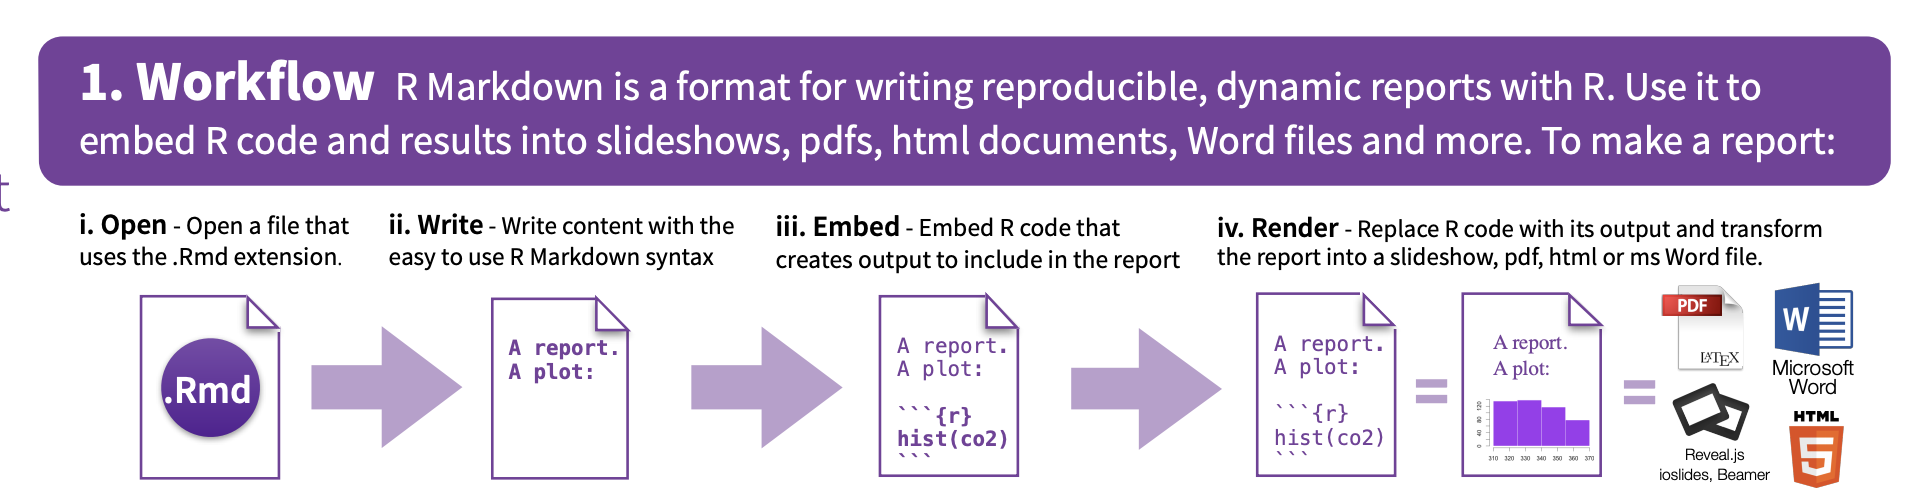
\includegraphics{images/workflow.png}
\caption{}
\end{figure}

\section{Opening a New File}\label{opening-a-new-file}

Writing R Markdown files is easiest within R Studio. Navigate to File
\textgreater{} New File \textgreater{} R Markdown to create a new file.

\begin{figure}
\centering
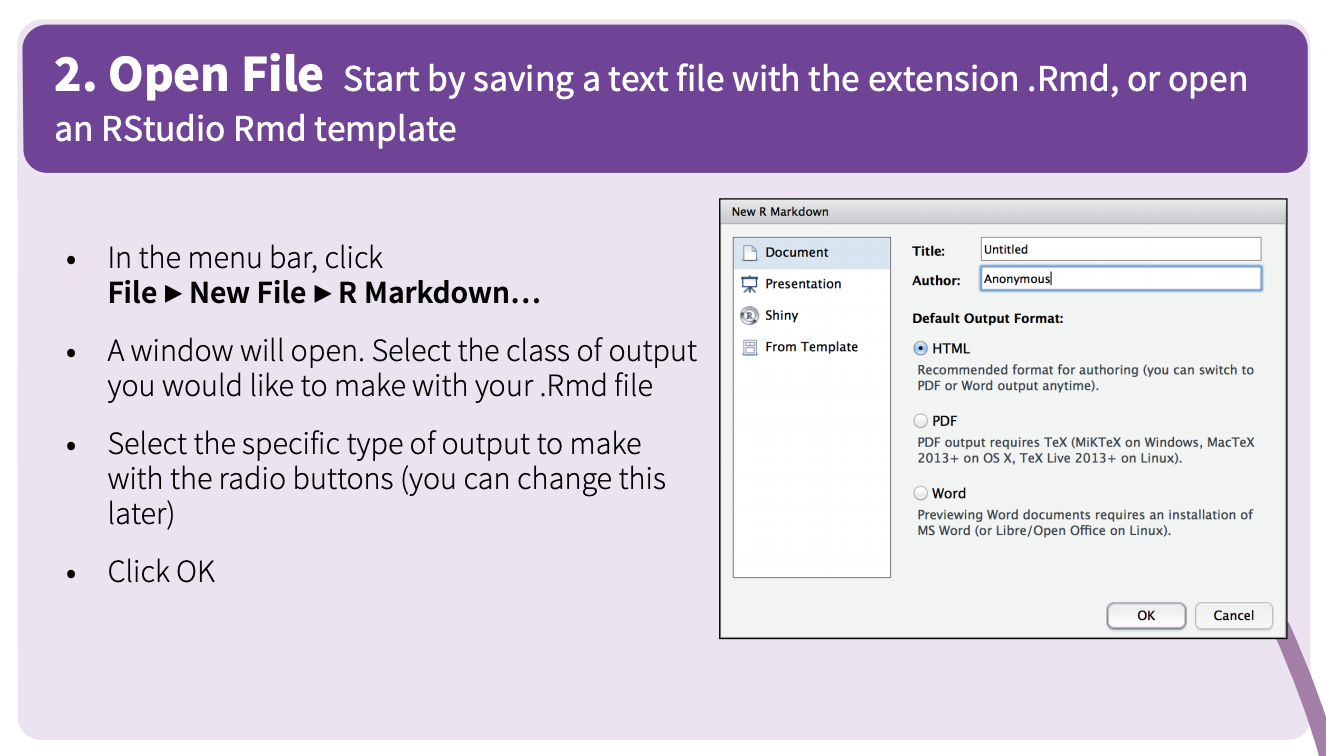
\includegraphics{images/open.png}
\caption{}
\end{figure}

\section{Helpful Syntax}\label{helpful-syntax}

Take a look through helpful sytax in this photo:

\begin{figure}
\centering
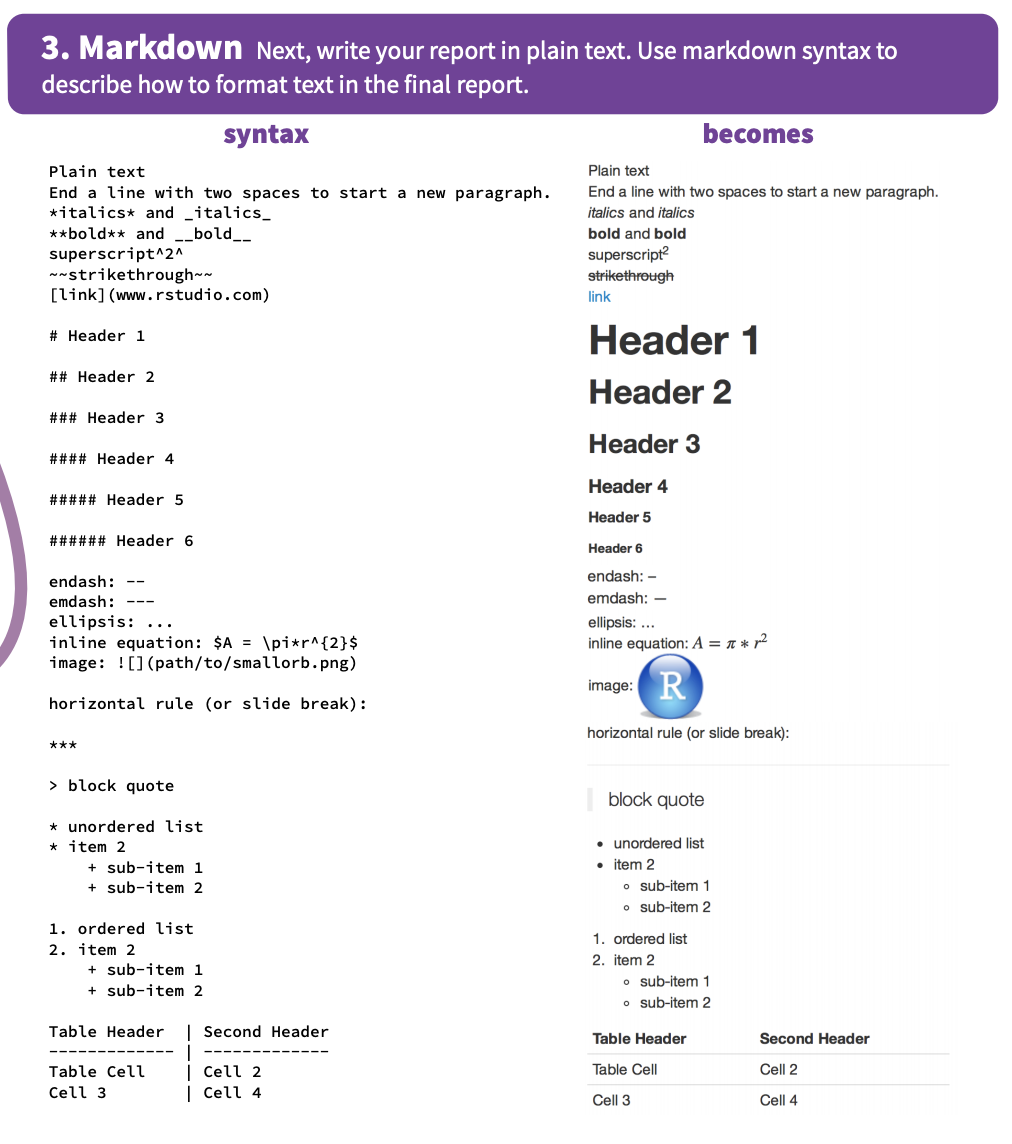
\includegraphics{images/syntax.png}
\caption{}
\end{figure}

Here are some examples to vie. Take a look at the raw R Markdown to view
the syntax in pratice.

\emph{italics} \textbf{bold} \sout{strikethrough}

\begin{quote}
Block Quote
\end{quote}

\begin{itemize}
\tightlist
\item
  Bullets
\item
  Bullets
\item
  subitem
\end{itemize}

\begin{enumerate}
\def\labelenumi{\arabic{enumi}.}
\tightlist
\item
  Lists
\item
  Lists
\end{enumerate}

\begin{itemize}
\tightlist
\item
  subitem
\end{itemize}

\section{Embed Code}\label{embed-code}

One of the best features of R Markdown is the ability to add code to
your document. To add a code snippet, click on the green \emph{insert}
button in your R Studio tool bar and choose which language you would
like to use!

\begin{Shaded}
\begin{Highlighting}[]
\KeywordTok{print}\NormalTok{(}\StringTok{"This is an R code snippet"}\NormalTok{)}
\end{Highlighting}
\end{Shaded}

\begin{verbatim}
## [1] "This is an R code snippet"
\end{verbatim}

\begin{Shaded}
\begin{Highlighting}[]
\BuiltInTok{print}\NormalTok{(}\StringTok{"This is a python code snippet with eval=FALSE"}\NormalTok{)}
\end{Highlighting}
\end{Shaded}

\begin{Shaded}
\begin{Highlighting}[]
\BuiltInTok{echo}\NormalTok{ this a bash code snippet}
\end{Highlighting}
\end{Shaded}

\begin{verbatim}
## this a bash code snippet
\end{verbatim}

\begin{figure}
\centering
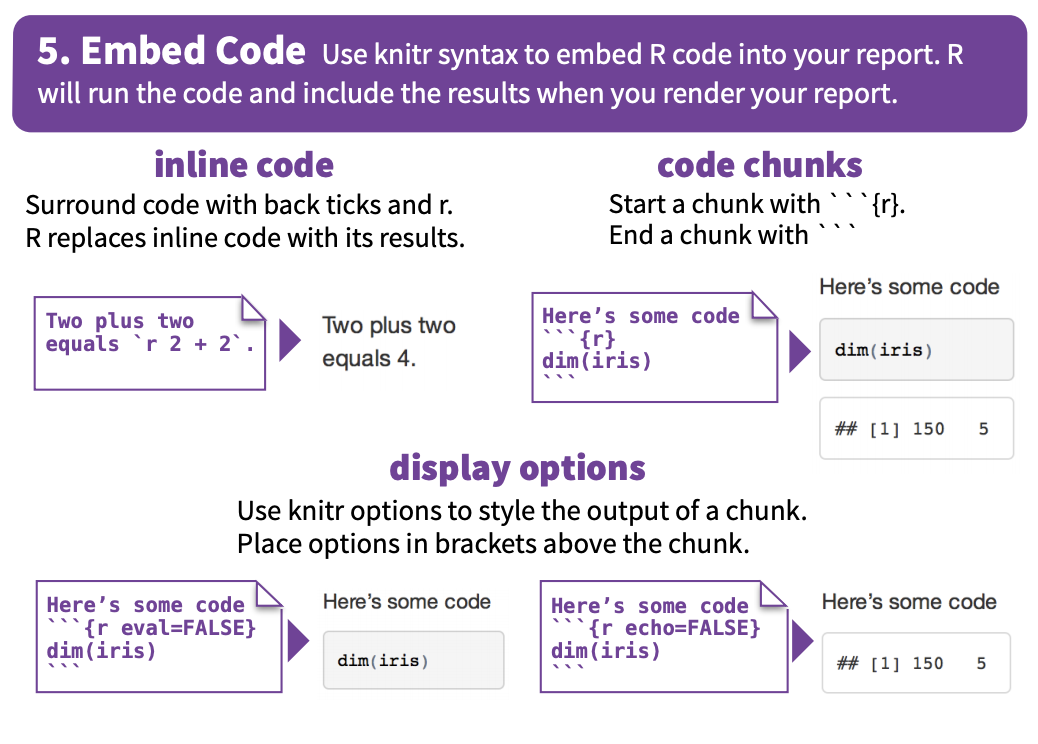
\includegraphics{images/code.png}
\caption{}
\end{figure}

There are also many options for your code snippets. Take a look:

\begin{figure}
\centering
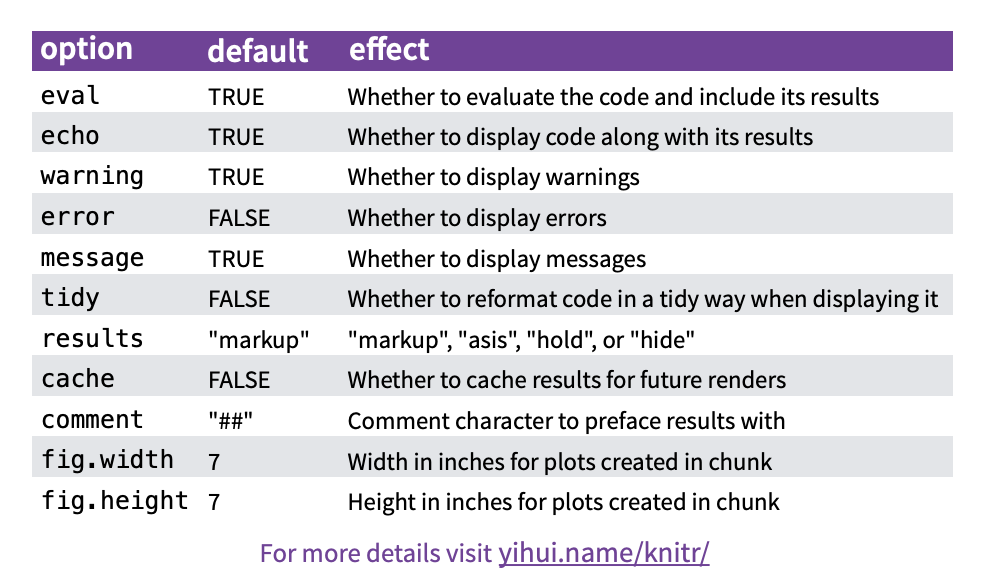
\includegraphics{images/options.png}
\caption{}
\end{figure}

\section{Wrapping (or knitting) it Up}\label{wrapping-or-knitting-it-up}

To knit your Markdown file you click the blue \emph{knit} button in your
R Studio toolbar. You can choose which file format you would like to
knit to as well!

For the purposes of our Merck-Data Mine documentation book, however, we
will not have to knit anything because we are placing the individual
documents in one bookdown book. To learn more about bookdown take a look
at \url{https://bookdown.org/yihui/bookdown/introduction.html} for more
information.

\chapter{Documentation Template}\label{documentation-template}

\section{Introduction}\label{introduction-1}

This section will give an overview of what was accomplished during the
previous sprint.

\section{Code}\label{code}

This section is where important code can be documented and commented on.
Some teams do not need to include all their code here as this would get
excessive. However, important functions or classes should be documented
and discussed here.

\section{Flow Diagrams /
Visualizations}\label{flow-diagrams-visualizations}

This is where teams should showcase flow diagrams of functions, data
pipeline, etc. This might also be a good place for
visualization/screenshots.

\section{White Paper}\label{white-paper}

When important decision are made, such as software specifications or
product developments, they should be documented in this section. Teams
should explain how they came to the conclusion and key takeaways about
the decision.

\section{Technical Report}\label{technical-report}

This section is where teams can highlight the processes of their work.
This is a more in depth look into what was accomplised during the sprint
where teams should describe step by step development.

\chapter{Data Engineering Fall 2020
Documentation}\label{data-engineering-fall-2020-documentation}

\section{Introduction to the Team}\label{introduction-to-the-team}

Our data engineering team is comprised of 6 team members all with unique
skills and backgrounds. The team worked hard to utilize each member's
strengths to help accomplish the semester goals for this project.

Include a brief sentence including your name, major, year, and relevant
experience to the data mine.

Jennifer Leising: I am a 3rd year graduate student in Industrial
Engineering. My research is focused on healthcare and data analytics,
and I have experience working in Clinical trials for a large Pharma
company.

Joshua Kosnoff: I am a junior majoring in biomedical engineering. I
perform research with the cancer research center, where I have
previously learned Python for data management and basic analysis.

Allison Hill: I am a senior majoring in electrical engineering. I have
coding experience in various languages, including some Python and R
which were used within this project.

Karthik Ravishankar: I am a freshman majoring in data science. I have
learned Java in highschool and at Purdue and some Python which was self
taught to contribute to the project.

Pranav Anandarao: I am a sophomore majoring in computer engineering. I
have experience in a few different programming languages, including
Python. I also have previous experience working on clinical
applications.

Eric Yap: I am sophomore majoring in data science and finance. Most of
my classes have helped developed my Python and R skills, which are very
transferable to the work I do in the data mine.

\section{Semester Goals}\label{semester-goals}

The overall aim of this project was to create a method to collect
continuous data from patients in clinical trials. The biometrics team
decided to do this by collecting data from Fitbit devices and developing
an application to collect supplementary data from the users.

The data engineering team's task was to collect the data and put it into
a usable format for storage with the data architecture team. This
semester, our goal was to add functionality to collect data from
multiple users and handle data coming in from different devices.
Furthermore, we would like to be able to schedule the program to collect
the user data periodically.

\section{Data Overview}\label{data-overview}

\subsection{Fitbit Devices vs.~Apple
Watch}\label{fitbit-devices-vs.apple-watch}

The 2019-2020 Merck Biometric team used the Fitbit to gather data for
the project. The Merck stakeholder's had also mentioend wanting to
explore the Apple Watch to reach additional populations. Our team wanted
to better understand what data was available from each company's
devices. As a note, we listed all the features that would be available
from any device. We created the chart below to list the features
available on each device. We found very similar data to be available on
both devices.

\begin{Shaded}
\begin{Highlighting}[]
\CommentTok{#                |                                       |Fitbit         |Apple Watch}
\CommentTok{# ---------------|---------------------------------------|---------------|---------------}
\CommentTok{# Activity       |Steps                                  |X              |X}
\CommentTok{#                |Workouts                               |X              |X}
\CommentTok{#                |Sit/Stand                              |X*             |NA}
\CommentTok{#                |Flight Climbed                         |X              |X}
\CommentTok{#                |Elevation                              |X              |X}
\CommentTok{#                |Time spent in different activity levels|X              |X}
\CommentTok{#                |Calories burned                        |X              |X}
\CommentTok{# Sleep          |Asleep vs Awake                        |X              |X}
\CommentTok{#                |Stages                                 |X              |NA}
\CommentTok{# Heart Rate     |Time spent in different heart ranges   |X              |3rd party apps}
\CommentTok{#                |Resting heart rate                     |X              |X}
\CommentTok{#                |Walking Heartrate                      |NA             |X}
\CommentTok{#                |Heart rate during activity             |X              |X}
\CommentTok{#                |Intraday Tracking                      |5 sec          |10 min}
\CommentTok{# Nutrition      |Food log*                              |X              |X}
\CommentTok{#                |Water log*                             |X              |X}
\CommentTok{# Body/Weight    |BMI*                                   |X              |X}
\CommentTok{#                |Weight*                                |X              |X}
\CommentTok{# Additional     |ECG                                    |Coming soon    |X}
\CommentTok{#                |Blood Oxygen                           |X              |X}
\CommentTok{#                |Fall Detection                         |X              |X}
\CommentTok{#                |Skin Thermometer                       |X              |NA}
\CommentTok{#                |Ear Health                             |NA             |X}
\CommentTok{#                |Stress Response                        |X              |NA}
\CommentTok{# ---------------------------------------------------------------------------------------}
\CommentTok{#    *Entered manually}
\CommentTok{#    NA = Not Available}
\end{Highlighting}
\end{Shaded}

With the Apple Watch, most data tracking is through the Health app and
the files are exported as a .xml, which is difficult to read. However,
you can also export your data through the Health app and have it opened
in Numbers/Excel for easy viewing. For the FitBit, activity is recorded
through the watch and outputs a .csv file when exporting, which is easy
to read and open in applications like Excel and Numbers.

Additionally, it appears we are able to use Python in order to
gather/sort data on both the Apple watch and Fitbit devices. Data is
able to be read through pandas. Since Apple Watch returns a .xml file,
we have to parse it first and use xmltodict module within Python before
we can start applying functions to our data.

Based on the scope for this semester, we did not do further research
into the Apple Watch data collection, but this is one of our goal's for
the coming Spring semester.

\subsection{Data Collected from Fitbit
Devices}\label{data-collected-from-fitbit-devices}

Our team collected data that can be grouped into several major
categories:

\begin{verbatim}
Device: Device Name

Activites: totalDistance, veryActiveDistance, moderatleyActiveDistance, lightlyActiveDistance, veryActiveMinutes, fairlyActiveMinutes, 
lightlyActiveMinutes, sedentaryMinutes, floorsClimbed, daySteps, intraday data

Sleep: sleepEfficiency, minutesAsleep

Heart Rate: HRrange30to100, HRrange100to140, HRrange140to170, HRrange170to220, avgRestingHR, intraday data

Weight: weight, BMI
\end{verbatim}

\section{Scaling the Framework}\label{scaling-the-framework}

The framework for collecting biometric data from Fitbit's API was
previously established and can be found in the
\href{https://nicholasrosenorn.github.io/wearables-book/tutorial-data-capture-in-python.html\#authentication}{Merck
Wearables Book section 8}. However, this framework could only be used to
collect one user's data at a time, and needed to be manually monitored
to switch between browser and python windows. Further, the framework
assumed that the user's Fitbit device would be the Fitbit Ionic. In
order to make this project upscalable, the framework needed to be
modified to support multiple users in an automizable way and to account
for multiple device types.

\subsection{Multiple Users}\label{multiple-users}

\subsubsection{Supporting Multiple Users Via Accessing
Credentials}\label{supporting-multiple-users-via-accessing-credentials}

To support multiple users, a database of multiple user login credentials
needed to be created. There is an ongoing collaboration with the Front
End team to create a more secure storage system, but for now credentials
are stored in a csv file with the format ``username,password''. With the
usernames and passwords stored in this way, a login array can be created
that will be used to plug into the automated process.

\begin{Shaded}
\begin{Highlighting}[]
\CommentTok{# Initialize Emails and Passwords lists}
\NormalTok{Emails }\OperatorTok{=}\NormalTok{ []}
\NormalTok{Passwords }\OperatorTok{=}\NormalTok{ []}
\CommentTok{# Create Emails and Passwords lists from Fitbit_Credentials.csv}
\ControlFlowTok{with} \BuiltInTok{open}\NormalTok{(}\StringTok{"Fitbit_Credentials.csv"}\NormalTok{) }\ImportTok{as}\NormalTok{ File1:}
\NormalTok{    IDs }\OperatorTok{=}\NormalTok{ csv.DictReader(File1)}
    \ControlFlowTok{for}\NormalTok{ row }\KeywordTok{in}\NormalTok{ IDs:}
\NormalTok{        Emails.append(row[}\StringTok{'Username'}\NormalTok{])}
\NormalTok{        Passwords.append(row[}\StringTok{'Password'}\NormalTok{])}
\end{Highlighting}
\end{Shaded}

As previously mentioned, the previous framework was not set up for
running through multiple accounts. To solve this issue, it was
reformatted into iterative-friendly components. The first of which is
the PythonBot.py file, which both establishes the login arrays outlined
above and is responsible for coordinating the other file and function
calls to make this process run smoothly.

\begin{Shaded}
\begin{Highlighting}[]
\CommentTok{# import other codes}
\ImportTok{import}\NormalTok{ BiometricPrevious}
\ImportTok{import}\NormalTok{ gather_keys_oauth2 }\ImportTok{as}\NormalTok{ Oauth2}
\KeywordTok{class}\NormalTok{ FitbitBot:}
    \KeywordTok{def} \FunctionTok{__init__}\NormalTok{(}\VariableTok{self}\NormalTok{, EMAIL, PASSWORD, DATE):}
        \CommentTok{#Both the Client ID and Client Secret come from when Fitbit site after registering an app}
\NormalTok{        CLIENT_ID }\OperatorTok{=} \StringTok{'22BH28'} 
\NormalTok{        CLIENT_SECRET }\OperatorTok{=} \StringTok{'78a4838804c1ff0983591e69196b1c46'}
        
        \CommentTok{#Authorization Process}
\NormalTok{        server }\OperatorTok{=}\NormalTok{ Oauth2.OAuth2Server(CLIENT_ID, CLIENT_SECRET)}
\NormalTok{        server.browser_authorize(EMAIL, PASSWORD)}
\NormalTok{        ACCESS_TOKEN }\OperatorTok{=} \BuiltInTok{str}\NormalTok{(server.fitbit.client.session.token[}\StringTok{'access_token'}\NormalTok{])}
\NormalTok{        REFRESH_TOKEN }\OperatorTok{=} \BuiltInTok{str}\NormalTok{(server.fitbit.client.session.token[}\StringTok{'refresh_token'}\NormalTok{])}
\NormalTok{        auth2_client }\OperatorTok{=}\NormalTok{ fitbit.Fitbit(CLIENT_ID, CLIENT_SECRET, Oauth2}\OperatorTok{=}\VariableTok{True}\NormalTok{, access_token}\OperatorTok{=}\NormalTok{ACCESS_TOKEN,}
\NormalTok{        refresh_token}\OperatorTok{=}\NormalTok{REFRESH_TOKEN)}
\NormalTok{        BiometricPrev }\OperatorTok{=}\NormalTok{ BiometricPrevious.FitbitModel1(auth2_client)}
        
\NormalTok{        biometricDF }\OperatorTok{=}\NormalTok{ BiometricPrev.getBiometricData(DATE) }\CommentTok{#append to data frame}
\NormalTok{        biometricDF.to_csv(}\StringTok{'./user'} \OperatorTok{+} \BuiltInTok{str}\NormalTok{(i) }\OperatorTok{+} \StringTok{'_'} \OperatorTok{+}\NormalTok{ DATE }\OperatorTok{+} \StringTok{'.csv'}\NormalTok{)}
        \BuiltInTok{print}\NormalTok{(}\StringTok{"Python Script Executed"}\NormalTok{)}
\CommentTok{# Run data extraction}
\ControlFlowTok{for}\NormalTok{ i }\KeywordTok{in} \BuiltInTok{range}\NormalTok{(}\BuiltInTok{len}\NormalTok{(Emails)):}
    \ControlFlowTok{for}\NormalTok{ j }\KeywordTok{in} \BuiltInTok{range}\NormalTok{(}\DecValTok{1}\NormalTok{): }\CommentTok{# Call the previous 1 days worth of info <-- will be replaced with cronjob}
\NormalTok{        today }\OperatorTok{=} \BuiltInTok{str}\NormalTok{((datetime.datetime.now() }\OperatorTok{-}\NormalTok{ datetime.timedelta(j)).strftime(}\StringTok{"%Y-%m-}\SpecialCharTok{%d}\StringTok{"}\NormalTok{))}
\NormalTok{        FitbitBot(Emails[i], Passwords[i], today)}
\end{Highlighting}
\end{Shaded}

The \emph{BiometricPrevious} file contains the remainder of the previous
framework with data collection functions, but it was also altered to
allow for multiple devices. More information about his can be found in
the \textbf{Multiple Devices} section of this report. The line
\emph{biometric.to\_csv} will store the collected data in a csv format
with a title of *user\#\_DATE\emph{, where }user\#* corresponds to the
order at which the user's login credentials are stored in the
credentials csv database.

\subsubsection{Supporting Multiple Users Via Allowing for
Automation}\label{supporting-multiple-users-via-allowing-for-automation}

In order to create an automation bot to regularly call the data
collection code (see \textbf{Scheduling Our Data Collection} for more
information on this), the code had to be adjusted so that it did not
open browser windows, as the opening of browser windows was found to
stall the bot. In order to accomplish this, the Selenium module was
used. Official Selenium documentation can be found
\href{https://selenium-python.readthedocs.io}{here}.

Since Selenium was not already downloaded on the device, it needed to be
installed. To do this, the following was typed into a Terminal window:

\begin{Shaded}
\begin{Highlighting}[]
\NormalTok{pip install selenium}
\end{Highlighting}
\end{Shaded}

To use Selenium in a code, the libraries and packages will need to be
imported. Since \emph{gather\_keys\_oauth2.py} is the only code package
responsible for accessing websites, Selenium only needs to be imported
into that document. To do this, the following code was added to
\emph{gather\_keys\_oauth2.py}.

\begin{Shaded}
\begin{Highlighting}[]
\ImportTok{from}\NormalTok{ selenium }\ImportTok{import}\NormalTok{ webdriver}
\ImportTok{from}\NormalTok{ selenium.webdriver }\ImportTok{import}\NormalTok{ Firefox}
\ImportTok{from}\NormalTok{ selenium.webdriver.firefox.options }\ImportTok{import}\NormalTok{ Options}
\ImportTok{from}\NormalTok{ selenium.webdriver.common.by }\ImportTok{import}\NormalTok{ By}
\end{Highlighting}
\end{Shaded}

Strictly speaking, the only explicitly needed code would be \emph{import
Selenium}. However, by importing specific functions from the Selenium
library upfront, notation later on was simplified. This can be seen
below when firefox options were set. Instead of calling
\emph{Selenium.webdriver.firefox.options} every line, \emph{Options} was
able to be called instead.

The appropriate Selenium firefox browser driver was downloaded
\href{https://github.com/mozilla/geckodriver/releases}{here}.

\textbf{Note} it does not matter where the driver is installed, but its
installation path needs to be plugged into the gather\_keys\_oath2.py
code. For those following along with the guide, make a note of the
installation path.

The following block of code was written to set the Selenium webdriver
functions.

\begin{Shaded}
\begin{Highlighting}[]
\NormalTok{firefox_options }\OperatorTok{=}\NormalTok{ Options()}
\NormalTok{firefox_options.add_argument(}\StringTok{"window-size=1920,1080"}\NormalTok{)}
\NormalTok{firefox_options.add_argument(}\StringTok{"--headless"}\NormalTok{)}
\NormalTok{firefox_options.add_argument(}\StringTok{"start-maximized"}\NormalTok{)}
\NormalTok{firefox_options.add_argument(}\StringTok{"--disable-infobars"}\NormalTok{)}
\NormalTok{firefox_options.add_argument(}\StringTok{"--disable-extensions"}\NormalTok{)}
\NormalTok{firefox_options.add_argument(}\StringTok{"--no-sandbox"}\NormalTok{)}
\NormalTok{firefox_options.add_argument(}\StringTok{"--disable-dev-shm-usage"}\NormalTok{)}
\NormalTok{firefox_options.binary_location }\OperatorTok{=} \StringTok{'/class/datamine/apps/firefox/firefox'}
\end{Highlighting}
\end{Shaded}

Adjust the path in the final option,
\emph{firefox\_options.binary\_location}, accordingly. The other main
option of interest is
\emph{firefox\_options.add\_argument(``--headless'')}. This
\emph{headerless} option is what allows the code to access the Fitbit
website without actually opening a browser -- effectively, Python
becomes a browser simulator. This is the main reason Selenium was used.
The other options are for optimal performance, but not strictly
necessary.

The first time an account is added, manual permissions will need to be
granted to Fitbit's authorization website. To do this, comment out this
headerless option (place a ``\#'' before the line), run the
\emph{PythonBot.py} code, and check the permissions boxes for each new
account as it pops up. After doing this once, uncomment this headerless
line. The system will then be ready for full automation.

The official Selenium documentation also supports a Google Chrome
driver. If Chrome is preferred, it can be substituted in for FireFox
without issue. However, make sure to change all instances of
\emph{firefox} in the above codes to \emph{Chrome.}

With Selenium downloaded and imported, the last step was to call and use
Selenium. The following line in \emph{browser\_authorize} function in
\emph{gather\_keys\_oauth2.py} was responsible for opening the web
browser, so it was targeted for edits.

\begin{Shaded}
\begin{Highlighting}[]
\NormalTok{    threading.Timer(}\DecValTok{1}\NormalTok{, webbrowser.}\BuiltInTok{open}\NormalTok{, args}\OperatorTok{=}\NormalTok{(url,)).start()}
\end{Highlighting}
\end{Shaded}

As its name might suggest, the \emph{webbrowser.open} function causes a
web browser to open. The other passed arguments \emph{1} and
\emph{args=(url,)} are parameters that can be left unchanged. This line
was replaced with the following code:

\begin{Shaded}
\begin{Highlighting}[]
\NormalTok{    driver }\OperatorTok{=}\NormalTok{ webdriver.Firefox(executable_path }\OperatorTok{=} \StringTok{'/class/datamine/apps/geckodriver'}\NormalTok{, options}\OperatorTok{=}\NormalTok{firefox_options)}
\NormalTok{    driver.get(}\StringTok{"https://accounts.fitbit.com/login?targetUrl=https%3A}\SpecialCharTok{%2F%2F}\StringTok{www.fitbit.com}\SpecialCharTok{%2F}\StringTok{us}\SpecialCharTok{%2F}\StringTok{home"}\NormalTok{)}
\NormalTok{    sleep(}\DecValTok{5}\NormalTok{)}
\NormalTok{    driver.find_element(By.XPATH, }\StringTok{"//input[@type='email']"}\NormalTok{).send_keys(email)}
\NormalTok{    sleep(}\DecValTok{2}\NormalTok{)}
\NormalTok{    driver.find_element(By.XPATH, }\StringTok{"//input[@type='password']"}\NormalTok{).send_keys(password)}
\NormalTok{    sleep(}\DecValTok{2}\NormalTok{)}
\NormalTok{    driver.find_element(By.XPATH, }\StringTok{"/html/body/div[2]/div/div[2]/div/div/div[3]/form/div[4]/div/button"}\NormalTok{).click()}
\NormalTok{    sleep(}\DecValTok{10}\NormalTok{)}
    
\NormalTok{    threading.Timer(}\DecValTok{1}\NormalTok{, driver.get, args}\OperatorTok{=}\NormalTok{(url,)).start()}
\end{Highlighting}
\end{Shaded}

The first line of the following code initializes the Selenium webdriver.
Edit the \emph{executable\_path} as needed based on where the firefox
driver was installed. The next line, \emph{driver.get}, tells the
Selenium web browser what website to go to. The \emph{find\_elements}
commands are what allow for the automatization of plugging in usernames
and emails. The sleep functions are input time delays to help make sure
that the website has time to properly load before attempting to log in.
The final line should look familiar. It is the same as the original
line, except replacing the \emph{webbrowser.open}, which opens a normal
web browser, with \emph{driver.get}, which calls Selenium's browser
simulator. The rest of \emph{gather\_keys\_oauth2} can remain as is.

\subsubsection{Moving to Scholar}\label{moving-to-scholar}

When multiple user logins were pushed and data extractions were
performed in relatively quick succession on personal Wi-Fi, Fitbit's
cybersecurity software flagged and temporarily banned the IP address
from accessing their site. While these bans can be overturned by
contacting Fitbit's customer support page on Twitter, the ``unbanning''
is temporary. This leads to a cycle of getting banned and asking to be
unbanned, which is both inconvenient and detrimental to any long term
data collection plans. The hope with Scholar is that, as an educational
IP address, it can be whitelisted and the automated process can function
without getting users banned.

\paragraph{Using Scholar}\label{using-scholar}

To access Scholar, go to
*\url{https://scholar-fe03.rcac.purdue.edu:300/main/*} and login with
Purdue 2 Factor Credentials.

The codes used for this part of the project are written in Python.
Unfortunately, Scholar does not currently support Python IDEs (Spyder,
VS code, etc). This means that the code either needs to be called
through a Jupyter Notebook Kernel or through a terminal window. For now,
the code will be run via Terminal commands.

To open Terminal, click on \textbf{Terminal Emulator} in Scholar's
applications bar. Once Terminal is open, navigate to the \emph{/class}
directory and then to the appropriate folder. To do this, type the
following commands into Terminal:

\begin{Shaded}
\begin{Highlighting}[]
\NormalTok{cd ..}
\NormalTok{cd ..}
\NormalTok{cd }\OperatorTok{/}\KeywordTok{class}\OperatorTok{/}\NormalTok{datamine}\OperatorTok{/}\NormalTok{corporate}\OperatorTok{/}\NormalTok{merck}\OperatorTok{/}\NormalTok{DataEngineers}\OperatorTok{/}\NormalTok{Fitbit}
\end{Highlighting}
\end{Shaded}

Needed files and libraries have been installed on Scholar. Pathways
within the code have been adjusted to Scholar's directory. As a result,
there is only one more step that needs to be done before the code can be
run. This step is to direct the python3 program where to find installed
libraries. Type the following command into the Terminal:

\begin{Shaded}
\begin{Highlighting}[]
\NormalTok{source }\OperatorTok{/}\KeywordTok{class}\OperatorTok{/}\NormalTok{datamine}\OperatorTok{/}\NormalTok{apps}\OperatorTok{/}\NormalTok{python.sh}
\end{Highlighting}
\end{Shaded}

\textbf{Note} You will need to rerun this command everytime you close
out of Terminal and reopen it.

Now, Scholar is ready to run PythonBot.py! To run the code, type the
following into Terminal:

\begin{Shaded}
\begin{Highlighting}[]
\NormalTok{python3 PythonBot.py}
\end{Highlighting}
\end{Shaded}

\textbf{Note} if the previous Terminal window was closed, navigate to
\emph{/class/datamine/corporate/merck/DataEngineers/Fitbit} again before
running \emph{python3 PythonBot.py}

Extracted data is formatted into CSV files and accessible at
\emph{/class/datamine/corporate/merck/DataEngineers/Fitbit/CSV\_Files}.

\subsection{Multiple Devices}\label{multiple-devices}

Not all fitbit devices have the same data available to them. This is
most noticeable in older models, in which functionality such as the
number of floors climbed or sleep cycles was not yet implemented. Using
the get\_Devices function available in the Fitbit API, the code returns
a string corresponding to the Fitbit version. For example, a Fitbit
Ionic would return the string ``Ionic''. Using this information, if-else
statements were implemented to check the version and assign
corresponding data values. Data that is not available would be input as
``None'' within the data table. In some cases, the function can simply
check if the data is NULL and automatically do this such as with the
sleep data. However for data such as activity levels, the data gets
input as a ``0'' instead and thus needs a check. Checks for some of the
newer models have been implemented, along with a generic case. The table
below shows the implemented models and their available data:

\begin{Shaded}
\begin{Highlighting}[]
 \CommentTok{#                |                                       |Ionic         | Versa Lite  |Inspire      |Charge 3     |}
 \CommentTok{# ---------------|---------------------------------------|--------------|-------------|-------------|-------------|}
 \CommentTok{# Activity       |Steps                                  |X             |X            |X            |X            |}
 \CommentTok{#                |Workouts                               |X             |X            |             |             |}
 \CommentTok{#                |Sit/Stand                              |X             |X            |             |             |}
 \CommentTok{#                |Flight Climbed                         |X             |             |             |             |}
 \CommentTok{#                |Elevation                              |X             |             |             |             |}
 \CommentTok{#                |Time spent in different activity levels|X             |X            |             |             |}
 \CommentTok{#                |Calories burned                        |X             |X            |             |             |}
 \CommentTok{# Sleep          |Asleep vs Awake                        |X             |X            |X            |X            |}
 \CommentTok{#                |Stages                                 |X             |X            |             |             |}
 \CommentTok{# Heart Rate     |Time spent in different heart ranges   |X             |X            |             |X            |}
 \CommentTok{#                |Resting heart rate                     |X             |X            |             |X            |}
 \CommentTok{#                |Walking Heartrate                      |X             |X            |             |X            |}
 \CommentTok{#                |Heart rate during activity             |X             |X            |             |X            |}
 \CommentTok{# -----------------------------------------------------------------------------------------------------------------}
\end{Highlighting}
\end{Shaded}

The following function is what is used to obtain the device model
string:

\begin{Shaded}
\begin{Highlighting}[]
\KeywordTok{def}\NormalTok{ getDevice():}
\NormalTok{    devices }\OperatorTok{=}\NormalTok{ auth2_client.get_devices()}
    \ControlFlowTok{if}\NormalTok{(}\BuiltInTok{len}\NormalTok{(devices) }\OperatorTok{==} \DecValTok{0}\NormalTok{):}
\NormalTok{        deviceVersion }\OperatorTok{=} \StringTok{'None'}
    \ControlFlowTok{else}\NormalTok{:}
\NormalTok{        deviceVersion }\OperatorTok{=}\NormalTok{ devices[}\DecValTok{0}\NormalTok{][}\StringTok{'deviceVersion'}\NormalTok{]    }
    \ControlFlowTok{return}\NormalTok{ deviceVersion}
\end{Highlighting}
\end{Shaded}

The function first calls the built-in Fitbit API get\_devices(). Next it
checks the length of the output to determine if it is valid. If it is
not valid, the user must not have any device registered. At the moment,
the code only obtains the first device if a user has multiple
registered.

\section{Scheduling the Data
Collection}\label{scheduling-the-data-collection}

Through using the CronTab module within Python, we are able to schedule
and run our FitBit functions on a routinely basis. The data we collect
is stored in a dataframe and new data is continuously appended to this
dataframe. The scheduled time is set to every 9 AM on weekdays.

\section{Collaborating with other
Teams}\label{collaborating-with-other-teams}

Our team had three main interactions with the other teams. The first one
was with the Data Architects. When reviewing last year's code, we
noticed that sending a CSV file everytime would be inneficient. We
discovered a function, dataFrame.to\_sql(), which would allow the data
to be sent straight into the SQL server. Although a solution was found,
we decided to leave the code how it is and save this idea for another
day. The second and third interactions were with the Front End team. The
first time, we wanted to see if there was a way to easily collect the
user's fitbit username and password. The Front End team was able to
create a way to have the login information collected from mobile app and
saved on the SQL server with the help of the Back End team. This was a
very important problem to solve as the API needs to log into the user's
fitbit account to pull their data. Our last collaboration was regarding
a issue that would result in complications during the clinical trial.
Regardless of whether the user is wearing their device or not, any time
the fitbit wasn't in an active motion, time is accrued on the user's
sedentary minutes. This would be a problem as there is no way to
differentiate whether the user was sedentary, or if the fitbit wasn't on
the user. After conversing with the Front End team, we decided that an
alert system or question during their survey would help solve this
issue. This problem is a work in progress and doesn't have a solution as
of yet.

\section{Future Work}\label{future-work}

Our future work for the Spring 2021 semester seeks to build upon our
work completed during this Fall 2020 semester. Our main goals are listed
include: (1) streamlining our work with the other Merck biometric teams
to ensure the entire process works well from start to finish, (2)
exploring alternative ways to access the user's fitbit information that
might better align with the way fitbit intends multiple user data
collection, and (3) investigating the collection of data from the Apple
Watch.

\begin{enumerate}
\def\labelenumi{(\arabic{enumi})}
\tightlist
\item
  Streamlining work with the other Merck Biometric teams
\item
  Exploring alternative ways to access the user's fitbit information
\item
  Investigating the collection of data from the Apple Watch
\end{enumerate}

\chapter{Data Engineering Spring 2021
Documentation}\label{data-engineering-spring-2021-documentation}

\section{Completing the Pipeline}\label{completing-the-pipeline}

In order to connect data collection process to the rest of the pipeline,
it had to be able to read patient information and login credentials from
the SQL database, as well as automatically append the collected
biometric data to a database. In order to accomplish this, the
PythonBot.py code had to be able to connect to SQL. This was done by
first importing the necessary sqlachemy pacakges and then establishing a
connection to our specific database.

To import packages:

\begin{Shaded}
\begin{Highlighting}[]
\CommentTok{# using sqlalchemy}
\ImportTok{import}\NormalTok{ sqlalchemy }\ImportTok{as}\NormalTok{ sal}
\ImportTok{from}\NormalTok{ sqlalchemy }\ImportTok{import}\NormalTok{ create_engine}
\ImportTok{import}\NormalTok{ pandas }\ImportTok{as}\NormalTok{ pd}
\end{Highlighting}
\end{Shaded}

To establish connection to SQL database:

\begin{Shaded}
\begin{Highlighting}[]
\CommentTok{# establish connecttion URL}
\NormalTok{conn }\OperatorTok{=} \StringTok{"mysql+pymysql://}\SpecialCharTok{\{0\}}\StringTok{:}\SpecialCharTok{\{1\}}\StringTok{@}\SpecialCharTok{\{2\}}\StringTok{:}\SpecialCharTok{\{3\}}\StringTok{/}\SpecialCharTok{\{4\}}\StringTok{"}\NormalTok{.}\BuiltInTok{format}\NormalTok{(}
    \StringTok{'cb3i17t0aqn6a4ff'}\NormalTok{, }\StringTok{'e2l4k9zn24shcj42'}\NormalTok{, }\StringTok{'rnr56s6e2uk326pj.cbetxkdyhwsb.us-east-1.rds.amazonaws.com'}\NormalTok{, }\StringTok{'3306'}\NormalTok{, }\StringTok{'lfry112yqr3k2dfr'}\NormalTok{)}
 
\CommentTok{# create engine}
\NormalTok{engine }\OperatorTok{=}\NormalTok{ sal.create_engine(conn)}
\end{Highlighting}
\end{Shaded}

If another SQL database is used in the future, please note that
`cb3i17t0aqn6a4ff' corresponds to `username', `e2l4k9zn24shcj42'
corresponds to `password',
`rnr56s6e2uk326pj.cbetxkdyhwsb.us-east-1.rds.amazonaws.com' corresponds
to `address', `3306' corresponds to `port', and `lfry112yqr3k2dfr'
corresponds to `DB'. Change these values as appropriate in the code.

\subsection{Reading in user data from patient
table}\label{reading-in-user-data-from-patient-table}

Patient data was imported as a series of arrays. The SQL patient table
was read in as df1, which was used to form lists of data corresponding
to individual patient's emails, passwords, IDs, and usernames.

\begin{Shaded}
\begin{Highlighting}[]
\NormalTok{df1 }\OperatorTok{=}\NormalTok{ pd.read_sql_query(}\StringTok{"SELECT * FROM patient"}\NormalTok{, engine)}
\NormalTok{emails }\OperatorTok{=}\NormalTok{ []}
\NormalTok{passwords }\OperatorTok{=}\NormalTok{ []}
\NormalTok{IDs }\OperatorTok{=}\NormalTok{ []}
\NormalTok{usernames }\OperatorTok{=}\NormalTok{ []}
\ControlFlowTok{for}\NormalTok{ i }\KeywordTok{in} \BuiltInTok{range}\NormalTok{(}\BuiltInTok{len}\NormalTok{(df1)):}
\NormalTok{    emails.append(df1.email[i])}
\NormalTok{    passwords.append(df1.fitbit_password[i])}
\NormalTok{    IDs.append(df1.patient_id[i])}
\NormalTok{    usernames.append(df1.username[i])}
\end{Highlighting}
\end{Shaded}

As was previously the case, this data was iterated through and plugged
into the FitbitBot function.

\subsection{Appending user data to SQL
table}\label{appending-user-data-to-sql-table}

Once data was collected (collection functions can be found in
\emph{BiometricPrevious\_getDevice\_v2.py}), it needed to be appended to
the SQL database. A new function was made to reformat the data to have
the same column names as the SQL table.

\begin{Shaded}
\begin{Highlighting}[]
\KeywordTok{def}\NormalTok{ appendDataBase(DATA,ENGINE, USER, ID):}
\NormalTok{    obj }\OperatorTok{=}\NormalTok{ pd.DataFrame()}
   
\NormalTok{    obj[}\StringTok{'patient_id'}\NormalTok{] }\OperatorTok{=}\NormalTok{ [ID]}
\NormalTok{    obj[}\StringTok{'fbusername'}\NormalTok{] }\OperatorTok{=}\NormalTok{ [USER]}
\NormalTok{    obj[}\StringTok{'collection_date'}\NormalTok{] }\OperatorTok{=}\NormalTok{ [DATA.get(}\StringTok{"Date"}\NormalTok{)]}
\NormalTok{    obj[}\StringTok{'steps'}\NormalTok{] }\OperatorTok{=}\NormalTok{ [DATA.get(}\StringTok{"Steps"}\NormalTok{)]}
\NormalTok{    obj[}\StringTok{'floors_climbed'}\NormalTok{] }\OperatorTok{=}\NormalTok{ [DATA.get(}\StringTok{"Floors Climbed"}\NormalTok{)]}
\NormalTok{    obj[}\StringTok{'total_miles'}\NormalTok{] }\OperatorTok{=}\NormalTok{ [DATA.get(}\StringTok{"Total Miles"}\NormalTok{)]}
\NormalTok{    obj[}\StringTok{'lightly_active_miles'}\NormalTok{] }\OperatorTok{=}\NormalTok{ [DATA.get(}\StringTok{"Lightly Active Miles"}\NormalTok{)]}
\NormalTok{    obj[}\StringTok{'moderately_active_miles'}\NormalTok{] }\OperatorTok{=}\NormalTok{ [DATA.get(}\StringTok{"Moderately Active Miles"}\NormalTok{)]}
\NormalTok{    obj[}\StringTok{'very_active_miles'}\NormalTok{] }\OperatorTok{=}\NormalTok{ [DATA.get(}\StringTok{"Very Active Miles"}\NormalTok{)]}
\NormalTok{    obj[}\StringTok{'sedentary_minutes'}\NormalTok{] }\OperatorTok{=}\NormalTok{ [DATA.get(}\StringTok{"Sedentary Minutes"}\NormalTok{)]}
\NormalTok{    obj[}\StringTok{'lightly_active_minutes'}\NormalTok{] }\OperatorTok{=}\NormalTok{ [DATA.get(}\StringTok{"Lightly Active Minutes"}\NormalTok{)]}
\NormalTok{    obj[}\StringTok{'fairly_active_minutes'}\NormalTok{] }\OperatorTok{=}\NormalTok{ [DATA.get(}\StringTok{"Fairly Active Minutes"}\NormalTok{)]}
\NormalTok{    obj[}\StringTok{'very_active_minutes'}\NormalTok{] }\OperatorTok{=}\NormalTok{ [DATA.get(}\StringTok{"Very Active Minutes"}\NormalTok{)]}
\NormalTok{    obj[}\StringTok{'hr30_100_minutes'}\NormalTok{] }\OperatorTok{=}\NormalTok{ [DATA.get(}\StringTok{"HR 30-100 Minutes"}\NormalTok{)]}
\NormalTok{    obj[}\StringTok{'hr100_140_minutes'}\NormalTok{] }\OperatorTok{=}\NormalTok{ [DATA.get(}\StringTok{"HR 100-140 Minutes"}\NormalTok{)]}
\NormalTok{    obj[}\StringTok{'hr140_170_minutes'}\NormalTok{] }\OperatorTok{=}\NormalTok{ [DATA.get(}\StringTok{"HR 140-170 Minutes"}\NormalTok{)]}
\NormalTok{    obj[}\StringTok{'hr170_220_minutes'}\NormalTok{] }\OperatorTok{=}\NormalTok{ [DATA.get(}\StringTok{"HR 170-220 Minutes"}\NormalTok{)]}
\NormalTok{    obj[}\StringTok{'average_resting_hr'}\NormalTok{] }\OperatorTok{=}\NormalTok{ [DATA.get(}\StringTok{"Average Resting HR"}\NormalTok{)]}
\NormalTok{    obj[}\StringTok{'bmi'}\NormalTok{] }\OperatorTok{=}\NormalTok{ DATA.get(}\StringTok{"BMI"}\NormalTok{)}
\NormalTok{    obj[}\StringTok{'sleep_efficiency'}\NormalTok{] }\OperatorTok{=}\NormalTok{ DATA.get(}\StringTok{"Sleep Efficiency"}\NormalTok{)}
\NormalTok{    obj[}\StringTok{'weight'}\NormalTok{] }\OperatorTok{=}\NormalTok{ DATA.get(}\StringTok{"Weight"}\NormalTok{)}
\NormalTok{    obj[}\StringTok{"minutes_asleep"}\NormalTok{] }\OperatorTok{=}\NormalTok{ todaysData.get(}\StringTok{"Minutes Alseep"}\NormalTok{)}
 
\NormalTok{    obj.to_sql(}\StringTok{"fitbit_data"}\NormalTok{, con}\OperatorTok{=}\NormalTok{ENGINE, if_exists}\OperatorTok{=}\StringTok{'append'}\NormalTok{, index}\OperatorTok{=} \VariableTok{False}\NormalTok{)}
   
    \ControlFlowTok{return}\NormalTok{(}\VariableTok{None}\NormalTok{)}
\end{Highlighting}
\end{Shaded}

In this function, the argument \emph{DATA} is a dataframe returned from
\emph{biometric\_previous\_getDevice\_v2.py}, \emph{ENGINE} is the
connection engine to the SQL database, and \emph{USER} and \emph{ID}
correspond to the user's Fitbit username and Merck trial userID. The
\emph{to\_sql} function at the end is responsible for exporting the
reformatted data to the \emph{``fitbit\_data''} table in the SQL
database. The \emph{if\_exists=`append'} argument is responsible for
appending to the database instead of overwriting it, and the
\emph{index=False} argument stops the code from creating the original
indexing as a column in SQL.

More documentation on .to\_sql can be found here:
\url{https://pandas.pydata.org/docs/reference/api/pandas.DataFrame.to_sql.html}

In order to pass the userID and fitbit username to the SQL database, the
FitbitBot function and function call had to be slightly altered.

\begin{Shaded}
\begin{Highlighting}[]
\KeywordTok{class}\NormalTok{ FitbitBot:}
    \KeywordTok{def} \FunctionTok{__init__}\NormalTok{(}\VariableTok{self}\NormalTok{, EMAIL, PASSWORD, DATE, usernames, ID):}
 
        \CommentTok{#Both the Client ID and Client Secret come from when Fitbit site after registering an app}
\NormalTok{        CLIENT_ID }\OperatorTok{=} \StringTok{'22BH28'} \CommentTok{#Mine:'22BKP3'}
\NormalTok{        CLIENT_SECRET }\OperatorTok{=} \StringTok{'78a4838804c1ff0983591e69196b1c46'} \CommentTok{#Mine:'1a42e97b6b4cc640572ae5cf10a7d0b0'}
        \CommentTok{#Authorization Process}
        \CommentTok{# opens website}
\NormalTok{        server }\OperatorTok{=}\NormalTok{ Oauth2.OAuth2Server(CLIENT_ID, CLIENT_SECRET)}
        \CommentTok{# opens website}
\NormalTok{        server.browser_authorize(EMAIL, PASSWORD)}
\NormalTok{        ACCESS_TOKEN }\OperatorTok{=} \BuiltInTok{str}\NormalTok{(server.fitbit.client.session.token[}\StringTok{'access_token'}\NormalTok{])}
\NormalTok{        REFRESH_TOKEN }\OperatorTok{=} \BuiltInTok{str}\NormalTok{(server.fitbit.client.session.token[}\StringTok{'refresh_token'}\NormalTok{])}
\NormalTok{        auth2_client }\OperatorTok{=}\NormalTok{ fitbit.Fitbit(CLIENT_ID, CLIENT_SECRET, Oauth2}\OperatorTok{=}\VariableTok{True}\NormalTok{, access_token}\OperatorTok{=}\NormalTok{ACCESS_TOKEN,}
\NormalTok{        refresh_token}\OperatorTok{=}\NormalTok{REFRESH_TOKEN)}
\NormalTok{        BiometricPrev }\OperatorTok{=}\NormalTok{ BiometricPrevious.FitbitModel1(auth2_client)}
\NormalTok{        bioDict, biometricDF }\OperatorTok{=}\NormalTok{ BiometricPrev.getBiometricData(DATE) }\CommentTok{#append to data frame}
\NormalTok{        title }\OperatorTok{=} \StringTok{'./CSV_Files/user'} \OperatorTok{+} \BuiltInTok{str}\NormalTok{(i) }\OperatorTok{+} \StringTok{'_'} \OperatorTok{+}\NormalTok{ DATE }\OperatorTok{+} \StringTok{'.csv'}
\NormalTok{        appendDataBase(bioDict,engine,usernames,ID)}
        \BuiltInTok{print}\NormalTok{(}\StringTok{"Python Script Executed"}\NormalTok{)}
\end{Highlighting}
\end{Shaded}

usernames and ID arguments were added to the function. The
appendDataBase function call was also added into the function, and
BiometricPrev.getBiometricData(DATA) was slightly altered to return both
a dictionary and a database.

Since the function arguments were exanded, the function call also had to
be adjusted to pass usernames{[}i{]} and IDs{[}i{]}.

\begin{Shaded}
\begin{Highlighting}[]
\NormalTok{today }\OperatorTok{=} \BuiltInTok{str}\NormalTok{((datetime.datetime.now() }\OperatorTok{-}\NormalTok{ datetime.timedelta(}\DecValTok{1}\NormalTok{)).strftime(}\StringTok{"%Y-%m-}\SpecialCharTok{%d}\StringTok{"}\NormalTok{))}
\CommentTok{# Run data extraction}
\ControlFlowTok{for}\NormalTok{ i }\KeywordTok{in} \BuiltInTok{range}\NormalTok{(}\BuiltInTok{len}\NormalTok{(emails)):}
\NormalTok{    FitbitBot(emails[i], passwords[i], today, usernames[i], IDs[i])}
\end{Highlighting}
\end{Shaded}

\section{Automating the Pipeline}\label{automating-the-pipeline}

Automating the process was done two different ways. One was done through
Cronjob and is useful for UNIX (Mac, linux) operating systems. This was
used while the code was on Scholar. However, Scholar had period cronjob
wipes, which meant that the automated process had to continually be
re-established (and that defeated the purpose!). As a result, the code
stopped being run on Scholar and was moved onto the Merck E2C AWS
server. This was Windows based, so Task Scheduler was used.

\subsection{Cronjob (for Mac and
Linux)}\label{cronjob-for-mac-and-linux}

Open Terminal. To see a list of current cronjob, type the following:

\begin{Shaded}
\begin{Highlighting}[]
\NormalTok{crontab }\OperatorTok{-}\NormalTok{l}
\end{Highlighting}
\end{Shaded}

To edit a crontab or edit an existing one:

\begin{Shaded}
\begin{Highlighting}[]
\NormalTok{crontab }\OperatorTok{-}\NormalTok{e}
\end{Highlighting}
\end{Shaded}

Type \emph{i} to enter INSERT mode. Enter your cronjob command. For the
case of this project on scholar, the following was used:

\begin{Shaded}
\begin{Highlighting}[]
\DecValTok{0} \DecValTok{1} \OperatorTok{*} \OperatorTok{*} \OperatorTok{*}\NormalTok{ cd }\OperatorTok{/}\KeywordTok{class}\OperatorTok{/}\NormalTok{datamine}\OperatorTok{/}\NormalTok{corporate}\OperatorTok{/}\NormalTok{merck}\OperatorTok{/}\NormalTok{DataEngineers}\OperatorTok{/}\NormalTok{Fitbit }\OperatorTok{&&} \OperatorTok{/}\KeywordTok{class}\OperatorTok{/}\NormalTok{datamine}\OperatorTok{/}\NormalTok{apps}\OperatorTok{/}\NormalTok{python}\OperatorTok{/}\NormalTok{f2020}\OperatorTok{-}\NormalTok{s2021}\OperatorTok{/}\NormalTok{env}\OperatorTok{/}\BuiltInTok{bin}\OperatorTok{/}\NormalTok{python3}\FloatTok{.8}\NormalTok{ PythonBot.py}
\end{Highlighting}
\end{Shaded}

The first 5 characters are timing instructions. The first one (0)
corresponds to the minute. The second (1) corresponds to the hour. The
3rd corresponds to the day of the month, then month, then day of the
week. An asterisk indicates that the job will run for every value in
those corresponding categories. As a result

\begin{Shaded}
\begin{Highlighting}[]
\DecValTok{0} \DecValTok{1} \OperatorTok{*} \OperatorTok{*} \OperatorTok{*} 
\end{Highlighting}
\end{Shaded}

will run everyday at 1am.

\emph{cd} navigates to a file directory. \textbf{Note} that if your
python functions are in PATH, you can navigate to your file directly
before issuing the crontab -e command, in which case you can simply
type:

\begin{Shaded}
\begin{Highlighting}[]
\DecValTok{0} \DecValTok{1} \OperatorTok{*} \OperatorTok{*} \OperatorTok{*}\NormalTok{ PythonBot.py}
\end{Highlighting}
\end{Shaded}

However, since python is not currently in PATH on scholar, the path to
both the desired code (PythonBot.py) and had to be indicated in the
command.

Type \emph{:wq} to write the command and quit Insert mode. Type crontab
-l in Terminal to confirm set up.

\subsection{Task Scheduler (Windows)}\label{task-scheduler-windows}

Windows provides a GUI for their scheduling program. To open it, click
on the microscope search icon in the bottom of the screen (or right
click on the windows icon and select `search') and type \emph{Task
Scheduler}. Open the application.

In the \emph{Actions} sidebar, click on \emph{Create Task}. Name the
program and navigate to the \emph{Triggers} tab. The trigger tab is
tells Windows how often to run the program. Add a new trigger by
clicking on \emph{New}. Specify how often to run the program. The
current project was made to run everyday at 1 am, and this was
accomplished by selecting \emph{Daily}, adjusting the start time to 1am,
and clicking \emph{ok}.

\textbf{Note} The E2C instance is not based in EST time. Make sure that
your entered time is actually your desired time.

Now its time to tell the Task Scheduler what program to actually run.
Click on the \emph{Actions} tab and add a new action. Browse for the
script to automate. Click \emph{ok}. The \emph{Conditions} and
\emph{Settings} tabs offer more customization, but are not needed for
the purposes of this project. Click \emph{ok} to save the task.

The added ask should show up in the main page of the GUI. Confirm that
it does and that its status is \emph{Enabled}. If its status is
\emph{Disabled}, right click on the task and select \emph{Enable}.

The program is now ready to run automatically!

\section{Exploring Apple HealthKit and
XCode}\label{exploring-apple-healthkit-and-xcode}

Our team decided to start looking into creating the data aquisition
script for the Apple Watch. This led us to Apple HealthKit. HealthKit
allows access to and the ability to share health and fitness data that
is collected using an iPhone and/or Apple Watch. We explored the the
documentation that Apple had to offer and began learning how to use
HealthKit. To use HealthKit to access the user's health data, we had to
begin learning the language Swift and the IDE, XCode The problem we
quickly encountered was that this could only be fully explored on Apple
devices. In addition to exploring HealthKit and XCode on our own, we
also searched for resources that we could use to assist in developing
the data aquisition script. A lot of what we found was able to read and
write the data but not export the data. Our current plan is to utilize a
code template that walks through the authentication and data collection
process and then directly send the data to the AWS database.

A few other options exist for collecting the data from the Apple Watch.
React Native can be used to develop an IOS application to collect and
store the data fron the watch. However, apple devices are still needed
to build and deploy the application, and thus not providing much
advantage over a Swift based application. Another method to collect the
data could be to utilize Google Fit and the pre-existing Google API.
This would require the user to download the Google Fit application on
their phone and signing in, which creates an intermediary that wouldn't
be necessary in the other implementations. In the end, these two other
implementations were not used in favor of the Swift implementation.

\section{Thank you \&
Acknowledgements}\label{thank-you-acknowledgements}

We would like to thank our Merck Corporate Partners, TA, and all the
Data Mine staff that have helped us throughout this semester.

\chapter{Data Architects}\label{data-architects}

\section{What is a database?}\label{what-is-a-database}

A database is an organized collection of data stored electronically. It
is typically controlled by a database management system (DBMS). There
are two main categories a database can fall into: relational and
non-relational. A relational database is one that stores data in rows
and columns, otherwise known as a table. While a simple database may
include only one table, a typical functional database contains multiple
tables. These tables are linked to each other using keys. A primary key
is a unique identifier and is referenced by other tables. When in
another table, it is considered a foreign key. While it is not
necessary, it is common practice to include a primary key in every
table. Nearly all relational databases rely on the programming language
SQL (Structured Query Language) to query, manipulate, and define data,
as well as provide access control.

The term ``non-relational database'' is a blanket term for all other
databases that do not rely on SQL, hence their other name, NoSQL. These
databases can take on many forms: key-value store, document store,
column-oriented databases, and graph databases, to name a few.

\section{How to create the database:}\label{how-to-create-the-database}

First step would be to download mySQL on a machine.
\url{https://www.mysql.com/} is the website where the software can be
downloaded. Click on ``Downloads'' on the top of the tabs, and scroll
down to click on MySQL Community (GPL) Downloads. Next click on ``MySQL
Community Downloads''. Please select the correct operating system based
on your machine type. Also, make sure to check system versions and
download archives based on the critias. After downloading this go back
and click on MySQL Workbench downloads. Make sure to follow the previous
instructions and download the workbench similar to how communities were
downloaded.

Once everything is downloaded please go into mySQL. Make sure to set a
good password for your connection. Once in MySQL click on Local
instance. The script for the database including the comments it written
below. In order to transfer the database into your own system please
paste the script into your mySQL. After pasting everything in click on
the lighting shape button with a one symbol to run your code.

\section{Basic SQL key:}\label{basic-sql-key}

-- (Whenever there is a comment amongst the code this is typed before
the comment. Similar to \# in python)

VARCHAR(): this is character data. The number in the parenthesis is the
amount of characters in the word saved in the tables.

FLOAT: this stores an approximate value and decimal. An example would be
that monet data would use FLOAT.

INT: This is a data type that is a primary integer data type.

\section{MySQL Script:}\label{mysql-script}

-- This is the code that loads different settings into your database. --
MySQL Workbench Forward Engineering

/\emph{!40101 SET
\citet{OLD_CHARACTER_SET_CLIENT}=@\citet{CHARACTER_SET_CLIENT} }/;
/\emph{!40101 SET
\citet{OLD_CHARACTER_SET_RESULTS}=@\citet{CHARACTER_SET_RESULTS} }/;
/\emph{!40101 SET
\citet{OLD_COLLATION_CONNECTION}=@\citet{COLLATION_CONNECTION} }/;
/\emph{!40101 SET NAMES utf8 }/; /\emph{!40103 SET
\citet{OLD_TIME_ZONE}=@\citet{TIME_ZONE} }/; /\emph{!40103 SET
TIME\_ZONE=`+00:00' }/; /\emph{!40014 SET
\citet{OLD_UNIQUE_CHECKS}=@\citet{UNIQUE_CHECKS}, UNIQUE\_CHECKS=0 }/;
/\emph{!40014 SET
\citet{OLD_FOREIGN_KEY_CHECKS}=@\citet{FOREIGN_KEY_CHECKS},
FOREIGN\_KEY\_CHECKS=0 }/; /\emph{!40101 SET
\citet{OLD_SQL_MODE}=@\citet{SQL_MODE},
SQL\_MODE=`NO\_AUTO\_VALUE\_ON\_ZERO' }/; /\emph{!40111 SET
\citet{OLD_SQL_NOTES}=@\citet{SQL_NOTES}, SQL\_NOTES=0 }/;

\begin{longtable}[]{@{}ll@{}}
\toprule
-- & This is the first table for the Merck database. CREATE TABLE IF NOT
EXISTS notifies mySQL to create a new table. After this would be the
name for the table.\tabularnewline
\midrule
\endhead
-- & Schema Merck database\tabularnewline
\bottomrule
\end{longtable}

CREATE SCHEMA IF NOT EXISTS \texttt{Merck\ database} DEFAULT CHARACTER
SET utf8 ; USE \texttt{Merck\ database} ; --
----------------------------------------------------- -- Table
\texttt{Merck\ database}.\texttt{User}: This table will store
information for the website. When the user first creates an account. --
----------------------------------------------------- CREATE TABLE IF
NOT EXISTS \texttt{Merck\ database}.\texttt{User} ( \texttt{id} INT NOT
NULL, \texttt{username} VARCHAR(20) NOT NULL, \texttt{First\_Name}
VARCHAR(100) NOT NULL, \texttt{Last\_Name} VARCHAR(100) NOT NULL,
\texttt{date\_of\_birth} INT NOT NULL, \texttt{Height} INT NOT NULL,
PRIMARY KEY (\texttt{id}), UNIQUE INDEX \texttt{username\_UNIQUE}
(\texttt{username} ASC)) ENGINE = InnoDB; --
----------------------------------------------------- -- Table
\texttt{Merck\ database}.\texttt{MerckData}: This is the table that will
store the written data in the website. --
------------------------------------------------------ CREATE TABLE IF
NOT EXISTS \texttt{Merck\ database}.\texttt{MerckData} ( \texttt{ID} INT
NOT NULL, \texttt{input\_date} INT NOT NULL,
\texttt{family\_history\_cancer} VARCHAR(500) NULL,
\texttt{Family\_history\_heart\_disease} VARCHAR(500) NULL,
\texttt{diagnostic\_notes} VARCHAR(500) NULL, PRIMARY KEY (\texttt{ID}))
ENGINE = InnoDB; --
----------------------------------------------------- -- Table
\texttt{Merck\ database}.\texttt{Pain\_Data}: This is the data that the
patient inputs themselves. --
----------------------------------------------------- CREATE TABLE IF
NOT EXISTS \texttt{Merck\ database}.\texttt{Pain\_Data} (
\texttt{Username} VARCHAR(20) NOT NULL, \texttt{input\_date} DATETIME
NOT NULL, \texttt{happiness} FLOAT NULL, \texttt{Sleep} FLOAT NULL,
\texttt{hours\_worked} FLOAT NULL, \texttt{Symptoms} VARCHAR(100) NULL,
\texttt{Meals} FLOAT NULL, \texttt{medication\_timing} VARCHAR(200)
NULL, \texttt{smoking\_alcohol} VARCHAR(200) NULL,
\texttt{Other\_medication} VARCHAR(200) NULL, \texttt{water\_intake}
FLOAT NULL, \texttt{diagnosis} VARCHAR(300) NULL, PRIMARY KEY
(\texttt{Username})) ENGINE = InnoDB; --
----------------------------------------------------- -- Table
\texttt{Merck\ database}.\texttt{User\_MerckData}: This is the script
that will connect the Merck database and User\_MerckData. --
----------------------------------------------------- CREATE TABLE IF
NOT EXISTS \texttt{Merck\ database}.\texttt{User\_MerckData} (
\texttt{User\_id} INT NOT NULL, \texttt{MerckData\_ID} INT NOT NULL,
PRIMARY KEY (\texttt{User\_id}, \texttt{MerckData\_ID}), INDEX
\texttt{fk\_User\_has\_MerckData\_MerckData1\_idx}
(\texttt{MerckData\_ID} ASC), INDEX
\texttt{fk\_User\_has\_MerckData\_User\_idx} (\texttt{User\_id} ASC),
CONSTRAINT \texttt{fk\_User\_has\_MerckData\_User} FOREIGN KEY
(\texttt{User\_id}) REFERENCES \texttt{Merck\ database}.\texttt{User}
(\texttt{id}) ON DELETE NO ACTION ON UPDATE NO ACTION, CONSTRAINT
\texttt{fk\_User\_has\_MerckData\_MerckData1} FOREIGN KEY
(\texttt{MerckData\_ID}) REFERENCES
\texttt{Merck\ database}.\texttt{MerckData} (\texttt{ID}) ON DELETE NO
ACTION ON UPDATE NO ACTION) ENGINE = InnoDB; --
----------------------------------------------------- -- Table
\texttt{Merck\ database}.\texttt{User\_Pain\_Data}: This is the script
that will connect the Merck database and User\_pain\_data. --
----------------------------------------------------- CREATE TABLE IF
NOT EXISTS \texttt{Merck\ database}.\texttt{User\_Pain\_Data} (
\texttt{User\_id} INT NOT NULL, \texttt{Pain\_Data\_Username}
VARCHAR(20) NOT NULL, PRIMARY KEY (\texttt{User\_id},
\texttt{Pain\_Data\_Username}), INDEX
\texttt{fk\_User\_has\_Pain\_Data\_Pain\_Data1\_idx}
(\texttt{Pain\_Data\_Username} ASC), INDEX
\texttt{fk\_User\_has\_Pain\_Data\_User1\_idx} (\texttt{User\_id} ASC),
CONSTRAINT \texttt{fk\_User\_has\_Pain\_Data\_User1} FOREIGN KEY
(\texttt{User\_id}) REFERENCES \texttt{Merck\ database}.\texttt{User}
(\texttt{id}) ON DELETE NO ACTION ON UPDATE NO ACTION, CONSTRAINT
\texttt{fk\_User\_has\_Pain\_Data\_Pain\_Data1} FOREIGN KEY
(\texttt{Pain\_Data\_Username}) REFERENCES
\texttt{Merck\ database}.\texttt{Pain\_Data} (\texttt{Username}) ON
DELETE NO ACTION ON UPDATE NO ACTION) ENGINE = InnoDB; --
----------------------------------------------------- -- Table
\texttt{Merck\ database}.\texttt{FitBit\_Data}: This is the table that
will store data from the Fitbit. --
----------------------------------------------------- CREATE TABLE IF
NOT EXISTS \texttt{Merck\ database}.\texttt{FitBit\_Data} (
\texttt{Username} INT NOT NULL, \texttt{Collection\_Date} INT NOT NULL,
\texttt{Steps} VARCHAR(45) NULL, \texttt{Floors\_climbed} FLOAT NULL,
\texttt{total\_miles} FLOAT NULL, \texttt{Lightly\_Active\_miles} FLOAT
NULL, \texttt{moderately\_active\_miles} FLOAT NULL,
\texttt{Very\_active\_miles} FLOAT NULL,
\texttt{Lightly\_active\_minutes} FLOAT NULL,
\texttt{fairly\_active\_minutes} FLOAT NULL,
\texttt{very\_active\_minutes} FLOAT NULL, \texttt{hr30-100\_minutes}
FLOAT NULL, \texttt{hr100-140\_minutes} FLOAT NULL,
\texttt{hr140-170\_\ minutes} FLOAT NULL, \texttt{hr170\_220\_minutes}
FLOAT NULL, \texttt{average\_resting\_hr} FLOAT NULL, \texttt{bmi} FLOAT
NULL, \texttt{minutes\_asleep} FLOAT NULL, \texttt{sleep\_efficiency}
FLOAT NULL, \texttt{Weight} FLOAT NULL, \texttt{Stress\_score} INT NULL,
\texttt{Blood\_oxygen\_saturation} INT NULL, PRIMARY KEY
(\texttt{Username})) ENGINE = InnoDB; --
----------------------------------------------------- -- Table
\texttt{Merck\ database}.\texttt{Apple\_Data}: This is the table that
will store the Apple Watch data. --
----------------------------------------------------- CREATE TABLE IF
NOT EXISTS \texttt{Merck\ database}.\texttt{Apple\_Data} (
\texttt{Username} VARCHAR(20) NOT NULL, \texttt{Collection\_Date} INT
NULL, \texttt{Steps} INT NULL, \texttt{activeEnergyBurned} FLOAT NULL,
\texttt{activeEnergyBurnedGoal} FLOAT NULL,
\texttt{activeEnergyBurnedUnit} FLOAT NULL, \texttt{appleExerciseTime}
FLOAT NULL, \texttt{appleExerciseTimeGoal} FLOAT NULL,
\texttt{appleStandHours} FLOAT NULL, \texttt{appleStandHoursGoal} FLOAT
NULL, \texttt{sourceName} FLOAT NULL, \texttt{sourceVersion} FLOAT NULL,
\texttt{device} FLOAT NULL, \texttt{type} FLOAT NULL, \texttt{unit}
FLOAT NULL, \texttt{creationDate} FLOAT NULL, \texttt{startDate} FLOAT
NULL, \texttt{endDate} FLOAT NULL, \texttt{value} FLOAT NULL,
\texttt{workoutActivityType} FLOAT NULL, \texttt{duration} FLOAT NULL,
\texttt{durationUnit} VARCHAR(45) NULL, \texttt{totalDistance}
VARCHAR(45) NULL, \texttt{totalDistanceUnit} VARCHAR(45) NULL,
\texttt{totalEnergyBurned} VARCHAR(45) NULL,
\texttt{totalEnergyBurnedUnit} VARCHAR(45) NULL, PRIMARY KEY
(\texttt{Username})) ENGINE = InnoDB; --
----------------------------------------------------- -- Table
\texttt{Merck\ database}.\texttt{Garmin\_Data}: This table will store
the data from the Garmin Watch. --
----------------------------------------------------- CREATE TABLE IF
NOT EXISTS \texttt{Merck\ database}.\texttt{Garmin\_Data} (
\texttt{Username} VARCHAR(20) NOT NULL, \texttt{Collection\_Date} INT
NULL, \texttt{Steps} INT NULL, \texttt{floors\_climbed} FLOAT NULL,
\texttt{total\_miles} FLOAT NULL, \texttt{lightly\_active\_miles} FLOAT
NULL, \texttt{moderately\_active\_miles} FLOAT NULL,
\texttt{Very\_active\_miles} FLOAT NULL, \texttt{Sedentary\_minutes}
FLOAT NULL, \texttt{lightly\_active\_minutes} FLOAT NULL,
\texttt{fairly\_active\_minutes} FLOAT NULL,
\texttt{very\_active\_minutes} FLOAT NULL, \texttt{hr30-100\_minutes}
FLOAT NULL, \texttt{hr100-140\_minutes} FLOAT NULL,
\texttt{hr140-170\_minutes} FLOAT NULL, \texttt{hr170-220\_minutes}
FLOAT NULL, \texttt{average\_resting\_hr} FLOAT NULL, \texttt{bmi}
VARCHAR(45) NULL, PRIMARY KEY (\texttt{Username})) ENGINE = InnoDB; --
----------------------------------------------------- -- Table
\texttt{Merck\ database}.\texttt{User\_Apple\_Data} --
----------------------------------------------------- CREATE TABLE IF
NOT EXISTS \texttt{Merck\ database}.\texttt{User\_Apple\_Data} (
\texttt{User\_id} INT NOT NULL, \texttt{Apple\_Data\_Username}
VARCHAR(20) NOT NULL, PRIMARY KEY (\texttt{User\_id},
\texttt{Apple\_Data\_Username}), INDEX
\texttt{fk\_User\_has\_Apple\_Data\_Apple\_Data1\_idx}
(\texttt{Apple\_Data\_Username} ASC), INDEX
\texttt{fk\_User\_has\_Apple\_Data\_User1\_idx} (\texttt{User\_id} ASC),
CONSTRAINT \texttt{fk\_User\_has\_Apple\_Data\_User1} FOREIGN KEY
(\texttt{User\_id}) REFERENCES \texttt{Merck\ database}.\texttt{User}
(\texttt{id}) ON DELETE NO ACTION ON UPDATE NO ACTION, CONSTRAINT
\texttt{fk\_User\_has\_Apple\_Data\_Apple\_Data1} FOREIGN KEY
(\texttt{Apple\_Data\_Username}) REFERENCES
\texttt{Merck\ database}.\texttt{Apple\_Data} (\texttt{Username}) ON
DELETE NO ACTION ON UPDATE NO ACTION) ENGINE = InnoDB; --
----------------------------------------------------- -- Table
\texttt{Merck\ database}.\texttt{User\_Garmin\_Data} --
----------------------------------------------------- CREATE TABLE IF
NOT EXISTS \texttt{Merck\ database}.\texttt{User\_Garmin\_Data} (
\texttt{User\_id} INT NOT NULL, \texttt{Garmin\_Data\_Username} INT NOT
NULL, PRIMARY KEY (\texttt{User\_id}, \texttt{Garmin\_Data\_Username}),
INDEX \texttt{fk\_User\_has\_Garmin\_Data\_Garmin\_Data1\_idx}
(\texttt{Garmin\_Data\_Username} ASC), INDEX
\texttt{fk\_User\_has\_Garmin\_Data\_User1\_idx} (\texttt{User\_id}
ASC), CONSTRAINT \texttt{fk\_User\_has\_Garmin\_Data\_User1} FOREIGN KEY
(\texttt{User\_id}) REFERENCES \texttt{Merck\ database}.\texttt{User}
(\texttt{id}) ON DELETE NO ACTION ON UPDATE NO ACTION, CONSTRAINT
\texttt{fk\_User\_has\_Garmin\_Data\_Garmin\_Data1} FOREIGN KEY
(\texttt{Garmin\_Data\_Username}) REFERENCES
\texttt{Merck\ database}.\texttt{Garmin\_Data} (\texttt{Username}) ON
DELETE NO ACTION ON UPDATE NO ACTION) ENGINE = InnoDB; --
----------------------------------------------------- -- Table
\texttt{Merck\ database}.\texttt{User\_Fitbit\_Data} --
----------------------------------------------------- CREATE TABLE IF
NOT EXISTS \texttt{Merck\ database}.\texttt{User\_Fitbit\_Data} (
\texttt{User\_id} INT NOT NULL, \texttt{Fitbit\_Data\_Username}
VARCHAR(20) NOT NULL, PRIMARY KEY (\texttt{User\_id},
\texttt{Fitbit\_Data\_Username}), INDEX
\texttt{fk\_User\_has\_Fitbit\_Data\_Fitbit\_Data1\_idx}
(\texttt{Fitbit\_Data\_Username} ASC), INDEX
\texttt{fk\_User\_has\_Fitbit\_Data\_User1\_idx} (\texttt{User\_id}
ASC), CONSTRAINT \texttt{fk\_User\_has\_Fitbit\_Data\_User1} FOREIGN KEY
(\texttt{User\_id}) REFERENCES \texttt{Merck\ database}.\texttt{User}
(\texttt{id}) ON DELETE NO ACTION ON UPDATE NO ACTION, CONSTRAINT
\texttt{fk\_User\_has\_Fitbit\_Data\_Fitbit\_Data1} FOREIGN KEY
(\texttt{Fitbit\_Data\_Username}) REFERENCES
\texttt{Merck\ database}.\texttt{Fitbit\_Data} (\texttt{Username}) ON
DELETE NO ACTION ON UPDATE NO ACTION) ENGINE = InnoDB;

-- This is the code that will package the whole script.

/\emph{!40101 SET
\href{mailto:CHARACTER_SET_CLIENT=@OLD_CHARACTER_SET_CLIENT}{\nolinkurl{CHARACTER\_SET\_CLIENT=@OLD\_CHARACTER\_SET\_CLIENT}}
}/; /\emph{!40101 SET
\href{mailto:CHARACTER_SET_RESULTS=@OLD_CHARACTER_SET_RESULTS}{\nolinkurl{CHARACTER\_SET\_RESULTS=@OLD\_CHARACTER\_SET\_RESULTS}}
}/; /\emph{!40101 SET
\href{mailto:COLLATION_CONNECTION=@OLD_COLLATION_CONNECTION}{\nolinkurl{COLLATION\_CONNECTION=@OLD\_COLLATION\_CONNECTION}}
}/;

\section{How to connect the SQL database to
AWS:}\label{how-to-connect-the-sql-database-to-aws}

Make sure to replace the host name with the correct one that connects to
the AWS account. Next enter your username, and lastly enter in the
password that associates with the account. If the error of admin access
comes up. It would be best to send the AWS account owner the SQL script
and they can directly connect it from their machine. This error has come
up before and this was one of the fastest ways to solve this problem.

\section{How to load dummy data into
mySQL:}\label{how-to-load-dummy-data-into-mysql}

A key part of loading dummy data into mySQL is looking at the table
columns. The first step in the process is finding dummy data and
formatting this into a CSV file. After this it's important to make sure
the dummy data columns align with the column values in the database. For
example we had to change a couple of columns in the database such as
floors climbed to keep the data collected by the database accurate. The
lines we used to load the dummy data into the apple watch table and
fitbit data below:

\begin{Shaded}
\begin{Highlighting}[]
\NormalTok{load data local infile }\StringTok{"fitbit.csv"}\NormalTok{ into table Fitbit_Data}
\NormalTok{FIELDS TERMINATED BY }\StringTok{','} 
\NormalTok{     lines terminated by }\StringTok{'}\CharTok{\textbackslash{}n}\StringTok{'}
\NormalTok{     ignore }\DecValTok{1}\NormalTok{ rows}
\NormalTok{     (Username, Collection_Date, Steps, floors_climbed, total_miles, lightly_active_miles,}
\NormalTok{     moderately_active_miles, very_active_miles, sedentary_minutes,}
\NormalTok{     lightly_active_minutes, fairly_active_minutes,}
\NormalTok{     very_active_mintes,  }
\NormalTok{     hr30_}\DecValTok{100}\NormalTok{_minutes,}
\NormalTok{     hr100_}\DecValTok{140}\NormalTok{_minutes, hr140_}\DecValTok{170}\NormalTok{_minutes, hr170_}\DecValTok{220}\NormalTok{_minutes, average_resting_hr, bmi, minutes_asleep, sleep_efficiency, Weight)}



\NormalTok{load data local infile }\StringTok{"ActivitySummary.csv"}\NormalTok{ into table Apple_Data}
\NormalTok{FIELDS TERMINATED BY }\StringTok{','} 
\NormalTok{     lines terminated by }\StringTok{'}\CharTok{\textbackslash{}n}\StringTok{'}
\NormalTok{     ignore }\DecValTok{1}\NormalTok{ rows}
\NormalTok{     (dataComponents, }
\NormalTok{activeEnergyBurned, activeEnergyBurnedGoal, }
\NormalTok{activeEnergyBurnedUnit,}
\NormalTok{appleExerciseTime,}
\NormalTok{appleExerciseTimeGoal,}
\NormalTok{appleStandHours,}
\NormalTok{appleStandHoursGoal,)}


\NormalTok{load data local infile }\StringTok{"DistanceWalkingRunning.csv"}\NormalTok{ into table Apple_Data}
\NormalTok{FIELDS TERMINATED BY }\StringTok{','} 
\NormalTok{     lines terminated by }\StringTok{'}\CharTok{\textbackslash{}n}\StringTok{'}
\NormalTok{     ignore }\DecValTok{1}\NormalTok{ rows}
\NormalTok{     (sourceName, }
\NormalTok{sourceVersion, device, }
\NormalTok{Type,}
\NormalTok{unit,}
\NormalTok{creationDate}
\NormalTok{startDate,}
\NormalTok{endDate,}
\NormalTok{value)}

\NormalTok{load data local infile }
\StringTok{"StepCount.csv"}\NormalTok{ into table Apple_Data}
\NormalTok{FIELDS TERMINATED BY }\StringTok{','} 
\NormalTok{     lines terminated by }\StringTok{'}\CharTok{\textbackslash{}n}\StringTok{'}
\NormalTok{     ignore }\DecValTok{1}\NormalTok{ rows}
\NormalTok{     (sourceName, }
\NormalTok{sourceVersion, device, }
\NormalTok{Type,}
\NormalTok{unit,}
\NormalTok{creationDate}
\NormalTok{startDate,}
\NormalTok{endDate,}
\NormalTok{value)}

\NormalTok{load data local infile }
\StringTok{"Workout.csv"}\NormalTok{ into table Apple_Data}
\NormalTok{FIELDS TERMINATED BY }\StringTok{','} 
\NormalTok{     lines terminated by }\StringTok{'}\CharTok{\textbackslash{}n}\StringTok{'}
\NormalTok{     ignore }\DecValTok{1}\NormalTok{ rows}
\NormalTok{     (sourceName, }
\NormalTok{sourceVersion, device, }
\NormalTok{Type,}
\NormalTok{unit,}
\NormalTok{creationDate}
\NormalTok{startDate,}
\NormalTok{endDate,}
\NormalTok{workoutActivityType,}
\NormalTok{Duration,}
\NormalTok{durationUnit, }
\NormalTok{totalDistance,}
\NormalTok{totalDistanceUnit,}
\NormalTok{totalEnergyBurned,}
\NormalTok{totalEnergyBurnedUnit)}
\end{Highlighting}
\end{Shaded}

\section{Database Creation with
Neo4j}\label{database-creation-with-neo4j}

Neo4j is a graph database created by Neo4j inc. Neo4j is implemented in
Java; however, it can also be written with any other cypher query
language.

\begin{enumerate}
\def\labelenumi{\arabic{enumi}.}
\tightlist
\item
  create(u:user
  \{name:`User'\})-{[}:makes{]}-\textgreater{}(n:user\{name:`Username'\})
  return u,n
\end{enumerate}

Instead of creating a new nodefor User we can just match the node with
the new node you want to create. The create section describes the
relationships between the two nodes. The `User' and `Username' section
is the code for the new node. The return section is the code for return
which would store the nodes into the system.

\begin{enumerate}
\def\labelenumi{\arabic{enumi}.}
\setcounter{enumi}{1}
\tightlist
\item
  match (u:User\{name : `User'\}) Create (u)-{[}: Enters{]}
  -\textgreater{} (DA : User\{name : `Date Of Birth'\}) Return u,DA
\end{enumerate}

The match statement creates relationships between 2 nodes. This line of
code codes for a new node ``Last Name'' which stores the last name of
the patient. This node holds a relationship with the User node.

\begin{enumerate}
\def\labelenumi{\arabic{enumi}.}
\setcounter{enumi}{2}
\tightlist
\item
  match(u:user \{name:`User'\}) create (u)- {[}:enters{]}-\textgreater{}
  (LN:user\{name:`Last Name'\}) return u,LN
\end{enumerate}

Similar to the code on the third line. A new node has been created,
however this node is created to store the last name of the user.

\begin{enumerate}
\def\labelenumi{\arabic{enumi}.}
\setcounter{enumi}{3}
\tightlist
\item
  match(u:user \{name:`User'\}) create (u)- {[}:enters{]}-\textgreater{}
  (FN:user\{name:`First Name'\}) return u,FN
\end{enumerate}

A new node is created with this code. The node stores the Height of the
user.

\begin{enumerate}
\def\labelenumi{\arabic{enumi}.}
\setcounter{enumi}{4}
\item
  match(u:user \{name:`User'\}) create (u)- {[}:enters{]}-\textgreater{}
  (H:user\{name:`Height'\}) return u,H The ID node is created, thus
  allowing for the user id to be stored.
\item
  match(u:user \{name:`User'\}) create (u)- {[}:enters{]}-\textgreater{}
  (I:user\{name:`ID'\}) return u,I
\end{enumerate}

This line of code codes for a new node ``Merck Data'' which stores the
last name of the patient. This node holds a relationship with the ID
node.

\begin{enumerate}
\def\labelenumi{\arabic{enumi}.}
\setcounter{enumi}{6}
\tightlist
\item
  match(I:user\{name:`ID'\}) create (I)- {[}:enters{]}-\textgreater{}
  (M:user\{name:`Merck Data'\}) return I,M
\end{enumerate}

This line of code codes for a new node ``Family History Cancers'' which
stores the family history cancers of the patient. This node holds a
relationship with the Merck Data node.

\begin{enumerate}
\def\labelenumi{\arabic{enumi}.}
\setcounter{enumi}{7}
\tightlist
\item
  match(M:user\{name:`Merck Data'\}) create (M)-
  {[}:enters{]}-\textgreater{} (FH:user\{name:`Family History
  Cancers'\}) return M,FH
\end{enumerate}

Lines 9, 10, and 11 all code for three new nodes ``Diagnostic notes'',
`` Any other family history disease'', and ``Input Data''. This node
holds a relationship with the Merck Data node.

\begin{enumerate}
\def\labelenumi{\arabic{enumi}.}
\setcounter{enumi}{8}
\tightlist
\item
  match(M:user\{name:`Merck Data'\}) create (M)-
  {[}:enters{]}-\textgreater{} (ID:user\{name:`Input Data'\}) return
  M,ID
\item
  match(M:user\{name:`Merck Data'\}) create (M)-
  {[}:enters{]}-\textgreater{} (DN:user\{name:`Diagnostic Notes'\})
  return M,DN
\item
  match(M:user\{name:`Merck Data'\}) create (M)-
  {[}:enters{]}-\textgreater{} (AD:user\{name:`Any other family history
  in disease'\}) return M,AD
\end{enumerate}

This line of code helps put together all of the nodes. This is to help
you check your database while you add new nodes. This line of code will
be used throughout to double check the code, and to endure every branch
is in the correct spot.

\begin{enumerate}
\def\labelenumi{\arabic{enumi}.}
\setcounter{enumi}{11}
\tightlist
\item
  MATCH (n:user) RETURN n LIMIT 100
\end{enumerate}

This code creates the relationship between the node ``Username'' and the
new node ``fitbit data''. The new node will store fitbit data.

\begin{enumerate}
\def\labelenumi{\arabic{enumi}.}
\setcounter{enumi}{12}
\tightlist
\item
  match(n:user\{name:`Username'\}) create (n)-
  {[}:enters{]}-\textgreater{} (FD:user\{name:`FitBit Data'\}) return n,
  FD
\item
  match(FD:user\{name:`FitBit Data'\}) create (FD)-
  {[}:enters{]}-\textgreater{} (WE:user\{name:`Weight'\}) return FD,WE
\item
  match(FD:user\{name:`FitBit Data'\}) create (FD)-
  {[}:enters{]}-\textgreater{} (CD:user\{name:`Collection Date'\})
  return FD,CD
\item
  match(FD:user\{name:`FitBit Data'\}) create (FD)-
  {[}:enters{]}-\textgreater{} (B:user\{name:`BMI'\}) return FD,B
\item
  match(FD:user\{name:`FitBit Data'\}) create (FD)-
  {[}:enters{]}-\textgreater{} (FC:user\{name:`Floors Climbed'\}) return
  FD,FC
\item
  match(FD:user\{name:`FitBit Data'\}) create (FD)-
  {[}:enters{]}-\textgreater{} (ARH:user\{name:`Average Resting Hr'\})
  return FD,ARH
\item
  match(FD:user\{name:`FitBit Data'\}) create (FD)-
  {[}:enters{]}-\textgreater{} (ST:user\{name:`Steps'\}) return FD,ST
\end{enumerate}

This line of code codes for a new node ``Miles'' which stores the miles
of the patient. This node holds a relationship with the Fitbit Data Node

\begin{enumerate}
\def\labelenumi{\arabic{enumi}.}
\setcounter{enumi}{19}
\tightlist
\item
  match(FD:user\{name:`FitBit Data'\}) create (FD)-
  {[}:enters{]}-\textgreater{} (Mi:user\{name:`Miles'\}) return FD,Mi
  Lines 20,21,22,23,24,25 all code for new nodes that hold relationships
  with the Fitbit node.
\item
  match(FD:user\{name:`FitBit Data'\}) create (FD)-
  {[}:enters{]}-\textgreater{} (TM:user\{name:`Total Miles'\}) return
  FD,TM
\item
  match(FD:user\{name:`FitBit Data'\}) create (FD)-
  {[}:enters{]}-\textgreater{} (VAM:user\{name:`Very Active Miles'\})
  return FD,VAM
\item
  match(FD:user\{name:`FitBit Data'\}) create (FD)-
  {[}:enters{]}-\textgreater{} (LAM:user\{name:`Lightly Active Miles'\})
  return FD,LAM
\item
  match(FD:user\{name:`FitBit Data'\}) create (FD)-
  {[}:enters{]}-\textgreater{} (MAM:user\{name:`Moderately Active
  Miles'\}) return FD,MAM
\item
  match(FD:user\{name:`FitBit Data'\}) create (FD)-
  {[}:enters{]}-\textgreater{} (S:user\{name:`Sleep'\}) return FD,S
\end{enumerate}

Lines 26,27 all codes for new nodes that holds relationships with the
``Sleep node''.

\begin{enumerate}
\def\labelenumi{\arabic{enumi}.}
\setcounter{enumi}{25}
\tightlist
\item
  match(S:user\{name:`Sleep'\}) create (S)- {[}:enters{]}-\textgreater{}
  (SE:user\{name:`Sleep Efficiency'\}) return S,SE
\item
  match(S:user\{name:`Sleep'\}) create (S)- {[}:enters{]}-\textgreater{}
  (MAS:user\{name:`Minutes Asleep'\}) return S,MAS Lines
  28,29,30,31,32,33,34,35,36 all codes for new nodes that hold
  relationships with the ``minute node''.
\item
  match(FD:user\{name:`FitBit Data'\}) create (FD)-
  {[}:enters{]}-\textgreater{} (M:user\{name:`Minutes'\}) return FD,M
\item
  match(M:user\{name:`Minutes'\}) create (M)-
  {[}:enters{]}-\textgreater{} (OF:user\{name:`hr 140-170'\}) return
  M,OF
\item
  match(M:user\{name:`Minutes'\}) create (M)-
  {[}:enters{]}-\textgreater{} (SM:user\{name:`Sedentary Minutes'\})
  return M,SM
\item
  match(M:user\{name:`Minutes'\}) create (M)-
  {[}:enters{]}-\textgreater{} (LAM:user\{name:`Lightly Active
  Minutes'\}) return M,LAM
\item
  match(M:user\{name:`Minutes'\}) create (M)-
  {[}:enters{]}-\textgreater{} (FAM:user\{name:`Fairly Active
  Minutes'\}) return M,FAM
\item
  match(M:user\{name:`Minutes'\}) create (M)-
  {[}:enters{]}-\textgreater{} (VAM:user\{name:`Very Active Minutes'\})
  return M,VAM
\item
  match(M:user\{name:`Minutes'\}) create (M)-
  {[}:enters{]}-\textgreater{} (HR:user\{name:`hr 30-100'\}) return M,HR
\item
  match(M:user\{name:`Minutes'\}) create (M)-
  {[}:enters{]}-\textgreater{} (HR1:user\{name:`hr 100-140'\}) return
  M,HR1
\item
  match(M:user\{name:`Minutes'\}) create (M)-
  {[}:enters{]}-\textgreater{} (HR2:user\{name:`hr 170-220'\}) return
  M,HR2
\end{enumerate}

Lines 37-49 all codes for new nodes that hold relationships with the
``Pain Data'' node. The portions after `name' are the new nodes.

\begin{enumerate}
\def\labelenumi{\arabic{enumi}.}
\setcounter{enumi}{36}
\tightlist
\item
  MATCH (n:user) RETURN n LIMIT 100
\item
  match(u:user \{name:`User'\}) create (u)- {[}:enters{]}-\textgreater{}
  (PD:user\{name:`Pain Data'\}) return u,PD
\item
  match(PD:user\{name:`Pain Data'\}) create (PD)-
  {[}:enters{]}-\textgreater{} (D:user\{name:`Diagnosis'\}) return PD,D
\item
  match(PD:user\{name:`Pain Data'\}) create (PD)-
  {[}:enters{]}-\textgreater{} (WI:user\{name:`Water Intake'\}) return
  PD,WI
\item
  match(PD:user\{name:`Pain Data'\}) create (PD)-
  {[}:enters{]}-\textgreater{} (MT:user\{name:`Medication Timing'\})
  return PD,MT
\item
  match(PD:user\{name:`Pain Data'\}) create (PD)-
  {[}:enters{]}-\textgreater{} (DA:user\{name:`Date'\}) return PD,DA
\item
  match(PD:user\{name:`Pain Data'\}) create (PD)-
  {[}:enters{]}-\textgreater{} (HA:user\{name:`Happiness'\}) return
  PD,HA
\item
  match(PD:user\{name:`Pain Data'\}) create (PD)-
  {[}:enters{]}-\textgreater{} (OM:user\{name:`Other Medication'\})
  return PD,OM
\item
  match(PD:user\{name:`Pain Data'\}) create (PD)-
  {[}:enters{]}-\textgreater{} (SL:user\{name:`Sleep'\}) return PD,SL
\item
  match(PD:user\{name:`Pain Data'\}) create (PD)-
  {[}:enters{]}-\textgreater{} (HW:user\{name:`Hours Worked'\}) return
  PD,HW
\item
  match(PD:user\{name:`Pain Data'\}) create (PD)-
  {[}:enters{]}-\textgreater{} (US:user\{name:`Unusual Symptoms'\})
  return PD,US
\item
  match(PD:user\{name:`Pain Data'\}) create (PD)-
  {[}:enters{]}-\textgreater{} (M:user\{name:`meals'\}) return PD,M
\item
  match(PD:user\{name:`Pain Data'\}) create (PD)-
  {[}:enters{]}-\textgreater{} (SA:user\{name:`Smoking/Alcohol'\})
  return PD,SA
\end{enumerate}

\section{Inputting Dummy Data into Fitbit Neo4j
Database}\label{inputting-dummy-data-into-fitbit-neo4j-database}

After creating the Database, this semester we were able to input dummy
data into the Fitbit database. After uploading Dr.~Ward's fitbit data
into Neo4j, I was able to put the data into the database by changing the
names of the nodes to fit the name of the columns on Dr.~Wards fitbit
data csv. I was able to run tests and find results using Dr.~Wards
sample data and the fitbit neo4j database.

\section{Challenges with Creating Neo4j
Database}\label{challenges-with-creating-neo4j-database}

While creating the Neo4j database, we ran into issues while trying to
properly represent things that were shared between multiple nodes
(patient ID for example). To make it known that this was being collected
or entered in each node, we had to make sure it was included as a branch
for each main node. We also had to make sure that each datapoint had the
correct representation of whether it was being collected or entered by
the patient.

\chapter{Data visualization Team}\label{data-visualization-team}

\section{Biometric Wearables}\label{biometric-wearables}

This project is a part of the Purdue data science initiative, where
students are given an opportunity to work on the data-driven project,
guided by an industry mentor. This Biometric Wearables project is a part
of an ongoing collaboration between the Purdue and Merck industry.
Following is the brief description of the project:

\section{Purpose}\label{purpose}

The purpose of the project is to create an automated system that will
capture the biometric data from wearable fitness technology using the
mobile application and communicate its' result to Merck scientists.

\section{Outcome}\label{outcome}

This automated system will be able to collect accurate and less biased
data from the clinical trial patients because the digital process
reduces the human error and reduce the pressure on the clinical trial
patient with manual processing procedure.

\section{Significance}\label{significance}

This project may help to reduce the experiment biased by collecting more
extensive data and using the technology. Also, this approach may help to
reduce the clinical trial time and cost to ease of data collection.

\section{Overview of Data visualization
Team}\label{overview-of-data-visualization-team}

This team is a part of a big team working on the above-described
project, part of the Merck-Purdue data science collaboration. This team
has been assigned the responsibility to design rich, interactive
graphics, data visualization, and plotting method to facilitate the
MERCK scientists. In addition, this team is responsible for
brainstorming the data, and experiments with different visualization
techniques that can help the project.

\section{Previous Work Done on the
project}\label{previous-work-done-on-the-project}

The previous team that worked on the data visualization aspect of this
project created a baseline shiny website that had some specific widgets
created. There are two pages on the shiny website i.e., activity
progress and step goals. The activity progress has a bar chart that
shows the progress by comparing two biometric data points. The bar chart
has an x-axis which is to show the dates and a y-axis which is to show
the steps. One of the widget's features on this page was created to view
a specific time period of the data. The second page is to show step
goals using a pie chart.

\section{Team Members}\label{team-members}

Following is the brief introduction of the data visualization team
members: (Ahmed Ashraf Butt and Sharon Patta participated in the first
semester)

\subsection{Ahmed Ashraf Butt}\label{ahmed-ashraf-butt}

He is a doctoral student at the School of Engineering Education, Purdue
University. He is currently working as a research assistant on the
CourseMIRROR project funded by the Institute of Education Sciences
(IES). He is interested in designing educational tools and exploring
their impact on enhancing students' learning experiences. Also, he is
working on the Merck-Purdue data science collaboration responsible for
creating an automated system that will capture the biometric data from
the wearable fitness technology using the mobile application and
communicate its result to Merck scientists.

\subsection{Pika Seth}\label{pika-seth}

She is a second-year student in the College of Engineering studying
Biomedical Engineering at Purdue University. She is currently involved
with the Data Mine Corporate Program working on the Biometrics Wearable
Project with Merck. She is involved with the data visualization aspect
dealing with the programming of R Shiny. She is a part of the Red Cross
Club and the Women in Engineering Program. Also, she is a part of the
Sigma Delta Tau sorority.

\subsection{Sharon Patta}\label{sharon-patta}

She is a first-year student in the College of Science at Purdue
University. She is studying data science. Her interests are in the
fields of AI and machine learning.

\subsection{Surya Suresh}\label{surya-suresh}

He is a first-year student in the College of Science at Purdue
University studying Computer Science. He is working with the Merck Data
Mine group on the Data Visualization part of the project. He is
responsible for creating new visualisations to add to the R Shiny
Dashboard.

\section{Team formation}\label{team-formation}

The team has worked together to become more familiar with R programming
and shiny application. Each member of the group explored different data
visualizations and then, worked colloborately to implement a new
visualization or improving the previous shiny app. Additionally, the
group had several meetings to collectively present findings to one
another and discuss errors and troubleshooting.

\section{Term 1 goals}\label{term-1-goals}

We are going to begin working on adding more features to the old Shiny
App as well as implementing our own visualizations that we think would
be useful. We also need to figure out where we are getting our data from
once the API is running because as of right now we are just taking it
off of the CSV file that has Dr.~Ward's data.

\section{Visulization 1}\label{visulization-1}

In this visualization, we were able to create a visualization that
adapts to the given data and creates a Data Table with all of the given
data. We used the Data Tables library to accomplish this. The Data Table
contains two main tabs. One tab contains all of the mean values of the
given data. The other tab allows the user to navigate through all of the
data points in a clean and efficient way.Specifically it allows the user
to filter the data as well as list the data in any desired order. For
example, the data can be listed in order from the days with the most
steps to the days with the least.

\subsection{Semester 1 Code}\label{semester-1-code}

I imported the libraries needed for the visualization

\begin{Shaded}
\begin{Highlighting}[]
\KeywordTok{library}\NormalTok{(shiny) }\CommentTok{#Used for Shiny Dashboard}
\KeywordTok{library}\NormalTok{(ggplot2) }\CommentTok{#Needed for Plots (Not specifically this Viz)}
\KeywordTok{library}\NormalTok{(reshape2) }\CommentTok{#Needed for Plots (Not specifically this Viz)}
\KeywordTok{library}\NormalTok{(DT) }\CommentTok{#Used for the Data Tables used in this Vizualization}
\end{Highlighting}
\end{Shaded}

biometric data `bioFinal.csv' for biometric data from 2020 Feb. to
present? - Merckteam's data `DrWardData.csv' for biometric data from
2016 to 2019 April - Dr.~Ward's data

Used to read data into the myDF data frame

\begin{Shaded}
\begin{Highlighting}[]
\NormalTok{myDF <-}\StringTok{ }\KeywordTok{read.csv}\NormalTok{(}\StringTok{"liveMerck.csv"}\NormalTok{,}\OtherTok{TRUE}\NormalTok{,}\StringTok{","}\NormalTok{)}
\end{Highlighting}
\end{Shaded}

active miles (stacked)

\begin{Shaded}
\begin{Highlighting}[]
\NormalTok{miles1 <-}\StringTok{ }\KeywordTok{subset}\NormalTok{(myDF, }\DataTypeTok{select =} \KeywordTok{c}\NormalTok{(}\StringTok{'Date'}\NormalTok{,}\StringTok{'Lightly.Active.Miles'}\NormalTok{,}
                                  \StringTok{'Moderately.Active.Miles'}\NormalTok{,}
                                  \StringTok{'Very.Active.Miles'}\NormalTok{))}
\NormalTok{miles <-}\StringTok{ }\KeywordTok{melt}\NormalTok{(miles1)}
\NormalTok{miles}\OperatorTok{$}\NormalTok{Date <-}\StringTok{ }\KeywordTok{as.Date}\NormalTok{(miles}\OperatorTok{$}\NormalTok{Date)}
\end{Highlighting}
\end{Shaded}

active minutes (stacked)

\begin{Shaded}
\begin{Highlighting}[]
\NormalTok{minutes1 <-}\StringTok{ }\KeywordTok{subset}\NormalTok{(myDF, }\DataTypeTok{select =} \KeywordTok{c}\NormalTok{(}\StringTok{'Date'}\NormalTok{, }\StringTok{'Sedentary.Minutes'}\NormalTok{,}
                                    \StringTok{'Lightly.Active.Minutes'}\NormalTok{,}
                                    \StringTok{'Fairly.Active.Minutes'}\NormalTok{,}
                                    \StringTok{'Very.Active.Minutes'}\NormalTok{))}
\NormalTok{minutes <-}\StringTok{ }\KeywordTok{melt}\NormalTok{(minutes1)}
\NormalTok{minutes}\OperatorTok{$}\NormalTok{Date <-}\StringTok{ }\KeywordTok{as.Date}\NormalTok{(minutes}\OperatorTok{$}\NormalTok{Date)}
\end{Highlighting}
\end{Shaded}

HR minutes (stacked)

\begin{Shaded}
\begin{Highlighting}[]
\NormalTok{hr1 <-}\StringTok{ }\KeywordTok{subset}\NormalTok{(myDF, }\DataTypeTok{select =} \KeywordTok{c}\NormalTok{(}\StringTok{'Date'}\NormalTok{, }\StringTok{'HR.30.100.Minutes'}\NormalTok{,}
                               \StringTok{'HR.100.140.Minutes'}\NormalTok{, }\StringTok{'HR.140.170.Minutes'}\NormalTok{,}
                               \StringTok{'HR.170.220.Minutes'}\NormalTok{))}
\NormalTok{hr <-}\StringTok{ }\KeywordTok{melt}\NormalTok{(hr1)}
\NormalTok{hr}\OperatorTok{$}\NormalTok{Date <-}\StringTok{ }\KeywordTok{as.Date}\NormalTok{(hr}\OperatorTok{$}\NormalTok{Date)}
\end{Highlighting}
\end{Shaded}

Finding out the collums index with numeric value in it.

\begin{Shaded}
\begin{Highlighting}[]
\NormalTok{columsIndexWithNumberValue <-}\StringTok{ }\KeywordTok{unlist}\NormalTok{(}\KeywordTok{lapply}\NormalTok{(myDF, is.numeric)) }
\end{Highlighting}
\end{Shaded}

Extracting the columns with number value in it.

\begin{Shaded}
\begin{Highlighting}[]
\NormalTok{columWithNumber <-}\StringTok{ }\NormalTok{myDF[ , columsIndexWithNumberValue]}
\end{Highlighting}
\end{Shaded}

finding the mean of all collum's mean

\begin{Shaded}
\begin{Highlighting}[]
\NormalTok{meansOFColumWithNumber <-}\StringTok{ }\KeywordTok{lapply}\NormalTok{(columWithNumber[,], mean,}\DataTypeTok{na.rm=}\OtherTok{TRUE}\NormalTok{)}
\end{Highlighting}
\end{Shaded}

Converting them back into data frame.

\begin{Shaded}
\begin{Highlighting}[]
\NormalTok{meansOFColumWithNumberDataFrame<-}\KeywordTok{data.frame}\NormalTok{(}\KeywordTok{matrix}\NormalTok{(}\KeywordTok{unlist}\NormalTok{(meansOFColumWithNumber), }\DataTypeTok{nrow=}\KeywordTok{length}\NormalTok{(meansOFColumWithNumber), }\DataTypeTok{byrow=}\NormalTok{T))}
\end{Highlighting}
\end{Shaded}

Extracting the name of the collums names from columWithNumber.

\begin{Shaded}
\begin{Highlighting}[]
\NormalTok{colName<-}\StringTok{ }\KeywordTok{data.frame}\NormalTok{(}\KeywordTok{names}\NormalTok{(columWithNumber))}
\end{Highlighting}
\end{Shaded}

Extracting the name of the collums.

\begin{Shaded}
\begin{Highlighting}[]
\NormalTok{finalDataFrame <-}\StringTok{ }\KeywordTok{data.frame}\NormalTok{(}\DataTypeTok{a=}\NormalTok{colName, }\DataTypeTok{c=}\NormalTok{meansOFColumWithNumberDataFrame)}
\end{Highlighting}
\end{Shaded}

changing the Collum name of the final dataframe

\begin{Shaded}
\begin{Highlighting}[]
\KeywordTok{colnames}\NormalTok{(finalDataFrame)[}\DecValTok{1}\NormalTok{]<-}\StringTok{"Variables"}
\KeywordTok{colnames}\NormalTok{(finalDataFrame)[}\DecValTok{2}\NormalTok{]<-}\StringTok{"Mean Values"}
\end{Highlighting}
\end{Shaded}

myDF to date format

\begin{Shaded}
\begin{Highlighting}[]
\NormalTok{myDF}\OperatorTok{$}\NormalTok{Date =}\StringTok{ }\KeywordTok{as.Date}\NormalTok{(myDF}\OperatorTok{$}\NormalTok{Date)}
\end{Highlighting}
\end{Shaded}

Remove the X column from myDF

\begin{Shaded}
\begin{Highlighting}[]
\NormalTok{drops <-}\StringTok{ }\KeywordTok{c}\NormalTok{(}\StringTok{"X"}\NormalTok{)}
\NormalTok{myDF <-}\StringTok{ }\NormalTok{myDF[ , }\OperatorTok{!}\NormalTok{(}\KeywordTok{names}\NormalTok{(myDF) }\OperatorTok\StringTok{ }\NormalTok{drops)]}
\end{Highlighting}
\end{Shaded}

UI of the Application

\begin{Shaded}
\begin{Highlighting}[]
\CommentTok{# Uses the fluidPage and a Sidebar Layout}
\NormalTok{ui <-}\StringTok{ }\KeywordTok{fluidPage}\NormalTok{(}
  \DataTypeTok{title =} \StringTok{"Tester"}\NormalTok{,}
  \KeywordTok{titlePanel}\NormalTok{(}\StringTok{"Visualization 1"}\NormalTok{),}
  \KeywordTok{sidebarLayout}\NormalTok{(}
    \KeywordTok{sidebarPanel}\NormalTok{(}
      \CommentTok{# This panel contains the first Data Table}
      \KeywordTok{conditionalPanel}\NormalTok{(}
        \CommentTok{#input.dataset is used in DT's to show which data is actually used}
        \StringTok{'input.dataset === "myDF"'}\NormalTok{,}
        \CommentTok{#Included a checkbox for what columns should be in the data Table}
        \CommentTok{#The pre selected columns are "Date" and "Steps"}
        \KeywordTok{checkboxGroupInput}\NormalTok{(}\StringTok{"show_vars"}\NormalTok{, }\StringTok{"Columns of information to show:"}\NormalTok{,}
                           \KeywordTok{names}\NormalTok{(myDF), }\DataTypeTok{selected =} \KeywordTok{list}\NormalTok{(}\StringTok{"Date"}\NormalTok{, }\StringTok{"Steps"}\NormalTok{))}
\NormalTok{      ),}
      \CommentTok{# This panel contains the second Data Table}
      \KeywordTok{conditionalPanel}\NormalTok{(}
        \CommentTok{#input.dataset is used in DT's to show which data is actually used}
        \StringTok{'input.dataset === "finalDataFrame"'}\NormalTok{,}
        \CommentTok{#We can change this text to anything we want user to see}
        \KeywordTok{helpText}\NormalTok{(}\StringTok{"Click the column header to sort a column."}\NormalTok{)}
\NormalTok{      ),}
\NormalTok{    ),}
    \KeywordTok{mainPanel}\NormalTok{(}
      \CommentTok{# Allows the user to pick between the 2 tabs containing the Data Tables}
      \KeywordTok{tabsetPanel}\NormalTok{(}
        \CommentTok{#name of the tabs}
        \DataTypeTok{id =} \StringTok{'dataset'}\NormalTok{,}
        \CommentTok{#First tab named "myDF" contains Data Table from first set of data}
        \KeywordTok{tabPanel}\NormalTok{(}\StringTok{"myDF"}\NormalTok{, DT}\OperatorTok{::}\KeywordTok{dataTableOutput}\NormalTok{(}\StringTok{"mytable1"}\NormalTok{)),}
        \CommentTok{#Second tab named "finalDataFrame" contains DT from second set of data}
        \KeywordTok{tabPanel}\NormalTok{(}\StringTok{"finalDataFrame"}\NormalTok{, DT}\OperatorTok{::}\KeywordTok{dataTableOutput}\NormalTok{(}\StringTok{"mytable2"}\NormalTok{))}
\NormalTok{      )}
\NormalTok{    )}
\NormalTok{  )}
\NormalTok{)}
\end{Highlighting}
\end{Shaded}

Server of the Application

\begin{Shaded}
\begin{Highlighting}[]
\NormalTok{server <-}\StringTok{ }\ControlFlowTok{function}\NormalTok{(input, output) \{}
  \CommentTok{# choose columns to display}
\NormalTok{  myDF2 =}\StringTok{ }\NormalTok{myDF[}\KeywordTok{sample}\NormalTok{(}\KeywordTok{nrow}\NormalTok{(myDF), }\KeywordTok{nrow}\NormalTok{(myDF), }\DataTypeTok{replace =} \OtherTok{FALSE}\NormalTok{), ]}
  \CommentTok{#Used to render the actual Data Table based off any changes made by the user}
  \CommentTok{#Changes based on what variables are selected and the filter feature is}
  \CommentTok{#located on the top of the Data Table}
\NormalTok{  output}\OperatorTok{$}\NormalTok{mytable1 <-}\StringTok{ }\NormalTok{DT}\OperatorTok{::}\KeywordTok{renderDataTable}\NormalTok{(\{}
\NormalTok{    DT}\OperatorTok{::}\KeywordTok{datatable}\NormalTok{(myDF2[, input}\OperatorTok{$}\NormalTok{show_vars, }\DataTypeTok{drop =} \OtherTok{FALSE}\NormalTok{], }\DataTypeTok{rownames =} \OtherTok{FALSE}\NormalTok{, }\DataTypeTok{filter =} \StringTok{'top'}\NormalTok{)}
\NormalTok{  \})}
  
  \CommentTok{#Used to render teh Data Table and does not have many features like the first}
  \CommentTok{#Data Table. This one only contains the means (finalDataFrame)}
\NormalTok{  output}\OperatorTok{$}\NormalTok{mytable2 <-}\StringTok{ }\NormalTok{DT}\OperatorTok{::}\KeywordTok{renderDataTable}\NormalTok{(\{}
\NormalTok{    DT}\OperatorTok{::}\KeywordTok{datatable}\NormalTok{(finalDataFrame, }\DataTypeTok{options =} \KeywordTok{list}\NormalTok{(}\DataTypeTok{orderClasses =} \OtherTok{TRUE}\NormalTok{), }\DataTypeTok{rownames =} \OtherTok{FALSE}\NormalTok{)}
\NormalTok{  \})}
\NormalTok{\}}
\end{Highlighting}
\end{Shaded}

Runs the application

\begin{Shaded}
\begin{Highlighting}[]
\KeywordTok{shinyApp}\NormalTok{(ui, server)}
\end{Highlighting}
\end{Shaded}

\section{Visulization 2}\label{visulization-2}

In this visulization, we categorizes the data into three categories:
Steps and Floors Climbed, Distance, and Activity Level. Each category
contains bar graphs that display the data for each respective variable
per month. Both the Distance and the Activity Level categories display
visualizations that separate the data into different subcategories based
on the intensity of the activity.

\subsection{Code}\label{code-1}

\begin{Shaded}
\begin{Highlighting}[]
\KeywordTok{library}\NormalTok{(shiny)}
\KeywordTok{library}\NormalTok{(ggplot2)}
\KeywordTok{library}\NormalTok{(reshape2)}
\CommentTok{# biometric data}
\CommentTok{# 'bioFinal.csv' for biometric data from 2020 Feb. to present? - Merckteam's data}
\CommentTok{# 'DrWardData.csv' for biometric data from 2016 to 2019 April - Dr. Ward's data}

\CommentTok{#This function reads in the CSV file that contains the data, named DrWardData.csv, and stores it in a data frame called myDF. The argument for the read.csv function is the path where the CSV file is located.}
\NormalTok{myDF <-}\StringTok{ }\KeywordTok{read.csv}\NormalTok{(}\StringTok{"/class/datamine/corporate/merck/Merck201920/fitbit_data/DrWardData.csv"}\NormalTok{)}

\CommentTok{# The subset function selects the data from the myDF data frame that separates the miles the user has walked by activity level, as well as the date column. This subset is stored as "miles1".}
\CommentTok{# The melt function then takes the columns stored in miles1 and stacks them into a single column in "miles".}
\CommentTok{# The as.Date function goes into the Date column of "miles" and correctly formats the values as a date.}
\NormalTok{miles1 <-}\StringTok{ }\KeywordTok{subset}\NormalTok{(myDF, }\DataTypeTok{select =} \KeywordTok{c}\NormalTok{(}\StringTok{'Date'}\NormalTok{,}\StringTok{'Lightly.Active.Miles'}\NormalTok{, }\StringTok{'Moderately.Active.Miles'}\NormalTok{, }\StringTok{'Very.Active.Miles'}\NormalTok{))}
\NormalTok{miles <-}\StringTok{ }\KeywordTok{melt}\NormalTok{(miles1)}
\NormalTok{miles}\OperatorTok{$}\NormalTok{Date <-}\StringTok{ }\KeywordTok{as.Date}\NormalTok{(miles}\OperatorTok{$}\NormalTok{Date)}

\CommentTok{# The subset function selects the data from the myDF data frame that separates the minutes the user spends in activity by activity level, as well as the date column. This subset is stored as "minutes1".}
\CommentTok{# The melt function then takes the columns stored in minutes1 and stacks them into a single column in "minutes".}
\CommentTok{# The as.Date function goes into the Date column of "minutes" and correctly formats the values as a date.}
\NormalTok{minutes1 <-}\StringTok{ }\KeywordTok{subset}\NormalTok{(myDF, }\DataTypeTok{select =} \KeywordTok{c}\NormalTok{(}\StringTok{'Date'}\NormalTok{, }\StringTok{'Sedentary.Minutes'}\NormalTok{, }\StringTok{'Lightly.Active.Minutes'}\NormalTok{, }\StringTok{'Fairly.Active.Minutes'}\NormalTok{, }\StringTok{'Very.Active.Minutes'}\NormalTok{))}
\NormalTok{minutes <-}\StringTok{ }\KeywordTok{melt}\NormalTok{(minutes1)}
\NormalTok{minutes}\OperatorTok{$}\NormalTok{Date <-}\StringTok{ }\KeywordTok{as.Date}\NormalTok{(minutes}\OperatorTok{$}\NormalTok{Date)}

\CommentTok{# The subset function selects the data from the myDF data frame that separates the data by the number of minutes the user spent with heart rate between 30-100 bpm, 100-140 bpm, 140-170 bpm, and 170-220 bpm, as well as the date column. This subset is stored as "hr1".}
\CommentTok{# The melt function then takes the columns stored in hr1 and stacks them into a single column in "hr".}
\CommentTok{# The as.Date function goes into the Date column of "hr" and correctly formats the values as a date.}
\NormalTok{hr1 <-}\StringTok{ }\KeywordTok{subset}\NormalTok{(myDF, }\DataTypeTok{select =} \KeywordTok{c}\NormalTok{(}\StringTok{'Date'}\NormalTok{, }\StringTok{'HR.30.100.Minutes'}\NormalTok{, }\StringTok{'HR.100.140.Minutes'}\NormalTok{, }\StringTok{'HR.140.170.Minutes'}\NormalTok{, }\StringTok{'HR.170.220.Minutes'}\NormalTok{))}
\NormalTok{hr <-}\StringTok{ }\KeywordTok{melt}\NormalTok{(hr1)}
\NormalTok{hr}\OperatorTok{$}\NormalTok{Date <-}\StringTok{ }\KeywordTok{as.Date}\NormalTok{(hr}\OperatorTok{$}\NormalTok{Date)}

\CommentTok{# The as.Date function goes into the Date column of "myDF" and correctly formats the values as a date.}
\CommentTok{# The first format function goes into the year column of "myDF" and formats the values as a year.}
\CommentTok{# The second format function goes into the month column of "myDF" and formats the values as unabbreviated month names.}
\NormalTok{myDF}\OperatorTok{$}\NormalTok{Date =}\StringTok{ }\KeywordTok{as.Date}\NormalTok{(myDF}\OperatorTok{$}\NormalTok{Date)}
\NormalTok{myDF}\OperatorTok{$}\NormalTok{year <-}\StringTok{ }\KeywordTok{format}\NormalTok{(myDF}\OperatorTok{$}\NormalTok{Date,}\StringTok{'%Y'}\NormalTok{)}
\NormalTok{myDF}\OperatorTok{$}\NormalTok{month <-}\StringTok{ }\KeywordTok{factor}\NormalTok{(}\KeywordTok{format}\NormalTok{(myDF}\OperatorTok{$}\NormalTok{Date,}\StringTok{'%B'}\NormalTok{), }\DataTypeTok{levels =}\NormalTok{ month.name)}

\CommentTok{# Every shiny app must include a UI header beginning with fluidPage()}
\CommentTok{# fluidPage() allows the user to adjust the size of their window while preserving the dimensions of the display}
\NormalTok{ui<-}\KeywordTok{fluidPage}\NormalTok{(}
  \CommentTok{# The first section of code uses the navbarPage() function to create the menu at the top of the page titled “Fitbit Dashboard” that allows the user to select the “How to Use” page, the “Activity Progress” page, or the “Step Goals” page}
  
  \CommentTok{# Creates a menu of selections titled "Fitbit Dashboard"}
  \KeywordTok{navbarPage}\NormalTok{(}\StringTok{"Fitbit Dashboard"}\NormalTok{,          }
             \CommentTok{# tabPanel 1}
             
             \CommentTok{# The tabPanel() function creates the “How to Use” tab in the Fitbit Dashboard and includes the images, displays, and texts to be shown on the page}
             \KeywordTok{tabPanel}\NormalTok{(}\StringTok{"How to Use"}\NormalTok{,}
                      \CommentTok{# Includes Merck logo}
                      \KeywordTok{img}\NormalTok{(}\DataTypeTok{src =} \StringTok{"https://assets.phenompeople.com/CareerConnectResources/MERCUS/social/1200x630-1552902977090.jpg"}\NormalTok{, }\DataTypeTok{height =} \DecValTok{120}\NormalTok{, }\DataTypeTok{width =} \DecValTok{220}\NormalTok{),}
                      \CommentTok{# Creates main title "Biometric Data Dashboard"}
                      \KeywordTok{h1}\NormalTok{(}\StringTok{"Biometric Data Dashboard"}\NormalTok{),}
                      \KeywordTok{mainPanel}\NormalTok{(}
                        \CommentTok{# Includes bolded text and link}
                        \KeywordTok{strong}\NormalTok{(}\StringTok{"Refer to the website here for more information:"}\NormalTok{),}
                        \KeywordTok{a}\NormalTok{(}\StringTok{"https://www.merck.com/index.html"}\NormalTok{),}
                        \CommentTok{# Smaller heading than h1 to create title "How to Use My Dashboard"}
                        \KeywordTok{h3}\NormalTok{(}\StringTok{"How to Use My Dashboard"}\NormalTok{),}
                        \CommentTok{# Outputs HTML "text2" which is included in the server block}
                        \KeywordTok{htmlOutput}\NormalTok{(}\StringTok{"text2"}\NormalTok{)}
\NormalTok{                      )                      }
\NormalTok{             ), }
             
             \CommentTok{# tabPanel 2}
             
             \CommentTok{# The tabPanel() function creates the “Activity Progress” tab in the Fitbit Dashboard and includes the images, displays, and texts to be shown on the page}
             \KeywordTok{tabPanel}\NormalTok{(}\StringTok{"Activity Progress"}\NormalTok{,}
                      \KeywordTok{sidebarLayout}\NormalTok{(}
                        \CommentTok{# Creates title "Activity Progress" for sidebar panel}
                        \KeywordTok{sidebarPanel}\NormalTok{(}\KeywordTok{h3}\NormalTok{(}\StringTok{"Activity Progress"}\NormalTok{),}
                                     \CommentTok{# Allows user to input date range}
                                     \KeywordTok{dateRangeInput}\NormalTok{(}\StringTok{"dates"}\NormalTok{, (}\StringTok{"Date range"}\NormalTok{)),}
                                     \CommentTok{# Allows user to select single y-axis variable for graph}
                                     \KeywordTok{varSelectInput}\NormalTok{(}\StringTok{"variables"}\NormalTok{, (}\StringTok{"Variable:"}\NormalTok{), myDF[}\KeywordTok{c}\NormalTok{(}\OperatorTok{-}\DecValTok{1}\NormalTok{, }\DecValTok{-2}\NormalTok{)]),}
                                     \CommentTok{# Allows user to select variable y-axis (includes all levels of selected on the same graph)}
                                     \KeywordTok{selectInput}\NormalTok{(}\StringTok{"stack"}\NormalTok{, (}\StringTok{"Variable (Stacked):"}\NormalTok{),}
                                                 \KeywordTok{c}\NormalTok{(}\StringTok{"N/A"}\NormalTok{ =}\StringTok{ "nana"}\NormalTok{, }\StringTok{"Active Miles"}\NormalTok{ =}\StringTok{ "miles"}\NormalTok{, }\StringTok{"Active minutes"}\NormalTok{ =}\StringTok{ "minutes"}\NormalTok{, }\StringTok{"HR minutes"}\NormalTok{ =}\StringTok{ "hr"}\NormalTok{)),}
\NormalTok{                        ),}
                        \CommentTok{# Creates the main panel}
                        \KeywordTok{mainPanel}\NormalTok{(}
                          \CommentTok{# Includes italicized text}
                          \KeywordTok{em}\NormalTok{(}\StringTok{"Select a date range and a variable!"}\NormalTok{),}
                          \CommentTok{# Includes bolded text}
                          \KeywordTok{strong}\NormalTok{(}\StringTok{"Refer to the website here for more information:"}\NormalTok{),}
                          \CommentTok{# Includes link}
                          \KeywordTok{a}\NormalTok{(}\StringTok{"https://www.merck.com/index.html"}\NormalTok{),}
                          \CommentTok{# Displays the bar graph with selected variable}
                          \KeywordTok{plotOutput}\NormalTok{(}\DataTypeTok{outputId =} \StringTok{"bioBarGraph"}\NormalTok{)}
\NormalTok{                        )}
\NormalTok{                      )}
\NormalTok{             ), }
             
             \CommentTok{# tabPanel 3}
             
             \CommentTok{# The tabPanel() function creates the “Step Goals” tab in the Fitbit Dashboard and includes the images, displays, and texts to be shown on the page}
             \KeywordTok{tabPanel}\NormalTok{(}\StringTok{"Step Goals"}\NormalTok{,}
                      \CommentTok{# Creates sidebar panel with smaller heading "10,000-Step Goal"}
                      \KeywordTok{sidebarPanel}\NormalTok{(}\KeywordTok{h3}\NormalTok{(}\StringTok{"10,000-Step Goal"}\NormalTok{),}
                                   \CommentTok{# Allows user to input one specific date}
                                   \KeywordTok{dateInput}\NormalTok{(}\StringTok{"goaldate"}\NormalTok{, (}\StringTok{"Date"}\NormalTok{))}
\NormalTok{                      ),}
                      \CommentTok{# Creates the main panel}
                      \KeywordTok{mainPanel}\NormalTok{(}
                        \CommentTok{# Includes bolded text}
                        \KeywordTok{strong}\NormalTok{(}\StringTok{"Refer to the website here for more information:"}\NormalTok{),}
                        \CommentTok{# Includes link}
                        \KeywordTok{a}\NormalTok{(}\StringTok{"https://www.merck.com/index.html"}\NormalTok{),}
                        \CommentTok{# Displays pie chart}
                        \KeywordTok{plotOutput}\NormalTok{(}\DataTypeTok{outputId =} \StringTok{"bioDoughnut"}\NormalTok{)}
\NormalTok{                      )}
\NormalTok{             ),}
             \CommentTok{# tabPanel 4}
             
             \CommentTok{# The tabPanel() function creates the “Visualization 2” tab in the Fitbit Dashboard and includes the images, displays, and texts to be shown on the page}
             \KeywordTok{tabPanel}\NormalTok{(}\StringTok{"Visualization 2"}\NormalTok{,}
                      \KeywordTok{sidebarLayout}\NormalTok{(}
                        \CommentTok{# Creates title "Activity Progress" for sidebar panel}
                        \KeywordTok{sidebarPanel}\NormalTok{(}\KeywordTok{h3}\NormalTok{(}\StringTok{"Visualization 2"}\NormalTok{),}
\NormalTok{                        ),}
                        \CommentTok{# Creates the main panel}
                        \KeywordTok{mainPanel}\NormalTok{(}
                          \CommentTok{# Includes bolded text}
                          \KeywordTok{strong}\NormalTok{(}\KeywordTok{HTML}\NormalTok{(}\StringTok{"Activity graphs are listed below <br/>"}\NormalTok{)),}
                          \KeywordTok{strong}\NormalTok{(}\StringTok{"Steps and Floors Climbed"}\NormalTok{),}
                          \CommentTok{# Displays the bar graph that shows total steps per month}
                          \KeywordTok{plotOutput}\NormalTok{(}\DataTypeTok{outputId =} \StringTok{"bioStep"}\NormalTok{),}
                          \CommentTok{# Displays the bar graph that shows total floors climbed per month}
                          \KeywordTok{plotOutput}\NormalTok{(}\DataTypeTok{outputId =} \StringTok{"bioFloors"}\NormalTok{),}
                          \CommentTok{# Includes bolded text}
                          \KeywordTok{strong}\NormalTok{(}\KeywordTok{HTML}\NormalTok{(}\StringTok{"Distance <br/>"}\NormalTok{)),}
                          \CommentTok{# Includes italicized text}
                          \KeywordTok{em}\NormalTok{(}\StringTok{"This section shows the total distance walked per month in miles, as well as a breakdown of the activity level of the distance walked."}\NormalTok{),}
                          \CommentTok{# Displays the bar graph that shows total miles walked per month}
                          \KeywordTok{plotOutput}\NormalTok{(}\DataTypeTok{outputId =} \StringTok{"bioTM"}\NormalTok{),}
                          \CommentTok{# Displays the bar graph that shows total number of lightly active miles walked per month}
                          \KeywordTok{plotOutput}\NormalTok{(}\DataTypeTok{outputId =} \StringTok{"bioLM"}\NormalTok{),}
                          \CommentTok{# Displays the bar graph that shows total number of moderately active miles walked per month}
                          \KeywordTok{plotOutput}\NormalTok{(}\DataTypeTok{outputId =} \StringTok{"bioMM"}\NormalTok{),}
                          \CommentTok{# Displays the bar graph that shows total number of very active miles walked per month}
                          \KeywordTok{plotOutput}\NormalTok{(}\DataTypeTok{outputId =} \StringTok{"bioVM"}\NormalTok{),}
                          \CommentTok{# Includes bolded text}
                          \KeywordTok{strong}\NormalTok{(}\KeywordTok{HTML}\NormalTok{(}\StringTok{"Activity Level <br/>"}\NormalTok{)),}
                          \CommentTok{# Includes italicized text}
                          \KeywordTok{em}\NormalTok{(}\StringTok{"This section shows the time spent in each level of activity."}\NormalTok{),}
                          \CommentTok{# Displays the bar graph that shows the amount of time spent being lightly active per month}
                          \KeywordTok{plotOutput}\NormalTok{(}\DataTypeTok{outputId =} \StringTok{"bioLA"}\NormalTok{),}
                          \CommentTok{# Displays the bar graph that shows the amount of time spent being fairly active per month}
                          \KeywordTok{plotOutput}\NormalTok{(}\DataTypeTok{outputId =} \StringTok{"bioFA"}\NormalTok{),}
                          \CommentTok{# Displays the bar graph that shows the amount of time spent being very active per month}
                          \KeywordTok{plotOutput}\NormalTok{(}\DataTypeTok{outputId =} \StringTok{"bioVA"}\NormalTok{),}
\NormalTok{                        )}
\NormalTok{                      )}
\NormalTok{             )}
\NormalTok{  )}
\NormalTok{)}

              
\NormalTok{server <-}\StringTok{ }\ControlFlowTok{function}\NormalTok{(input, output) \{}
  
  \CommentTok{# You can access the values of the widget (as a vector of Dates)}
  \CommentTok{# with input$dates, }
  \CommentTok{# e.g. output$value <- renderPrint(\{ input$dates \})}
  
  \CommentTok{# text on tabPanel 1 }
\NormalTok{  output}\OperatorTok{$}\NormalTok{text2 <-}\StringTok{ }\KeywordTok{renderUI}\NormalTok{(\{    }
    \KeywordTok{HTML}\NormalTok{(}\KeywordTok{paste}\NormalTok{(}\StringTok{""}\NormalTok{, }\StringTok{"1. Activity Progress with Bar Charts"}\NormalTok{,}
               \StringTok{"- Date Range: select a start and an end date to set a date range of the activity progress"}\NormalTok{,}
               \StringTok{"- Variables: use the drop-down to select a variable of the activity progress you wish to see"}\NormalTok{,}
               \StringTok{"- Variables (Stacked): use the drop-down to select a variable of the activity progress you wish to see as a stacked bar chart"}\NormalTok{,}
               \StringTok{""}\NormalTok{, }\StringTok{"2. Step Goals with Doughnut Charts"}\NormalTok{, }
               \StringTok{"- Date: select a date of the activity progress you wish to see"}\NormalTok{,}
               \DataTypeTok{sep=}\StringTok{"<br/>"}\NormalTok{))}
\NormalTok{  \})}
  
  \CommentTok{# bar charts on tabPanel 2}
\NormalTok{  output}\OperatorTok{$}\NormalTok{bioBarGraph <-}\StringTok{ }\KeywordTok{renderPlot}\NormalTok{(\{}
    
    \CommentTok{# counter for the start date - date range}
\NormalTok{    counter1 =}\StringTok{ }\DecValTok{0}
    \ControlFlowTok{for}\NormalTok{ (myDate }\ControlFlowTok{in} \KeywordTok{as.character}\NormalTok{(myDF}\OperatorTok{$}\NormalTok{Date))\{}
\NormalTok{      counter1 =}\StringTok{ }\NormalTok{counter1 }\OperatorTok{+}\StringTok{ }\DecValTok{1}
      \ControlFlowTok{if}\NormalTok{ (myDate }\OperatorTok{==}\StringTok{ }\NormalTok{input}\OperatorTok{$}\NormalTok{dates[}\DecValTok{1}\NormalTok{]) \{}
        \ControlFlowTok{break}
\NormalTok{      \}}
\NormalTok{    \}}
    
    \CommentTok{# counter for the end date - date range}
\NormalTok{    counter2 =}\StringTok{ }\DecValTok{0}
    \ControlFlowTok{for}\NormalTok{ (myDate }\ControlFlowTok{in} \KeywordTok{as.character}\NormalTok{(myDF}\OperatorTok{$}\NormalTok{Date))\{}
\NormalTok{      counter2 =}\StringTok{ }\NormalTok{counter2 }\OperatorTok{+}\StringTok{ }\DecValTok{1}
      \ControlFlowTok{if}\NormalTok{ (myDate }\OperatorTok{==}\StringTok{ }\NormalTok{input}\OperatorTok{$}\NormalTok{dates[}\DecValTok{2}\NormalTok{]) \{}
        \ControlFlowTok{break}
\NormalTok{      \}}
\NormalTok{    \}}
    
    \CommentTok{# subset of myDF with the selected date range}
\NormalTok{    mySubset <-}\StringTok{ }\NormalTok{myDF[}\KeywordTok{c}\NormalTok{(counter1}\OperatorTok{:}\NormalTok{counter2),]    }
    \ControlFlowTok{if}\NormalTok{ (input}\OperatorTok{$}\NormalTok{stack }\OperatorTok{==}\StringTok{ "nana"}\NormalTok{)\{ }\CommentTok{# single bar chart - if stacked bar is N/A}
      \KeywordTok{ggplot}\NormalTok{(}\DataTypeTok{data=}\NormalTok{mySubset, }\KeywordTok{aes}\NormalTok{(}\DataTypeTok{x=}\NormalTok{Date, }\DataTypeTok{y=}\OperatorTok{!!}\NormalTok{input}\OperatorTok{$}\NormalTok{variables)) }\OperatorTok{+}\StringTok{ }\KeywordTok{geom_bar}\NormalTok{(}\DataTypeTok{stat=}\StringTok{"identity"}\NormalTok{, }\DataTypeTok{width =} \FloatTok{.5}\NormalTok{, }\DataTypeTok{fill =} \StringTok{"#13A999"}\NormalTok{)}
\NormalTok{    \}}\ControlFlowTok{else} \ControlFlowTok{if}\NormalTok{(input}\OperatorTok{$}\NormalTok{stack }\OperatorTok{==}\StringTok{ "miles"}\NormalTok{)\{ }\CommentTok{# stacked bar chart - active miles}
      \KeywordTok{ggplot}\NormalTok{(}\DataTypeTok{data=}\NormalTok{miles, }\KeywordTok{aes}\NormalTok{(}\DataTypeTok{x=}\NormalTok{Date, }\DataTypeTok{y=}\NormalTok{value, }\DataTypeTok{fill=}\NormalTok{variable)) }\OperatorTok{+}\StringTok{ }\KeywordTok{geom_bar}\NormalTok{(}\DataTypeTok{stat=}\StringTok{"identity"}\NormalTok{, }\DataTypeTok{width =} \FloatTok{.5}\NormalTok{)}
\NormalTok{    \}}\ControlFlowTok{else} \ControlFlowTok{if}\NormalTok{(input}\OperatorTok{$}\NormalTok{stack }\OperatorTok{==}\StringTok{ "minutes"}\NormalTok{)\{ }\CommentTok{# stacked bar chart - active minutes}
      \KeywordTok{ggplot}\NormalTok{(}\DataTypeTok{data=}\NormalTok{minutes, }\KeywordTok{aes}\NormalTok{(}\DataTypeTok{x=}\NormalTok{Date, }\DataTypeTok{y=}\NormalTok{value, }\DataTypeTok{fill=}\NormalTok{variable)) }\OperatorTok{+}\StringTok{ }\KeywordTok{geom_bar}\NormalTok{(}\DataTypeTok{stat=}\StringTok{"identity"}\NormalTok{, }\DataTypeTok{width =} \FloatTok{.5}\NormalTok{)}
\NormalTok{    \}}\ControlFlowTok{else} \ControlFlowTok{if}\NormalTok{(input}\OperatorTok{$}\NormalTok{stack }\OperatorTok{==}\StringTok{ "hr"}\NormalTok{)\{ }\CommentTok{# stacked bar chart - HR minutes}
      \KeywordTok{ggplot}\NormalTok{(}\DataTypeTok{data=}\NormalTok{hr, }\KeywordTok{aes}\NormalTok{(}\DataTypeTok{x=}\NormalTok{Date, }\DataTypeTok{y=}\NormalTok{value, }\DataTypeTok{fill=}\NormalTok{variable)) }\OperatorTok{+}\StringTok{ }\KeywordTok{geom_bar}\NormalTok{(}\DataTypeTok{stat=}\StringTok{"identity"}\NormalTok{, }\DataTypeTok{width =} \FloatTok{.5}\NormalTok{)}
\NormalTok{    \}}
\NormalTok{  \})}
  \CommentTok{# Visualization 2}
  \CommentTok{# Bar graph that shows total steps per month}
\NormalTok{  output}\OperatorTok{$}\NormalTok{bioStep <-}\StringTok{ }\KeywordTok{renderPlot}\NormalTok{(\{}
    \KeywordTok{ggplot}\NormalTok{(}\DataTypeTok{data =}\NormalTok{ myDF, }\KeywordTok{aes}\NormalTok{(}\DataTypeTok{x =}\NormalTok{ month, }\DataTypeTok{y=}\NormalTok{ Steps))}\OperatorTok{+}
\StringTok{      }\KeywordTok{geom_bar}\NormalTok{(}\DataTypeTok{stat =} \StringTok{"identity"}\NormalTok{, }\DataTypeTok{color =} \StringTok{"#007a73"}\NormalTok{, }\DataTypeTok{width =} \FloatTok{0.5}\NormalTok{, }\DataTypeTok{position =} \KeywordTok{position_dodge}\NormalTok{(}\DataTypeTok{width =} \FloatTok{0.6}\NormalTok{), }\DataTypeTok{fill =} \StringTok{"#007a73"}\NormalTok{) }\OperatorTok{+}
\StringTok{      }\KeywordTok{ggtitle}\NormalTok{(}\StringTok{"Total Steps per Month"}\NormalTok{) }\OperatorTok{+}
\StringTok{      }\KeywordTok{xlab}\NormalTok{(}\StringTok{"Month"}\NormalTok{) }\OperatorTok{+}
\StringTok{      }\KeywordTok{ylab}\NormalTok{(}\StringTok{"Steps"}\NormalTok{)}
\NormalTok{  \})}
  
  \CommentTok{# Bar graph that shows total floors climbed per month}
\NormalTok{  output}\OperatorTok{$}\NormalTok{bioFloors <-}\StringTok{ }\KeywordTok{renderPlot}\NormalTok{(\{}
    \KeywordTok{ggplot}\NormalTok{(}\DataTypeTok{data =}\NormalTok{ myDF, }\KeywordTok{aes}\NormalTok{(}\DataTypeTok{x =}\NormalTok{ month, }\DataTypeTok{y=}\NormalTok{ Floors.Climbed))}\OperatorTok{+}
\StringTok{      }\KeywordTok{geom_bar}\NormalTok{(}\DataTypeTok{stat =} \StringTok{"identity"}\NormalTok{, }\DataTypeTok{color =} \StringTok{"#007a73"}\NormalTok{, }\DataTypeTok{width =} \FloatTok{0.5}\NormalTok{, }\DataTypeTok{position =} \KeywordTok{position_dodge}\NormalTok{(}\DataTypeTok{width =} \FloatTok{0.6}\NormalTok{), }\DataTypeTok{fill =} \StringTok{"#007a73"}\NormalTok{) }\OperatorTok{+}
\StringTok{      }\KeywordTok{ggtitle}\NormalTok{(}\StringTok{"Total Floors Climbed per Month"}\NormalTok{) }\OperatorTok{+}
\StringTok{      }\KeywordTok{xlab}\NormalTok{(}\StringTok{"Month"}\NormalTok{) }\OperatorTok{+}
\StringTok{      }\KeywordTok{ylab}\NormalTok{(}\StringTok{"Floors Climbed"}\NormalTok{)}
\NormalTok{  \})}
  
  \CommentTok{# Bar graph that shows total miles walked per month}
\NormalTok{  output}\OperatorTok{$}\NormalTok{bioTM <-}\StringTok{ }\KeywordTok{renderPlot}\NormalTok{(\{}
    \KeywordTok{ggplot}\NormalTok{(}\DataTypeTok{data =}\NormalTok{ myDF, }\KeywordTok{aes}\NormalTok{(}\DataTypeTok{x =}\NormalTok{ month, }\DataTypeTok{y=}\NormalTok{ Total.Miles))}\OperatorTok{+}
\StringTok{      }\KeywordTok{geom_bar}\NormalTok{(}\DataTypeTok{stat =} \StringTok{"identity"}\NormalTok{, }\DataTypeTok{color =} \StringTok{"#007a73"}\NormalTok{, }\DataTypeTok{width =} \FloatTok{0.5}\NormalTok{, }\DataTypeTok{position =} \KeywordTok{position_dodge}\NormalTok{(}\DataTypeTok{width =} \FloatTok{0.6}\NormalTok{), }\DataTypeTok{fill =} \StringTok{"#007a73"}\NormalTok{) }\OperatorTok{+}
\StringTok{      }\KeywordTok{ggtitle}\NormalTok{(}\StringTok{"Total Miles Walked per Month"}\NormalTok{) }\OperatorTok{+}
\StringTok{      }\KeywordTok{xlab}\NormalTok{(}\StringTok{"Month"}\NormalTok{) }\OperatorTok{+}
\StringTok{      }\KeywordTok{ylab}\NormalTok{(}\StringTok{"Miles"}\NormalTok{)}
\NormalTok{  \})}
  
  \CommentTok{# Bar graph that shows lightly active miles walked per month}
\NormalTok{  output}\OperatorTok{$}\NormalTok{bioLM <-}\StringTok{ }\KeywordTok{renderPlot}\NormalTok{(\{}
    \KeywordTok{ggplot}\NormalTok{(}\DataTypeTok{data =}\NormalTok{ myDF, }\KeywordTok{aes}\NormalTok{(}\DataTypeTok{x =}\NormalTok{ month, }\DataTypeTok{y=}\NormalTok{ Lightly.Active.Miles))}\OperatorTok{+}
\StringTok{      }\KeywordTok{geom_bar}\NormalTok{(}\DataTypeTok{stat =} \StringTok{"identity"}\NormalTok{, }\DataTypeTok{color =} \StringTok{"#007a73"}\NormalTok{, }\DataTypeTok{width =} \FloatTok{0.5}\NormalTok{, }\DataTypeTok{position =} \KeywordTok{position_dodge}\NormalTok{(}\DataTypeTok{width =} \FloatTok{0.6}\NormalTok{), }\DataTypeTok{fill =} \StringTok{"#007a73"}\NormalTok{) }\OperatorTok{+}
\StringTok{      }\KeywordTok{ggtitle}\NormalTok{(}\StringTok{"Lightly Active Miles Walked per Month"}\NormalTok{) }\OperatorTok{+}
\StringTok{      }\KeywordTok{xlab}\NormalTok{(}\StringTok{"Month"}\NormalTok{) }\OperatorTok{+}
\StringTok{      }\KeywordTok{ylab}\NormalTok{(}\StringTok{"Miles"}\NormalTok{)}
\NormalTok{  \})}
  
  \CommentTok{# Bar graph that shows moderately active miles walked per month}
\NormalTok{  output}\OperatorTok{$}\NormalTok{bioMM <-}\StringTok{ }\KeywordTok{renderPlot}\NormalTok{(\{}
    \KeywordTok{ggplot}\NormalTok{(}\DataTypeTok{data =}\NormalTok{ myDF, }\KeywordTok{aes}\NormalTok{(}\DataTypeTok{x =}\NormalTok{ month, }\DataTypeTok{y=}\NormalTok{ Moderately.Active.Miles))}\OperatorTok{+}
\StringTok{      }\KeywordTok{geom_bar}\NormalTok{(}\DataTypeTok{stat =} \StringTok{"identity"}\NormalTok{, }\DataTypeTok{color =} \StringTok{"#007a73"}\NormalTok{, }\DataTypeTok{width =} \FloatTok{0.5}\NormalTok{, }\DataTypeTok{position =} \KeywordTok{position_dodge}\NormalTok{(}\DataTypeTok{width =} \FloatTok{0.6}\NormalTok{), }\DataTypeTok{fill =} \StringTok{"#007a73"}\NormalTok{) }\OperatorTok{+}
\StringTok{      }\KeywordTok{ggtitle}\NormalTok{(}\StringTok{"Moderately Active Miles Walked per Month"}\NormalTok{) }\OperatorTok{+}
\StringTok{      }\KeywordTok{xlab}\NormalTok{(}\StringTok{"Month"}\NormalTok{) }\OperatorTok{+}
\StringTok{      }\KeywordTok{ylab}\NormalTok{(}\StringTok{"Miles"}\NormalTok{)}
\NormalTok{  \})}
  
  \CommentTok{# Bar graph that shows very active miles walked per month}
\NormalTok{  output}\OperatorTok{$}\NormalTok{bioVM <-}\StringTok{ }\KeywordTok{renderPlot}\NormalTok{(\{}
    \KeywordTok{ggplot}\NormalTok{(}\DataTypeTok{data =}\NormalTok{ myDF, }\KeywordTok{aes}\NormalTok{(}\DataTypeTok{x =}\NormalTok{ month, }\DataTypeTok{y=}\NormalTok{ Very.Active.Miles))}\OperatorTok{+}
\StringTok{      }\KeywordTok{geom_bar}\NormalTok{(}\DataTypeTok{stat =} \StringTok{"identity"}\NormalTok{, }\DataTypeTok{color =} \StringTok{"#007a73"}\NormalTok{, }\DataTypeTok{width =} \FloatTok{0.5}\NormalTok{, }\DataTypeTok{position =} \KeywordTok{position_dodge}\NormalTok{(}\DataTypeTok{width =} \FloatTok{0.6}\NormalTok{), }\DataTypeTok{fill =} \StringTok{"#007a73"}\NormalTok{) }\OperatorTok{+}
\StringTok{      }\KeywordTok{ggtitle}\NormalTok{(}\StringTok{"Very Active Miles Walked per Month"}\NormalTok{) }\OperatorTok{+}
\StringTok{      }\KeywordTok{xlab}\NormalTok{(}\StringTok{"Month"}\NormalTok{) }\OperatorTok{+}
\StringTok{      }\KeywordTok{ylab}\NormalTok{(}\StringTok{"Miles"}\NormalTok{)}
\NormalTok{  \})}
  
  \CommentTok{# Bar graph that shows the amount of time spent being lightly active per month}
\NormalTok{  output}\OperatorTok{$}\NormalTok{bioLA <-}\StringTok{ }\KeywordTok{renderPlot}\NormalTok{(\{}
    \KeywordTok{ggplot}\NormalTok{(}\DataTypeTok{data =}\NormalTok{ myDF, }\KeywordTok{aes}\NormalTok{(}\DataTypeTok{x =}\NormalTok{ month, }\DataTypeTok{y=}\NormalTok{ Lightly.Active.Minutes))}\OperatorTok{+}
\StringTok{      }\KeywordTok{geom_bar}\NormalTok{(}\DataTypeTok{stat =} \StringTok{"identity"}\NormalTok{, }\DataTypeTok{color =} \StringTok{"#007a73"}\NormalTok{, }\DataTypeTok{width =} \FloatTok{0.5}\NormalTok{, }\DataTypeTok{position =} \KeywordTok{position_dodge}\NormalTok{(}\DataTypeTok{width =} \FloatTok{0.6}\NormalTok{), }\DataTypeTok{fill =} \StringTok{"#007a73"}\NormalTok{) }\OperatorTok{+}
\StringTok{      }\KeywordTok{ggtitle}\NormalTok{(}\StringTok{"Time Spent Being Lightly Active per Month"}\NormalTok{) }\OperatorTok{+}
\StringTok{      }\KeywordTok{xlab}\NormalTok{(}\StringTok{"Month"}\NormalTok{) }\OperatorTok{+}
\StringTok{      }\KeywordTok{ylab}\NormalTok{(}\StringTok{"Minutes"}\NormalTok{)}
\NormalTok{  \})}
  
  \CommentTok{# Bar graph that shows the amount of time spent being fairly active per month}
\NormalTok{  output}\OperatorTok{$}\NormalTok{bioFA <-}\StringTok{ }\KeywordTok{renderPlot}\NormalTok{(\{}
    \KeywordTok{ggplot}\NormalTok{(}\DataTypeTok{data =}\NormalTok{ myDF, }\KeywordTok{aes}\NormalTok{(}\DataTypeTok{x =}\NormalTok{ month, }\DataTypeTok{y=}\NormalTok{ Fairly.Active.Minutes))}\OperatorTok{+}
\StringTok{      }\KeywordTok{geom_bar}\NormalTok{(}\DataTypeTok{stat =} \StringTok{"identity"}\NormalTok{, }\DataTypeTok{color =} \StringTok{"#007a73"}\NormalTok{, }\DataTypeTok{width =} \FloatTok{0.5}\NormalTok{, }\DataTypeTok{position =} \KeywordTok{position_dodge}\NormalTok{(}\DataTypeTok{width =} \FloatTok{0.6}\NormalTok{), }\DataTypeTok{fill =} \StringTok{"#007a73"}\NormalTok{) }\OperatorTok{+}
\StringTok{      }\KeywordTok{ggtitle}\NormalTok{(}\StringTok{"Time Spent Being Fairly Active per Month"}\NormalTok{) }\OperatorTok{+}
\StringTok{      }\KeywordTok{xlab}\NormalTok{(}\StringTok{"Month"}\NormalTok{) }\OperatorTok{+}
\StringTok{      }\KeywordTok{ylab}\NormalTok{(}\StringTok{"Minutes"}\NormalTok{)}
\NormalTok{  \})}
  
  \CommentTok{# Bar graph that shows the amount of time spent being very active per month}
\NormalTok{  output}\OperatorTok{$}\NormalTok{bioVA <-}\StringTok{ }\KeywordTok{renderPlot}\NormalTok{(\{}
    \KeywordTok{ggplot}\NormalTok{(}\DataTypeTok{data =}\NormalTok{ myDF, }\KeywordTok{aes}\NormalTok{(}\DataTypeTok{x =}\NormalTok{ month, }\DataTypeTok{y=}\NormalTok{ Very.Active.Minutes))}\OperatorTok{+}
\StringTok{      }\KeywordTok{geom_bar}\NormalTok{(}\DataTypeTok{stat =} \StringTok{"identity"}\NormalTok{, }\DataTypeTok{color =} \StringTok{"#007a73"}\NormalTok{, }\DataTypeTok{width =} \FloatTok{0.5}\NormalTok{, }\DataTypeTok{position =} \KeywordTok{position_dodge}\NormalTok{(}\DataTypeTok{width =} \FloatTok{0.6}\NormalTok{), }\DataTypeTok{fill =} \StringTok{"#007a73"}\NormalTok{) }\OperatorTok{+}
\StringTok{      }\KeywordTok{ggtitle}\NormalTok{(}\StringTok{"Time Spent Being Very Active per Month"}\NormalTok{) }\OperatorTok{+}
\StringTok{      }\KeywordTok{xlab}\NormalTok{(}\StringTok{"Month"}\NormalTok{) }\OperatorTok{+}
\StringTok{      }\KeywordTok{ylab}\NormalTok{(}\StringTok{"Minutes"}\NormalTok{)}
\NormalTok{  \})}
  
  
  \CommentTok{# doughnut chart on tabPanel 3}
\NormalTok{  output}\OperatorTok{$}\NormalTok{bioDoughnut <-}\StringTok{ }\KeywordTok{renderPlot}\NormalTok{(\{}
    
    \CommentTok{# counter for the date - daily goals}
\NormalTok{    counter3 =}\StringTok{ }\DecValTok{0} 
    \ControlFlowTok{for}\NormalTok{ (myDate }\ControlFlowTok{in} \KeywordTok{as.character}\NormalTok{(myDF}\OperatorTok{$}\NormalTok{Date))\{}
\NormalTok{      counter3 =}\StringTok{ }\NormalTok{counter3 }\OperatorTok{+}\StringTok{ }\DecValTok{1}
      \ControlFlowTok{if}\NormalTok{ (myDate }\OperatorTok{==}\StringTok{ }\NormalTok{input}\OperatorTok{$}\NormalTok{goaldate) \{}
        \ControlFlowTok{break}
\NormalTok{      \}}
\NormalTok{    \}}
    
    \CommentTok{# doughnut bar}
    \CommentTok{# daily steps of the selected date}
\NormalTok{    steps <-}\StringTok{ }\NormalTok{myDF[}\KeywordTok{c}\NormalTok{(counter3}\OperatorTok{:}\NormalTok{counter3),}\KeywordTok{c}\NormalTok{(}\StringTok{"Steps"}\NormalTok{)]}
    \CommentTok{# get a percentage - daily steps out of 10000 steps}
\NormalTok{    data <-}\StringTok{ }\KeywordTok{data.frame}\NormalTok{(}
      \DataTypeTok{category=}\KeywordTok{c}\NormalTok{(}\StringTok{"Steps"}\NormalTok{,}\StringTok{"N/A"}\NormalTok{),}
      \DataTypeTok{count=}\KeywordTok{c}\NormalTok{(steps, }\DecValTok{10000}\OperatorTok{-}\NormalTok{steps)}
\NormalTok{    )}
\NormalTok{    data}\OperatorTok{$}\NormalTok{fraction =}\StringTok{ }\NormalTok{data}\OperatorTok{$}\NormalTok{count }\OperatorTok{/}\StringTok{ }\DecValTok{100}
\NormalTok{    data}\OperatorTok{$}\NormalTok{ymax =}\StringTok{ }\KeywordTok{cumsum}\NormalTok{(data}\OperatorTok{$}\NormalTok{fraction)}
\NormalTok{    data}\OperatorTok{$}\NormalTok{ymin =}\StringTok{ }\KeywordTok{c}\NormalTok{(}\DecValTok{0}\NormalTok{, }\KeywordTok{head}\NormalTok{(data}\OperatorTok{$}\NormalTok{ymax, }\DataTypeTok{n=}\OperatorTok{-}\DecValTok{1}\NormalTok{))}
    \KeywordTok{ggplot}\NormalTok{(data, }\KeywordTok{aes}\NormalTok{(}\DataTypeTok{ymax=}\NormalTok{ymax, }\DataTypeTok{ymin=}\NormalTok{ymin, }\DataTypeTok{xmax=}\DecValTok{4}\NormalTok{, }\DataTypeTok{xmin=}\DecValTok{3}\NormalTok{, }\DataTypeTok{fill=}\NormalTok{category)) }\OperatorTok{+}\StringTok{ }\KeywordTok{geom_rect}\NormalTok{() }\OperatorTok{+}\StringTok{ }\KeywordTok{coord_polar}\NormalTok{(}\DataTypeTok{theta=}\StringTok{"y"}\NormalTok{) }\OperatorTok{+}\StringTok{ }\KeywordTok{xlim}\NormalTok{(}\KeywordTok{c}\NormalTok{(}\DecValTok{2}\NormalTok{, }\DecValTok{4}\NormalTok{))}
\NormalTok{  \})}
\NormalTok{\}}
\KeywordTok{shinyApp}\NormalTok{(ui, server)}
\end{Highlighting}
\end{Shaded}

\section{Term 2 goals}\label{term-2-goals}

With Surya and Pika returning to the Data Mine for the spring semester,
we are going to connect to the database and continue to refine
visualizations that were created in the first semester of the school
year. We will also be focusing on making the dashboard look more
appealing with themes and adding better descriptions to our
visualizations. We are also going to split the dashboard into two
separate dashboards for single patient data and total FitBit data. We
also need to add more visualizations to our dashboard.

I imported the libraries needed for the visualizations

\begin{Shaded}
\begin{Highlighting}[]
\KeywordTok{library}\NormalTok{(RMariaDB) }\CommentTok{#Used to connect to the database}
\KeywordTok{library}\NormalTok{(shiny) }\CommentTok{#Used for Shiny Dashboard}
\KeywordTok{library}\NormalTok{(ggplot2) }\CommentTok{#Needed for Plots}
\KeywordTok{library}\NormalTok{(reshape2) }\CommentTok{#Needed for Plots}
\KeywordTok{library}\NormalTok{(highcharter) }\CommentTok{#Needed for averages visualization}
\KeywordTok{library}\NormalTok{(dplyr) }\CommentTok{#Needed alongside Highcharter to create Averages visualization}
\KeywordTok{library}\NormalTok{(shinythemes) }\CommentTok{#Needed to add theme to the visualization}
\KeywordTok{library}\NormalTok{(DT) }\CommentTok{#Used for the Data Tables used in this Vizualization}
\end{Highlighting}
\end{Shaded}

\section{Activity Progress
Visualisation}\label{activity-progress-visualisation}

This visualization allows users to view all of the data as a bar plot.
There is an option to choose the desired date range to view the data
from as well as options to choose whichever of the variables of each
data point is desired. Users are also able to view a stacked bar plot
for all of the data points of different active minutes and active miles.
This visualization makes it much easier for users to notice a trend over
the course of the date range.

\section{Average Statistics
Visualization}\label{average-statistics-visualization}

This visualization allows users to view the average statistics of many
different variables for each month of the year as well as each day of
the week in a bar plot. Both are presented as separate visualizations
but are on the same panel of the dashboard. This visualizations is
useful to find trends in for example, steps taken, between different
months of the year and different days of the week.

\section{Single Patient Data
Dashboard}\label{single-patient-data-dashboard}

This dashboard is to be used with only single patient data. Once we
figure out how to get the desired patient from the website, we will be
able to get the data points from the specific user from the database.
This dashboard contains the Activity Progress Visualization, the Data
Table Visualization, and the Average Statistics Visualization. This
dashboard includes more patient specific data such as BMI unlike the All
patients dashboard.

\section{Combined Patient Data
Dashboard}\label{combined-patient-data-dashboard}

This dashboard is meant to be used with combined data of all of the
patients in the database. This dashboard does not include as much data
due to the fact that some data such as weight is not appropriate to view
in this context. This dashboard contains the Data Table Visualization
and the Average Statistics Visualization. The Activity Progress
Visualization is not included because it does not make sense when using
more then one patient.

\subsection{Single Patient Visualization
Code}\label{single-patient-visualization-code}

\begin{Shaded}
\begin{Highlighting}[]
\CommentTok{#SINGLE PATIENT}


\KeywordTok{library}\NormalTok{(RMariaDB)}
\KeywordTok{library}\NormalTok{(shiny)}
\KeywordTok{library}\NormalTok{(ggplot2)}
\KeywordTok{library}\NormalTok{(reshape2)}
\KeywordTok{library}\NormalTok{(highcharter)}
\KeywordTok{library}\NormalTok{(dplyr)}
\KeywordTok{library}\NormalTok{(shinythemes)}
\KeywordTok{library}\NormalTok{(DT)}

\CommentTok{#Connect to the database }
\NormalTok{db <-}\StringTok{ }\KeywordTok{dbConnect}\NormalTok{(RMariaDB}\OperatorTok{::}\KeywordTok{MariaDB}\NormalTok{(),}
                \DataTypeTok{host =} \StringTok{"scholar-db.rcac.purdue.edu"}\NormalTok{,}
                \DataTypeTok{db =} \StringTok{"merck"}\NormalTok{,}
                \DataTypeTok{user =} \StringTok{"merck_user"}\NormalTok{,}
                \DataTypeTok{password =} \StringTok{"Ph$rma_user"}\NormalTok{)}
\CommentTok{#get fitbit data from the database}
\NormalTok{myDF <-}\StringTok{ }\KeywordTok{dbGetQuery}\NormalTok{(db, }\StringTok{"SELECT * FROM fitbit_data;"}\NormalTok{)}
\CommentTok{#Disconnect to database }
\KeywordTok{dbDisconnect}\NormalTok{(db)}

\CommentTok{#correctly format the dates}
\NormalTok{myDF}\OperatorTok{$}\NormalTok{collection_date <-}\StringTok{ }\KeywordTok{sapply}\NormalTok{(myDF}\OperatorTok{$}\NormalTok{collection_date, substring, }\DecValTok{0}\NormalTok{, }\DecValTok{10}\NormalTok{)}

\CommentTok{# active miles (stacked)}
\NormalTok{miles1 <-}\StringTok{ }\KeywordTok{subset}\NormalTok{(myDF, }\DataTypeTok{select =} \KeywordTok{c}\NormalTok{(}\StringTok{'collection_date'}\NormalTok{,}\StringTok{'lightly_active_miles'}\NormalTok{, }\StringTok{'moderately_active_miles'}\NormalTok{, }\StringTok{'very_active_miles'}\NormalTok{))}
\NormalTok{miles <-}\StringTok{ }\KeywordTok{melt}\NormalTok{(miles1)}
\NormalTok{miles}\OperatorTok{$}\NormalTok{collection_date <-}\StringTok{ }\KeywordTok{as.Date}\NormalTok{(miles}\OperatorTok{$}\NormalTok{collection_date)}

\CommentTok{# active minutes (stacked)}
\NormalTok{minutes1 <-}\StringTok{ }\KeywordTok{subset}\NormalTok{(myDF, }\DataTypeTok{select =} \KeywordTok{c}\NormalTok{(}\StringTok{'collection_date'}\NormalTok{, }\StringTok{'sedentary_minutes'}\NormalTok{, }\StringTok{'lightly_active_minutes'}\NormalTok{, }\StringTok{'fairly_active_minutes'}\NormalTok{, }\StringTok{'very_active_minutes'}\NormalTok{))}
\NormalTok{minutes <-}\StringTok{ }\KeywordTok{melt}\NormalTok{(minutes1)}
\NormalTok{minutes}\OperatorTok{$}\NormalTok{collection_date <-}\StringTok{ }\KeywordTok{as.Date}\NormalTok{(minutes}\OperatorTok{$}\NormalTok{collection_date)}

\CommentTok{# HR minutes (stacked)}
\NormalTok{hr1 <-}\StringTok{ }\KeywordTok{subset}\NormalTok{(myDF, }\DataTypeTok{select =} \KeywordTok{c}\NormalTok{(}\StringTok{'collection_date'}\NormalTok{, }\StringTok{'hr30_100_minutes'}\NormalTok{, }\StringTok{'hr100_140_minutes'}\NormalTok{, }\StringTok{'hr140_170_minutes'}\NormalTok{, }\StringTok{'hr170_220_minutes'}\NormalTok{))}
\NormalTok{hr <-}\StringTok{ }\KeywordTok{melt}\NormalTok{(hr1)}
\NormalTok{hr}\OperatorTok{$}\NormalTok{collection_date <-}\StringTok{ }\KeywordTok{as.Date}\NormalTok{(hr}\OperatorTok{$}\NormalTok{collection_date)}

\CommentTok{# myDF to date format}
\NormalTok{myDF}\OperatorTok{$}\NormalTok{collection_date =}\StringTok{ }\KeywordTok{as.Date}\NormalTok{(myDF}\OperatorTok{$}\NormalTok{collection_date)}
\NormalTok{myDF}\OperatorTok{$}\NormalTok{year <-}\StringTok{ }\KeywordTok{format}\NormalTok{(myDF}\OperatorTok{$}\NormalTok{collection_date,}\StringTok{'%Y'}\NormalTok{)}
\NormalTok{myDF}\OperatorTok{$}\NormalTok{month <-}\StringTok{ }\KeywordTok{factor}\NormalTok{(}\KeywordTok{format}\NormalTok{(myDF}\OperatorTok{$}\NormalTok{collection_date,}\StringTok{'%B'}\NormalTok{), }\DataTypeTok{levels =}\NormalTok{ month.name)}
\NormalTok{myDF}\OperatorTok{$}\NormalTok{day_of_week <-}\StringTok{ }\KeywordTok{weekdays}\NormalTok{(myDF}\OperatorTok{$}\NormalTok{collection_date)}

\CommentTok{#create the averages data frame that contains average statistics per month}
\NormalTok{averagesDF <-}\StringTok{ }\KeywordTok{data.frame}\NormalTok{(}
  \DataTypeTok{Var =} \KeywordTok{c}\NormalTok{(}\StringTok{"Steps"}\NormalTok{, }\StringTok{"Floors Climbed"}\NormalTok{, }\StringTok{"Total Miles"}\NormalTok{, }\StringTok{"Lightly Active Miles"}\NormalTok{, }\StringTok{"Moderately Active Miles"}\NormalTok{,}
          \StringTok{"Very Active Miles"}\NormalTok{, }\StringTok{"Sedentary Minutes"}\NormalTok{, }\StringTok{"Lightly Active Minutes"}\NormalTok{, }\StringTok{"Fairly Active Minutes"}\NormalTok{,}
          \StringTok{"Very Active Minutes"}\NormalTok{, }\StringTok{"HR 30-100 Minutes"}\NormalTok{, }\StringTok{"HR 100-140 Minutes"}\NormalTok{, }\StringTok{"HR 140-170 Minutes"}\NormalTok{,}
          \StringTok{"HR 170-220 Minutes"}\NormalTok{, }\StringTok{"Average Resting HR"}\NormalTok{, }\StringTok{"BMI"}\NormalTok{, }\StringTok{"Minutes Asleep"}\NormalTok{, }\StringTok{"Sleep Efficiency"}\NormalTok{, }\StringTok{"Weight"}\NormalTok{),}
  \DataTypeTok{Jan =} \KeywordTok{c}\NormalTok{(}\KeywordTok{mean}\NormalTok{(myDF}\OperatorTok{$}\NormalTok{steps[myDF}\OperatorTok{$}\NormalTok{month }\OperatorTok{==}\StringTok{ "January"}\NormalTok{]), }\KeywordTok{mean}\NormalTok{(myDF}\OperatorTok{$}\NormalTok{floors_climbed[myDF}\OperatorTok{$}\NormalTok{month }\OperatorTok{==}\StringTok{ "January"}\NormalTok{]),}
          \KeywordTok{mean}\NormalTok{(myDF}\OperatorTok{$}\NormalTok{total_miles[myDF}\OperatorTok{$}\NormalTok{month }\OperatorTok{==}\StringTok{ "January"}\NormalTok{]), }\KeywordTok{mean}\NormalTok{(myDF}\OperatorTok{$}\NormalTok{lightly_active_miles[myDF}\OperatorTok{$}\NormalTok{month }\OperatorTok{==}\StringTok{ "January"}\NormalTok{]),}
          \KeywordTok{mean}\NormalTok{(myDF}\OperatorTok{$}\NormalTok{moderately_active_miles[myDF}\OperatorTok{$}\NormalTok{month }\OperatorTok{==}\StringTok{ "January"}\NormalTok{]), }\KeywordTok{mean}\NormalTok{(myDF}\OperatorTok{$}\NormalTok{very_active_miles[myDF}\OperatorTok{$}\NormalTok{month }\OperatorTok{==}\StringTok{ "January"}\NormalTok{]),}
          \KeywordTok{mean}\NormalTok{(myDF}\OperatorTok{$}\NormalTok{sedentary_minutes[myDF}\OperatorTok{$}\NormalTok{month }\OperatorTok{==}\StringTok{ "January"}\NormalTok{]), }\KeywordTok{mean}\NormalTok{(myDF}\OperatorTok{$}\NormalTok{lightly_active_minutes[myDF}\OperatorTok{$}\NormalTok{month }\OperatorTok{==}\StringTok{ "January"}\NormalTok{]),}
          \KeywordTok{mean}\NormalTok{(myDF}\OperatorTok{$}\NormalTok{fairly_active_minutes[myDF}\OperatorTok{$}\NormalTok{month }\OperatorTok{==}\StringTok{ "January"}\NormalTok{]), }\KeywordTok{mean}\NormalTok{(myDF}\OperatorTok{$}\NormalTok{very_active_minutes[myDF}\OperatorTok{$}\NormalTok{month }\OperatorTok{==}\StringTok{ "January"}\NormalTok{]),}
          \KeywordTok{mean}\NormalTok{(myDF}\OperatorTok{$}\NormalTok{hr30_}\DecValTok{100}\NormalTok{_minutes[myDF}\OperatorTok{$}\NormalTok{month }\OperatorTok{==}\StringTok{ "January"}\NormalTok{]), }\KeywordTok{mean}\NormalTok{(myDF}\OperatorTok{$}\NormalTok{hr100_}\DecValTok{140}\NormalTok{_minutes[myDF}\OperatorTok{$}\NormalTok{month }\OperatorTok{==}\StringTok{ "January"}\NormalTok{]),}
          \KeywordTok{mean}\NormalTok{(myDF}\OperatorTok{$}\NormalTok{hr140_}\DecValTok{170}\NormalTok{_minutes[myDF}\OperatorTok{$}\NormalTok{month }\OperatorTok{==}\StringTok{ "January"}\NormalTok{]), }\KeywordTok{mean}\NormalTok{(myDF}\OperatorTok{$}\NormalTok{hr170_}\DecValTok{220}\NormalTok{_minutes[myDF}\OperatorTok{$}\NormalTok{month }\OperatorTok{==}\StringTok{ "January"}\NormalTok{]),}
          \KeywordTok{mean}\NormalTok{(myDF}\OperatorTok{$}\NormalTok{average_resting_hr[myDF}\OperatorTok{$}\NormalTok{month }\OperatorTok{==}\StringTok{ "January"}\NormalTok{]), }\KeywordTok{mean}\NormalTok{(myDF}\OperatorTok{$}\NormalTok{bmi[myDF}\OperatorTok{$}\NormalTok{month }\OperatorTok{==}\StringTok{ "January"}\NormalTok{]),}
          \KeywordTok{mean}\NormalTok{(myDF}\OperatorTok{$}\NormalTok{minutes_asleep[myDF}\OperatorTok{$}\NormalTok{month }\OperatorTok{==}\StringTok{ "January"}\NormalTok{]), }\KeywordTok{mean}\NormalTok{(myDF}\OperatorTok{$}\NormalTok{sleep_efficiency[myDF}\OperatorTok{$}\NormalTok{month }\OperatorTok{==}\StringTok{ "January"}\NormalTok{]),}
          \KeywordTok{mean}\NormalTok{(myDF}\OperatorTok{$}\NormalTok{bmi[myDF}\OperatorTok{$}\NormalTok{weight }\OperatorTok{==}\StringTok{ "January"}\NormalTok{])}
\NormalTok{  ),}
  \DataTypeTok{Feb =} \KeywordTok{c}\NormalTok{(}\KeywordTok{mean}\NormalTok{(myDF}\OperatorTok{$}\NormalTok{steps[myDF}\OperatorTok{$}\NormalTok{month }\OperatorTok{==}\StringTok{ "February"}\NormalTok{]), }\KeywordTok{mean}\NormalTok{(myDF}\OperatorTok{$}\NormalTok{floors_climbed[myDF}\OperatorTok{$}\NormalTok{month }\OperatorTok{==}\StringTok{ "February"}\NormalTok{]),}
          \KeywordTok{mean}\NormalTok{(myDF}\OperatorTok{$}\NormalTok{total_miles[myDF}\OperatorTok{$}\NormalTok{month }\OperatorTok{==}\StringTok{ "February"}\NormalTok{]), }\KeywordTok{mean}\NormalTok{(myDF}\OperatorTok{$}\NormalTok{lightly_active_miles[myDF}\OperatorTok{$}\NormalTok{month }\OperatorTok{==}\StringTok{ "February"}\NormalTok{]),}
          \KeywordTok{mean}\NormalTok{(myDF}\OperatorTok{$}\NormalTok{moderately_active_miles[myDF}\OperatorTok{$}\NormalTok{month }\OperatorTok{==}\StringTok{ "February"}\NormalTok{]), }\KeywordTok{mean}\NormalTok{(myDF}\OperatorTok{$}\NormalTok{very_active_miles[myDF}\OperatorTok{$}\NormalTok{month }\OperatorTok{==}\StringTok{ "February"}\NormalTok{]),}
          \KeywordTok{mean}\NormalTok{(myDF}\OperatorTok{$}\NormalTok{sedentary_minutes[myDF}\OperatorTok{$}\NormalTok{month }\OperatorTok{==}\StringTok{ "February"}\NormalTok{]), }\KeywordTok{mean}\NormalTok{(myDF}\OperatorTok{$}\NormalTok{lightly_active_minutes[myDF}\OperatorTok{$}\NormalTok{month }\OperatorTok{==}\StringTok{ "February"}\NormalTok{]),}
          \KeywordTok{mean}\NormalTok{(myDF}\OperatorTok{$}\NormalTok{fairly_active_minutes[myDF}\OperatorTok{$}\NormalTok{month }\OperatorTok{==}\StringTok{ "February"}\NormalTok{]), }\KeywordTok{mean}\NormalTok{(myDF}\OperatorTok{$}\NormalTok{very_active_minutes[myDF}\OperatorTok{$}\NormalTok{month }\OperatorTok{==}\StringTok{ "February"}\NormalTok{]),}
          \KeywordTok{mean}\NormalTok{(myDF}\OperatorTok{$}\NormalTok{hr30_}\DecValTok{100}\NormalTok{_minutes[myDF}\OperatorTok{$}\NormalTok{month }\OperatorTok{==}\StringTok{ "February"}\NormalTok{]), }\KeywordTok{mean}\NormalTok{(myDF}\OperatorTok{$}\NormalTok{hr100_}\DecValTok{140}\NormalTok{_minutes[myDF}\OperatorTok{$}\NormalTok{month }\OperatorTok{==}\StringTok{ "February"}\NormalTok{]),}
          \KeywordTok{mean}\NormalTok{(myDF}\OperatorTok{$}\NormalTok{hr140_}\DecValTok{170}\NormalTok{_minutes[myDF}\OperatorTok{$}\NormalTok{month }\OperatorTok{==}\StringTok{ "February"}\NormalTok{]), }\KeywordTok{mean}\NormalTok{(myDF}\OperatorTok{$}\NormalTok{hr170_}\DecValTok{220}\NormalTok{_minutes[myDF}\OperatorTok{$}\NormalTok{month }\OperatorTok{==}\StringTok{ "February"}\NormalTok{]),}
          \KeywordTok{mean}\NormalTok{(myDF}\OperatorTok{$}\NormalTok{average_resting_hr[myDF}\OperatorTok{$}\NormalTok{month }\OperatorTok{==}\StringTok{ "February"}\NormalTok{]), }\KeywordTok{mean}\NormalTok{(myDF}\OperatorTok{$}\NormalTok{bmi[myDF}\OperatorTok{$}\NormalTok{month }\OperatorTok{==}\StringTok{ "February"}\NormalTok{]),}
          \KeywordTok{mean}\NormalTok{(myDF}\OperatorTok{$}\NormalTok{minutes_asleep[myDF}\OperatorTok{$}\NormalTok{month }\OperatorTok{==}\StringTok{ "February"}\NormalTok{]), }\KeywordTok{mean}\NormalTok{(myDF}\OperatorTok{$}\NormalTok{sleep_efficiency[myDF}\OperatorTok{$}\NormalTok{month }\OperatorTok{==}\StringTok{ "February"}\NormalTok{]),}
          \KeywordTok{mean}\NormalTok{(myDF}\OperatorTok{$}\NormalTok{bmi[myDF}\OperatorTok{$}\NormalTok{weight }\OperatorTok{==}\StringTok{ "February"}\NormalTok{])}
\NormalTok{  ),}
  \DataTypeTok{Mar =} \KeywordTok{c}\NormalTok{(}\KeywordTok{mean}\NormalTok{(myDF}\OperatorTok{$}\NormalTok{steps[myDF}\OperatorTok{$}\NormalTok{month }\OperatorTok{==}\StringTok{ "March"}\NormalTok{]), }\KeywordTok{mean}\NormalTok{(myDF}\OperatorTok{$}\NormalTok{floors_climbed[myDF}\OperatorTok{$}\NormalTok{month }\OperatorTok{==}\StringTok{ "March"}\NormalTok{]),}
          \KeywordTok{mean}\NormalTok{(myDF}\OperatorTok{$}\NormalTok{total_miles[myDF}\OperatorTok{$}\NormalTok{month }\OperatorTok{==}\StringTok{ "March"}\NormalTok{]), }\KeywordTok{mean}\NormalTok{(myDF}\OperatorTok{$}\NormalTok{lightly_active_miles[myDF}\OperatorTok{$}\NormalTok{month }\OperatorTok{==}\StringTok{ "March"}\NormalTok{]),}
          \KeywordTok{mean}\NormalTok{(myDF}\OperatorTok{$}\NormalTok{moderately_active_miles[myDF}\OperatorTok{$}\NormalTok{month }\OperatorTok{==}\StringTok{ "March"}\NormalTok{]), }\KeywordTok{mean}\NormalTok{(myDF}\OperatorTok{$}\NormalTok{very_active_miles[myDF}\OperatorTok{$}\NormalTok{month }\OperatorTok{==}\StringTok{ "March"}\NormalTok{]),}
          \KeywordTok{mean}\NormalTok{(myDF}\OperatorTok{$}\NormalTok{sedentary_minutes[myDF}\OperatorTok{$}\NormalTok{month }\OperatorTok{==}\StringTok{ "March"}\NormalTok{]), }\KeywordTok{mean}\NormalTok{(myDF}\OperatorTok{$}\NormalTok{lightly_active_minutes[myDF}\OperatorTok{$}\NormalTok{month }\OperatorTok{==}\StringTok{ "March"}\NormalTok{]),}
          \KeywordTok{mean}\NormalTok{(myDF}\OperatorTok{$}\NormalTok{fairly_active_minutes[myDF}\OperatorTok{$}\NormalTok{month }\OperatorTok{==}\StringTok{ "March"}\NormalTok{]), }\KeywordTok{mean}\NormalTok{(myDF}\OperatorTok{$}\NormalTok{very_active_minutes[myDF}\OperatorTok{$}\NormalTok{month }\OperatorTok{==}\StringTok{ "March"}\NormalTok{]),}
          \KeywordTok{mean}\NormalTok{(myDF}\OperatorTok{$}\NormalTok{hr30_}\DecValTok{100}\NormalTok{_minutes[myDF}\OperatorTok{$}\NormalTok{month }\OperatorTok{==}\StringTok{ "March"}\NormalTok{]), }\KeywordTok{mean}\NormalTok{(myDF}\OperatorTok{$}\NormalTok{hr100_}\DecValTok{140}\NormalTok{_minutes[myDF}\OperatorTok{$}\NormalTok{month }\OperatorTok{==}\StringTok{ "March"}\NormalTok{]),}
          \KeywordTok{mean}\NormalTok{(myDF}\OperatorTok{$}\NormalTok{hr140_}\DecValTok{170}\NormalTok{_minutes[myDF}\OperatorTok{$}\NormalTok{month }\OperatorTok{==}\StringTok{ "March"}\NormalTok{]), }\KeywordTok{mean}\NormalTok{(myDF}\OperatorTok{$}\NormalTok{hr170_}\DecValTok{220}\NormalTok{_minutes[myDF}\OperatorTok{$}\NormalTok{month }\OperatorTok{==}\StringTok{ "March"}\NormalTok{]),}
          \KeywordTok{mean}\NormalTok{(myDF}\OperatorTok{$}\NormalTok{average_resting_hr[myDF}\OperatorTok{$}\NormalTok{month }\OperatorTok{==}\StringTok{ "March"}\NormalTok{]), }\KeywordTok{mean}\NormalTok{(myDF}\OperatorTok{$}\NormalTok{bmi[myDF}\OperatorTok{$}\NormalTok{month }\OperatorTok{==}\StringTok{ "March"}\NormalTok{]),}
          \KeywordTok{mean}\NormalTok{(myDF}\OperatorTok{$}\NormalTok{minutes_asleep[myDF}\OperatorTok{$}\NormalTok{month }\OperatorTok{==}\StringTok{ "March"}\NormalTok{]), }\KeywordTok{mean}\NormalTok{(myDF}\OperatorTok{$}\NormalTok{sleep_efficiency[myDF}\OperatorTok{$}\NormalTok{month }\OperatorTok{==}\StringTok{ "March"}\NormalTok{]),}
          \KeywordTok{mean}\NormalTok{(myDF}\OperatorTok{$}\NormalTok{bmi[myDF}\OperatorTok{$}\NormalTok{weight }\OperatorTok{==}\StringTok{ "March"}\NormalTok{])}
\NormalTok{  ),}
  \DataTypeTok{Apr =} \KeywordTok{c}\NormalTok{(}\KeywordTok{mean}\NormalTok{(myDF}\OperatorTok{$}\NormalTok{steps[myDF}\OperatorTok{$}\NormalTok{month }\OperatorTok{==}\StringTok{ "April"}\NormalTok{]), }\KeywordTok{mean}\NormalTok{(myDF}\OperatorTok{$}\NormalTok{floors_climbed[myDF}\OperatorTok{$}\NormalTok{month }\OperatorTok{==}\StringTok{ "April"}\NormalTok{]),}
          \KeywordTok{mean}\NormalTok{(myDF}\OperatorTok{$}\NormalTok{total_miles[myDF}\OperatorTok{$}\NormalTok{month }\OperatorTok{==}\StringTok{ "April"}\NormalTok{]), }\KeywordTok{mean}\NormalTok{(myDF}\OperatorTok{$}\NormalTok{lightly_active_miles[myDF}\OperatorTok{$}\NormalTok{month }\OperatorTok{==}\StringTok{ "April"}\NormalTok{]),}
          \KeywordTok{mean}\NormalTok{(myDF}\OperatorTok{$}\NormalTok{moderately_active_miles[myDF}\OperatorTok{$}\NormalTok{month }\OperatorTok{==}\StringTok{ "April"}\NormalTok{]), }\KeywordTok{mean}\NormalTok{(myDF}\OperatorTok{$}\NormalTok{very_active_miles[myDF}\OperatorTok{$}\NormalTok{month }\OperatorTok{==}\StringTok{ "April"}\NormalTok{]),}
          \KeywordTok{mean}\NormalTok{(myDF}\OperatorTok{$}\NormalTok{sedentary_minutes[myDF}\OperatorTok{$}\NormalTok{month }\OperatorTok{==}\StringTok{ "April"}\NormalTok{]), }\KeywordTok{mean}\NormalTok{(myDF}\OperatorTok{$}\NormalTok{lightly_active_minutes[myDF}\OperatorTok{$}\NormalTok{month }\OperatorTok{==}\StringTok{ "April"}\NormalTok{]),}
          \KeywordTok{mean}\NormalTok{(myDF}\OperatorTok{$}\NormalTok{fairly_active_minutes[myDF}\OperatorTok{$}\NormalTok{month }\OperatorTok{==}\StringTok{ "April"}\NormalTok{]), }\KeywordTok{mean}\NormalTok{(myDF}\OperatorTok{$}\NormalTok{very_active_minutes[myDF}\OperatorTok{$}\NormalTok{month }\OperatorTok{==}\StringTok{ "April"}\NormalTok{]),}
          \KeywordTok{mean}\NormalTok{(myDF}\OperatorTok{$}\NormalTok{hr30_}\DecValTok{100}\NormalTok{_minutes[myDF}\OperatorTok{$}\NormalTok{month }\OperatorTok{==}\StringTok{ "April"}\NormalTok{]), }\KeywordTok{mean}\NormalTok{(myDF}\OperatorTok{$}\NormalTok{hr100_}\DecValTok{140}\NormalTok{_minutes[myDF}\OperatorTok{$}\NormalTok{month }\OperatorTok{==}\StringTok{ "April"}\NormalTok{]),}
          \KeywordTok{mean}\NormalTok{(myDF}\OperatorTok{$}\NormalTok{hr140_}\DecValTok{170}\NormalTok{_minutes[myDF}\OperatorTok{$}\NormalTok{month }\OperatorTok{==}\StringTok{ "April"}\NormalTok{]), }\KeywordTok{mean}\NormalTok{(myDF}\OperatorTok{$}\NormalTok{hr170_}\DecValTok{220}\NormalTok{_minutes[myDF}\OperatorTok{$}\NormalTok{month }\OperatorTok{==}\StringTok{ "April"}\NormalTok{]),}
          \KeywordTok{mean}\NormalTok{(myDF}\OperatorTok{$}\NormalTok{average_resting_hr[myDF}\OperatorTok{$}\NormalTok{month }\OperatorTok{==}\StringTok{ "April"}\NormalTok{]), }\KeywordTok{mean}\NormalTok{(myDF}\OperatorTok{$}\NormalTok{bmi[myDF}\OperatorTok{$}\NormalTok{month }\OperatorTok{==}\StringTok{ "April"}\NormalTok{]),}
          \KeywordTok{mean}\NormalTok{(myDF}\OperatorTok{$}\NormalTok{minutes_asleep[myDF}\OperatorTok{$}\NormalTok{month }\OperatorTok{==}\StringTok{ "April"}\NormalTok{]), }\KeywordTok{mean}\NormalTok{(myDF}\OperatorTok{$}\NormalTok{sleep_efficiency[myDF}\OperatorTok{$}\NormalTok{month }\OperatorTok{==}\StringTok{ "April"}\NormalTok{]),}
          \KeywordTok{mean}\NormalTok{(myDF}\OperatorTok{$}\NormalTok{bmi[myDF}\OperatorTok{$}\NormalTok{weight }\OperatorTok{==}\StringTok{ "April"}\NormalTok{])}
\NormalTok{  ),}
  \DataTypeTok{May =} \KeywordTok{c}\NormalTok{(}\KeywordTok{mean}\NormalTok{(myDF}\OperatorTok{$}\NormalTok{steps[myDF}\OperatorTok{$}\NormalTok{month }\OperatorTok{==}\StringTok{ "May"}\NormalTok{]), }\KeywordTok{mean}\NormalTok{(myDF}\OperatorTok{$}\NormalTok{floors_climbed[myDF}\OperatorTok{$}\NormalTok{month }\OperatorTok{==}\StringTok{ "May"}\NormalTok{]),}
          \KeywordTok{mean}\NormalTok{(myDF}\OperatorTok{$}\NormalTok{total_miles[myDF}\OperatorTok{$}\NormalTok{month }\OperatorTok{==}\StringTok{ "May"}\NormalTok{]), }\KeywordTok{mean}\NormalTok{(myDF}\OperatorTok{$}\NormalTok{lightly_active_miles[myDF}\OperatorTok{$}\NormalTok{month }\OperatorTok{==}\StringTok{ "May"}\NormalTok{]),}
          \KeywordTok{mean}\NormalTok{(myDF}\OperatorTok{$}\NormalTok{moderately_active_miles[myDF}\OperatorTok{$}\NormalTok{month }\OperatorTok{==}\StringTok{ "May"}\NormalTok{]), }\KeywordTok{mean}\NormalTok{(myDF}\OperatorTok{$}\NormalTok{very_active_miles[myDF}\OperatorTok{$}\NormalTok{month }\OperatorTok{==}\StringTok{ "May"}\NormalTok{]),}
          \KeywordTok{mean}\NormalTok{(myDF}\OperatorTok{$}\NormalTok{sedentary_minutes[myDF}\OperatorTok{$}\NormalTok{month }\OperatorTok{==}\StringTok{ "May"}\NormalTok{]), }\KeywordTok{mean}\NormalTok{(myDF}\OperatorTok{$}\NormalTok{lightly_active_minutes[myDF}\OperatorTok{$}\NormalTok{month }\OperatorTok{==}\StringTok{ "May"}\NormalTok{]),}
          \KeywordTok{mean}\NormalTok{(myDF}\OperatorTok{$}\NormalTok{fairly_active_minutes[myDF}\OperatorTok{$}\NormalTok{month }\OperatorTok{==}\StringTok{ "May"}\NormalTok{]), }\KeywordTok{mean}\NormalTok{(myDF}\OperatorTok{$}\NormalTok{very_active_minutes[myDF}\OperatorTok{$}\NormalTok{month }\OperatorTok{==}\StringTok{ "May"}\NormalTok{]),}
          \KeywordTok{mean}\NormalTok{(myDF}\OperatorTok{$}\NormalTok{hr30_}\DecValTok{100}\NormalTok{_minutes[myDF}\OperatorTok{$}\NormalTok{month }\OperatorTok{==}\StringTok{ "May"}\NormalTok{]), }\KeywordTok{mean}\NormalTok{(myDF}\OperatorTok{$}\NormalTok{hr100_}\DecValTok{140}\NormalTok{_minutes[myDF}\OperatorTok{$}\NormalTok{month }\OperatorTok{==}\StringTok{ "May"}\NormalTok{]),}
          \KeywordTok{mean}\NormalTok{(myDF}\OperatorTok{$}\NormalTok{hr140_}\DecValTok{170}\NormalTok{_minutes[myDF}\OperatorTok{$}\NormalTok{month }\OperatorTok{==}\StringTok{ "May"}\NormalTok{]), }\KeywordTok{mean}\NormalTok{(myDF}\OperatorTok{$}\NormalTok{hr170_}\DecValTok{220}\NormalTok{_minutes[myDF}\OperatorTok{$}\NormalTok{month }\OperatorTok{==}\StringTok{ "May"}\NormalTok{]),}
          \KeywordTok{mean}\NormalTok{(myDF}\OperatorTok{$}\NormalTok{average_resting_hr[myDF}\OperatorTok{$}\NormalTok{month }\OperatorTok{==}\StringTok{ "May"}\NormalTok{]), }\KeywordTok{mean}\NormalTok{(myDF}\OperatorTok{$}\NormalTok{bmi[myDF}\OperatorTok{$}\NormalTok{month }\OperatorTok{==}\StringTok{ "May"}\NormalTok{]),}
          \KeywordTok{mean}\NormalTok{(myDF}\OperatorTok{$}\NormalTok{minutes_asleep[myDF}\OperatorTok{$}\NormalTok{month }\OperatorTok{==}\StringTok{ "May"}\NormalTok{]), }\KeywordTok{mean}\NormalTok{(myDF}\OperatorTok{$}\NormalTok{sleep_efficiency[myDF}\OperatorTok{$}\NormalTok{month }\OperatorTok{==}\StringTok{ "May"}\NormalTok{]),}
          \KeywordTok{mean}\NormalTok{(myDF}\OperatorTok{$}\NormalTok{bmi[myDF}\OperatorTok{$}\NormalTok{weight }\OperatorTok{==}\StringTok{ "May"}\NormalTok{])}
\NormalTok{  ),}
  \DataTypeTok{Jun =} \KeywordTok{c}\NormalTok{(}\KeywordTok{mean}\NormalTok{(myDF}\OperatorTok{$}\NormalTok{steps[myDF}\OperatorTok{$}\NormalTok{month }\OperatorTok{==}\StringTok{ "June"}\NormalTok{]), }\KeywordTok{mean}\NormalTok{(myDF}\OperatorTok{$}\NormalTok{floors_climbed[myDF}\OperatorTok{$}\NormalTok{month }\OperatorTok{==}\StringTok{ "June"}\NormalTok{]),}
          \KeywordTok{mean}\NormalTok{(myDF}\OperatorTok{$}\NormalTok{total_miles[myDF}\OperatorTok{$}\NormalTok{month }\OperatorTok{==}\StringTok{ "June"}\NormalTok{]), }\KeywordTok{mean}\NormalTok{(myDF}\OperatorTok{$}\NormalTok{lightly_active_miles[myDF}\OperatorTok{$}\NormalTok{month }\OperatorTok{==}\StringTok{ "June"}\NormalTok{]),}
          \KeywordTok{mean}\NormalTok{(myDF}\OperatorTok{$}\NormalTok{moderately_active_miles[myDF}\OperatorTok{$}\NormalTok{month }\OperatorTok{==}\StringTok{ "June"}\NormalTok{]), }\KeywordTok{mean}\NormalTok{(myDF}\OperatorTok{$}\NormalTok{very_active_miles[myDF}\OperatorTok{$}\NormalTok{month }\OperatorTok{==}\StringTok{ "June"}\NormalTok{]),}
          \KeywordTok{mean}\NormalTok{(myDF}\OperatorTok{$}\NormalTok{sedentary_minutes[myDF}\OperatorTok{$}\NormalTok{month }\OperatorTok{==}\StringTok{ "June"}\NormalTok{]), }\KeywordTok{mean}\NormalTok{(myDF}\OperatorTok{$}\NormalTok{lightly_active_minutes[myDF}\OperatorTok{$}\NormalTok{month }\OperatorTok{==}\StringTok{ "June"}\NormalTok{]),}
          \KeywordTok{mean}\NormalTok{(myDF}\OperatorTok{$}\NormalTok{fairly_active_minutes[myDF}\OperatorTok{$}\NormalTok{month }\OperatorTok{==}\StringTok{ "June"}\NormalTok{]), }\KeywordTok{mean}\NormalTok{(myDF}\OperatorTok{$}\NormalTok{very_active_minutes[myDF}\OperatorTok{$}\NormalTok{month }\OperatorTok{==}\StringTok{ "June"}\NormalTok{]),}
          \KeywordTok{mean}\NormalTok{(myDF}\OperatorTok{$}\NormalTok{hr30_}\DecValTok{100}\NormalTok{_minutes[myDF}\OperatorTok{$}\NormalTok{month }\OperatorTok{==}\StringTok{ "June"}\NormalTok{]), }\KeywordTok{mean}\NormalTok{(myDF}\OperatorTok{$}\NormalTok{hr100_}\DecValTok{140}\NormalTok{_minutes[myDF}\OperatorTok{$}\NormalTok{month }\OperatorTok{==}\StringTok{ "June"}\NormalTok{]),}
          \KeywordTok{mean}\NormalTok{(myDF}\OperatorTok{$}\NormalTok{hr140_}\DecValTok{170}\NormalTok{_minutes[myDF}\OperatorTok{$}\NormalTok{month }\OperatorTok{==}\StringTok{ "June"}\NormalTok{]), }\KeywordTok{mean}\NormalTok{(myDF}\OperatorTok{$}\NormalTok{hr170_}\DecValTok{220}\NormalTok{_minutes[myDF}\OperatorTok{$}\NormalTok{month }\OperatorTok{==}\StringTok{ "June"}\NormalTok{]),}
          \KeywordTok{mean}\NormalTok{(myDF}\OperatorTok{$}\NormalTok{average_resting_hr[myDF}\OperatorTok{$}\NormalTok{month }\OperatorTok{==}\StringTok{ "June"}\NormalTok{]), }\KeywordTok{mean}\NormalTok{(myDF}\OperatorTok{$}\NormalTok{bmi[myDF}\OperatorTok{$}\NormalTok{month }\OperatorTok{==}\StringTok{ "June"}\NormalTok{]),}
          \KeywordTok{mean}\NormalTok{(myDF}\OperatorTok{$}\NormalTok{minutes_asleep[myDF}\OperatorTok{$}\NormalTok{month }\OperatorTok{==}\StringTok{ "June"}\NormalTok{]), }\KeywordTok{mean}\NormalTok{(myDF}\OperatorTok{$}\NormalTok{sleep_efficiency[myDF}\OperatorTok{$}\NormalTok{month }\OperatorTok{==}\StringTok{ "June"}\NormalTok{]),}
          \KeywordTok{mean}\NormalTok{(myDF}\OperatorTok{$}\NormalTok{bmi[myDF}\OperatorTok{$}\NormalTok{weight }\OperatorTok{==}\StringTok{ "June"}\NormalTok{])}
\NormalTok{  ),}
  \DataTypeTok{Jul =} \KeywordTok{c}\NormalTok{(}\KeywordTok{mean}\NormalTok{(myDF}\OperatorTok{$}\NormalTok{steps[myDF}\OperatorTok{$}\NormalTok{month }\OperatorTok{==}\StringTok{ "July"}\NormalTok{]), }\KeywordTok{mean}\NormalTok{(myDF}\OperatorTok{$}\NormalTok{floors_climbed[myDF}\OperatorTok{$}\NormalTok{month }\OperatorTok{==}\StringTok{ "July"}\NormalTok{]),}
          \KeywordTok{mean}\NormalTok{(myDF}\OperatorTok{$}\NormalTok{total_miles[myDF}\OperatorTok{$}\NormalTok{month }\OperatorTok{==}\StringTok{ "July"}\NormalTok{]), }\KeywordTok{mean}\NormalTok{(myDF}\OperatorTok{$}\NormalTok{lightly_active_miles[myDF}\OperatorTok{$}\NormalTok{month }\OperatorTok{==}\StringTok{ "July"}\NormalTok{]),}
          \KeywordTok{mean}\NormalTok{(myDF}\OperatorTok{$}\NormalTok{moderately_active_miles[myDF}\OperatorTok{$}\NormalTok{month }\OperatorTok{==}\StringTok{ "July"}\NormalTok{]), }\KeywordTok{mean}\NormalTok{(myDF}\OperatorTok{$}\NormalTok{very_active_miles[myDF}\OperatorTok{$}\NormalTok{month }\OperatorTok{==}\StringTok{ "July"}\NormalTok{]),}
          \KeywordTok{mean}\NormalTok{(myDF}\OperatorTok{$}\NormalTok{sedentary_minutes[myDF}\OperatorTok{$}\NormalTok{month }\OperatorTok{==}\StringTok{ "July"}\NormalTok{]), }\KeywordTok{mean}\NormalTok{(myDF}\OperatorTok{$}\NormalTok{lightly_active_minutes[myDF}\OperatorTok{$}\NormalTok{month }\OperatorTok{==}\StringTok{ "July"}\NormalTok{]),}
          \KeywordTok{mean}\NormalTok{(myDF}\OperatorTok{$}\NormalTok{fairly_active_minutes[myDF}\OperatorTok{$}\NormalTok{month }\OperatorTok{==}\StringTok{ "July"}\NormalTok{]), }\KeywordTok{mean}\NormalTok{(myDF}\OperatorTok{$}\NormalTok{very_active_minutes[myDF}\OperatorTok{$}\NormalTok{month }\OperatorTok{==}\StringTok{ "July"}\NormalTok{]),}
          \KeywordTok{mean}\NormalTok{(myDF}\OperatorTok{$}\NormalTok{hr30_}\DecValTok{100}\NormalTok{_minutes[myDF}\OperatorTok{$}\NormalTok{month }\OperatorTok{==}\StringTok{ "July"}\NormalTok{]), }\KeywordTok{mean}\NormalTok{(myDF}\OperatorTok{$}\NormalTok{hr100_}\DecValTok{140}\NormalTok{_minutes[myDF}\OperatorTok{$}\NormalTok{month }\OperatorTok{==}\StringTok{ "July"}\NormalTok{]),}
          \KeywordTok{mean}\NormalTok{(myDF}\OperatorTok{$}\NormalTok{hr140_}\DecValTok{170}\NormalTok{_minutes[myDF}\OperatorTok{$}\NormalTok{month }\OperatorTok{==}\StringTok{ "July"}\NormalTok{]), }\KeywordTok{mean}\NormalTok{(myDF}\OperatorTok{$}\NormalTok{hr170_}\DecValTok{220}\NormalTok{_minutes[myDF}\OperatorTok{$}\NormalTok{month }\OperatorTok{==}\StringTok{ "July"}\NormalTok{]),}
          \KeywordTok{mean}\NormalTok{(myDF}\OperatorTok{$}\NormalTok{average_resting_hr[myDF}\OperatorTok{$}\NormalTok{month }\OperatorTok{==}\StringTok{ "July"}\NormalTok{]), }\KeywordTok{mean}\NormalTok{(myDF}\OperatorTok{$}\NormalTok{bmi[myDF}\OperatorTok{$}\NormalTok{month }\OperatorTok{==}\StringTok{ "July"}\NormalTok{]),}
          \KeywordTok{mean}\NormalTok{(myDF}\OperatorTok{$}\NormalTok{minutes_asleep[myDF}\OperatorTok{$}\NormalTok{month }\OperatorTok{==}\StringTok{ "July"}\NormalTok{]), }\KeywordTok{mean}\NormalTok{(myDF}\OperatorTok{$}\NormalTok{sleep_efficiency[myDF}\OperatorTok{$}\NormalTok{month }\OperatorTok{==}\StringTok{ "July"}\NormalTok{]),}
          \KeywordTok{mean}\NormalTok{(myDF}\OperatorTok{$}\NormalTok{bmi[myDF}\OperatorTok{$}\NormalTok{weight }\OperatorTok{==}\StringTok{ "July"}\NormalTok{])}
\NormalTok{  ),}
  \DataTypeTok{Aug =} \KeywordTok{c}\NormalTok{(}\KeywordTok{mean}\NormalTok{(myDF}\OperatorTok{$}\NormalTok{steps[myDF}\OperatorTok{$}\NormalTok{month }\OperatorTok{==}\StringTok{ "August"}\NormalTok{]), }\KeywordTok{mean}\NormalTok{(myDF}\OperatorTok{$}\NormalTok{floors_climbed[myDF}\OperatorTok{$}\NormalTok{month }\OperatorTok{==}\StringTok{ "August"}\NormalTok{]),}
          \KeywordTok{mean}\NormalTok{(myDF}\OperatorTok{$}\NormalTok{total_miles[myDF}\OperatorTok{$}\NormalTok{month }\OperatorTok{==}\StringTok{ "August"}\NormalTok{]), }\KeywordTok{mean}\NormalTok{(myDF}\OperatorTok{$}\NormalTok{lightly_active_miles[myDF}\OperatorTok{$}\NormalTok{month }\OperatorTok{==}\StringTok{ "August"}\NormalTok{]),}
          \KeywordTok{mean}\NormalTok{(myDF}\OperatorTok{$}\NormalTok{moderately_active_miles[myDF}\OperatorTok{$}\NormalTok{month }\OperatorTok{==}\StringTok{ "August"}\NormalTok{]), }\KeywordTok{mean}\NormalTok{(myDF}\OperatorTok{$}\NormalTok{very_active_miles[myDF}\OperatorTok{$}\NormalTok{month }\OperatorTok{==}\StringTok{ "August"}\NormalTok{]),}
          \KeywordTok{mean}\NormalTok{(myDF}\OperatorTok{$}\NormalTok{sedentary_minutes[myDF}\OperatorTok{$}\NormalTok{month }\OperatorTok{==}\StringTok{ "August"}\NormalTok{]), }\KeywordTok{mean}\NormalTok{(myDF}\OperatorTok{$}\NormalTok{lightly_active_minutes[myDF}\OperatorTok{$}\NormalTok{month }\OperatorTok{==}\StringTok{ "August"}\NormalTok{]),}
          \KeywordTok{mean}\NormalTok{(myDF}\OperatorTok{$}\NormalTok{fairly_active_minutes[myDF}\OperatorTok{$}\NormalTok{month }\OperatorTok{==}\StringTok{ "August"}\NormalTok{]), }\KeywordTok{mean}\NormalTok{(myDF}\OperatorTok{$}\NormalTok{very_active_minutes[myDF}\OperatorTok{$}\NormalTok{month }\OperatorTok{==}\StringTok{ "August"}\NormalTok{]),}
          \KeywordTok{mean}\NormalTok{(myDF}\OperatorTok{$}\NormalTok{hr30_}\DecValTok{100}\NormalTok{_minutes[myDF}\OperatorTok{$}\NormalTok{month }\OperatorTok{==}\StringTok{ "August"}\NormalTok{]), }\KeywordTok{mean}\NormalTok{(myDF}\OperatorTok{$}\NormalTok{hr100_}\DecValTok{140}\NormalTok{_minutes[myDF}\OperatorTok{$}\NormalTok{month }\OperatorTok{==}\StringTok{ "August"}\NormalTok{]),}
          \KeywordTok{mean}\NormalTok{(myDF}\OperatorTok{$}\NormalTok{hr140_}\DecValTok{170}\NormalTok{_minutes[myDF}\OperatorTok{$}\NormalTok{month }\OperatorTok{==}\StringTok{ "August"}\NormalTok{]), }\KeywordTok{mean}\NormalTok{(myDF}\OperatorTok{$}\NormalTok{hr170_}\DecValTok{220}\NormalTok{_minutes[myDF}\OperatorTok{$}\NormalTok{month }\OperatorTok{==}\StringTok{ "August"}\NormalTok{]),}
          \KeywordTok{mean}\NormalTok{(myDF}\OperatorTok{$}\NormalTok{average_resting_hr[myDF}\OperatorTok{$}\NormalTok{month }\OperatorTok{==}\StringTok{ "August"}\NormalTok{]), }\KeywordTok{mean}\NormalTok{(myDF}\OperatorTok{$}\NormalTok{bmi[myDF}\OperatorTok{$}\NormalTok{month }\OperatorTok{==}\StringTok{ "August"}\NormalTok{]),}
          \KeywordTok{mean}\NormalTok{(myDF}\OperatorTok{$}\NormalTok{minutes_asleep[myDF}\OperatorTok{$}\NormalTok{month }\OperatorTok{==}\StringTok{ "August"}\NormalTok{]), }\KeywordTok{mean}\NormalTok{(myDF}\OperatorTok{$}\NormalTok{sleep_efficiency[myDF}\OperatorTok{$}\NormalTok{month }\OperatorTok{==}\StringTok{ "August"}\NormalTok{]),}
          \KeywordTok{mean}\NormalTok{(myDF}\OperatorTok{$}\NormalTok{bmi[myDF}\OperatorTok{$}\NormalTok{weight }\OperatorTok{==}\StringTok{ "August"}\NormalTok{])}
\NormalTok{  ),}
  \DataTypeTok{Sep =} \KeywordTok{c}\NormalTok{(}\KeywordTok{mean}\NormalTok{(myDF}\OperatorTok{$}\NormalTok{steps[myDF}\OperatorTok{$}\NormalTok{month }\OperatorTok{==}\StringTok{ "September"}\NormalTok{]), }\KeywordTok{mean}\NormalTok{(myDF}\OperatorTok{$}\NormalTok{floors_climbed[myDF}\OperatorTok{$}\NormalTok{month }\OperatorTok{==}\StringTok{ "September"}\NormalTok{]),}
          \KeywordTok{mean}\NormalTok{(myDF}\OperatorTok{$}\NormalTok{total_miles[myDF}\OperatorTok{$}\NormalTok{month }\OperatorTok{==}\StringTok{ "September"}\NormalTok{]), }\KeywordTok{mean}\NormalTok{(myDF}\OperatorTok{$}\NormalTok{lightly_active_miles[myDF}\OperatorTok{$}\NormalTok{month }\OperatorTok{==}\StringTok{ "September"}\NormalTok{]),}
          \KeywordTok{mean}\NormalTok{(myDF}\OperatorTok{$}\NormalTok{moderately_active_miles[myDF}\OperatorTok{$}\NormalTok{month }\OperatorTok{==}\StringTok{ "September"}\NormalTok{]), }\KeywordTok{mean}\NormalTok{(myDF}\OperatorTok{$}\NormalTok{very_active_miles[myDF}\OperatorTok{$}\NormalTok{month }\OperatorTok{==}\StringTok{ "September"}\NormalTok{]),}
          \KeywordTok{mean}\NormalTok{(myDF}\OperatorTok{$}\NormalTok{sedentary_minutes[myDF}\OperatorTok{$}\NormalTok{month }\OperatorTok{==}\StringTok{ "September"}\NormalTok{]), }\KeywordTok{mean}\NormalTok{(myDF}\OperatorTok{$}\NormalTok{lightly_active_minutes[myDF}\OperatorTok{$}\NormalTok{month }\OperatorTok{==}\StringTok{ "September"}\NormalTok{]),}
          \KeywordTok{mean}\NormalTok{(myDF}\OperatorTok{$}\NormalTok{fairly_active_minutes[myDF}\OperatorTok{$}\NormalTok{month }\OperatorTok{==}\StringTok{ "September"}\NormalTok{]), }\KeywordTok{mean}\NormalTok{(myDF}\OperatorTok{$}\NormalTok{very_active_minutes[myDF}\OperatorTok{$}\NormalTok{month }\OperatorTok{==}\StringTok{ "September"}\NormalTok{]),}
          \KeywordTok{mean}\NormalTok{(myDF}\OperatorTok{$}\NormalTok{hr30_}\DecValTok{100}\NormalTok{_minutes[myDF}\OperatorTok{$}\NormalTok{month }\OperatorTok{==}\StringTok{ "September"}\NormalTok{]), }\KeywordTok{mean}\NormalTok{(myDF}\OperatorTok{$}\NormalTok{hr100_}\DecValTok{140}\NormalTok{_minutes[myDF}\OperatorTok{$}\NormalTok{month }\OperatorTok{==}\StringTok{ "September"}\NormalTok{]),}
          \KeywordTok{mean}\NormalTok{(myDF}\OperatorTok{$}\NormalTok{hr140_}\DecValTok{170}\NormalTok{_minutes[myDF}\OperatorTok{$}\NormalTok{month }\OperatorTok{==}\StringTok{ "September"}\NormalTok{]), }\KeywordTok{mean}\NormalTok{(myDF}\OperatorTok{$}\NormalTok{hr170_}\DecValTok{220}\NormalTok{_minutes[myDF}\OperatorTok{$}\NormalTok{month }\OperatorTok{==}\StringTok{ "September"}\NormalTok{]),}
          \KeywordTok{mean}\NormalTok{(myDF}\OperatorTok{$}\NormalTok{average_resting_hr[myDF}\OperatorTok{$}\NormalTok{month }\OperatorTok{==}\StringTok{ "September"}\NormalTok{]), }\KeywordTok{mean}\NormalTok{(myDF}\OperatorTok{$}\NormalTok{bmi[myDF}\OperatorTok{$}\NormalTok{month }\OperatorTok{==}\StringTok{ "September"}\NormalTok{]),}
          \KeywordTok{mean}\NormalTok{(myDF}\OperatorTok{$}\NormalTok{minutes_asleep[myDF}\OperatorTok{$}\NormalTok{month }\OperatorTok{==}\StringTok{ "September"}\NormalTok{]), }\KeywordTok{mean}\NormalTok{(myDF}\OperatorTok{$}\NormalTok{sleep_efficiency[myDF}\OperatorTok{$}\NormalTok{month }\OperatorTok{==}\StringTok{ "September"}\NormalTok{]),}
          \KeywordTok{mean}\NormalTok{(myDF}\OperatorTok{$}\NormalTok{bmi[myDF}\OperatorTok{$}\NormalTok{weight }\OperatorTok{==}\StringTok{ "September"}\NormalTok{])}
\NormalTok{  ),}
  \DataTypeTok{Oct =} \KeywordTok{c}\NormalTok{(}\KeywordTok{mean}\NormalTok{(myDF}\OperatorTok{$}\NormalTok{steps[myDF}\OperatorTok{$}\NormalTok{month }\OperatorTok{==}\StringTok{ "October"}\NormalTok{]), }\KeywordTok{mean}\NormalTok{(myDF}\OperatorTok{$}\NormalTok{floors_climbed[myDF}\OperatorTok{$}\NormalTok{month }\OperatorTok{==}\StringTok{ "October"}\NormalTok{]),}
          \KeywordTok{mean}\NormalTok{(myDF}\OperatorTok{$}\NormalTok{total_miles[myDF}\OperatorTok{$}\NormalTok{month }\OperatorTok{==}\StringTok{ "October"}\NormalTok{]), }\KeywordTok{mean}\NormalTok{(myDF}\OperatorTok{$}\NormalTok{lightly_active_miles[myDF}\OperatorTok{$}\NormalTok{month }\OperatorTok{==}\StringTok{ "October"}\NormalTok{]),}
          \KeywordTok{mean}\NormalTok{(myDF}\OperatorTok{$}\NormalTok{moderately_active_miles[myDF}\OperatorTok{$}\NormalTok{month }\OperatorTok{==}\StringTok{ "October"}\NormalTok{]), }\KeywordTok{mean}\NormalTok{(myDF}\OperatorTok{$}\NormalTok{very_active_miles[myDF}\OperatorTok{$}\NormalTok{month }\OperatorTok{==}\StringTok{ "October"}\NormalTok{]),}
          \KeywordTok{mean}\NormalTok{(myDF}\OperatorTok{$}\NormalTok{sedentary_minutes[myDF}\OperatorTok{$}\NormalTok{month }\OperatorTok{==}\StringTok{ "October"}\NormalTok{]), }\KeywordTok{mean}\NormalTok{(myDF}\OperatorTok{$}\NormalTok{lightly_active_minutes[myDF}\OperatorTok{$}\NormalTok{month }\OperatorTok{==}\StringTok{ "October"}\NormalTok{]),}
          \KeywordTok{mean}\NormalTok{(myDF}\OperatorTok{$}\NormalTok{fairly_active_minutes[myDF}\OperatorTok{$}\NormalTok{month }\OperatorTok{==}\StringTok{ "October"}\NormalTok{]), }\KeywordTok{mean}\NormalTok{(myDF}\OperatorTok{$}\NormalTok{very_active_minutes[myDF}\OperatorTok{$}\NormalTok{month }\OperatorTok{==}\StringTok{ "October"}\NormalTok{]),}
          \KeywordTok{mean}\NormalTok{(myDF}\OperatorTok{$}\NormalTok{hr30_}\DecValTok{100}\NormalTok{_minutes[myDF}\OperatorTok{$}\NormalTok{month }\OperatorTok{==}\StringTok{ "October"}\NormalTok{]), }\KeywordTok{mean}\NormalTok{(myDF}\OperatorTok{$}\NormalTok{hr100_}\DecValTok{140}\NormalTok{_minutes[myDF}\OperatorTok{$}\NormalTok{month }\OperatorTok{==}\StringTok{ "October"}\NormalTok{]),}
          \KeywordTok{mean}\NormalTok{(myDF}\OperatorTok{$}\NormalTok{hr140_}\DecValTok{170}\NormalTok{_minutes[myDF}\OperatorTok{$}\NormalTok{month }\OperatorTok{==}\StringTok{ "October"}\NormalTok{]), }\KeywordTok{mean}\NormalTok{(myDF}\OperatorTok{$}\NormalTok{hr170_}\DecValTok{220}\NormalTok{_minutes[myDF}\OperatorTok{$}\NormalTok{month }\OperatorTok{==}\StringTok{ "October"}\NormalTok{]),}
          \KeywordTok{mean}\NormalTok{(myDF}\OperatorTok{$}\NormalTok{average_resting_hr[myDF}\OperatorTok{$}\NormalTok{month }\OperatorTok{==}\StringTok{ "October"}\NormalTok{]), }\KeywordTok{mean}\NormalTok{(myDF}\OperatorTok{$}\NormalTok{bmi[myDF}\OperatorTok{$}\NormalTok{month }\OperatorTok{==}\StringTok{ "October"}\NormalTok{]),}
          \KeywordTok{mean}\NormalTok{(myDF}\OperatorTok{$}\NormalTok{minutes_asleep[myDF}\OperatorTok{$}\NormalTok{month }\OperatorTok{==}\StringTok{ "October"}\NormalTok{]), }\KeywordTok{mean}\NormalTok{(myDF}\OperatorTok{$}\NormalTok{sleep_efficiency[myDF}\OperatorTok{$}\NormalTok{month }\OperatorTok{==}\StringTok{ "October"}\NormalTok{]),}
          \KeywordTok{mean}\NormalTok{(myDF}\OperatorTok{$}\NormalTok{bmi[myDF}\OperatorTok{$}\NormalTok{weight }\OperatorTok{==}\StringTok{ "October"}\NormalTok{])}
\NormalTok{  ),}
  \DataTypeTok{Nov =} \KeywordTok{c}\NormalTok{(}\KeywordTok{mean}\NormalTok{(myDF}\OperatorTok{$}\NormalTok{steps[myDF}\OperatorTok{$}\NormalTok{month }\OperatorTok{==}\StringTok{ "November"}\NormalTok{]), }\KeywordTok{mean}\NormalTok{(myDF}\OperatorTok{$}\NormalTok{floors_climbed[myDF}\OperatorTok{$}\NormalTok{month }\OperatorTok{==}\StringTok{ "November"}\NormalTok{]),}
          \KeywordTok{mean}\NormalTok{(myDF}\OperatorTok{$}\NormalTok{total_miles[myDF}\OperatorTok{$}\NormalTok{month }\OperatorTok{==}\StringTok{ "November"}\NormalTok{]), }\KeywordTok{mean}\NormalTok{(myDF}\OperatorTok{$}\NormalTok{lightly_active_miles[myDF}\OperatorTok{$}\NormalTok{month }\OperatorTok{==}\StringTok{ "November"}\NormalTok{]),}
          \KeywordTok{mean}\NormalTok{(myDF}\OperatorTok{$}\NormalTok{moderately_active_miles[myDF}\OperatorTok{$}\NormalTok{month }\OperatorTok{==}\StringTok{ "November"}\NormalTok{]), }\KeywordTok{mean}\NormalTok{(myDF}\OperatorTok{$}\NormalTok{very_active_miles[myDF}\OperatorTok{$}\NormalTok{month }\OperatorTok{==}\StringTok{ "November"}\NormalTok{]),}
          \KeywordTok{mean}\NormalTok{(myDF}\OperatorTok{$}\NormalTok{sedentary_minutes[myDF}\OperatorTok{$}\NormalTok{month }\OperatorTok{==}\StringTok{ "November"}\NormalTok{]), }\KeywordTok{mean}\NormalTok{(myDF}\OperatorTok{$}\NormalTok{lightly_active_minutes[myDF}\OperatorTok{$}\NormalTok{month }\OperatorTok{==}\StringTok{ "November"}\NormalTok{]),}
          \KeywordTok{mean}\NormalTok{(myDF}\OperatorTok{$}\NormalTok{fairly_active_minutes[myDF}\OperatorTok{$}\NormalTok{month }\OperatorTok{==}\StringTok{ "November"}\NormalTok{]), }\KeywordTok{mean}\NormalTok{(myDF}\OperatorTok{$}\NormalTok{very_active_minutes[myDF}\OperatorTok{$}\NormalTok{month }\OperatorTok{==}\StringTok{ "November"}\NormalTok{]),}
          \KeywordTok{mean}\NormalTok{(myDF}\OperatorTok{$}\NormalTok{hr30_}\DecValTok{100}\NormalTok{_minutes[myDF}\OperatorTok{$}\NormalTok{month }\OperatorTok{==}\StringTok{ "November"}\NormalTok{]), }\KeywordTok{mean}\NormalTok{(myDF}\OperatorTok{$}\NormalTok{hr100_}\DecValTok{140}\NormalTok{_minutes[myDF}\OperatorTok{$}\NormalTok{month }\OperatorTok{==}\StringTok{ "November"}\NormalTok{]),}
          \KeywordTok{mean}\NormalTok{(myDF}\OperatorTok{$}\NormalTok{hr140_}\DecValTok{170}\NormalTok{_minutes[myDF}\OperatorTok{$}\NormalTok{month }\OperatorTok{==}\StringTok{ "November"}\NormalTok{]), }\KeywordTok{mean}\NormalTok{(myDF}\OperatorTok{$}\NormalTok{hr170_}\DecValTok{220}\NormalTok{_minutes[myDF}\OperatorTok{$}\NormalTok{month }\OperatorTok{==}\StringTok{ "November"}\NormalTok{]),}
          \KeywordTok{mean}\NormalTok{(myDF}\OperatorTok{$}\NormalTok{average_resting_hr[myDF}\OperatorTok{$}\NormalTok{month }\OperatorTok{==}\StringTok{ "November"}\NormalTok{]), }\KeywordTok{mean}\NormalTok{(myDF}\OperatorTok{$}\NormalTok{bmi[myDF}\OperatorTok{$}\NormalTok{month }\OperatorTok{==}\StringTok{ "November"}\NormalTok{]),}
          \KeywordTok{mean}\NormalTok{(myDF}\OperatorTok{$}\NormalTok{minutes_asleep[myDF}\OperatorTok{$}\NormalTok{month }\OperatorTok{==}\StringTok{ "November"}\NormalTok{]), }\KeywordTok{mean}\NormalTok{(myDF}\OperatorTok{$}\NormalTok{sleep_efficiency[myDF}\OperatorTok{$}\NormalTok{month }\OperatorTok{==}\StringTok{ "November"}\NormalTok{]),}
          \KeywordTok{mean}\NormalTok{(myDF}\OperatorTok{$}\NormalTok{bmi[myDF}\OperatorTok{$}\NormalTok{weight }\OperatorTok{==}\StringTok{ "November"}\NormalTok{])}
\NormalTok{  ),}
  \DataTypeTok{Dec =} \KeywordTok{c}\NormalTok{(}\KeywordTok{mean}\NormalTok{(myDF}\OperatorTok{$}\NormalTok{steps[myDF}\OperatorTok{$}\NormalTok{month }\OperatorTok{==}\StringTok{ "December"}\NormalTok{]), }\KeywordTok{mean}\NormalTok{(myDF}\OperatorTok{$}\NormalTok{floors_climbed[myDF}\OperatorTok{$}\NormalTok{month }\OperatorTok{==}\StringTok{ "December"}\NormalTok{]),}
          \KeywordTok{mean}\NormalTok{(myDF}\OperatorTok{$}\NormalTok{total_miles[myDF}\OperatorTok{$}\NormalTok{month }\OperatorTok{==}\StringTok{ "December"}\NormalTok{]), }\KeywordTok{mean}\NormalTok{(myDF}\OperatorTok{$}\NormalTok{lightly_active_miles[myDF}\OperatorTok{$}\NormalTok{month }\OperatorTok{==}\StringTok{ "December"}\NormalTok{]),}
          \KeywordTok{mean}\NormalTok{(myDF}\OperatorTok{$}\NormalTok{moderately_active_miles[myDF}\OperatorTok{$}\NormalTok{month }\OperatorTok{==}\StringTok{ "December"}\NormalTok{]), }\KeywordTok{mean}\NormalTok{(myDF}\OperatorTok{$}\NormalTok{very_active_miles[myDF}\OperatorTok{$}\NormalTok{month }\OperatorTok{==}\StringTok{ "December"}\NormalTok{]),}
          \KeywordTok{mean}\NormalTok{(myDF}\OperatorTok{$}\NormalTok{sedentary_minutes[myDF}\OperatorTok{$}\NormalTok{month }\OperatorTok{==}\StringTok{ "December"}\NormalTok{]), }\KeywordTok{mean}\NormalTok{(myDF}\OperatorTok{$}\NormalTok{lightly_active_minutes[myDF}\OperatorTok{$}\NormalTok{month }\OperatorTok{==}\StringTok{ "December"}\NormalTok{]),}
          \KeywordTok{mean}\NormalTok{(myDF}\OperatorTok{$}\NormalTok{fairly_active_minutes[myDF}\OperatorTok{$}\NormalTok{month }\OperatorTok{==}\StringTok{ "December"}\NormalTok{]), }\KeywordTok{mean}\NormalTok{(myDF}\OperatorTok{$}\NormalTok{very_active_minutes[myDF}\OperatorTok{$}\NormalTok{month }\OperatorTok{==}\StringTok{ "December"}\NormalTok{]),}
          \KeywordTok{mean}\NormalTok{(myDF}\OperatorTok{$}\NormalTok{hr30_}\DecValTok{100}\NormalTok{_minutes[myDF}\OperatorTok{$}\NormalTok{month }\OperatorTok{==}\StringTok{ "December"}\NormalTok{]), }\KeywordTok{mean}\NormalTok{(myDF}\OperatorTok{$}\NormalTok{hr100_}\DecValTok{140}\NormalTok{_minutes[myDF}\OperatorTok{$}\NormalTok{month }\OperatorTok{==}\StringTok{ "December"}\NormalTok{]),}
          \KeywordTok{mean}\NormalTok{(myDF}\OperatorTok{$}\NormalTok{hr140_}\DecValTok{170}\NormalTok{_minutes[myDF}\OperatorTok{$}\NormalTok{month }\OperatorTok{==}\StringTok{ "December"}\NormalTok{]), }\KeywordTok{mean}\NormalTok{(myDF}\OperatorTok{$}\NormalTok{hr170_}\DecValTok{220}\NormalTok{_minutes[myDF}\OperatorTok{$}\NormalTok{month }\OperatorTok{==}\StringTok{ "December"}\NormalTok{]),}
          \KeywordTok{mean}\NormalTok{(myDF}\OperatorTok{$}\NormalTok{average_resting_hr[myDF}\OperatorTok{$}\NormalTok{month }\OperatorTok{==}\StringTok{ "December"}\NormalTok{]), }\KeywordTok{mean}\NormalTok{(myDF}\OperatorTok{$}\NormalTok{bmi[myDF}\OperatorTok{$}\NormalTok{month }\OperatorTok{==}\StringTok{ "December"}\NormalTok{]),}
          \KeywordTok{mean}\NormalTok{(myDF}\OperatorTok{$}\NormalTok{minutes_asleep[myDF}\OperatorTok{$}\NormalTok{month }\OperatorTok{==}\StringTok{ "December"}\NormalTok{]), }\KeywordTok{mean}\NormalTok{(myDF}\OperatorTok{$}\NormalTok{sleep_efficiency[myDF}\OperatorTok{$}\NormalTok{month }\OperatorTok{==}\StringTok{ "December"}\NormalTok{]),}
          \KeywordTok{mean}\NormalTok{(myDF}\OperatorTok{$}\NormalTok{bmi[myDF}\OperatorTok{$}\NormalTok{weight }\OperatorTok{==}\StringTok{ "December"}\NormalTok{])}
\NormalTok{  )}
\NormalTok{)}

\CommentTok{#create the averages data frame that contains average statistics per weekday}
\NormalTok{averagesDF2 <-}\StringTok{ }\KeywordTok{data.frame}\NormalTok{(}
  \DataTypeTok{Var =} \KeywordTok{c}\NormalTok{(}\StringTok{"Steps"}\NormalTok{, }\StringTok{"Floors Climbed"}\NormalTok{, }\StringTok{"Total Miles"}\NormalTok{, }\StringTok{"Lightly Active Miles"}\NormalTok{, }\StringTok{"Moderately Active Miles"}\NormalTok{,}
          \StringTok{"Very Active Miles"}\NormalTok{, }\StringTok{"Sedentary Minutes"}\NormalTok{, }\StringTok{"Lightly Active Minutes"}\NormalTok{, }\StringTok{"Fairly Active Minutes"}\NormalTok{,}
          \StringTok{"Very Active Minutes"}\NormalTok{, }\StringTok{"HR 30-100 Minutes"}\NormalTok{, }\StringTok{"HR 100-140 Minutes"}\NormalTok{, }\StringTok{"HR 140-170 Minutes"}\NormalTok{,}
          \StringTok{"HR 170-220 Minutes"}\NormalTok{, }\StringTok{"Average Resting HR"}\NormalTok{, }\StringTok{"BMI"}\NormalTok{, }\StringTok{"Minutes Asleep"}\NormalTok{, }\StringTok{"Sleep Efficiency"}\NormalTok{, }\StringTok{"Weight"}\NormalTok{),}
  \DataTypeTok{Mon =} \KeywordTok{c}\NormalTok{(}\KeywordTok{mean}\NormalTok{(myDF}\OperatorTok{$}\NormalTok{steps[myDF}\OperatorTok{$}\NormalTok{day_of_week }\OperatorTok{==}\StringTok{ "Monday"}\NormalTok{]), }\KeywordTok{mean}\NormalTok{(myDF}\OperatorTok{$}\NormalTok{floors_climbed[myDF}\OperatorTok{$}\NormalTok{day_of_week }\OperatorTok{==}\StringTok{ "Monday"}\NormalTok{]),}
          \KeywordTok{mean}\NormalTok{(myDF}\OperatorTok{$}\NormalTok{total_miles[myDF}\OperatorTok{$}\NormalTok{day_of_week }\OperatorTok{==}\StringTok{ "Monday"}\NormalTok{]), }\KeywordTok{mean}\NormalTok{(myDF}\OperatorTok{$}\NormalTok{lightly_active_miles[myDF}\OperatorTok{$}\NormalTok{day_of_week }\OperatorTok{==}\StringTok{ "Monday"}\NormalTok{]),}
          \KeywordTok{mean}\NormalTok{(myDF}\OperatorTok{$}\NormalTok{moderately_active_miles[myDF}\OperatorTok{$}\NormalTok{day_of_week }\OperatorTok{==}\StringTok{ "Monday"}\NormalTok{]), }\KeywordTok{mean}\NormalTok{(myDF}\OperatorTok{$}\NormalTok{very_active_miles[myDF}\OperatorTok{$}\NormalTok{day_of_week }\OperatorTok{==}\StringTok{ "Monday"}\NormalTok{]),}
          \KeywordTok{mean}\NormalTok{(myDF}\OperatorTok{$}\NormalTok{sedentary_minutes[myDF}\OperatorTok{$}\NormalTok{day_of_week }\OperatorTok{==}\StringTok{ "Monday"}\NormalTok{]), }\KeywordTok{mean}\NormalTok{(myDF}\OperatorTok{$}\NormalTok{lightly_active_minutes[myDF}\OperatorTok{$}\NormalTok{day_of_week }\OperatorTok{==}\StringTok{ "Monday"}\NormalTok{]),}
          \KeywordTok{mean}\NormalTok{(myDF}\OperatorTok{$}\NormalTok{fairly_active_minutes[myDF}\OperatorTok{$}\NormalTok{day_of_week }\OperatorTok{==}\StringTok{ "Monday"}\NormalTok{]), }\KeywordTok{mean}\NormalTok{(myDF}\OperatorTok{$}\NormalTok{very_active_minutes[myDF}\OperatorTok{$}\NormalTok{day_of_week }\OperatorTok{==}\StringTok{ "Monday"}\NormalTok{]),}
          \KeywordTok{mean}\NormalTok{(myDF}\OperatorTok{$}\NormalTok{hr30_}\DecValTok{100}\NormalTok{_minutes[myDF}\OperatorTok{$}\NormalTok{month }\OperatorTok{==}\StringTok{ "Monday"}\NormalTok{]), }\KeywordTok{mean}\NormalTok{(myDF}\OperatorTok{$}\NormalTok{hr100_}\DecValTok{140}\NormalTok{_minutes[myDF}\OperatorTok{$}\NormalTok{month }\OperatorTok{==}\StringTok{ "Monday"}\NormalTok{]),}
          \KeywordTok{mean}\NormalTok{(myDF}\OperatorTok{$}\NormalTok{hr140_}\DecValTok{170}\NormalTok{_minutes[myDF}\OperatorTok{$}\NormalTok{month }\OperatorTok{==}\StringTok{ "Monday"}\NormalTok{]), }\KeywordTok{mean}\NormalTok{(myDF}\OperatorTok{$}\NormalTok{hr170_}\DecValTok{220}\NormalTok{_minutes[myDF}\OperatorTok{$}\NormalTok{month }\OperatorTok{==}\StringTok{ "Monday"}\NormalTok{]),}
          \KeywordTok{mean}\NormalTok{(myDF}\OperatorTok{$}\NormalTok{average_resting_hr[myDF}\OperatorTok{$}\NormalTok{month }\OperatorTok{==}\StringTok{ "Monday"}\NormalTok{]), }\KeywordTok{mean}\NormalTok{(myDF}\OperatorTok{$}\NormalTok{bmi[myDF}\OperatorTok{$}\NormalTok{month }\OperatorTok{==}\StringTok{ "Monday"}\NormalTok{]),}
          \KeywordTok{mean}\NormalTok{(myDF}\OperatorTok{$}\NormalTok{minutes_asleep[myDF}\OperatorTok{$}\NormalTok{month }\OperatorTok{==}\StringTok{ "Monday"}\NormalTok{]), }\KeywordTok{mean}\NormalTok{(myDF}\OperatorTok{$}\NormalTok{sleep_efficiency[myDF}\OperatorTok{$}\NormalTok{month }\OperatorTok{==}\StringTok{ "Monday"}\NormalTok{]),}
          \KeywordTok{mean}\NormalTok{(myDF}\OperatorTok{$}\NormalTok{bmi[myDF}\OperatorTok{$}\NormalTok{weight }\OperatorTok{==}\StringTok{ "Monday"}\NormalTok{])}
\NormalTok{  ),}
  \DataTypeTok{Tue =} \KeywordTok{c}\NormalTok{(}\KeywordTok{mean}\NormalTok{(myDF}\OperatorTok{$}\NormalTok{steps[myDF}\OperatorTok{$}\NormalTok{day_of_week }\OperatorTok{==}\StringTok{ "Tuesday"}\NormalTok{]), }\KeywordTok{mean}\NormalTok{(myDF}\OperatorTok{$}\NormalTok{floors_climbed[myDF}\OperatorTok{$}\NormalTok{day_of_week }\OperatorTok{==}\StringTok{ "Tuesday"}\NormalTok{]),}
          \KeywordTok{mean}\NormalTok{(myDF}\OperatorTok{$}\NormalTok{total_miles[myDF}\OperatorTok{$}\NormalTok{day_of_week }\OperatorTok{==}\StringTok{ "Tuesday"}\NormalTok{]), }\KeywordTok{mean}\NormalTok{(myDF}\OperatorTok{$}\NormalTok{lightly_active_miles[myDF}\OperatorTok{$}\NormalTok{day_of_week }\OperatorTok{==}\StringTok{ "Tuesday"}\NormalTok{]),}
          \KeywordTok{mean}\NormalTok{(myDF}\OperatorTok{$}\NormalTok{moderately_active_miles[myDF}\OperatorTok{$}\NormalTok{day_of_week }\OperatorTok{==}\StringTok{ "Tuesday"}\NormalTok{]), }\KeywordTok{mean}\NormalTok{(myDF}\OperatorTok{$}\NormalTok{very_active_miles[myDF}\OperatorTok{$}\NormalTok{day_of_week }\OperatorTok{==}\StringTok{ "Tuesday"}\NormalTok{]),}
          \KeywordTok{mean}\NormalTok{(myDF}\OperatorTok{$}\NormalTok{sedentary_minutes[myDF}\OperatorTok{$}\NormalTok{day_of_week }\OperatorTok{==}\StringTok{ "Tuesday"}\NormalTok{]), }\KeywordTok{mean}\NormalTok{(myDF}\OperatorTok{$}\NormalTok{lightly_active_minutes[myDF}\OperatorTok{$}\NormalTok{day_of_week }\OperatorTok{==}\StringTok{ "Tuesday"}\NormalTok{]),}
          \KeywordTok{mean}\NormalTok{(myDF}\OperatorTok{$}\NormalTok{fairly_active_minutes[myDF}\OperatorTok{$}\NormalTok{day_of_week }\OperatorTok{==}\StringTok{ "Tuesday"}\NormalTok{]), }\KeywordTok{mean}\NormalTok{(myDF}\OperatorTok{$}\NormalTok{very_active_minutes[myDF}\OperatorTok{$}\NormalTok{day_of_week }\OperatorTok{==}\StringTok{ "Tuesday"}\NormalTok{]),}
          \KeywordTok{mean}\NormalTok{(myDF}\OperatorTok{$}\NormalTok{hr30_}\DecValTok{100}\NormalTok{_minutes[myDF}\OperatorTok{$}\NormalTok{month }\OperatorTok{==}\StringTok{ "Tuesday"}\NormalTok{]), }\KeywordTok{mean}\NormalTok{(myDF}\OperatorTok{$}\NormalTok{hr100_}\DecValTok{140}\NormalTok{_minutes[myDF}\OperatorTok{$}\NormalTok{month }\OperatorTok{==}\StringTok{ "Tuesday"}\NormalTok{]),}
          \KeywordTok{mean}\NormalTok{(myDF}\OperatorTok{$}\NormalTok{hr140_}\DecValTok{170}\NormalTok{_minutes[myDF}\OperatorTok{$}\NormalTok{month }\OperatorTok{==}\StringTok{ "Tuesday"}\NormalTok{]), }\KeywordTok{mean}\NormalTok{(myDF}\OperatorTok{$}\NormalTok{hr170_}\DecValTok{220}\NormalTok{_minutes[myDF}\OperatorTok{$}\NormalTok{month }\OperatorTok{==}\StringTok{ "Tuesday"}\NormalTok{]),}
          \KeywordTok{mean}\NormalTok{(myDF}\OperatorTok{$}\NormalTok{average_resting_hr[myDF}\OperatorTok{$}\NormalTok{month }\OperatorTok{==}\StringTok{ "Tuesday"}\NormalTok{]), }\KeywordTok{mean}\NormalTok{(myDF}\OperatorTok{$}\NormalTok{bmi[myDF}\OperatorTok{$}\NormalTok{month }\OperatorTok{==}\StringTok{ "Tuesday"}\NormalTok{]),}
          \KeywordTok{mean}\NormalTok{(myDF}\OperatorTok{$}\NormalTok{minutes_asleep[myDF}\OperatorTok{$}\NormalTok{month }\OperatorTok{==}\StringTok{ "Tuesday"}\NormalTok{]), }\KeywordTok{mean}\NormalTok{(myDF}\OperatorTok{$}\NormalTok{sleep_efficiency[myDF}\OperatorTok{$}\NormalTok{month }\OperatorTok{==}\StringTok{ "Tuesday"}\NormalTok{]),}
          \KeywordTok{mean}\NormalTok{(myDF}\OperatorTok{$}\NormalTok{bmi[myDF}\OperatorTok{$}\NormalTok{weight }\OperatorTok{==}\StringTok{ "Tuesday"}\NormalTok{])}
\NormalTok{  ),}
  \DataTypeTok{Wed =} \KeywordTok{c}\NormalTok{(}\KeywordTok{mean}\NormalTok{(myDF}\OperatorTok{$}\NormalTok{steps[myDF}\OperatorTok{$}\NormalTok{day_of_week }\OperatorTok{==}\StringTok{ "Wednesday"}\NormalTok{]), }\KeywordTok{mean}\NormalTok{(myDF}\OperatorTok{$}\NormalTok{floors_climbed[myDF}\OperatorTok{$}\NormalTok{day_of_week }\OperatorTok{==}\StringTok{ "Wednesday"}\NormalTok{]),}
          \KeywordTok{mean}\NormalTok{(myDF}\OperatorTok{$}\NormalTok{total_miles[myDF}\OperatorTok{$}\NormalTok{day_of_week }\OperatorTok{==}\StringTok{ "Wednesday"}\NormalTok{]), }\KeywordTok{mean}\NormalTok{(myDF}\OperatorTok{$}\NormalTok{lightly_active_miles[myDF}\OperatorTok{$}\NormalTok{day_of_week }\OperatorTok{==}\StringTok{ "Wednesday"}\NormalTok{]),}
          \KeywordTok{mean}\NormalTok{(myDF}\OperatorTok{$}\NormalTok{moderately_active_miles[myDF}\OperatorTok{$}\NormalTok{day_of_week }\OperatorTok{==}\StringTok{ "Wednesday"}\NormalTok{]), }\KeywordTok{mean}\NormalTok{(myDF}\OperatorTok{$}\NormalTok{very_active_miles[myDF}\OperatorTok{$}\NormalTok{day_of_week }\OperatorTok{==}\StringTok{ "Wednesday"}\NormalTok{]),}
          \KeywordTok{mean}\NormalTok{(myDF}\OperatorTok{$}\NormalTok{sedentary_minutes[myDF}\OperatorTok{$}\NormalTok{day_of_week }\OperatorTok{==}\StringTok{ "Wednesday"}\NormalTok{]), }\KeywordTok{mean}\NormalTok{(myDF}\OperatorTok{$}\NormalTok{lightly_active_minutes[myDF}\OperatorTok{$}\NormalTok{day_of_week }\OperatorTok{==}\StringTok{ "Wednesday"}\NormalTok{]),}
          \KeywordTok{mean}\NormalTok{(myDF}\OperatorTok{$}\NormalTok{fairly_active_minutes[myDF}\OperatorTok{$}\NormalTok{day_of_week }\OperatorTok{==}\StringTok{ "Wednesday"}\NormalTok{]), }\KeywordTok{mean}\NormalTok{(myDF}\OperatorTok{$}\NormalTok{very_active_minutes[myDF}\OperatorTok{$}\NormalTok{day_of_week }\OperatorTok{==}\StringTok{ "Wednesday"}\NormalTok{]),}
          \KeywordTok{mean}\NormalTok{(myDF}\OperatorTok{$}\NormalTok{hr30_}\DecValTok{100}\NormalTok{_minutes[myDF}\OperatorTok{$}\NormalTok{month }\OperatorTok{==}\StringTok{ "Wednesday"}\NormalTok{]), }\KeywordTok{mean}\NormalTok{(myDF}\OperatorTok{$}\NormalTok{hr100_}\DecValTok{140}\NormalTok{_minutes[myDF}\OperatorTok{$}\NormalTok{month }\OperatorTok{==}\StringTok{ "Wednesday"}\NormalTok{]),}
          \KeywordTok{mean}\NormalTok{(myDF}\OperatorTok{$}\NormalTok{hr140_}\DecValTok{170}\NormalTok{_minutes[myDF}\OperatorTok{$}\NormalTok{month }\OperatorTok{==}\StringTok{ "Wednesday"}\NormalTok{]), }\KeywordTok{mean}\NormalTok{(myDF}\OperatorTok{$}\NormalTok{hr170_}\DecValTok{220}\NormalTok{_minutes[myDF}\OperatorTok{$}\NormalTok{month }\OperatorTok{==}\StringTok{ "Wednesday"}\NormalTok{]),}
          \KeywordTok{mean}\NormalTok{(myDF}\OperatorTok{$}\NormalTok{average_resting_hr[myDF}\OperatorTok{$}\NormalTok{month }\OperatorTok{==}\StringTok{ "Wednesday"}\NormalTok{]), }\KeywordTok{mean}\NormalTok{(myDF}\OperatorTok{$}\NormalTok{bmi[myDF}\OperatorTok{$}\NormalTok{month }\OperatorTok{==}\StringTok{ "Wednesday"}\NormalTok{]),}
          \KeywordTok{mean}\NormalTok{(myDF}\OperatorTok{$}\NormalTok{minutes_asleep[myDF}\OperatorTok{$}\NormalTok{month }\OperatorTok{==}\StringTok{ "Wednesday"}\NormalTok{]), }\KeywordTok{mean}\NormalTok{(myDF}\OperatorTok{$}\NormalTok{sleep_efficiency[myDF}\OperatorTok{$}\NormalTok{month }\OperatorTok{==}\StringTok{ "Wednesday"}\NormalTok{]),}
          \KeywordTok{mean}\NormalTok{(myDF}\OperatorTok{$}\NormalTok{bmi[myDF}\OperatorTok{$}\NormalTok{weight }\OperatorTok{==}\StringTok{ "Wednesday"}\NormalTok{])}
\NormalTok{  ),}
  \DataTypeTok{Thu =} \KeywordTok{c}\NormalTok{(}\KeywordTok{mean}\NormalTok{(myDF}\OperatorTok{$}\NormalTok{steps[myDF}\OperatorTok{$}\NormalTok{day_of_week }\OperatorTok{==}\StringTok{ "Thursday"}\NormalTok{]), }\KeywordTok{mean}\NormalTok{(myDF}\OperatorTok{$}\NormalTok{floors_climbed[myDF}\OperatorTok{$}\NormalTok{day_of_week }\OperatorTok{==}\StringTok{ "Thursday"}\NormalTok{]),}
          \KeywordTok{mean}\NormalTok{(myDF}\OperatorTok{$}\NormalTok{total_miles[myDF}\OperatorTok{$}\NormalTok{day_of_week }\OperatorTok{==}\StringTok{ "Thursday"}\NormalTok{]), }\KeywordTok{mean}\NormalTok{(myDF}\OperatorTok{$}\NormalTok{lightly_active_miles[myDF}\OperatorTok{$}\NormalTok{day_of_week }\OperatorTok{==}\StringTok{ "Thursday"}\NormalTok{]),}
          \KeywordTok{mean}\NormalTok{(myDF}\OperatorTok{$}\NormalTok{moderately_active_miles[myDF}\OperatorTok{$}\NormalTok{day_of_week }\OperatorTok{==}\StringTok{ "Thursday"}\NormalTok{]), }\KeywordTok{mean}\NormalTok{(myDF}\OperatorTok{$}\NormalTok{very_active_miles[myDF}\OperatorTok{$}\NormalTok{day_of_week }\OperatorTok{==}\StringTok{ "Thursday"}\NormalTok{]),}
          \KeywordTok{mean}\NormalTok{(myDF}\OperatorTok{$}\NormalTok{sedentary_minutes[myDF}\OperatorTok{$}\NormalTok{day_of_week }\OperatorTok{==}\StringTok{ "Thursday"}\NormalTok{]), }\KeywordTok{mean}\NormalTok{(myDF}\OperatorTok{$}\NormalTok{lightly_active_minutes[myDF}\OperatorTok{$}\NormalTok{day_of_week }\OperatorTok{==}\StringTok{ "Thursday"}\NormalTok{]),}
          \KeywordTok{mean}\NormalTok{(myDF}\OperatorTok{$}\NormalTok{fairly_active_minutes[myDF}\OperatorTok{$}\NormalTok{day_of_week }\OperatorTok{==}\StringTok{ "Thursday"}\NormalTok{]), }\KeywordTok{mean}\NormalTok{(myDF}\OperatorTok{$}\NormalTok{very_active_minutes[myDF}\OperatorTok{$}\NormalTok{day_of_week }\OperatorTok{==}\StringTok{ "Thursday"}\NormalTok{]),}
          \KeywordTok{mean}\NormalTok{(myDF}\OperatorTok{$}\NormalTok{hr30_}\DecValTok{100}\NormalTok{_minutes[myDF}\OperatorTok{$}\NormalTok{month }\OperatorTok{==}\StringTok{ "Thursday"}\NormalTok{]), }\KeywordTok{mean}\NormalTok{(myDF}\OperatorTok{$}\NormalTok{hr100_}\DecValTok{140}\NormalTok{_minutes[myDF}\OperatorTok{$}\NormalTok{month }\OperatorTok{==}\StringTok{ "Thursday"}\NormalTok{]),}
          \KeywordTok{mean}\NormalTok{(myDF}\OperatorTok{$}\NormalTok{hr140_}\DecValTok{170}\NormalTok{_minutes[myDF}\OperatorTok{$}\NormalTok{month }\OperatorTok{==}\StringTok{ "Thursday"}\NormalTok{]), }\KeywordTok{mean}\NormalTok{(myDF}\OperatorTok{$}\NormalTok{hr170_}\DecValTok{220}\NormalTok{_minutes[myDF}\OperatorTok{$}\NormalTok{month }\OperatorTok{==}\StringTok{ "Thursday"}\NormalTok{]),}
          \KeywordTok{mean}\NormalTok{(myDF}\OperatorTok{$}\NormalTok{average_resting_hr[myDF}\OperatorTok{$}\NormalTok{month }\OperatorTok{==}\StringTok{ "Thursday"}\NormalTok{]), }\KeywordTok{mean}\NormalTok{(myDF}\OperatorTok{$}\NormalTok{bmi[myDF}\OperatorTok{$}\NormalTok{month }\OperatorTok{==}\StringTok{ "Thursday"}\NormalTok{]),}
          \KeywordTok{mean}\NormalTok{(myDF}\OperatorTok{$}\NormalTok{minutes_asleep[myDF}\OperatorTok{$}\NormalTok{month }\OperatorTok{==}\StringTok{ "Thursday"}\NormalTok{]), }\KeywordTok{mean}\NormalTok{(myDF}\OperatorTok{$}\NormalTok{sleep_efficiency[myDF}\OperatorTok{$}\NormalTok{month }\OperatorTok{==}\StringTok{ "Thursday"}\NormalTok{]),}
          \KeywordTok{mean}\NormalTok{(myDF}\OperatorTok{$}\NormalTok{bmi[myDF}\OperatorTok{$}\NormalTok{weight }\OperatorTok{==}\StringTok{ "Thursday"}\NormalTok{])}
\NormalTok{  ),}
  \DataTypeTok{Fri =} \KeywordTok{c}\NormalTok{(}\KeywordTok{mean}\NormalTok{(myDF}\OperatorTok{$}\NormalTok{steps[myDF}\OperatorTok{$}\NormalTok{day_of_week }\OperatorTok{==}\StringTok{ "Friday"}\NormalTok{]), }\KeywordTok{mean}\NormalTok{(myDF}\OperatorTok{$}\NormalTok{floors_climbed[myDF}\OperatorTok{$}\NormalTok{day_of_week }\OperatorTok{==}\StringTok{ "Friday"}\NormalTok{]),}
          \KeywordTok{mean}\NormalTok{(myDF}\OperatorTok{$}\NormalTok{total_miles[myDF}\OperatorTok{$}\NormalTok{day_of_week }\OperatorTok{==}\StringTok{ "Friday"}\NormalTok{]), }\KeywordTok{mean}\NormalTok{(myDF}\OperatorTok{$}\NormalTok{lightly_active_miles[myDF}\OperatorTok{$}\NormalTok{day_of_week }\OperatorTok{==}\StringTok{ "Friday"}\NormalTok{]),}
          \KeywordTok{mean}\NormalTok{(myDF}\OperatorTok{$}\NormalTok{moderately_active_miles[myDF}\OperatorTok{$}\NormalTok{day_of_week }\OperatorTok{==}\StringTok{ "Friday"}\NormalTok{]), }\KeywordTok{mean}\NormalTok{(myDF}\OperatorTok{$}\NormalTok{very_active_miles[myDF}\OperatorTok{$}\NormalTok{day_of_week }\OperatorTok{==}\StringTok{ "Friday"}\NormalTok{]),}
          \KeywordTok{mean}\NormalTok{(myDF}\OperatorTok{$}\NormalTok{sedentary_minutes[myDF}\OperatorTok{$}\NormalTok{day_of_week }\OperatorTok{==}\StringTok{ "Friday"}\NormalTok{]), }\KeywordTok{mean}\NormalTok{(myDF}\OperatorTok{$}\NormalTok{lightly_active_minutes[myDF}\OperatorTok{$}\NormalTok{day_of_week }\OperatorTok{==}\StringTok{ "Friday"}\NormalTok{]),}
          \KeywordTok{mean}\NormalTok{(myDF}\OperatorTok{$}\NormalTok{fairly_active_minutes[myDF}\OperatorTok{$}\NormalTok{day_of_week }\OperatorTok{==}\StringTok{ "Friday"}\NormalTok{]), }\KeywordTok{mean}\NormalTok{(myDF}\OperatorTok{$}\NormalTok{very_active_minutes[myDF}\OperatorTok{$}\NormalTok{day_of_week }\OperatorTok{==}\StringTok{ "Friday"}\NormalTok{]),}
          \KeywordTok{mean}\NormalTok{(myDF}\OperatorTok{$}\NormalTok{hr30_}\DecValTok{100}\NormalTok{_minutes[myDF}\OperatorTok{$}\NormalTok{month }\OperatorTok{==}\StringTok{ "Friday"}\NormalTok{]), }\KeywordTok{mean}\NormalTok{(myDF}\OperatorTok{$}\NormalTok{hr100_}\DecValTok{140}\NormalTok{_minutes[myDF}\OperatorTok{$}\NormalTok{month }\OperatorTok{==}\StringTok{ "Friday"}\NormalTok{]),}
          \KeywordTok{mean}\NormalTok{(myDF}\OperatorTok{$}\NormalTok{hr140_}\DecValTok{170}\NormalTok{_minutes[myDF}\OperatorTok{$}\NormalTok{month }\OperatorTok{==}\StringTok{ "Friday"}\NormalTok{]), }\KeywordTok{mean}\NormalTok{(myDF}\OperatorTok{$}\NormalTok{hr170_}\DecValTok{220}\NormalTok{_minutes[myDF}\OperatorTok{$}\NormalTok{month }\OperatorTok{==}\StringTok{ "Friday"}\NormalTok{]),}
          \KeywordTok{mean}\NormalTok{(myDF}\OperatorTok{$}\NormalTok{average_resting_hr[myDF}\OperatorTok{$}\NormalTok{month }\OperatorTok{==}\StringTok{ "Friday"}\NormalTok{]), }\KeywordTok{mean}\NormalTok{(myDF}\OperatorTok{$}\NormalTok{bmi[myDF}\OperatorTok{$}\NormalTok{month }\OperatorTok{==}\StringTok{ "Friday"}\NormalTok{]),}
          \KeywordTok{mean}\NormalTok{(myDF}\OperatorTok{$}\NormalTok{minutes_asleep[myDF}\OperatorTok{$}\NormalTok{month }\OperatorTok{==}\StringTok{ "Friday"}\NormalTok{]), }\KeywordTok{mean}\NormalTok{(myDF}\OperatorTok{$}\NormalTok{sleep_efficiency[myDF}\OperatorTok{$}\NormalTok{month }\OperatorTok{==}\StringTok{ "Friday"}\NormalTok{]),}
          \KeywordTok{mean}\NormalTok{(myDF}\OperatorTok{$}\NormalTok{bmi[myDF}\OperatorTok{$}\NormalTok{weight }\OperatorTok{==}\StringTok{ "Friday"}\NormalTok{])}
\NormalTok{  ),}
  \DataTypeTok{Sat =} \KeywordTok{c}\NormalTok{(}\KeywordTok{mean}\NormalTok{(myDF}\OperatorTok{$}\NormalTok{steps[myDF}\OperatorTok{$}\NormalTok{day_of_week }\OperatorTok{==}\StringTok{ "Saturday"}\NormalTok{]), }\KeywordTok{mean}\NormalTok{(myDF}\OperatorTok{$}\NormalTok{floors_climbed[myDF}\OperatorTok{$}\NormalTok{day_of_week }\OperatorTok{==}\StringTok{ "Saturday"}\NormalTok{]),}
          \KeywordTok{mean}\NormalTok{(myDF}\OperatorTok{$}\NormalTok{total_miles[myDF}\OperatorTok{$}\NormalTok{day_of_week }\OperatorTok{==}\StringTok{ "Saturday"}\NormalTok{]), }\KeywordTok{mean}\NormalTok{(myDF}\OperatorTok{$}\NormalTok{lightly_active_miles[myDF}\OperatorTok{$}\NormalTok{day_of_week }\OperatorTok{==}\StringTok{ "Saturday"}\NormalTok{]),}
          \KeywordTok{mean}\NormalTok{(myDF}\OperatorTok{$}\NormalTok{moderately_active_miles[myDF}\OperatorTok{$}\NormalTok{day_of_week }\OperatorTok{==}\StringTok{ "Saturday"}\NormalTok{]), }\KeywordTok{mean}\NormalTok{(myDF}\OperatorTok{$}\NormalTok{very_active_miles[myDF}\OperatorTok{$}\NormalTok{day_of_week }\OperatorTok{==}\StringTok{ "Saturday"}\NormalTok{]),}
          \KeywordTok{mean}\NormalTok{(myDF}\OperatorTok{$}\NormalTok{sedentary_minutes[myDF}\OperatorTok{$}\NormalTok{day_of_week }\OperatorTok{==}\StringTok{ "Saturday"}\NormalTok{]), }\KeywordTok{mean}\NormalTok{(myDF}\OperatorTok{$}\NormalTok{lightly_active_minutes[myDF}\OperatorTok{$}\NormalTok{day_of_week }\OperatorTok{==}\StringTok{ "Saturday"}\NormalTok{]),}
          \KeywordTok{mean}\NormalTok{(myDF}\OperatorTok{$}\NormalTok{fairly_active_minutes[myDF}\OperatorTok{$}\NormalTok{day_of_week }\OperatorTok{==}\StringTok{ "Saturday"}\NormalTok{]), }\KeywordTok{mean}\NormalTok{(myDF}\OperatorTok{$}\NormalTok{very_active_minutes[myDF}\OperatorTok{$}\NormalTok{day_of_week }\OperatorTok{==}\StringTok{ "Saturday"}\NormalTok{]),}
          \KeywordTok{mean}\NormalTok{(myDF}\OperatorTok{$}\NormalTok{hr30_}\DecValTok{100}\NormalTok{_minutes[myDF}\OperatorTok{$}\NormalTok{month }\OperatorTok{==}\StringTok{ "Saturday"}\NormalTok{]), }\KeywordTok{mean}\NormalTok{(myDF}\OperatorTok{$}\NormalTok{hr100_}\DecValTok{140}\NormalTok{_minutes[myDF}\OperatorTok{$}\NormalTok{month }\OperatorTok{==}\StringTok{ "Saturday"}\NormalTok{]),}
          \KeywordTok{mean}\NormalTok{(myDF}\OperatorTok{$}\NormalTok{hr140_}\DecValTok{170}\NormalTok{_minutes[myDF}\OperatorTok{$}\NormalTok{month }\OperatorTok{==}\StringTok{ "Saturday"}\NormalTok{]), }\KeywordTok{mean}\NormalTok{(myDF}\OperatorTok{$}\NormalTok{hr170_}\DecValTok{220}\NormalTok{_minutes[myDF}\OperatorTok{$}\NormalTok{month }\OperatorTok{==}\StringTok{ "Saturday"}\NormalTok{]),}
          \KeywordTok{mean}\NormalTok{(myDF}\OperatorTok{$}\NormalTok{average_resting_hr[myDF}\OperatorTok{$}\NormalTok{month }\OperatorTok{==}\StringTok{ "Saturday"}\NormalTok{]), }\KeywordTok{mean}\NormalTok{(myDF}\OperatorTok{$}\NormalTok{bmi[myDF}\OperatorTok{$}\NormalTok{month }\OperatorTok{==}\StringTok{ "Saturday"}\NormalTok{]),}
          \KeywordTok{mean}\NormalTok{(myDF}\OperatorTok{$}\NormalTok{minutes_asleep[myDF}\OperatorTok{$}\NormalTok{month }\OperatorTok{==}\StringTok{ "Saturday"}\NormalTok{]), }\KeywordTok{mean}\NormalTok{(myDF}\OperatorTok{$}\NormalTok{sleep_efficiency[myDF}\OperatorTok{$}\NormalTok{month }\OperatorTok{==}\StringTok{ "Saturday"}\NormalTok{]),}
          \KeywordTok{mean}\NormalTok{(myDF}\OperatorTok{$}\NormalTok{bmi[myDF}\OperatorTok{$}\NormalTok{weight }\OperatorTok{==}\StringTok{ "Saturday"}\NormalTok{])}
\NormalTok{  ),}
  \DataTypeTok{Sun =} \KeywordTok{c}\NormalTok{(}\KeywordTok{mean}\NormalTok{(myDF}\OperatorTok{$}\NormalTok{steps[myDF}\OperatorTok{$}\NormalTok{day_of_week }\OperatorTok{==}\StringTok{ "Sunday"}\NormalTok{]), }\KeywordTok{mean}\NormalTok{(myDF}\OperatorTok{$}\NormalTok{floors_climbed[myDF}\OperatorTok{$}\NormalTok{day_of_week }\OperatorTok{==}\StringTok{ "Sunday"}\NormalTok{]),}
          \KeywordTok{mean}\NormalTok{(myDF}\OperatorTok{$}\NormalTok{total_miles[myDF}\OperatorTok{$}\NormalTok{day_of_week }\OperatorTok{==}\StringTok{ "Sunday"}\NormalTok{]), }\KeywordTok{mean}\NormalTok{(myDF}\OperatorTok{$}\NormalTok{lightly_active_miles[myDF}\OperatorTok{$}\NormalTok{day_of_week }\OperatorTok{==}\StringTok{ "Sunday"}\NormalTok{]),}
          \KeywordTok{mean}\NormalTok{(myDF}\OperatorTok{$}\NormalTok{moderately_active_miles[myDF}\OperatorTok{$}\NormalTok{day_of_week }\OperatorTok{==}\StringTok{ "Sunday"}\NormalTok{]), }\KeywordTok{mean}\NormalTok{(myDF}\OperatorTok{$}\NormalTok{very_active_miles[myDF}\OperatorTok{$}\NormalTok{day_of_week }\OperatorTok{==}\StringTok{ "Sunday"}\NormalTok{]),}
          \KeywordTok{mean}\NormalTok{(myDF}\OperatorTok{$}\NormalTok{sedentary_minutes[myDF}\OperatorTok{$}\NormalTok{day_of_week }\OperatorTok{==}\StringTok{ "Sunday"}\NormalTok{]), }\KeywordTok{mean}\NormalTok{(myDF}\OperatorTok{$}\NormalTok{lightly_active_minutes[myDF}\OperatorTok{$}\NormalTok{day_of_week }\OperatorTok{==}\StringTok{ "Sunday"}\NormalTok{]),}
          \KeywordTok{mean}\NormalTok{(myDF}\OperatorTok{$}\NormalTok{fairly_active_minutes[myDF}\OperatorTok{$}\NormalTok{day_of_week }\OperatorTok{==}\StringTok{ "Sunday"}\NormalTok{]), }\KeywordTok{mean}\NormalTok{(myDF}\OperatorTok{$}\NormalTok{very_active_minutes[myDF}\OperatorTok{$}\NormalTok{day_of_week }\OperatorTok{==}\StringTok{ "Sunday"}\NormalTok{]),}
          \KeywordTok{mean}\NormalTok{(myDF}\OperatorTok{$}\NormalTok{hr30_}\DecValTok{100}\NormalTok{_minutes[myDF}\OperatorTok{$}\NormalTok{month }\OperatorTok{==}\StringTok{ "Sunday"}\NormalTok{]), }\KeywordTok{mean}\NormalTok{(myDF}\OperatorTok{$}\NormalTok{hr100_}\DecValTok{140}\NormalTok{_minutes[myDF}\OperatorTok{$}\NormalTok{month }\OperatorTok{==}\StringTok{ "Sunday"}\NormalTok{]),}
          \KeywordTok{mean}\NormalTok{(myDF}\OperatorTok{$}\NormalTok{hr140_}\DecValTok{170}\NormalTok{_minutes[myDF}\OperatorTok{$}\NormalTok{month }\OperatorTok{==}\StringTok{ "Sunday"}\NormalTok{]), }\KeywordTok{mean}\NormalTok{(myDF}\OperatorTok{$}\NormalTok{hr170_}\DecValTok{220}\NormalTok{_minutes[myDF}\OperatorTok{$}\NormalTok{month }\OperatorTok{==}\StringTok{ "Sunday"}\NormalTok{]),}
          \KeywordTok{mean}\NormalTok{(myDF}\OperatorTok{$}\NormalTok{average_resting_hr[myDF}\OperatorTok{$}\NormalTok{month }\OperatorTok{==}\StringTok{ "Sunday"}\NormalTok{]), }\KeywordTok{mean}\NormalTok{(myDF}\OperatorTok{$}\NormalTok{bmi[myDF}\OperatorTok{$}\NormalTok{month }\OperatorTok{==}\StringTok{ "Sunday"}\NormalTok{]),}
          \KeywordTok{mean}\NormalTok{(myDF}\OperatorTok{$}\NormalTok{minutes_asleep[myDF}\OperatorTok{$}\NormalTok{month }\OperatorTok{==}\StringTok{ "Sunday"}\NormalTok{]), }\KeywordTok{mean}\NormalTok{(myDF}\OperatorTok{$}\NormalTok{sleep_efficiency[myDF}\OperatorTok{$}\NormalTok{month }\OperatorTok{==}\StringTok{ "Sunday"}\NormalTok{]),}
          \KeywordTok{mean}\NormalTok{(myDF}\OperatorTok{$}\NormalTok{bmi[myDF}\OperatorTok{$}\NormalTok{weight }\OperatorTok{==}\StringTok{ "Sunday"}\NormalTok{])}
\NormalTok{  )}
\NormalTok{)}

\CommentTok{#theme of dashboard set to flatly}
\NormalTok{ui<-}\KeywordTok{fluidPage}\NormalTok{(}\DataTypeTok{theme =} \KeywordTok{shinytheme}\NormalTok{(}\StringTok{"flatly"}\NormalTok{),}
              \KeywordTok{navbarPage}\NormalTok{(}\StringTok{"Fitbit Dashboard"}\NormalTok{,}
                         \CommentTok{# tabPanel 1}
                         \CommentTok{# first panel}
                         \KeywordTok{tabPanel}\NormalTok{(}\StringTok{"How to Use"}\NormalTok{,}
                                  \KeywordTok{img}\NormalTok{(}\DataTypeTok{src =} \StringTok{"https://assets.phenompeople.com/CareerConnectResources/MERCUS/social/1200x630-1552902977090.jpg"}\NormalTok{, }\DataTypeTok{height =} \DecValTok{120}\NormalTok{, }\DataTypeTok{width =} \DecValTok{220}\NormalTok{),}
                                  \KeywordTok{h1}\NormalTok{(}\StringTok{"Biometric Data Dashboard"}\NormalTok{),}
                                  \KeywordTok{mainPanel}\NormalTok{(}
                                    \KeywordTok{strong}\NormalTok{(}\StringTok{"Refer to the website here for more information:"}\NormalTok{),}
                                    \KeywordTok{a}\NormalTok{(}\StringTok{"https://www.merck.com/index.html"}\NormalTok{),}
                                    \KeywordTok{h3}\NormalTok{(}\StringTok{"How to Use My Dashboard"}\NormalTok{),}
                                    \KeywordTok{htmlOutput}\NormalTok{(}\StringTok{"text2"}\NormalTok{)}
\NormalTok{                                  )                      }
\NormalTok{                         ), }
                         
                         \CommentTok{# tabPanel 2}
                         \KeywordTok{tabPanel}\NormalTok{(}\StringTok{"Activity Progress"}\NormalTok{,}
                                  \KeywordTok{sidebarLayout}\NormalTok{(}
                                    \KeywordTok{sidebarPanel}\NormalTok{(}\KeywordTok{h3}\NormalTok{(}\StringTok{"Activity Progress"}\NormalTok{),}
                                                 \KeywordTok{dateRangeInput}\NormalTok{(}\StringTok{"dates"}\NormalTok{, (}\StringTok{"Date range"}\NormalTok{)),}
                                                 \KeywordTok{varSelectInput}\NormalTok{(}\StringTok{"variables1"}\NormalTok{, (}\StringTok{"Variable:"}\NormalTok{), myDF[}\KeywordTok{c}\NormalTok{(}\OperatorTok{-}\DecValTok{1}\NormalTok{, }\DecValTok{-2}\NormalTok{)]),}
                                                 \KeywordTok{p}\NormalTok{(}\StringTok{"Please select N/A on the stacked variables scrolldown to"}\NormalTok{,}
                                                   \StringTok{"view single variable data"}\NormalTok{), }\KeywordTok{br}\NormalTok{(),}
                                                 \KeywordTok{selectInput}\NormalTok{(}\StringTok{"stack"}\NormalTok{, (}\StringTok{"Variable (Stacked):"}\NormalTok{),}
                                                             \KeywordTok{c}\NormalTok{(}\StringTok{"N/A"}\NormalTok{ =}\StringTok{ "nana"}\NormalTok{, }\StringTok{"Active Miles"}\NormalTok{ =}\StringTok{ "miles"}\NormalTok{, }\StringTok{"Active minutes"}\NormalTok{ =}\StringTok{ "minutes"}\NormalTok{, }\StringTok{"HR minutes"}\NormalTok{ =}\StringTok{ "hr"}\NormalTok{)),}
\NormalTok{                                    ),}
                                    \KeywordTok{mainPanel}\NormalTok{(}
                                      \KeywordTok{em}\NormalTok{(}\StringTok{"Select a date range and a variable!"}\NormalTok{),}
                                      \KeywordTok{strong}\NormalTok{(}\StringTok{"Refer to the website here for more information:"}\NormalTok{),}
                                      \KeywordTok{a}\NormalTok{(}\StringTok{"https://www.merck.com/index.html"}\NormalTok{),}
                                      \KeywordTok{plotOutput}\NormalTok{(}\DataTypeTok{outputId =} \StringTok{"bioBarGraph"}\NormalTok{)}
\NormalTok{                                    )}
\NormalTok{                                  )}
\NormalTok{                         ),}
                         
                         \CommentTok{# tab Panel 3}
                         \KeywordTok{tabPanel}\NormalTok{(}\StringTok{"Average Statistics"}\NormalTok{,}
                                  \KeywordTok{sidebarLayout}\NormalTok{(}
                                    \KeywordTok{sidebarPanel}\NormalTok{(}\KeywordTok{br}\NormalTok{(), }\KeywordTok{br}\NormalTok{(), }\KeywordTok{br}\NormalTok{(),}
                                                 \KeywordTok{h3}\NormalTok{(}\StringTok{"Average Daily Statistics Per Month"}\NormalTok{),}
                                                 \KeywordTok{p}\NormalTok{(}\StringTok{"Pick a variable to view the average daily amount of steps, }
\StringTok{                                     floors climbed... etc taken each month."}\NormalTok{),}
                                                 \KeywordTok{br}\NormalTok{(), }\KeywordTok{br}\NormalTok{(),}
                                                 \KeywordTok{selectizeInput}\NormalTok{(}\StringTok{"variables"}\NormalTok{, }\StringTok{"Variables (Month)"}\NormalTok{, }\DataTypeTok{choices =} \KeywordTok{unique}\NormalTok{(averagesDF}\OperatorTok{$}\NormalTok{Var), }\DataTypeTok{selected =} \KeywordTok{unique}\NormalTok{(averagesDF}\OperatorTok{$}\NormalTok{Var)[}\DecValTok{1}\NormalTok{]),}
                                                 \KeywordTok{br}\NormalTok{(), }\KeywordTok{br}\NormalTok{(), }\KeywordTok{br}\NormalTok{(), }\KeywordTok{br}\NormalTok{(), }\KeywordTok{br}\NormalTok{(), }\KeywordTok{br}\NormalTok{(), }\KeywordTok{br}\NormalTok{(), }\KeywordTok{br}\NormalTok{(), }\KeywordTok{br}\NormalTok{(),}
                                                 \KeywordTok{h3}\NormalTok{(}\StringTok{"Average Daily Statistics Per Weekday"}\NormalTok{),}
                                                 \KeywordTok{p}\NormalTok{(}\StringTok{"Pick a variable to view the average daily amount of steps, }
\StringTok{                                     floors climbed... etc taken each week."}\NormalTok{),}
                                                 \KeywordTok{br}\NormalTok{(), }\KeywordTok{br}\NormalTok{(),}
                                                 \KeywordTok{selectizeInput}\NormalTok{(}\StringTok{"variables2"}\NormalTok{, }\StringTok{"Variables (Weekdays)"}\NormalTok{, }\DataTypeTok{choices =} \KeywordTok{unique}\NormalTok{(averagesDF2}\OperatorTok{$}\NormalTok{Var), }\DataTypeTok{selected =} \KeywordTok{unique}\NormalTok{(averagesDF2}\OperatorTok{$}\NormalTok{Var)[}\DecValTok{1}\NormalTok{]),}
                                                 \KeywordTok{br}\NormalTok{(), }\KeywordTok{br}\NormalTok{(), }\KeywordTok{br}\NormalTok{(), }\KeywordTok{br}\NormalTok{()}
\NormalTok{                                    ),}
                                    \KeywordTok{mainPanel}\NormalTok{(}
                                      \KeywordTok{highchartOutput}\NormalTok{(}\StringTok{"plotAvgs"}\NormalTok{),}
                                      \KeywordTok{highchartOutput}\NormalTok{(}\StringTok{"plotAvgs2"}\NormalTok{)}
\NormalTok{                                    )}
\NormalTok{                                  )}
\NormalTok{                         ),}
                         
                         \CommentTok{#tabPanel 4}
                         \KeywordTok{tabPanel}\NormalTok{(}\StringTok{"Data Table"}\NormalTok{,}
                                  \KeywordTok{sidebarLayout}\NormalTok{(}
                                    \KeywordTok{sidebarPanel}\NormalTok{(}
                                      \KeywordTok{conditionalPanel}\NormalTok{(}
                                        \StringTok{'input.dataset === "myDF"'}\NormalTok{,}
                                        \KeywordTok{checkboxGroupInput}\NormalTok{(}\StringTok{"show_vars"}\NormalTok{, }\StringTok{"Columns of information to show:"}\NormalTok{,}
                                                           \KeywordTok{names}\NormalTok{(myDF), }\DataTypeTok{selected =} \KeywordTok{list}\NormalTok{(}\StringTok{"collection_date"}\NormalTok{, }\StringTok{"steps"}\NormalTok{))}
\NormalTok{                                      ),}
\NormalTok{                                    ),}
                                    \KeywordTok{mainPanel}\NormalTok{(}
                                      \KeywordTok{tabsetPanel}\NormalTok{(}
                                        \DataTypeTok{id =} \StringTok{'dataset'}\NormalTok{,}
                                        \KeywordTok{tabPanel}\NormalTok{(}\StringTok{"myDF"}\NormalTok{, DT}\OperatorTok{::}\KeywordTok{dataTableOutput}\NormalTok{(}\StringTok{"mytable1"}\NormalTok{))}
\NormalTok{                                      )}
\NormalTok{                                    )}
\NormalTok{                                  )}
\NormalTok{                         )}
                         
                         
                         
                         
\NormalTok{              )}
\NormalTok{)}

\NormalTok{server <-}\StringTok{ }\ControlFlowTok{function}\NormalTok{(input, output) \{}
  
  \CommentTok{# You can access the values of the widget (as a vector of Dates)}
  \CommentTok{# with input$collectiondates, }
  \CommentTok{# e.g. output$value <- renderPrint(\{ input$dates \})}
  
  \CommentTok{# text on tabPanel 1 }
\NormalTok{  output}\OperatorTok{$}\NormalTok{text2 <-}\StringTok{ }\KeywordTok{renderUI}\NormalTok{(\{    }
    \KeywordTok{HTML}\NormalTok{(}\KeywordTok{paste}\NormalTok{(}\StringTok{""}\NormalTok{, }\StringTok{"1. Activity Progress"}\NormalTok{,}
               \StringTok{"- Date Range: select a start and an end date to set a date range of the activity progress"}\NormalTok{,}
               \StringTok{"- Variables: use the drop-down to select a variable of the activity progress you wish to see"}\NormalTok{,}
               \StringTok{"- Variables (Stacked): use the drop-down to select a variable of the activity progress you wish to see as a stacked bar chart"}\NormalTok{,}
               \StringTok{""}\NormalTok{, }\StringTok{"2. Average Statistics"}\NormalTok{, }
               \StringTok{"- Displays the average daily statistics per month or day of week"}\NormalTok{,}
               \StringTok{"- Monthly Data: select which variable you want to see average statistics for"}\NormalTok{,}
               \StringTok{"- Weekday Data: select which variable you want to see average statistics for"}\NormalTok{,}
               \StringTok{""}\NormalTok{, }\StringTok{"3. Data Table "}\NormalTok{, }
               \StringTok{"- Select which variables you want visible for each data point"}\NormalTok{,}
               \StringTok{"- Able to filter through data using filter as well as placing them in order by any variable"}\NormalTok{,}
               \StringTok{"- Steps and Data are pre chosen variables"}\NormalTok{,}
               \DataTypeTok{sep=}\StringTok{"<br/>"}\NormalTok{))}
\NormalTok{  \})}
  
  \CommentTok{# choose columns to display}
\NormalTok{  myDF2 =}\StringTok{ }\NormalTok{myDF[}\KeywordTok{sample}\NormalTok{(}\KeywordTok{nrow}\NormalTok{(myDF), }\KeywordTok{nrow}\NormalTok{(myDF), }\DataTypeTok{replace =} \OtherTok{FALSE}\NormalTok{), ]}
\NormalTok{  output}\OperatorTok{$}\NormalTok{mytable1 <-}\StringTok{ }\NormalTok{DT}\OperatorTok{::}\KeywordTok{renderDataTable}\NormalTok{(\{}
\NormalTok{    DT}\OperatorTok{::}\KeywordTok{datatable}\NormalTok{(myDF2[, input}\OperatorTok{$}\NormalTok{show_vars, }\DataTypeTok{drop =} \OtherTok{FALSE}\NormalTok{], }\DataTypeTok{rownames =} \OtherTok{FALSE}\NormalTok{, }\DataTypeTok{filter =} \StringTok{'top'}\NormalTok{)}
\NormalTok{  \})}
  
  \CommentTok{# sorted columns are colored now because CSS are attached to them}
  \CommentTok{#output$mytable2 <- DT::renderDataTable(\{}
  \CommentTok{#  DT::datatable(finalDataFrame, options = list(orderClasses = TRUE), rownames = FALSE)}
  \CommentTok{#\})}
  
  \CommentTok{#creates bar plot using monthly averages data frame}
\NormalTok{  reactivedf <-}\StringTok{ }\KeywordTok{reactive}\NormalTok{(\{}
\NormalTok{    filtereddf <-}\StringTok{ }\NormalTok{averagesDF }\OperatorTok
\StringTok{      }\CommentTok{#chooses what variable needs to be displayed}
\StringTok{      }\NormalTok{dplyr}\OperatorTok{::}\KeywordTok{filter}\NormalTok{(Var }\OperatorTok{==}\StringTok{ }\NormalTok{input}\OperatorTok{$}\NormalTok{variables)}
\NormalTok{    filtereddf}
\NormalTok{  \})}
  \CommentTok{#creates bar plot using weekly averages data frame}
\NormalTok{  reactivedf2 <-}\StringTok{ }\KeywordTok{reactive}\NormalTok{(\{}
\NormalTok{    filtereddf2 <-}\StringTok{ }\NormalTok{averagesDF2 }\OperatorTok
\StringTok{      }\CommentTok{#chooses what variable needs to be displayed}
\StringTok{      }\NormalTok{dplyr}\OperatorTok{::}\KeywordTok{filter}\NormalTok{(Var }\OperatorTok{==}\StringTok{ }\NormalTok{input}\OperatorTok{$}\NormalTok{variables2)}
\NormalTok{    filtereddf2}
\NormalTok{  \})}
  
\NormalTok{  output}\OperatorTok{$}\NormalTok{bioBarGraph <-}\StringTok{ }\KeywordTok{renderPlot}\NormalTok{(\{}
    
    \CommentTok{# counter for the start date - date range}
\NormalTok{    counter1 =}\StringTok{ }\DecValTok{0}
    \ControlFlowTok{for}\NormalTok{ (myDate }\ControlFlowTok{in} \KeywordTok{as.character}\NormalTok{(myDF}\OperatorTok{$}\NormalTok{collection_date))\{}
\NormalTok{      counter1 =}\StringTok{ }\NormalTok{counter1 }\OperatorTok{+}\StringTok{ }\DecValTok{1}
      \ControlFlowTok{if}\NormalTok{ (myDate }\OperatorTok{==}\StringTok{ }\NormalTok{input}\OperatorTok{$}\NormalTok{dates[}\DecValTok{1}\NormalTok{]) \{}
        \ControlFlowTok{break}
\NormalTok{      \}}
\NormalTok{    \}}
    
    \CommentTok{# counter for the end date - date range}
\NormalTok{    counter2 =}\StringTok{ }\DecValTok{0}
    \ControlFlowTok{for}\NormalTok{ (myDate }\ControlFlowTok{in} \KeywordTok{as.character}\NormalTok{(myDF}\OperatorTok{$}\NormalTok{collection_date))\{}
\NormalTok{      counter2 =}\StringTok{ }\NormalTok{counter2 }\OperatorTok{+}\StringTok{ }\DecValTok{1}
      \ControlFlowTok{if}\NormalTok{ (myDate }\OperatorTok{==}\StringTok{ }\NormalTok{input}\OperatorTok{$}\NormalTok{dates[}\DecValTok{2}\NormalTok{]) \{}
        \ControlFlowTok{break}
\NormalTok{      \}}
\NormalTok{    \}}
    
    \CommentTok{# subset of myDF with the selected date range}
\NormalTok{    mySubset <-}\StringTok{ }\NormalTok{myDF[}\KeywordTok{c}\NormalTok{(counter1}\OperatorTok{:}\NormalTok{counter2),]    }
    \ControlFlowTok{if}\NormalTok{ (input}\OperatorTok{$}\NormalTok{stack }\OperatorTok{==}\StringTok{ "nana"}\NormalTok{)\{ }\CommentTok{# single bar chart - if stacked bar is N/A}
      \KeywordTok{ggplot}\NormalTok{(}\DataTypeTok{data=}\NormalTok{mySubset, }\KeywordTok{aes}\NormalTok{(}\DataTypeTok{x=}\NormalTok{collection_date, }\DataTypeTok{y=}\OperatorTok{!!}\NormalTok{input}\OperatorTok{$}\NormalTok{variables1)) }\OperatorTok{+}\StringTok{ }\KeywordTok{geom_bar}\NormalTok{(}\DataTypeTok{stat=}\StringTok{"identity"}\NormalTok{, }\DataTypeTok{width =} \FloatTok{.5}\NormalTok{, }\DataTypeTok{fill =} \StringTok{"#13A999"}\NormalTok{)}
\NormalTok{    \}}\ControlFlowTok{else} \ControlFlowTok{if}\NormalTok{(input}\OperatorTok{$}\NormalTok{stack }\OperatorTok{==}\StringTok{ "miles"}\NormalTok{)\{ }\CommentTok{# stacked bar chart - active miles}
      \KeywordTok{ggplot}\NormalTok{(}\DataTypeTok{data=}\NormalTok{miles, }\KeywordTok{aes}\NormalTok{(}\DataTypeTok{x=}\NormalTok{collection_date, }\DataTypeTok{y=}\NormalTok{value, }\DataTypeTok{fill=}\NormalTok{variable)) }\OperatorTok{+}\StringTok{ }\KeywordTok{geom_bar}\NormalTok{(}\DataTypeTok{stat=}\StringTok{"identity"}\NormalTok{, }\DataTypeTok{width =} \FloatTok{.5}\NormalTok{)}
\NormalTok{    \}}\ControlFlowTok{else} \ControlFlowTok{if}\NormalTok{(input}\OperatorTok{$}\NormalTok{stack }\OperatorTok{==}\StringTok{ "minutes"}\NormalTok{)\{ }\CommentTok{# stacked bar chart - active minutes}
      \KeywordTok{ggplot}\NormalTok{(}\DataTypeTok{data=}\NormalTok{minutes, }\KeywordTok{aes}\NormalTok{(}\DataTypeTok{x=}\NormalTok{collection_date, }\DataTypeTok{y=}\NormalTok{value, }\DataTypeTok{fill=}\NormalTok{variable)) }\OperatorTok{+}\StringTok{ }\KeywordTok{geom_bar}\NormalTok{(}\DataTypeTok{stat=}\StringTok{"identity"}\NormalTok{, }\DataTypeTok{width =} \FloatTok{.5}\NormalTok{)}
\NormalTok{    \}}\ControlFlowTok{else} \ControlFlowTok{if}\NormalTok{(input}\OperatorTok{$}\NormalTok{stack }\OperatorTok{==}\StringTok{ "hr"}\NormalTok{)\{ }\CommentTok{# stacked bar chart - HR minutes}
      \KeywordTok{ggplot}\NormalTok{(}\DataTypeTok{data=}\NormalTok{hr, }\KeywordTok{aes}\NormalTok{(}\DataTypeTok{x=}\NormalTok{collection_date, }\DataTypeTok{y=}\NormalTok{value, }\DataTypeTok{fill=}\NormalTok{variable)) }\OperatorTok{+}\StringTok{ }\KeywordTok{geom_bar}\NormalTok{(}\DataTypeTok{stat=}\StringTok{"identity"}\NormalTok{, }\DataTypeTok{width =} \FloatTok{.5}\NormalTok{)}
\NormalTok{    \}}
\NormalTok{  \})}
  
  \CommentTok{#actually outputs the plot object}
\NormalTok{  output}\OperatorTok{$}\NormalTok{plotAvgs <-}\StringTok{ }\KeywordTok{renderHighchart}\NormalTok{(\{}
    \KeywordTok{highchart}\NormalTok{() }\OperatorTok
\StringTok{      }\CommentTok{#each column made for each month of the year}
\StringTok{      }\KeywordTok{hc_add_series}\NormalTok{(}\DataTypeTok{type =} \StringTok{"column"}\NormalTok{, }\KeywordTok{reactivedf}\NormalTok{()}\OperatorTok{$}\NormalTok{Jan, }\DataTypeTok{name =} \StringTok{"Jan"}\NormalTok{) }\OperatorTok
\StringTok{      }\KeywordTok{hc_add_series}\NormalTok{(}\DataTypeTok{type =} \StringTok{"column"}\NormalTok{, }\KeywordTok{reactivedf}\NormalTok{()}\OperatorTok{$}\NormalTok{Feb, }\DataTypeTok{name =} \StringTok{"Feb"}\NormalTok{) }\OperatorTok
\StringTok{      }\KeywordTok{hc_add_series}\NormalTok{(}\DataTypeTok{type =} \StringTok{"column"}\NormalTok{, }\KeywordTok{reactivedf}\NormalTok{()}\OperatorTok{$}\NormalTok{Mar, }\DataTypeTok{name =} \StringTok{"Mar"}\NormalTok{) }\OperatorTok
\StringTok{      }\KeywordTok{hc_add_series}\NormalTok{(}\DataTypeTok{type =} \StringTok{"column"}\NormalTok{, }\KeywordTok{reactivedf}\NormalTok{()}\OperatorTok{$}\NormalTok{Apr, }\DataTypeTok{name =} \StringTok{"Apr"}\NormalTok{) }\OperatorTok
\StringTok{      }\KeywordTok{hc_add_series}\NormalTok{(}\DataTypeTok{type =} \StringTok{"column"}\NormalTok{, }\KeywordTok{reactivedf}\NormalTok{()}\OperatorTok{$}\NormalTok{May, }\DataTypeTok{name =} \StringTok{"May"}\NormalTok{) }\OperatorTok
\StringTok{      }\KeywordTok{hc_add_series}\NormalTok{(}\DataTypeTok{type =} \StringTok{"column"}\NormalTok{, }\KeywordTok{reactivedf}\NormalTok{()}\OperatorTok{$}\NormalTok{Jun, }\DataTypeTok{name =} \StringTok{"Jun"}\NormalTok{) }\OperatorTok
\StringTok{      }\KeywordTok{hc_add_series}\NormalTok{(}\DataTypeTok{type =} \StringTok{"column"}\NormalTok{, }\KeywordTok{reactivedf}\NormalTok{()}\OperatorTok{$}\NormalTok{Jul, }\DataTypeTok{name =} \StringTok{"Jul"}\NormalTok{) }\OperatorTok
\StringTok{      }\KeywordTok{hc_add_series}\NormalTok{(}\DataTypeTok{type =} \StringTok{"column"}\NormalTok{, }\KeywordTok{reactivedf}\NormalTok{()}\OperatorTok{$}\NormalTok{Aug, }\DataTypeTok{name =} \StringTok{"Aug"}\NormalTok{) }\OperatorTok
\StringTok{      }\KeywordTok{hc_add_series}\NormalTok{(}\DataTypeTok{type =} \StringTok{"column"}\NormalTok{, }\KeywordTok{reactivedf}\NormalTok{()}\OperatorTok{$}\NormalTok{Sep, }\DataTypeTok{name =} \StringTok{"Sep"}\NormalTok{) }\OperatorTok
\StringTok{      }\KeywordTok{hc_add_series}\NormalTok{(}\DataTypeTok{type =} \StringTok{"column"}\NormalTok{, }\KeywordTok{reactivedf}\NormalTok{()}\OperatorTok{$}\NormalTok{Oct, }\DataTypeTok{name =} \StringTok{"Oct"}\NormalTok{) }\OperatorTok
\StringTok{      }\KeywordTok{hc_add_series}\NormalTok{(}\DataTypeTok{type =} \StringTok{"column"}\NormalTok{, }\KeywordTok{reactivedf}\NormalTok{()}\OperatorTok{$}\NormalTok{Nov, }\DataTypeTok{name =} \StringTok{"Nov"}\NormalTok{) }\OperatorTok
\StringTok{      }\KeywordTok{hc_add_series}\NormalTok{(}\DataTypeTok{type =} \StringTok{"column"}\NormalTok{, }\KeywordTok{reactivedf}\NormalTok{()}\OperatorTok{$}\NormalTok{Dec, }\DataTypeTok{name =} \StringTok{"Dec"}\NormalTok{) }\OperatorTok
\StringTok{      }\KeywordTok{hc_xAxis}\NormalTok{(}\DataTypeTok{labels =} \KeywordTok{list}\NormalTok{(}\DataTypeTok{enabled =} \OtherTok{FALSE}\NormalTok{)) }\OperatorTok
\StringTok{      }\KeywordTok{hc_title}\NormalTok{(}\DataTypeTok{text =}\NormalTok{ input}\OperatorTok{$}\NormalTok{variables)}
\NormalTok{  \})}
  
  \CommentTok{#actually outputs the plot object}
\NormalTok{  output}\OperatorTok{$}\NormalTok{plotAvgs2 <-}\StringTok{ }\KeywordTok{renderHighchart}\NormalTok{(\{}
    \KeywordTok{highchart}\NormalTok{() }\OperatorTok
\StringTok{      }\CommentTok{#each column made for each day of the week}
\StringTok{      }\KeywordTok{hc_add_series}\NormalTok{(}\DataTypeTok{type =} \StringTok{"column"}\NormalTok{, }\KeywordTok{reactivedf2}\NormalTok{()}\OperatorTok{$}\NormalTok{Mon, }\DataTypeTok{name =} \StringTok{"Mon"}\NormalTok{) }\OperatorTok
\StringTok{      }\KeywordTok{hc_add_series}\NormalTok{(}\DataTypeTok{type =} \StringTok{"column"}\NormalTok{, }\KeywordTok{reactivedf2}\NormalTok{()}\OperatorTok{$}\NormalTok{Tue, }\DataTypeTok{name =} \StringTok{"Tue"}\NormalTok{) }\OperatorTok
\StringTok{      }\KeywordTok{hc_add_series}\NormalTok{(}\DataTypeTok{type =} \StringTok{"column"}\NormalTok{, }\KeywordTok{reactivedf2}\NormalTok{()}\OperatorTok{$}\NormalTok{Wed, }\DataTypeTok{name =} \StringTok{"Wed"}\NormalTok{) }\OperatorTok
\StringTok{      }\KeywordTok{hc_add_series}\NormalTok{(}\DataTypeTok{type =} \StringTok{"column"}\NormalTok{, }\KeywordTok{reactivedf2}\NormalTok{()}\OperatorTok{$}\NormalTok{Thu, }\DataTypeTok{name =} \StringTok{"Thu"}\NormalTok{) }\OperatorTok
\StringTok{      }\KeywordTok{hc_add_series}\NormalTok{(}\DataTypeTok{type =} \StringTok{"column"}\NormalTok{, }\KeywordTok{reactivedf2}\NormalTok{()}\OperatorTok{$}\NormalTok{Fri, }\DataTypeTok{name =} \StringTok{"Fri"}\NormalTok{) }\OperatorTok
\StringTok{      }\KeywordTok{hc_add_series}\NormalTok{(}\DataTypeTok{type =} \StringTok{"column"}\NormalTok{, }\KeywordTok{reactivedf2}\NormalTok{()}\OperatorTok{$}\NormalTok{Sat, }\DataTypeTok{name =} \StringTok{"Sat"}\NormalTok{) }\OperatorTok
\StringTok{      }\KeywordTok{hc_add_series}\NormalTok{(}\DataTypeTok{type =} \StringTok{"column"}\NormalTok{, }\KeywordTok{reactivedf2}\NormalTok{()}\OperatorTok{$}\NormalTok{Sun, }\DataTypeTok{name =} \StringTok{"Sun"}\NormalTok{) }\OperatorTok
\StringTok{      }\KeywordTok{hc_xAxis}\NormalTok{(}\DataTypeTok{labels =} \KeywordTok{list}\NormalTok{(}\DataTypeTok{enabled =} \OtherTok{FALSE}\NormalTok{)) }\OperatorTok
\StringTok{      }\KeywordTok{hc_title}\NormalTok{(}\DataTypeTok{text =}\NormalTok{ input}\OperatorTok{$}\NormalTok{variables2)}
\NormalTok{  \})}
  
\NormalTok{\}}
\KeywordTok{shinyApp}\NormalTok{(ui, server)}
\end{Highlighting}
\end{Shaded}

\subsection{Total Patients Visualization
Code}\label{total-patients-visualization-code}

\begin{Shaded}
\begin{Highlighting}[]
\CommentTok{#ALL PATIENTS}

\KeywordTok{library}\NormalTok{(RMariaDB)}
\KeywordTok{library}\NormalTok{(shiny)}
\KeywordTok{library}\NormalTok{(ggplot2)}
\KeywordTok{library}\NormalTok{(reshape2)}
\KeywordTok{library}\NormalTok{(highcharter)}
\KeywordTok{library}\NormalTok{(dplyr)}
\KeywordTok{library}\NormalTok{(shinythemes)}
\KeywordTok{library}\NormalTok{(DT)}

\CommentTok{# connect to the database}
\NormalTok{db <-}\StringTok{ }\KeywordTok{dbConnect}\NormalTok{(RMariaDB}\OperatorTok{::}\KeywordTok{MariaDB}\NormalTok{(),}
                \DataTypeTok{host =} \StringTok{"scholar-db.rcac.purdue.edu"}\NormalTok{,}
                \DataTypeTok{db =} \StringTok{"merck"}\NormalTok{,}
                \DataTypeTok{user =} \StringTok{"merck_user"}\NormalTok{,}
                \DataTypeTok{password =} \StringTok{"Ph$rma_user"}\NormalTok{)}

\CommentTok{#get the correct data from the database }
\NormalTok{myDF <-}\StringTok{ }\KeywordTok{dbGetQuery}\NormalTok{(db, }\StringTok{"SELECT * FROM fitbit_data;"}\NormalTok{)}

\CommentTok{#changes format of the collection date so that it can be formatted}
\NormalTok{myDF}\OperatorTok{$}\NormalTok{collection_date <-}\StringTok{ }\KeywordTok{sapply}\NormalTok{(myDF}\OperatorTok{$}\NormalTok{collection_date, substring, }\DecValTok{0}\NormalTok{, }\DecValTok{10}\NormalTok{)}

\CommentTok{# active miles (stacked)}
\NormalTok{miles1 <-}\StringTok{ }\KeywordTok{subset}\NormalTok{(myDF, }\DataTypeTok{select =} \KeywordTok{c}\NormalTok{(}\StringTok{'collection_date'}\NormalTok{,}\StringTok{'lightly_active_miles'}\NormalTok{, }\StringTok{'moderately_active_miles'}\NormalTok{, }\StringTok{'very_active_miles'}\NormalTok{))}
\NormalTok{miles <-}\StringTok{ }\KeywordTok{melt}\NormalTok{(miles1)}
\NormalTok{miles}\OperatorTok{$}\NormalTok{collection_date <-}\StringTok{ }\KeywordTok{as.Date}\NormalTok{(miles}\OperatorTok{$}\NormalTok{collection_date)}

\CommentTok{# active minutes (stacked)}
\NormalTok{minutes1 <-}\StringTok{ }\KeywordTok{subset}\NormalTok{(myDF, }\DataTypeTok{select =} \KeywordTok{c}\NormalTok{(}\StringTok{'collection_date'}\NormalTok{, }\StringTok{'sedentary_minutes'}\NormalTok{, }\StringTok{'lightly_active_minutes'}\NormalTok{, }\StringTok{'fairly_active_minutes'}\NormalTok{, }\StringTok{'very_active_minutes'}\NormalTok{))}
\NormalTok{minutes <-}\StringTok{ }\KeywordTok{melt}\NormalTok{(minutes1)}
\NormalTok{minutes}\OperatorTok{$}\NormalTok{collection_date <-}\StringTok{ }\KeywordTok{as.Date}\NormalTok{(minutes}\OperatorTok{$}\NormalTok{collection_date)}

\CommentTok{# HR minutes (stacked)}
\NormalTok{hr1 <-}\StringTok{ }\KeywordTok{subset}\NormalTok{(myDF, }\DataTypeTok{select =} \KeywordTok{c}\NormalTok{(}\StringTok{'collection_date'}\NormalTok{, }\StringTok{'hr30_100_minutes'}\NormalTok{, }\StringTok{'hr100_140_minutes'}\NormalTok{, }\StringTok{'hr140_170_minutes'}\NormalTok{, }\StringTok{'hr170_220_minutes'}\NormalTok{))}
\NormalTok{hr <-}\StringTok{ }\KeywordTok{melt}\NormalTok{(hr1)}
\NormalTok{hr}\OperatorTok{$}\NormalTok{collection_date <-}\StringTok{ }\KeywordTok{as.Date}\NormalTok{(hr}\OperatorTok{$}\NormalTok{collection_date)}

\CommentTok{# myDF to date format}
\NormalTok{myDF}\OperatorTok{$}\NormalTok{collection_date =}\StringTok{ }\KeywordTok{as.Date}\NormalTok{(myDF}\OperatorTok{$}\NormalTok{collection_date)}
\NormalTok{myDF}\OperatorTok{$}\NormalTok{year <-}\StringTok{ }\KeywordTok{format}\NormalTok{(myDF}\OperatorTok{$}\NormalTok{collection_date,}\StringTok{'%Y'}\NormalTok{)}
\NormalTok{myDF}\OperatorTok{$}\NormalTok{month <-}\StringTok{ }\KeywordTok{factor}\NormalTok{(}\KeywordTok{format}\NormalTok{(myDF}\OperatorTok{$}\NormalTok{collection_date,}\StringTok{'%B'}\NormalTok{), }\DataTypeTok{levels =}\NormalTok{ month.name)}
\NormalTok{myDF}\OperatorTok{$}\NormalTok{day_of_week <-}\StringTok{ }\KeywordTok{weekdays}\NormalTok{(myDF}\OperatorTok{$}\NormalTok{collection_date)}

\CommentTok{#creates a data frame that finds average statistics of each month }
\NormalTok{averagesDF <-}\StringTok{ }\KeywordTok{data.frame}\NormalTok{(}
  \DataTypeTok{Var =} \KeywordTok{c}\NormalTok{(}\StringTok{"Steps"}\NormalTok{, }\StringTok{"Total Miles"}\NormalTok{, }\StringTok{"Lightly Active Miles"}\NormalTok{, }\StringTok{"Moderately Active Miles"}\NormalTok{,}
          \StringTok{"Very Active Miles"}\NormalTok{, }\StringTok{"Sedentary Minutes"}\NormalTok{, }\StringTok{"Lightly Active Minutes"}\NormalTok{, }\StringTok{"Fairly Active Minutes"}\NormalTok{,}
          \StringTok{"Very Active Minutes"}\NormalTok{),}
  \DataTypeTok{Jan =} \KeywordTok{c}\NormalTok{(}\KeywordTok{mean}\NormalTok{(myDF}\OperatorTok{$}\NormalTok{steps[myDF}\OperatorTok{$}\NormalTok{month }\OperatorTok{==}\StringTok{ "January"}\NormalTok{]), }
          \KeywordTok{mean}\NormalTok{(myDF}\OperatorTok{$}\NormalTok{total_miles[myDF}\OperatorTok{$}\NormalTok{month }\OperatorTok{==}\StringTok{ "January"}\NormalTok{]), }\KeywordTok{mean}\NormalTok{(myDF}\OperatorTok{$}\NormalTok{lightly_active_miles[myDF}\OperatorTok{$}\NormalTok{month }\OperatorTok{==}\StringTok{ "January"}\NormalTok{]),}
          \KeywordTok{mean}\NormalTok{(myDF}\OperatorTok{$}\NormalTok{moderately_active_miles[myDF}\OperatorTok{$}\NormalTok{month }\OperatorTok{==}\StringTok{ "January"}\NormalTok{]), }\KeywordTok{mean}\NormalTok{(myDF}\OperatorTok{$}\NormalTok{very_active_miles[myDF}\OperatorTok{$}\NormalTok{month }\OperatorTok{==}\StringTok{ "January"}\NormalTok{]),}
          \KeywordTok{mean}\NormalTok{(myDF}\OperatorTok{$}\NormalTok{sedentary_minutes[myDF}\OperatorTok{$}\NormalTok{month }\OperatorTok{==}\StringTok{ "January"}\NormalTok{]), }\KeywordTok{mean}\NormalTok{(myDF}\OperatorTok{$}\NormalTok{lightly_active_minutes[myDF}\OperatorTok{$}\NormalTok{month }\OperatorTok{==}\StringTok{ "January"}\NormalTok{]),}
          \KeywordTok{mean}\NormalTok{(myDF}\OperatorTok{$}\NormalTok{fairly_active_minutes[myDF}\OperatorTok{$}\NormalTok{month }\OperatorTok{==}\StringTok{ "January"}\NormalTok{]), }\KeywordTok{mean}\NormalTok{(myDF}\OperatorTok{$}\NormalTok{very_active_minutes[myDF}\OperatorTok{$}\NormalTok{month }\OperatorTok{==}\StringTok{ "January"}\NormalTok{])}
\NormalTok{  ),}
  \DataTypeTok{Feb =} \KeywordTok{c}\NormalTok{(}\KeywordTok{mean}\NormalTok{(myDF}\OperatorTok{$}\NormalTok{steps[myDF}\OperatorTok{$}\NormalTok{month }\OperatorTok{==}\StringTok{ "February"}\NormalTok{]), }
          \KeywordTok{mean}\NormalTok{(myDF}\OperatorTok{$}\NormalTok{total_miles[myDF}\OperatorTok{$}\NormalTok{month }\OperatorTok{==}\StringTok{ "February"}\NormalTok{]), }\KeywordTok{mean}\NormalTok{(myDF}\OperatorTok{$}\NormalTok{lightly_active_miles[myDF}\OperatorTok{$}\NormalTok{month }\OperatorTok{==}\StringTok{ "February"}\NormalTok{]),}
          \KeywordTok{mean}\NormalTok{(myDF}\OperatorTok{$}\NormalTok{moderately_active_miles[myDF}\OperatorTok{$}\NormalTok{month }\OperatorTok{==}\StringTok{ "February"}\NormalTok{]), }\KeywordTok{mean}\NormalTok{(myDF}\OperatorTok{$}\NormalTok{very_active_miles[myDF}\OperatorTok{$}\NormalTok{month }\OperatorTok{==}\StringTok{ "February"}\NormalTok{]),}
          \KeywordTok{mean}\NormalTok{(myDF}\OperatorTok{$}\NormalTok{sedentary_minutes[myDF}\OperatorTok{$}\NormalTok{month }\OperatorTok{==}\StringTok{ "February"}\NormalTok{]), }\KeywordTok{mean}\NormalTok{(myDF}\OperatorTok{$}\NormalTok{lightly_active_minutes[myDF}\OperatorTok{$}\NormalTok{month }\OperatorTok{==}\StringTok{ "February"}\NormalTok{]),}
          \KeywordTok{mean}\NormalTok{(myDF}\OperatorTok{$}\NormalTok{fairly_active_minutes[myDF}\OperatorTok{$}\NormalTok{month }\OperatorTok{==}\StringTok{ "February"}\NormalTok{]), }\KeywordTok{mean}\NormalTok{(myDF}\OperatorTok{$}\NormalTok{very_active_minutes[myDF}\OperatorTok{$}\NormalTok{month }\OperatorTok{==}\StringTok{ "February"}\NormalTok{])}
\NormalTok{  ),}
  \DataTypeTok{Mar =} \KeywordTok{c}\NormalTok{(}\KeywordTok{mean}\NormalTok{(myDF}\OperatorTok{$}\NormalTok{steps[myDF}\OperatorTok{$}\NormalTok{month }\OperatorTok{==}\StringTok{ "March"}\NormalTok{]), }
          \KeywordTok{mean}\NormalTok{(myDF}\OperatorTok{$}\NormalTok{total_miles[myDF}\OperatorTok{$}\NormalTok{month }\OperatorTok{==}\StringTok{ "March"}\NormalTok{]), }\KeywordTok{mean}\NormalTok{(myDF}\OperatorTok{$}\NormalTok{lightly_active_miles[myDF}\OperatorTok{$}\NormalTok{month }\OperatorTok{==}\StringTok{ "March"}\NormalTok{]),}
          \KeywordTok{mean}\NormalTok{(myDF}\OperatorTok{$}\NormalTok{moderately_active_miles[myDF}\OperatorTok{$}\NormalTok{month }\OperatorTok{==}\StringTok{ "March"}\NormalTok{]), }\KeywordTok{mean}\NormalTok{(myDF}\OperatorTok{$}\NormalTok{very_active_miles[myDF}\OperatorTok{$}\NormalTok{month }\OperatorTok{==}\StringTok{ "March"}\NormalTok{]),}
          \KeywordTok{mean}\NormalTok{(myDF}\OperatorTok{$}\NormalTok{sedentary_minutes[myDF}\OperatorTok{$}\NormalTok{month }\OperatorTok{==}\StringTok{ "March"}\NormalTok{]), }\KeywordTok{mean}\NormalTok{(myDF}\OperatorTok{$}\NormalTok{lightly_active_minutes[myDF}\OperatorTok{$}\NormalTok{month }\OperatorTok{==}\StringTok{ "March"}\NormalTok{]),}
          \KeywordTok{mean}\NormalTok{(myDF}\OperatorTok{$}\NormalTok{fairly_active_minutes[myDF}\OperatorTok{$}\NormalTok{month }\OperatorTok{==}\StringTok{ "March"}\NormalTok{]), }\KeywordTok{mean}\NormalTok{(myDF}\OperatorTok{$}\NormalTok{very_active_minutes[myDF}\OperatorTok{$}\NormalTok{month }\OperatorTok{==}\StringTok{ "March"}\NormalTok{])}
\NormalTok{  ),}
  \DataTypeTok{Apr =} \KeywordTok{c}\NormalTok{(}\KeywordTok{mean}\NormalTok{(myDF}\OperatorTok{$}\NormalTok{steps[myDF}\OperatorTok{$}\NormalTok{month }\OperatorTok{==}\StringTok{ "April"}\NormalTok{]), }
          \KeywordTok{mean}\NormalTok{(myDF}\OperatorTok{$}\NormalTok{total_miles[myDF}\OperatorTok{$}\NormalTok{month }\OperatorTok{==}\StringTok{ "April"}\NormalTok{]), }\KeywordTok{mean}\NormalTok{(myDF}\OperatorTok{$}\NormalTok{lightly_active_miles[myDF}\OperatorTok{$}\NormalTok{month }\OperatorTok{==}\StringTok{ "April"}\NormalTok{]),}
          \KeywordTok{mean}\NormalTok{(myDF}\OperatorTok{$}\NormalTok{moderately_active_miles[myDF}\OperatorTok{$}\NormalTok{month }\OperatorTok{==}\StringTok{ "April"}\NormalTok{]), }\KeywordTok{mean}\NormalTok{(myDF}\OperatorTok{$}\NormalTok{very_active_miles[myDF}\OperatorTok{$}\NormalTok{month }\OperatorTok{==}\StringTok{ "April"}\NormalTok{]),}
          \KeywordTok{mean}\NormalTok{(myDF}\OperatorTok{$}\NormalTok{sedentary_minutes[myDF}\OperatorTok{$}\NormalTok{month }\OperatorTok{==}\StringTok{ "April"}\NormalTok{]), }\KeywordTok{mean}\NormalTok{(myDF}\OperatorTok{$}\NormalTok{lightly_active_minutes[myDF}\OperatorTok{$}\NormalTok{month }\OperatorTok{==}\StringTok{ "April"}\NormalTok{]),}
          \KeywordTok{mean}\NormalTok{(myDF}\OperatorTok{$}\NormalTok{fairly_active_minutes[myDF}\OperatorTok{$}\NormalTok{month }\OperatorTok{==}\StringTok{ "April"}\NormalTok{]), }\KeywordTok{mean}\NormalTok{(myDF}\OperatorTok{$}\NormalTok{very_active_minutes[myDF}\OperatorTok{$}\NormalTok{month }\OperatorTok{==}\StringTok{ "April"}\NormalTok{])}
\NormalTok{  ),}
  \DataTypeTok{May =} \KeywordTok{c}\NormalTok{(}\KeywordTok{mean}\NormalTok{(myDF}\OperatorTok{$}\NormalTok{steps[myDF}\OperatorTok{$}\NormalTok{month }\OperatorTok{==}\StringTok{ "May"}\NormalTok{]),}
          \KeywordTok{mean}\NormalTok{(myDF}\OperatorTok{$}\NormalTok{total_miles[myDF}\OperatorTok{$}\NormalTok{month }\OperatorTok{==}\StringTok{ "May"}\NormalTok{]), }\KeywordTok{mean}\NormalTok{(myDF}\OperatorTok{$}\NormalTok{lightly_active_miles[myDF}\OperatorTok{$}\NormalTok{month }\OperatorTok{==}\StringTok{ "May"}\NormalTok{]),}
          \KeywordTok{mean}\NormalTok{(myDF}\OperatorTok{$}\NormalTok{moderately_active_miles[myDF}\OperatorTok{$}\NormalTok{month }\OperatorTok{==}\StringTok{ "May"}\NormalTok{]), }\KeywordTok{mean}\NormalTok{(myDF}\OperatorTok{$}\NormalTok{very_active_miles[myDF}\OperatorTok{$}\NormalTok{month }\OperatorTok{==}\StringTok{ "May"}\NormalTok{]),}
          \KeywordTok{mean}\NormalTok{(myDF}\OperatorTok{$}\NormalTok{sedentary_minutes[myDF}\OperatorTok{$}\NormalTok{month }\OperatorTok{==}\StringTok{ "May"}\NormalTok{]), }\KeywordTok{mean}\NormalTok{(myDF}\OperatorTok{$}\NormalTok{lightly_active_minutes[myDF}\OperatorTok{$}\NormalTok{month }\OperatorTok{==}\StringTok{ "May"}\NormalTok{]),}
          \KeywordTok{mean}\NormalTok{(myDF}\OperatorTok{$}\NormalTok{fairly_active_minutes[myDF}\OperatorTok{$}\NormalTok{month }\OperatorTok{==}\StringTok{ "May"}\NormalTok{]), }\KeywordTok{mean}\NormalTok{(myDF}\OperatorTok{$}\NormalTok{very_active_minutes[myDF}\OperatorTok{$}\NormalTok{month }\OperatorTok{==}\StringTok{ "May"}\NormalTok{])}
\NormalTok{  ),}
  \DataTypeTok{Jun =} \KeywordTok{c}\NormalTok{(}\KeywordTok{mean}\NormalTok{(myDF}\OperatorTok{$}\NormalTok{steps[myDF}\OperatorTok{$}\NormalTok{month }\OperatorTok{==}\StringTok{ "June"}\NormalTok{]), }
          \KeywordTok{mean}\NormalTok{(myDF}\OperatorTok{$}\NormalTok{total_miles[myDF}\OperatorTok{$}\NormalTok{month }\OperatorTok{==}\StringTok{ "June"}\NormalTok{]), }\KeywordTok{mean}\NormalTok{(myDF}\OperatorTok{$}\NormalTok{lightly_active_miles[myDF}\OperatorTok{$}\NormalTok{month }\OperatorTok{==}\StringTok{ "June"}\NormalTok{]),}
          \KeywordTok{mean}\NormalTok{(myDF}\OperatorTok{$}\NormalTok{moderately_active_miles[myDF}\OperatorTok{$}\NormalTok{month }\OperatorTok{==}\StringTok{ "June"}\NormalTok{]), }\KeywordTok{mean}\NormalTok{(myDF}\OperatorTok{$}\NormalTok{very_active_miles[myDF}\OperatorTok{$}\NormalTok{month }\OperatorTok{==}\StringTok{ "June"}\NormalTok{]),}
          \KeywordTok{mean}\NormalTok{(myDF}\OperatorTok{$}\NormalTok{sedentary_minutes[myDF}\OperatorTok{$}\NormalTok{month }\OperatorTok{==}\StringTok{ "June"}\NormalTok{]), }\KeywordTok{mean}\NormalTok{(myDF}\OperatorTok{$}\NormalTok{lightly_active_minutes[myDF}\OperatorTok{$}\NormalTok{month }\OperatorTok{==}\StringTok{ "June"}\NormalTok{]),}
          \KeywordTok{mean}\NormalTok{(myDF}\OperatorTok{$}\NormalTok{fairly_active_minutes[myDF}\OperatorTok{$}\NormalTok{month }\OperatorTok{==}\StringTok{ "June"}\NormalTok{]), }\KeywordTok{mean}\NormalTok{(myDF}\OperatorTok{$}\NormalTok{very_active_minutes[myDF}\OperatorTok{$}\NormalTok{month }\OperatorTok{==}\StringTok{ "June"}\NormalTok{])}
\NormalTok{  ),}
  \DataTypeTok{Jul =} \KeywordTok{c}\NormalTok{(}\KeywordTok{mean}\NormalTok{(myDF}\OperatorTok{$}\NormalTok{steps[myDF}\OperatorTok{$}\NormalTok{month }\OperatorTok{==}\StringTok{ "July"}\NormalTok{]),}
          \KeywordTok{mean}\NormalTok{(myDF}\OperatorTok{$}\NormalTok{total_miles[myDF}\OperatorTok{$}\NormalTok{month }\OperatorTok{==}\StringTok{ "July"}\NormalTok{]), }\KeywordTok{mean}\NormalTok{(myDF}\OperatorTok{$}\NormalTok{lightly_active_miles[myDF}\OperatorTok{$}\NormalTok{month }\OperatorTok{==}\StringTok{ "July"}\NormalTok{]),}
          \KeywordTok{mean}\NormalTok{(myDF}\OperatorTok{$}\NormalTok{moderately_active_miles[myDF}\OperatorTok{$}\NormalTok{month }\OperatorTok{==}\StringTok{ "July"}\NormalTok{]), }\KeywordTok{mean}\NormalTok{(myDF}\OperatorTok{$}\NormalTok{very_active_miles[myDF}\OperatorTok{$}\NormalTok{month }\OperatorTok{==}\StringTok{ "July"}\NormalTok{]),}
          \KeywordTok{mean}\NormalTok{(myDF}\OperatorTok{$}\NormalTok{sedentary_minutes[myDF}\OperatorTok{$}\NormalTok{month }\OperatorTok{==}\StringTok{ "July"}\NormalTok{]), }\KeywordTok{mean}\NormalTok{(myDF}\OperatorTok{$}\NormalTok{lightly_active_minutes[myDF}\OperatorTok{$}\NormalTok{month }\OperatorTok{==}\StringTok{ "July"}\NormalTok{]),}
          \KeywordTok{mean}\NormalTok{(myDF}\OperatorTok{$}\NormalTok{fairly_active_minutes[myDF}\OperatorTok{$}\NormalTok{month }\OperatorTok{==}\StringTok{ "July"}\NormalTok{]), }\KeywordTok{mean}\NormalTok{(myDF}\OperatorTok{$}\NormalTok{very_active_minutes[myDF}\OperatorTok{$}\NormalTok{month }\OperatorTok{==}\StringTok{ "July"}\NormalTok{])}
\NormalTok{  ),}
  \DataTypeTok{Aug =} \KeywordTok{c}\NormalTok{(}\KeywordTok{mean}\NormalTok{(myDF}\OperatorTok{$}\NormalTok{steps[myDF}\OperatorTok{$}\NormalTok{month }\OperatorTok{==}\StringTok{ "August"}\NormalTok{]),}
          \KeywordTok{mean}\NormalTok{(myDF}\OperatorTok{$}\NormalTok{total_miles[myDF}\OperatorTok{$}\NormalTok{month }\OperatorTok{==}\StringTok{ "August"}\NormalTok{]), }\KeywordTok{mean}\NormalTok{(myDF}\OperatorTok{$}\NormalTok{lightly_active_miles[myDF}\OperatorTok{$}\NormalTok{month }\OperatorTok{==}\StringTok{ "August"}\NormalTok{]),}
          \KeywordTok{mean}\NormalTok{(myDF}\OperatorTok{$}\NormalTok{moderately_active_miles[myDF}\OperatorTok{$}\NormalTok{month }\OperatorTok{==}\StringTok{ "August"}\NormalTok{]), }\KeywordTok{mean}\NormalTok{(myDF}\OperatorTok{$}\NormalTok{very_active_miles[myDF}\OperatorTok{$}\NormalTok{month }\OperatorTok{==}\StringTok{ "August"}\NormalTok{]),}
          \KeywordTok{mean}\NormalTok{(myDF}\OperatorTok{$}\NormalTok{sedentary_minutes[myDF}\OperatorTok{$}\NormalTok{month }\OperatorTok{==}\StringTok{ "August"}\NormalTok{]), }\KeywordTok{mean}\NormalTok{(myDF}\OperatorTok{$}\NormalTok{lightly_active_minutes[myDF}\OperatorTok{$}\NormalTok{month }\OperatorTok{==}\StringTok{ "August"}\NormalTok{]),}
          \KeywordTok{mean}\NormalTok{(myDF}\OperatorTok{$}\NormalTok{fairly_active_minutes[myDF}\OperatorTok{$}\NormalTok{month }\OperatorTok{==}\StringTok{ "August"}\NormalTok{]), }\KeywordTok{mean}\NormalTok{(myDF}\OperatorTok{$}\NormalTok{very_active_minutes[myDF}\OperatorTok{$}\NormalTok{month }\OperatorTok{==}\StringTok{ "August"}\NormalTok{])}
\NormalTok{  ),}
  \DataTypeTok{Sep =} \KeywordTok{c}\NormalTok{(}\KeywordTok{mean}\NormalTok{(myDF}\OperatorTok{$}\NormalTok{steps[myDF}\OperatorTok{$}\NormalTok{month }\OperatorTok{==}\StringTok{ "September"}\NormalTok{]), }
          \KeywordTok{mean}\NormalTok{(myDF}\OperatorTok{$}\NormalTok{total_miles[myDF}\OperatorTok{$}\NormalTok{month }\OperatorTok{==}\StringTok{ "September"}\NormalTok{]), }\KeywordTok{mean}\NormalTok{(myDF}\OperatorTok{$}\NormalTok{lightly_active_miles[myDF}\OperatorTok{$}\NormalTok{month }\OperatorTok{==}\StringTok{ "September"}\NormalTok{]),}
          \KeywordTok{mean}\NormalTok{(myDF}\OperatorTok{$}\NormalTok{moderately_active_miles[myDF}\OperatorTok{$}\NormalTok{month }\OperatorTok{==}\StringTok{ "September"}\NormalTok{]), }\KeywordTok{mean}\NormalTok{(myDF}\OperatorTok{$}\NormalTok{very_active_miles[myDF}\OperatorTok{$}\NormalTok{month }\OperatorTok{==}\StringTok{ "September"}\NormalTok{]),}
          \KeywordTok{mean}\NormalTok{(myDF}\OperatorTok{$}\NormalTok{sedentary_minutes[myDF}\OperatorTok{$}\NormalTok{month }\OperatorTok{==}\StringTok{ "September"}\NormalTok{]), }\KeywordTok{mean}\NormalTok{(myDF}\OperatorTok{$}\NormalTok{lightly_active_minutes[myDF}\OperatorTok{$}\NormalTok{month }\OperatorTok{==}\StringTok{ "September"}\NormalTok{]),}
          \KeywordTok{mean}\NormalTok{(myDF}\OperatorTok{$}\NormalTok{fairly_active_minutes[myDF}\OperatorTok{$}\NormalTok{month }\OperatorTok{==}\StringTok{ "September"}\NormalTok{]), }\KeywordTok{mean}\NormalTok{(myDF}\OperatorTok{$}\NormalTok{very_active_minutes[myDF}\OperatorTok{$}\NormalTok{month }\OperatorTok{==}\StringTok{ "September"}\NormalTok{])}
\NormalTok{  ),}
  \DataTypeTok{Oct =} \KeywordTok{c}\NormalTok{(}\KeywordTok{mean}\NormalTok{(myDF}\OperatorTok{$}\NormalTok{steps[myDF}\OperatorTok{$}\NormalTok{month }\OperatorTok{==}\StringTok{ "October"}\NormalTok{]), }
          \KeywordTok{mean}\NormalTok{(myDF}\OperatorTok{$}\NormalTok{total_miles[myDF}\OperatorTok{$}\NormalTok{month }\OperatorTok{==}\StringTok{ "October"}\NormalTok{]), }\KeywordTok{mean}\NormalTok{(myDF}\OperatorTok{$}\NormalTok{lightly_active_miles[myDF}\OperatorTok{$}\NormalTok{month }\OperatorTok{==}\StringTok{ "October"}\NormalTok{]),}
          \KeywordTok{mean}\NormalTok{(myDF}\OperatorTok{$}\NormalTok{moderately_active_miles[myDF}\OperatorTok{$}\NormalTok{month }\OperatorTok{==}\StringTok{ "October"}\NormalTok{]), }\KeywordTok{mean}\NormalTok{(myDF}\OperatorTok{$}\NormalTok{very_active_miles[myDF}\OperatorTok{$}\NormalTok{month }\OperatorTok{==}\StringTok{ "October"}\NormalTok{]),}
          \KeywordTok{mean}\NormalTok{(myDF}\OperatorTok{$}\NormalTok{sedentary_minutes[myDF}\OperatorTok{$}\NormalTok{month }\OperatorTok{==}\StringTok{ "October"}\NormalTok{]), }\KeywordTok{mean}\NormalTok{(myDF}\OperatorTok{$}\NormalTok{lightly_active_minutes[myDF}\OperatorTok{$}\NormalTok{month }\OperatorTok{==}\StringTok{ "October"}\NormalTok{]),}
          \KeywordTok{mean}\NormalTok{(myDF}\OperatorTok{$}\NormalTok{fairly_active_minutes[myDF}\OperatorTok{$}\NormalTok{month }\OperatorTok{==}\StringTok{ "October"}\NormalTok{]), }\KeywordTok{mean}\NormalTok{(myDF}\OperatorTok{$}\NormalTok{very_active_minutes[myDF}\OperatorTok{$}\NormalTok{month }\OperatorTok{==}\StringTok{ "October"}\NormalTok{])}
\NormalTok{  ),}
  \DataTypeTok{Nov =} \KeywordTok{c}\NormalTok{(}\KeywordTok{mean}\NormalTok{(myDF}\OperatorTok{$}\NormalTok{steps[myDF}\OperatorTok{$}\NormalTok{month }\OperatorTok{==}\StringTok{ "November"}\NormalTok{]),}
          \KeywordTok{mean}\NormalTok{(myDF}\OperatorTok{$}\NormalTok{total_miles[myDF}\OperatorTok{$}\NormalTok{month }\OperatorTok{==}\StringTok{ "November"}\NormalTok{]), }\KeywordTok{mean}\NormalTok{(myDF}\OperatorTok{$}\NormalTok{lightly_active_miles[myDF}\OperatorTok{$}\NormalTok{month }\OperatorTok{==}\StringTok{ "November"}\NormalTok{]),}
          \KeywordTok{mean}\NormalTok{(myDF}\OperatorTok{$}\NormalTok{moderately_active_miles[myDF}\OperatorTok{$}\NormalTok{month }\OperatorTok{==}\StringTok{ "November"}\NormalTok{]), }\KeywordTok{mean}\NormalTok{(myDF}\OperatorTok{$}\NormalTok{very_active_miles[myDF}\OperatorTok{$}\NormalTok{month }\OperatorTok{==}\StringTok{ "November"}\NormalTok{]),}
          \KeywordTok{mean}\NormalTok{(myDF}\OperatorTok{$}\NormalTok{sedentary_minutes[myDF}\OperatorTok{$}\NormalTok{month }\OperatorTok{==}\StringTok{ "November"}\NormalTok{]), }\KeywordTok{mean}\NormalTok{(myDF}\OperatorTok{$}\NormalTok{lightly_active_minutes[myDF}\OperatorTok{$}\NormalTok{month }\OperatorTok{==}\StringTok{ "November"}\NormalTok{]),}
          \KeywordTok{mean}\NormalTok{(myDF}\OperatorTok{$}\NormalTok{fairly_active_minutes[myDF}\OperatorTok{$}\NormalTok{month }\OperatorTok{==}\StringTok{ "November"}\NormalTok{]), }\KeywordTok{mean}\NormalTok{(myDF}\OperatorTok{$}\NormalTok{very_active_minutes[myDF}\OperatorTok{$}\NormalTok{month }\OperatorTok{==}\StringTok{ "November"}\NormalTok{])}
\NormalTok{  ),}
  \DataTypeTok{Dec =} \KeywordTok{c}\NormalTok{(}\KeywordTok{mean}\NormalTok{(myDF}\OperatorTok{$}\NormalTok{steps[myDF}\OperatorTok{$}\NormalTok{month }\OperatorTok{==}\StringTok{ "December"}\NormalTok{]),}
          \KeywordTok{mean}\NormalTok{(myDF}\OperatorTok{$}\NormalTok{total_miles[myDF}\OperatorTok{$}\NormalTok{month }\OperatorTok{==}\StringTok{ "December"}\NormalTok{]), }\KeywordTok{mean}\NormalTok{(myDF}\OperatorTok{$}\NormalTok{lightly_active_miles[myDF}\OperatorTok{$}\NormalTok{month }\OperatorTok{==}\StringTok{ "December"}\NormalTok{]),}
          \KeywordTok{mean}\NormalTok{(myDF}\OperatorTok{$}\NormalTok{moderately_active_miles[myDF}\OperatorTok{$}\NormalTok{month }\OperatorTok{==}\StringTok{ "December"}\NormalTok{]), }\KeywordTok{mean}\NormalTok{(myDF}\OperatorTok{$}\NormalTok{very_active_miles[myDF}\OperatorTok{$}\NormalTok{month }\OperatorTok{==}\StringTok{ "December"}\NormalTok{]),}
          \KeywordTok{mean}\NormalTok{(myDF}\OperatorTok{$}\NormalTok{sedentary_minutes[myDF}\OperatorTok{$}\NormalTok{month }\OperatorTok{==}\StringTok{ "December"}\NormalTok{]), }\KeywordTok{mean}\NormalTok{(myDF}\OperatorTok{$}\NormalTok{lightly_active_minutes[myDF}\OperatorTok{$}\NormalTok{month }\OperatorTok{==}\StringTok{ "December"}\NormalTok{]),}
          \KeywordTok{mean}\NormalTok{(myDF}\OperatorTok{$}\NormalTok{fairly_active_minutes[myDF}\OperatorTok{$}\NormalTok{month }\OperatorTok{==}\StringTok{ "December"}\NormalTok{]), }\KeywordTok{mean}\NormalTok{(myDF}\OperatorTok{$}\NormalTok{very_active_minutes[myDF}\OperatorTok{$}\NormalTok{month }\OperatorTok{==}\StringTok{ "December"}\NormalTok{])}
\NormalTok{  )}
\NormalTok{)}

\CommentTok{#creates a data frame that finds average statistics of each day of the week}
\NormalTok{averagesDF2 <-}\StringTok{ }\KeywordTok{data.frame}\NormalTok{(}
  \DataTypeTok{Var =} \KeywordTok{c}\NormalTok{(}\StringTok{"Steps"}\NormalTok{, }\StringTok{"Total Miles"}\NormalTok{, }\StringTok{"Lightly Active Miles"}\NormalTok{, }\StringTok{"Moderately Active Miles"}\NormalTok{,}
          \StringTok{"Very Active Miles"}\NormalTok{, }\StringTok{"Sedentary Minutes"}\NormalTok{, }\StringTok{"Lightly Active Minutes"}\NormalTok{, }\StringTok{"Fairly Active Minutes"}\NormalTok{,}
          \StringTok{"Very Active Minutes"}\NormalTok{),}
  \DataTypeTok{Mon =} \KeywordTok{c}\NormalTok{(}\KeywordTok{mean}\NormalTok{(myDF}\OperatorTok{$}\NormalTok{steps[myDF}\OperatorTok{$}\NormalTok{day_of_week }\OperatorTok{==}\StringTok{ "Monday"}\NormalTok{]),}
          \KeywordTok{mean}\NormalTok{(myDF}\OperatorTok{$}\NormalTok{total_miles[myDF}\OperatorTok{$}\NormalTok{day_of_week }\OperatorTok{==}\StringTok{ "Monday"}\NormalTok{]), }\KeywordTok{mean}\NormalTok{(myDF}\OperatorTok{$}\NormalTok{lightly_active_miles[myDF}\OperatorTok{$}\NormalTok{day_of_week }\OperatorTok{==}\StringTok{ "Monday"}\NormalTok{]),}
          \KeywordTok{mean}\NormalTok{(myDF}\OperatorTok{$}\NormalTok{moderately_active_miles[myDF}\OperatorTok{$}\NormalTok{day_of_week }\OperatorTok{==}\StringTok{ "Monday"}\NormalTok{]), }\KeywordTok{mean}\NormalTok{(myDF}\OperatorTok{$}\NormalTok{very_active_miles[myDF}\OperatorTok{$}\NormalTok{day_of_week }\OperatorTok{==}\StringTok{ "Monday"}\NormalTok{]),}
          \KeywordTok{mean}\NormalTok{(myDF}\OperatorTok{$}\NormalTok{sedentary_minutes[myDF}\OperatorTok{$}\NormalTok{day_of_week }\OperatorTok{==}\StringTok{ "Monday"}\NormalTok{]), }\KeywordTok{mean}\NormalTok{(myDF}\OperatorTok{$}\NormalTok{lightly_active_minutes[myDF}\OperatorTok{$}\NormalTok{day_of_week }\OperatorTok{==}\StringTok{ "Monday"}\NormalTok{]),}
          \KeywordTok{mean}\NormalTok{(myDF}\OperatorTok{$}\NormalTok{fairly_active_minutes[myDF}\OperatorTok{$}\NormalTok{day_of_week }\OperatorTok{==}\StringTok{ "Monday"}\NormalTok{]), }\KeywordTok{mean}\NormalTok{(myDF}\OperatorTok{$}\NormalTok{very_active_minutes[myDF}\OperatorTok{$}\NormalTok{day_of_week }\OperatorTok{==}\StringTok{ "Monday"}\NormalTok{])}
\NormalTok{  ),}
  \DataTypeTok{Tue =} \KeywordTok{c}\NormalTok{(}\KeywordTok{mean}\NormalTok{(myDF}\OperatorTok{$}\NormalTok{steps[myDF}\OperatorTok{$}\NormalTok{day_of_week }\OperatorTok{==}\StringTok{ "Tuesday"}\NormalTok{]),}
          \KeywordTok{mean}\NormalTok{(myDF}\OperatorTok{$}\NormalTok{total_miles[myDF}\OperatorTok{$}\NormalTok{day_of_week }\OperatorTok{==}\StringTok{ "Tuesday"}\NormalTok{]), }\KeywordTok{mean}\NormalTok{(myDF}\OperatorTok{$}\NormalTok{lightly_active_miles[myDF}\OperatorTok{$}\NormalTok{day_of_week }\OperatorTok{==}\StringTok{ "Tuesday"}\NormalTok{]),}
          \KeywordTok{mean}\NormalTok{(myDF}\OperatorTok{$}\NormalTok{moderately_active_miles[myDF}\OperatorTok{$}\NormalTok{day_of_week }\OperatorTok{==}\StringTok{ "Tuesday"}\NormalTok{]), }\KeywordTok{mean}\NormalTok{(myDF}\OperatorTok{$}\NormalTok{very_active_miles[myDF}\OperatorTok{$}\NormalTok{day_of_week }\OperatorTok{==}\StringTok{ "Tuesday"}\NormalTok{]),}
          \KeywordTok{mean}\NormalTok{(myDF}\OperatorTok{$}\NormalTok{sedentary_minutes[myDF}\OperatorTok{$}\NormalTok{day_of_week }\OperatorTok{==}\StringTok{ "Tuesday"}\NormalTok{]), }\KeywordTok{mean}\NormalTok{(myDF}\OperatorTok{$}\NormalTok{lightly_active_minutes[myDF}\OperatorTok{$}\NormalTok{day_of_week }\OperatorTok{==}\StringTok{ "Tuesday"}\NormalTok{]),}
          \KeywordTok{mean}\NormalTok{(myDF}\OperatorTok{$}\NormalTok{fairly_active_minutes[myDF}\OperatorTok{$}\NormalTok{day_of_week }\OperatorTok{==}\StringTok{ "Tuesday"}\NormalTok{]), }\KeywordTok{mean}\NormalTok{(myDF}\OperatorTok{$}\NormalTok{very_active_minutes[myDF}\OperatorTok{$}\NormalTok{day_of_week }\OperatorTok{==}\StringTok{ "Tuesday"}\NormalTok{])}
\NormalTok{  ),}
  \DataTypeTok{Wed =} \KeywordTok{c}\NormalTok{(}\KeywordTok{mean}\NormalTok{(myDF}\OperatorTok{$}\NormalTok{steps[myDF}\OperatorTok{$}\NormalTok{day_of_week }\OperatorTok{==}\StringTok{ "Wednesday"}\NormalTok{]),}
          \KeywordTok{mean}\NormalTok{(myDF}\OperatorTok{$}\NormalTok{total_miles[myDF}\OperatorTok{$}\NormalTok{day_of_week }\OperatorTok{==}\StringTok{ "Wednesday"}\NormalTok{]), }\KeywordTok{mean}\NormalTok{(myDF}\OperatorTok{$}\NormalTok{lightly_active_miles[myDF}\OperatorTok{$}\NormalTok{day_of_week }\OperatorTok{==}\StringTok{ "Wednesday"}\NormalTok{]),}
          \KeywordTok{mean}\NormalTok{(myDF}\OperatorTok{$}\NormalTok{moderately_active_miles[myDF}\OperatorTok{$}\NormalTok{day_of_week }\OperatorTok{==}\StringTok{ "Wednesday"}\NormalTok{]), }\KeywordTok{mean}\NormalTok{(myDF}\OperatorTok{$}\NormalTok{very_active_miles[myDF}\OperatorTok{$}\NormalTok{day_of_week }\OperatorTok{==}\StringTok{ "Wednesday"}\NormalTok{]),}
          \KeywordTok{mean}\NormalTok{(myDF}\OperatorTok{$}\NormalTok{sedentary_minutes[myDF}\OperatorTok{$}\NormalTok{day_of_week }\OperatorTok{==}\StringTok{ "Wednesday"}\NormalTok{]), }\KeywordTok{mean}\NormalTok{(myDF}\OperatorTok{$}\NormalTok{lightly_active_minutes[myDF}\OperatorTok{$}\NormalTok{day_of_week }\OperatorTok{==}\StringTok{ "Wednesday"}\NormalTok{]),}
          \KeywordTok{mean}\NormalTok{(myDF}\OperatorTok{$}\NormalTok{fairly_active_minutes[myDF}\OperatorTok{$}\NormalTok{day_of_week }\OperatorTok{==}\StringTok{ "Wednesday"}\NormalTok{]), }\KeywordTok{mean}\NormalTok{(myDF}\OperatorTok{$}\NormalTok{very_active_minutes[myDF}\OperatorTok{$}\NormalTok{day_of_week }\OperatorTok{==}\StringTok{ "Wednesday"}\NormalTok{])}
\NormalTok{  ),}
  \DataTypeTok{Thu =} \KeywordTok{c}\NormalTok{(}\KeywordTok{mean}\NormalTok{(myDF}\OperatorTok{$}\NormalTok{steps[myDF}\OperatorTok{$}\NormalTok{day_of_week }\OperatorTok{==}\StringTok{ "Thursday"}\NormalTok{]), }
          \KeywordTok{mean}\NormalTok{(myDF}\OperatorTok{$}\NormalTok{total_miles[myDF}\OperatorTok{$}\NormalTok{day_of_week }\OperatorTok{==}\StringTok{ "Thursday"}\NormalTok{]), }\KeywordTok{mean}\NormalTok{(myDF}\OperatorTok{$}\NormalTok{lightly_active_miles[myDF}\OperatorTok{$}\NormalTok{day_of_week }\OperatorTok{==}\StringTok{ "Thursday"}\NormalTok{]),}
          \KeywordTok{mean}\NormalTok{(myDF}\OperatorTok{$}\NormalTok{moderately_active_miles[myDF}\OperatorTok{$}\NormalTok{day_of_week }\OperatorTok{==}\StringTok{ "Thursday"}\NormalTok{]), }\KeywordTok{mean}\NormalTok{(myDF}\OperatorTok{$}\NormalTok{very_active_miles[myDF}\OperatorTok{$}\NormalTok{day_of_week }\OperatorTok{==}\StringTok{ "Thursday"}\NormalTok{]),}
          \KeywordTok{mean}\NormalTok{(myDF}\OperatorTok{$}\NormalTok{sedentary_minutes[myDF}\OperatorTok{$}\NormalTok{day_of_week }\OperatorTok{==}\StringTok{ "Thursday"}\NormalTok{]), }\KeywordTok{mean}\NormalTok{(myDF}\OperatorTok{$}\NormalTok{lightly_active_minutes[myDF}\OperatorTok{$}\NormalTok{day_of_week }\OperatorTok{==}\StringTok{ "Thursday"}\NormalTok{]),}
          \KeywordTok{mean}\NormalTok{(myDF}\OperatorTok{$}\NormalTok{fairly_active_minutes[myDF}\OperatorTok{$}\NormalTok{day_of_week }\OperatorTok{==}\StringTok{ "Thursday"}\NormalTok{]), }\KeywordTok{mean}\NormalTok{(myDF}\OperatorTok{$}\NormalTok{very_active_minutes[myDF}\OperatorTok{$}\NormalTok{day_of_week }\OperatorTok{==}\StringTok{ "Thursday"}\NormalTok{])}
\NormalTok{  ),}
  \DataTypeTok{Fri =} \KeywordTok{c}\NormalTok{(}\KeywordTok{mean}\NormalTok{(myDF}\OperatorTok{$}\NormalTok{steps[myDF}\OperatorTok{$}\NormalTok{day_of_week }\OperatorTok{==}\StringTok{ "Friday"}\NormalTok{]),}
          \KeywordTok{mean}\NormalTok{(myDF}\OperatorTok{$}\NormalTok{total_miles[myDF}\OperatorTok{$}\NormalTok{day_of_week }\OperatorTok{==}\StringTok{ "Friday"}\NormalTok{]), }\KeywordTok{mean}\NormalTok{(myDF}\OperatorTok{$}\NormalTok{lightly_active_miles[myDF}\OperatorTok{$}\NormalTok{day_of_week }\OperatorTok{==}\StringTok{ "Friday"}\NormalTok{]),}
          \KeywordTok{mean}\NormalTok{(myDF}\OperatorTok{$}\NormalTok{moderately_active_miles[myDF}\OperatorTok{$}\NormalTok{day_of_week }\OperatorTok{==}\StringTok{ "Friday"}\NormalTok{]), }\KeywordTok{mean}\NormalTok{(myDF}\OperatorTok{$}\NormalTok{very_active_miles[myDF}\OperatorTok{$}\NormalTok{day_of_week }\OperatorTok{==}\StringTok{ "Friday"}\NormalTok{]),}
          \KeywordTok{mean}\NormalTok{(myDF}\OperatorTok{$}\NormalTok{sedentary_minutes[myDF}\OperatorTok{$}\NormalTok{day_of_week }\OperatorTok{==}\StringTok{ "Friday"}\NormalTok{]), }\KeywordTok{mean}\NormalTok{(myDF}\OperatorTok{$}\NormalTok{lightly_active_minutes[myDF}\OperatorTok{$}\NormalTok{day_of_week }\OperatorTok{==}\StringTok{ "Friday"}\NormalTok{]),}
          \KeywordTok{mean}\NormalTok{(myDF}\OperatorTok{$}\NormalTok{fairly_active_minutes[myDF}\OperatorTok{$}\NormalTok{day_of_week }\OperatorTok{==}\StringTok{ "Friday"}\NormalTok{]), }\KeywordTok{mean}\NormalTok{(myDF}\OperatorTok{$}\NormalTok{very_active_minutes[myDF}\OperatorTok{$}\NormalTok{day_of_week }\OperatorTok{==}\StringTok{ "Friday"}\NormalTok{])}
\NormalTok{  ),}
  \DataTypeTok{Sat =} \KeywordTok{c}\NormalTok{(}\KeywordTok{mean}\NormalTok{(myDF}\OperatorTok{$}\NormalTok{steps[myDF}\OperatorTok{$}\NormalTok{day_of_week }\OperatorTok{==}\StringTok{ "Saturday"}\NormalTok{]), }
          \KeywordTok{mean}\NormalTok{(myDF}\OperatorTok{$}\NormalTok{total_miles[myDF}\OperatorTok{$}\NormalTok{day_of_week }\OperatorTok{==}\StringTok{ "Saturday"}\NormalTok{]), }\KeywordTok{mean}\NormalTok{(myDF}\OperatorTok{$}\NormalTok{lightly_active_miles[myDF}\OperatorTok{$}\NormalTok{day_of_week }\OperatorTok{==}\StringTok{ "Saturday"}\NormalTok{]),}
          \KeywordTok{mean}\NormalTok{(myDF}\OperatorTok{$}\NormalTok{moderately_active_miles[myDF}\OperatorTok{$}\NormalTok{day_of_week }\OperatorTok{==}\StringTok{ "Saturday"}\NormalTok{]), }\KeywordTok{mean}\NormalTok{(myDF}\OperatorTok{$}\NormalTok{very_active_miles[myDF}\OperatorTok{$}\NormalTok{day_of_week }\OperatorTok{==}\StringTok{ "Saturday"}\NormalTok{]),}
          \KeywordTok{mean}\NormalTok{(myDF}\OperatorTok{$}\NormalTok{sedentary_minutes[myDF}\OperatorTok{$}\NormalTok{day_of_week }\OperatorTok{==}\StringTok{ "Saturday"}\NormalTok{]), }\KeywordTok{mean}\NormalTok{(myDF}\OperatorTok{$}\NormalTok{lightly_active_minutes[myDF}\OperatorTok{$}\NormalTok{day_of_week }\OperatorTok{==}\StringTok{ "Saturday"}\NormalTok{]),}
          \KeywordTok{mean}\NormalTok{(myDF}\OperatorTok{$}\NormalTok{fairly_active_minutes[myDF}\OperatorTok{$}\NormalTok{day_of_week }\OperatorTok{==}\StringTok{ "Saturday"}\NormalTok{]), }\KeywordTok{mean}\NormalTok{(myDF}\OperatorTok{$}\NormalTok{very_active_minutes[myDF}\OperatorTok{$}\NormalTok{day_of_week }\OperatorTok{==}\StringTok{ "Saturday"}\NormalTok{])}
\NormalTok{  ),}
  \DataTypeTok{Sun =} \KeywordTok{c}\NormalTok{(}\KeywordTok{mean}\NormalTok{(myDF}\OperatorTok{$}\NormalTok{steps[myDF}\OperatorTok{$}\NormalTok{day_of_week }\OperatorTok{==}\StringTok{ "Sunday"}\NormalTok{]),}
          \KeywordTok{mean}\NormalTok{(myDF}\OperatorTok{$}\NormalTok{total_miles[myDF}\OperatorTok{$}\NormalTok{day_of_week }\OperatorTok{==}\StringTok{ "Sunday"}\NormalTok{]), }\KeywordTok{mean}\NormalTok{(myDF}\OperatorTok{$}\NormalTok{lightly_active_miles[myDF}\OperatorTok{$}\NormalTok{day_of_week }\OperatorTok{==}\StringTok{ "Sunday"}\NormalTok{]),}
          \KeywordTok{mean}\NormalTok{(myDF}\OperatorTok{$}\NormalTok{moderately_active_miles[myDF}\OperatorTok{$}\NormalTok{day_of_week }\OperatorTok{==}\StringTok{ "Sunday"}\NormalTok{]), }\KeywordTok{mean}\NormalTok{(myDF}\OperatorTok{$}\NormalTok{very_active_miles[myDF}\OperatorTok{$}\NormalTok{day_of_week }\OperatorTok{==}\StringTok{ "Sunday"}\NormalTok{]),}
          \KeywordTok{mean}\NormalTok{(myDF}\OperatorTok{$}\NormalTok{sedentary_minutes[myDF}\OperatorTok{$}\NormalTok{day_of_week }\OperatorTok{==}\StringTok{ "Sunday"}\NormalTok{]), }\KeywordTok{mean}\NormalTok{(myDF}\OperatorTok{$}\NormalTok{lightly_active_minutes[myDF}\OperatorTok{$}\NormalTok{day_of_week }\OperatorTok{==}\StringTok{ "Sunday"}\NormalTok{]),}
          \KeywordTok{mean}\NormalTok{(myDF}\OperatorTok{$}\NormalTok{fairly_active_minutes[myDF}\OperatorTok{$}\NormalTok{day_of_week }\OperatorTok{==}\StringTok{ "Sunday"}\NormalTok{]), }\KeywordTok{mean}\NormalTok{(myDF}\OperatorTok{$}\NormalTok{very_active_minutes[myDF}\OperatorTok{$}\NormalTok{day_of_week }\OperatorTok{==}\StringTok{ "Sunday"}\NormalTok{])}
\NormalTok{  )}
\NormalTok{)}

\CommentTok{#sets theme of the dashboard to Flatly}
\NormalTok{ui<-}\KeywordTok{fluidPage}\NormalTok{(}\DataTypeTok{theme =} \KeywordTok{shinytheme}\NormalTok{(}\StringTok{"flatly"}\NormalTok{),}
              \KeywordTok{navbarPage}\NormalTok{(}\StringTok{"Fitbit Dashboard"}\NormalTok{,}
                         \CommentTok{# tabPanel 1}
                         \KeywordTok{tabPanel}\NormalTok{(}\StringTok{"How to Use"}\NormalTok{,}
                                  \KeywordTok{img}\NormalTok{(}\DataTypeTok{src =} \StringTok{"https://assets.phenompeople.com/CareerConnectResources/MERCUS/social/1200x630-1552902977090.jpg"}\NormalTok{, }\DataTypeTok{height =} \DecValTok{120}\NormalTok{, }\DataTypeTok{width =} \DecValTok{220}\NormalTok{),}
                                  \KeywordTok{h1}\NormalTok{(}\StringTok{"Biometric Data Dashboard"}\NormalTok{),}
                                  \KeywordTok{mainPanel}\NormalTok{(}
                                    \KeywordTok{strong}\NormalTok{(}\StringTok{"Refer to the website here for more information:"}\NormalTok{),}
                                    \KeywordTok{a}\NormalTok{(}\StringTok{"https://www.merck.com/index.html"}\NormalTok{),}
                                    \KeywordTok{h3}\NormalTok{(}\StringTok{"How to Use My Dashboard"}\NormalTok{),}
                                    \KeywordTok{htmlOutput}\NormalTok{(}\StringTok{"text2"}\NormalTok{)}
\NormalTok{                                  )                      }
\NormalTok{                         ), }
                         
                         \CommentTok{# tabPanel 2}
                         \KeywordTok{tabPanel}\NormalTok{(}\StringTok{"Average Statistics"}\NormalTok{,}
                                  \KeywordTok{sidebarLayout}\NormalTok{(}
                                    \KeywordTok{sidebarPanel}\NormalTok{(}\KeywordTok{br}\NormalTok{(), }\KeywordTok{br}\NormalTok{(), }\KeywordTok{br}\NormalTok{(),}
                                                 \KeywordTok{h3}\NormalTok{(}\StringTok{"Average Daily Statistics Per Month"}\NormalTok{),}
                                                 \KeywordTok{p}\NormalTok{(}\StringTok{"Pick a variable to view the average daily amount of steps, }
\StringTok{                                     floors climbed... etc taken each month."}\NormalTok{),}
                                                 \KeywordTok{br}\NormalTok{(), }\KeywordTok{br}\NormalTok{(),}
                                                 \KeywordTok{selectizeInput}\NormalTok{(}\StringTok{"variables"}\NormalTok{, }\StringTok{"Variables (Month)"}\NormalTok{, }\DataTypeTok{choices =} \KeywordTok{unique}\NormalTok{(averagesDF}\OperatorTok{$}\NormalTok{Var), }\DataTypeTok{selected =} \KeywordTok{unique}\NormalTok{(averagesDF}\OperatorTok{$}\NormalTok{Var)[}\DecValTok{1}\NormalTok{]),}
                                                 \KeywordTok{br}\NormalTok{(), }\KeywordTok{br}\NormalTok{(), }\KeywordTok{br}\NormalTok{(), }\KeywordTok{br}\NormalTok{(), }\KeywordTok{br}\NormalTok{(), }\KeywordTok{br}\NormalTok{(), }\KeywordTok{br}\NormalTok{(), }\KeywordTok{br}\NormalTok{(), }\KeywordTok{br}\NormalTok{(),}
                                                 \KeywordTok{h3}\NormalTok{(}\StringTok{"Average Daily Statistics Per Weekday"}\NormalTok{),}
                                                 \KeywordTok{p}\NormalTok{(}\StringTok{"Pick a variable to view the average daily amount of steps, }
\StringTok{                                     floors climbed... etc taken each week."}\NormalTok{),}
                                                 \KeywordTok{br}\NormalTok{(), }\KeywordTok{br}\NormalTok{(),}
                                                 \KeywordTok{selectizeInput}\NormalTok{(}\StringTok{"variables2"}\NormalTok{, }\StringTok{"Variables (Weekdays)"}\NormalTok{, }\DataTypeTok{choices =} \KeywordTok{unique}\NormalTok{(averagesDF2}\OperatorTok{$}\NormalTok{Var), }\DataTypeTok{selected =} \KeywordTok{unique}\NormalTok{(averagesDF2}\OperatorTok{$}\NormalTok{Var)[}\DecValTok{1}\NormalTok{]),}
                                                 \KeywordTok{br}\NormalTok{(), }\KeywordTok{br}\NormalTok{(), }\KeywordTok{br}\NormalTok{(), }\KeywordTok{br}\NormalTok{()}
\NormalTok{                                    ),}
                                    \KeywordTok{mainPanel}\NormalTok{(}
                                      \KeywordTok{highchartOutput}\NormalTok{(}\StringTok{"plotAvgs"}\NormalTok{),}
                                      \KeywordTok{highchartOutput}\NormalTok{(}\StringTok{"plotAvgs2"}\NormalTok{)}
\NormalTok{                                    )}
\NormalTok{                                  )}
\NormalTok{                         ),}
                         
                         \CommentTok{#tabPanel 3}
                         \KeywordTok{tabPanel}\NormalTok{(}\StringTok{"Data Table"}\NormalTok{,}
                                  \KeywordTok{sidebarLayout}\NormalTok{(}
                                    \KeywordTok{sidebarPanel}\NormalTok{(}
                                      \KeywordTok{conditionalPanel}\NormalTok{(}
                                        \StringTok{'input.dataset === "myDF"'}\NormalTok{,}
                                        \KeywordTok{checkboxGroupInput}\NormalTok{(}\StringTok{"show_vars"}\NormalTok{, }\StringTok{"Columns of information to show:"}\NormalTok{,}
                                                           \KeywordTok{names}\NormalTok{(myDF), }\DataTypeTok{selected =} \KeywordTok{list}\NormalTok{(}\StringTok{"patient_id"}\NormalTok{, }\StringTok{"collection_date"}\NormalTok{, }\StringTok{"steps"}\NormalTok{))}
\NormalTok{                                      ),}
\NormalTok{                                    ),}
                                    \KeywordTok{mainPanel}\NormalTok{(}
                                      \KeywordTok{tabsetPanel}\NormalTok{(}
                                        \DataTypeTok{id =} \StringTok{'dataset'}\NormalTok{,}
                                        \KeywordTok{tabPanel}\NormalTok{(}\StringTok{"myDF"}\NormalTok{, DT}\OperatorTok{::}\KeywordTok{dataTableOutput}\NormalTok{(}\StringTok{"mytable1"}\NormalTok{))}
                                      
\NormalTok{                                      )}
\NormalTok{                                    )}
\NormalTok{                                  )}
\NormalTok{                         )}
                         
                         
                         
\NormalTok{              )}
\NormalTok{)}

\NormalTok{server <-}\StringTok{ }\ControlFlowTok{function}\NormalTok{(input, output) \{}
  
  \CommentTok{# You can access the values of the widget (as a vector of Dates)}
  \CommentTok{# with input$dates, }
  \CommentTok{# e.g. output$value <- renderPrint(\{ input$dates \})}
  
  \CommentTok{# text on tabPanel 1 }
\NormalTok{  output}\OperatorTok{$}\NormalTok{text2 <-}\StringTok{ }\KeywordTok{renderUI}\NormalTok{(\{    }
    \CommentTok{#directions for users}
    \KeywordTok{HTML}\NormalTok{(}\KeywordTok{paste}\NormalTok{(}\StringTok{""}\NormalTok{, }\StringTok{"1. Average Statistics"}\NormalTok{, }
               \StringTok{"- Displays the average daily statistics per month or day of week"}\NormalTok{,}
               \StringTok{"- Monthly Data: select which variable you want to see average statistics for"}\NormalTok{,}
               \StringTok{"- Weekday Data: select which variable you want to see average statistics for"}\NormalTok{,}
               \StringTok{""}\NormalTok{, }\StringTok{"2. Data Table "}\NormalTok{, }
               \StringTok{"- Select which variables you want visible for each data point"}\NormalTok{,}
               \StringTok{"- Able to filter through data using filter as well as placing them in order by any variable"}\NormalTok{,}
               \StringTok{"- Steps and Data are pre chosen variables"}\NormalTok{,}
               \DataTypeTok{sep=}\StringTok{"<br/>"}\NormalTok{))}
\NormalTok{  \})}
  
  
  \CommentTok{# choose columns to display}
\NormalTok{  myDF2 =}\StringTok{ }\NormalTok{myDF[}\KeywordTok{sample}\NormalTok{(}\KeywordTok{nrow}\NormalTok{(myDF), }\KeywordTok{nrow}\NormalTok{(myDF), }\DataTypeTok{replace =} \OtherTok{FALSE}\NormalTok{), ]}
  
\NormalTok{  output}\OperatorTok{$}\NormalTok{mytable1 <-}\StringTok{ }\NormalTok{DT}\OperatorTok{::}\KeywordTok{renderDataTable}\NormalTok{(\{}
\NormalTok{    DT}\OperatorTok{::}\KeywordTok{datatable}\NormalTok{(myDF2[, input}\OperatorTok{$}\NormalTok{show_vars, }\DataTypeTok{drop =} \OtherTok{FALSE}\NormalTok{], }\DataTypeTok{rownames =} \OtherTok{FALSE}\NormalTok{, }\DataTypeTok{filter =} \StringTok{'top'}\NormalTok{)}
\NormalTok{  \})}
  
  \CommentTok{# sorted columns are colored now because CSS are attached to them}
  \CommentTok{#output$mytable2 <- DT::renderDataTable(\{}
   \CommentTok{# DT::datatable(finalDataFrame, options = list(orderClasses = TRUE), rownames = FALSE)}
  \CommentTok{#\})}
  
  \CommentTok{#gets the correct variables and stores the data that is required}
\NormalTok{  reactivedf <-}\StringTok{ }\KeywordTok{reactive}\NormalTok{(\{}
\NormalTok{    filtereddf <-}\StringTok{ }\NormalTok{averagesDF }\OperatorTok
\StringTok{      }\NormalTok{dplyr}\OperatorTok{::}\KeywordTok{filter}\NormalTok{(Var }\OperatorTok{==}\StringTok{ }\NormalTok{input}\OperatorTok{$}\NormalTok{variables)}
\NormalTok{    filtereddf}
\NormalTok{  \})}
  
  \CommentTok{#gets the correct variables and stores the data that is required}
\NormalTok{  reactivedf2 <-}\StringTok{ }\KeywordTok{reactive}\NormalTok{(\{}
\NormalTok{    filtereddf2 <-}\StringTok{ }\NormalTok{averagesDF2 }\OperatorTok
\StringTok{      }\NormalTok{dplyr}\OperatorTok{::}\KeywordTok{filter}\NormalTok{(Var }\OperatorTok{==}\StringTok{ }\NormalTok{input}\OperatorTok{$}\NormalTok{variables2)}
\NormalTok{    filtereddf2}
\NormalTok{  \})}
  
  \CommentTok{#outputs the object chart that is rendered}
\NormalTok{  output}\OperatorTok{$}\NormalTok{plotAvgs <-}\StringTok{ }\KeywordTok{renderHighchart}\NormalTok{(\{}
    \KeywordTok{highchart}\NormalTok{() }\OperatorTok
\StringTok{      }\CommentTok{#creates new columns for each month of the year}
\StringTok{      }\KeywordTok{hc_add_series}\NormalTok{(}\DataTypeTok{type =} \StringTok{"column"}\NormalTok{, }\KeywordTok{reactivedf}\NormalTok{()}\OperatorTok{$}\NormalTok{Jan, }\DataTypeTok{name =} \StringTok{"Jan"}\NormalTok{) }\OperatorTok
\StringTok{      }\KeywordTok{hc_add_series}\NormalTok{(}\DataTypeTok{type =} \StringTok{"column"}\NormalTok{, }\KeywordTok{reactivedf}\NormalTok{()}\OperatorTok{$}\NormalTok{Feb, }\DataTypeTok{name =} \StringTok{"Feb"}\NormalTok{) }\OperatorTok
\StringTok{      }\KeywordTok{hc_add_series}\NormalTok{(}\DataTypeTok{type =} \StringTok{"column"}\NormalTok{, }\KeywordTok{reactivedf}\NormalTok{()}\OperatorTok{$}\NormalTok{Mar, }\DataTypeTok{name =} \StringTok{"Mar"}\NormalTok{) }\OperatorTok
\StringTok{      }\KeywordTok{hc_add_series}\NormalTok{(}\DataTypeTok{type =} \StringTok{"column"}\NormalTok{, }\KeywordTok{reactivedf}\NormalTok{()}\OperatorTok{$}\NormalTok{Apr, }\DataTypeTok{name =} \StringTok{"Apr"}\NormalTok{) }\OperatorTok
\StringTok{      }\KeywordTok{hc_add_series}\NormalTok{(}\DataTypeTok{type =} \StringTok{"column"}\NormalTok{, }\KeywordTok{reactivedf}\NormalTok{()}\OperatorTok{$}\NormalTok{May, }\DataTypeTok{name =} \StringTok{"May"}\NormalTok{) }\OperatorTok
\StringTok{      }\KeywordTok{hc_add_series}\NormalTok{(}\DataTypeTok{type =} \StringTok{"column"}\NormalTok{, }\KeywordTok{reactivedf}\NormalTok{()}\OperatorTok{$}\NormalTok{Jun, }\DataTypeTok{name =} \StringTok{"Jun"}\NormalTok{) }\OperatorTok
\StringTok{      }\KeywordTok{hc_add_series}\NormalTok{(}\DataTypeTok{type =} \StringTok{"column"}\NormalTok{, }\KeywordTok{reactivedf}\NormalTok{()}\OperatorTok{$}\NormalTok{Jul, }\DataTypeTok{name =} \StringTok{"Jul"}\NormalTok{) }\OperatorTok
\StringTok{      }\KeywordTok{hc_add_series}\NormalTok{(}\DataTypeTok{type =} \StringTok{"column"}\NormalTok{, }\KeywordTok{reactivedf}\NormalTok{()}\OperatorTok{$}\NormalTok{Aug, }\DataTypeTok{name =} \StringTok{"Aug"}\NormalTok{) }\OperatorTok
\StringTok{      }\KeywordTok{hc_add_series}\NormalTok{(}\DataTypeTok{type =} \StringTok{"column"}\NormalTok{, }\KeywordTok{reactivedf}\NormalTok{()}\OperatorTok{$}\NormalTok{Sep, }\DataTypeTok{name =} \StringTok{"Sep"}\NormalTok{) }\OperatorTok
\StringTok{      }\KeywordTok{hc_add_series}\NormalTok{(}\DataTypeTok{type =} \StringTok{"column"}\NormalTok{, }\KeywordTok{reactivedf}\NormalTok{()}\OperatorTok{$}\NormalTok{Oct, }\DataTypeTok{name =} \StringTok{"Oct"}\NormalTok{) }\OperatorTok
\StringTok{      }\KeywordTok{hc_add_series}\NormalTok{(}\DataTypeTok{type =} \StringTok{"column"}\NormalTok{, }\KeywordTok{reactivedf}\NormalTok{()}\OperatorTok{$}\NormalTok{Nov, }\DataTypeTok{name =} \StringTok{"Nov"}\NormalTok{) }\OperatorTok
\StringTok{      }\KeywordTok{hc_add_series}\NormalTok{(}\DataTypeTok{type =} \StringTok{"column"}\NormalTok{, }\KeywordTok{reactivedf}\NormalTok{()}\OperatorTok{$}\NormalTok{Dec, }\DataTypeTok{name =} \StringTok{"Dec"}\NormalTok{) }\OperatorTok
\StringTok{      }\KeywordTok{hc_xAxis}\NormalTok{(}\DataTypeTok{labels =} \KeywordTok{list}\NormalTok{(}\DataTypeTok{enabled =} \OtherTok{FALSE}\NormalTok{)) }\OperatorTok
\StringTok{      }\KeywordTok{hc_title}\NormalTok{(}\DataTypeTok{text =}\NormalTok{ input}\OperatorTok{$}\NormalTok{variables)}
\NormalTok{  \})}
  
  \CommentTok{#outputs the object chart that is rendered}
\NormalTok{  output}\OperatorTok{$}\NormalTok{plotAvgs2 <-}\StringTok{ }\KeywordTok{renderHighchart}\NormalTok{(\{}
    \KeywordTok{highchart}\NormalTok{() }\OperatorTok
\StringTok{      }\CommentTok{#creates new columns for each day of the week}
\StringTok{      }\KeywordTok{hc_add_series}\NormalTok{(}\DataTypeTok{type =} \StringTok{"column"}\NormalTok{, }\KeywordTok{reactivedf2}\NormalTok{()}\OperatorTok{$}\NormalTok{Mon, }\DataTypeTok{name =} \StringTok{"Mon"}\NormalTok{) }\OperatorTok
\StringTok{      }\KeywordTok{hc_add_series}\NormalTok{(}\DataTypeTok{type =} \StringTok{"column"}\NormalTok{, }\KeywordTok{reactivedf2}\NormalTok{()}\OperatorTok{$}\NormalTok{Tue, }\DataTypeTok{name =} \StringTok{"Tue"}\NormalTok{) }\OperatorTok
\StringTok{      }\KeywordTok{hc_add_series}\NormalTok{(}\DataTypeTok{type =} \StringTok{"column"}\NormalTok{, }\KeywordTok{reactivedf2}\NormalTok{()}\OperatorTok{$}\NormalTok{Wed, }\DataTypeTok{name =} \StringTok{"Wed"}\NormalTok{) }\OperatorTok
\StringTok{      }\KeywordTok{hc_add_series}\NormalTok{(}\DataTypeTok{type =} \StringTok{"column"}\NormalTok{, }\KeywordTok{reactivedf2}\NormalTok{()}\OperatorTok{$}\NormalTok{Thu, }\DataTypeTok{name =} \StringTok{"Thu"}\NormalTok{) }\OperatorTok
\StringTok{      }\KeywordTok{hc_add_series}\NormalTok{(}\DataTypeTok{type =} \StringTok{"column"}\NormalTok{, }\KeywordTok{reactivedf2}\NormalTok{()}\OperatorTok{$}\NormalTok{Fri, }\DataTypeTok{name =} \StringTok{"Fri"}\NormalTok{) }\OperatorTok
\StringTok{      }\KeywordTok{hc_add_series}\NormalTok{(}\DataTypeTok{type =} \StringTok{"column"}\NormalTok{, }\KeywordTok{reactivedf2}\NormalTok{()}\OperatorTok{$}\NormalTok{Sat, }\DataTypeTok{name =} \StringTok{"Sat"}\NormalTok{) }\OperatorTok
\StringTok{      }\KeywordTok{hc_add_series}\NormalTok{(}\DataTypeTok{type =} \StringTok{"column"}\NormalTok{, }\KeywordTok{reactivedf2}\NormalTok{()}\OperatorTok{$}\NormalTok{Sun, }\DataTypeTok{name =} \StringTok{"Sun"}\NormalTok{) }\OperatorTok
\StringTok{      }\KeywordTok{hc_xAxis}\NormalTok{(}\DataTypeTok{labels =} \KeywordTok{list}\NormalTok{(}\DataTypeTok{enabled =} \OtherTok{FALSE}\NormalTok{)) }\OperatorTok
\StringTok{      }\KeywordTok{hc_title}\NormalTok{(}\DataTypeTok{text =}\NormalTok{ input}\OperatorTok{$}\NormalTok{variables2)}
\NormalTok{  \})}
  
\NormalTok{\}}
\KeywordTok{shinyApp}\NormalTok{(ui, server)}
\end{Highlighting}
\end{Shaded}

\section{Critical decisions}\label{critical-decisions}

Our group decided to use RStudio to test pieces of R code on our own
local machines, but we ran into the problem of not being able to
collaborate with our team in an efficient way, so we looked for an
alternative method where we could all have access to update a file. We
decided to create a repository on bitbucket where we all had access to
the files and could update everything using git.

After setting up the collaboration, we started working to improve the
previous dashboard and implementing new feature. To improve our skills
in R shiny dashboard, we each implemented a different form of data
visualization, including a histogram, a scatterplot, a box plot, and a
pie chart, and implemented them using data from the previous year.
Additionally, we looked at code from the previous year's team and tried
to run their app and resolve any issues that occurred.

While implementing the visualization, we faced few difficulties. For
instance, in the visualization 1, we have to modify the whole
visualization as our initial visualization was having issue to modify
itself during the user interaction. Similarly, second visualization was
interactive initially and allowed the user to choose which variable they
wanted to see on the graph. However, an issue we faced with this was
that when the user selected a variable, the values on the y-axis would
become N/A and the bars on the graph would all be the same height. After
discussing several potential solutions to this issue, we decided that
the best option would be to create several static graphs, allowing the
user to scroll to the desired graph.

We were originally running into some problems using Highcharter to run
the Average Statistics Visualization on some PC's but we found a
solution to this by running the dashboard in R version 3.6.3 and
restarting R before installing all of the packages.

\section{Technical Report}\label{technical-report-1}

During the last sprint, we focused mainly on the visualization and
refinement stages of our development process. In the visualization
stage, we brainstormed, discussed, and developed the code for the two
visualizations we created. In the refinement stage, we reviewed the
issues in the code and discussed potential solutions. We then cycled
back to the visualization stage in order to implement the solutions we
discussed.

\chapter{Back End Team}\label{back-end-team}

\section{Creation of Dummy Data}\label{creation-of-dummy-data}

\subsection{Why do we need dummy data?}\label{why-do-we-need-dummy-data}

In order to effectively test the functionality of the backend code, a
lot of pre-existing data is needed to fill the database to simulate a
normal functioning environment for the app. Initially, we only had about
40 users' data, and it was not enough. Therefore, we decided to create
fake user data based on pre-existing user data (dummy data).

\subsection{How we generated dummy
data?}\label{how-we-generated-dummy-data}

In order to let dummy data make sense and follow pre-existing data's
patterns, we studied the patterns of each pre-existing data category.
There are active, basal, dist, elev, heart, and steps data. We mostly
used user 185 and 186's dataset as the reference while creating dummy
dataset.

For the active data, we first calculated the mean value of the original
data. Then we found out the number of data points above the mean.
Because it can be observed that within each active data set, data points
above the mean value cluster into three group, and one of them always
starts at the beginning. Therefore, we also chose the start as the
position of the first high value data cluster, and randomly chose
position for the other two. The value of each data point was chosen
based on the observed range of the reference data point.

The result of fake data vs.~real data graph can be found below:\\
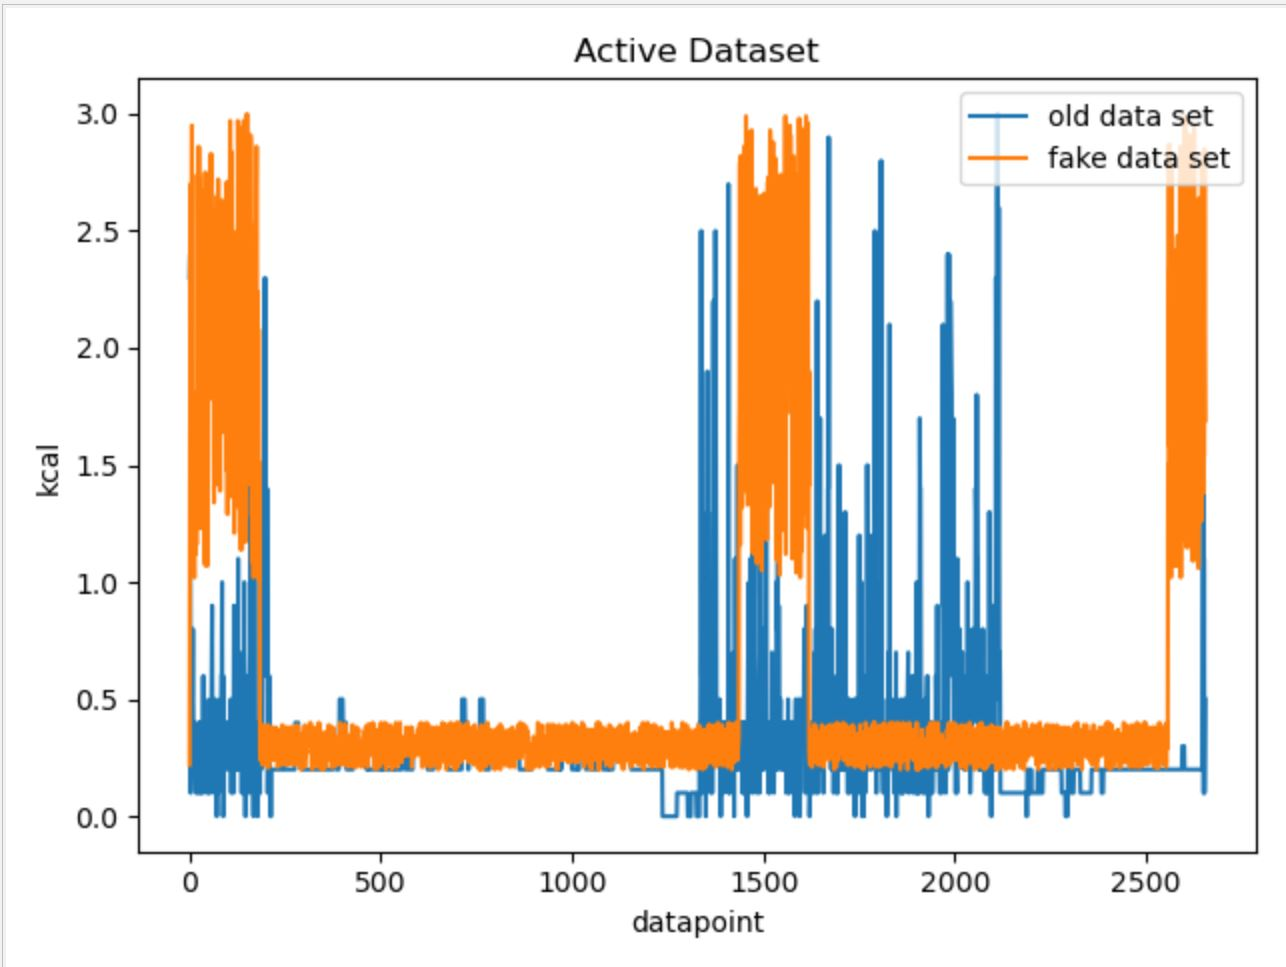
\includegraphics[width=0.50000\textwidth]{./images/Active Data.JPG}

For other data categories, we utilized similar approaches while ajusting
parameters and the possible range of random number generation based on
each data categories' own characteristics. Below are the fake data
vs.~real data comparison graphs for other data categories.

For basal data:\\
\includegraphics[width=0.50000\textwidth]{./images/BasalData.png} For
Dist data:\\
\includegraphics[width=0.50000\textwidth]{./images/Dist Data.JPG} For
Elev data:\\
\includegraphics[width=0.50000\textwidth]{./images/Elev Data.JPG} For
Heart data:\\
\includegraphics[width=0.50000\textwidth]{./images/Heart Data.JPG} For
Steps data:\\
\includegraphics[width=0.50000\textwidth]{./images/Steps Data.JPG}

\subsection{How to run the scripts?}\label{how-to-run-the-scripts}

In order to run the scripts, some modifications to the
GenerateFakeData.py are needed. There are three parameters that need
modification: folder\_name\_list, real\_name\_list, and path.
``folder\_name\_list'' tells the name of the folders that will contain
the dummy data. ``real\_name\_list'' tells the name of the reference
files being used to generate dummy data. ``path'' is the current
directory. Once these three parameters are set up correctly, just
directly run the GenerateFakeData.py script with no input.

\subsection{Potential improvements}\label{potential-improvements}

Because our dummy data generation script is specifically modified for
each data set, if in the future a new type of data appears, we need to
rewrite our code in order to accommodate the new data type. Therefore,
we can improve our code by applying more statictical knowledge so that
the code can be applied to generate dummy data from more different data
types.

\section{Creating a connection between API
Endpoints}\label{creating-a-connection-between-api-endpoints}

\subsection{List of API end-points:}\label{list-of-api-end-points}

\begin{enumerate}
\def\labelenumi{\arabic{enumi}.}
\tightlist
\item
  Front-End Patient User input to the database
\item
  Biometric Data from the FitBit API to the database
\item
  Data from the database to the RShiny Dashboard for visualization
\end{enumerate}

\subsection{What framework we are going to
use?}\label{what-framework-we-are-going-to-use}

We are currently looking to use the framework Express.js to write the
routes between the database and various API endpoints.

Express is a fast, light-weight web framework for Node.js. Express is a
pretty good framework. It's the most popular node application framework
out there. Express is widely used as middleware in node apps as it helps
to organize your app into a MVC architecture. It's the E of the popular
MEAN stack. Express manages following things very easily:

\begin{itemize}
\tightlist
\item
  Routing
\item
  Sessions
\item
  HTTP requests
\item
  Error handling
\end{itemize}

At times writing code from scratch for above things can be time
consuming. But by using express it's only a matter of few methods.
Express also helps in organizing your code.

\href{https://medium.com/@onejohi/building-a-simple-rest-api-with-nodejs-and-express-da6273ed7ca9}{Link
to set up Node}

\subsection{Setting up SQL database
connection:}\label{setting-up-sql-database-connection}

We created a connection with the MariaDB database in our Node Rest API
server to be able to send and receive data. The following link shows a
tutorial on how we set up the connection.

\href{https://bezkoder.com/node-js-rest-api-express-mysql/}{Link to
setup SQL connection in Node}

\subsection{Design of the Routes}\label{design-of-the-routes}

There are five kinds of routes:

\textbf{GET}: The GET method requests a representation of the specified
resource. Requests using GET should only retrieve data and should have
no other effect.

\textbf{POST}: The POST method requests that the server accept the
entity enclosed in the request as a new subordinate of the web resource
identified by the URI. The data POSTed might be, for example, an
annotation for existing resources; a message for a bulletin board,
newsgroup, mailing list, or comment thread; a block of data that is the
result of submitting a web form to a data-handling process; or an item
to add to a database.

\textbf{PUT}: The PUT method requests that the enclosed entity be stored
under the supplied URI. If the URI refers to an already existing
resource, it is modified; if the URI does not point to an existing
resource, then the server can create the resource with that URI.

\textbf{DELETE}: The DELETE method deletes the specified resource.

\textbf{PATCH}: The PATCH method applies partial modifications to a
resource

\section{Hosting the database on a
Server}\label{hosting-the-database-on-a-server}

\subsection{Issues faced with hosting a database on
Scholar:}\label{issues-faced-with-hosting-a-database-on-scholar}

\begin{enumerate}
\def\labelenumi{\arabic{enumi}.}
\tightlist
\item
  Scholar is a small computer cluster, suitable for classroom learning
  about high performance computing (HPC).
\item
  It can be accessed as a typical cluster, with a job scheduler
  distributing batch jobs onto its worker nodes, or as an interactive
  resource, with software packages available through a desktop-like
  environment on its login servers.
\item
  We tried to create a connection to the sql server hosted on this
  server from our local but we faced issues because there was a firewall
  preventing access to the database from a foreign server
\item
  We tried running our Backend API on scholar but we were unable to
  install NodeJS, MySQLWorkbench and other packages on the server
  without authorization.
\end{enumerate}

\subsection{Work around}\label{work-around}

\begin{enumerate}
\def\labelenumi{\arabic{enumi}.}
\item
  In order to install packages on scholar, we are expected to make
  requests to the administration with a list of all program lines to run
  in the form of a SLURM job.
\item
  The Simple Linux Utility for Resource Management (SLURM) is a system
  providing job scheduling and job management on compute clusters. With
  SLURM, a user requests resources and submits a job to a queue. The
  system will then take jobs from queues, allocate the necessary nodes,
  and execute them.
\item
  To submit work to a SLURM queue, you must first create a job
  submission file.
\end{enumerate}

More info can be found at the following link:
\href{https://www.rcac.purdue.edu/knowledge/weber/run/slurm}{SLURM Job}

\subsection{How we proceeded}\label{how-we-proceeded}

Since we have to make a request each time we have to install a package,
we decided to make just one request with a complete list of all
installation. As a result, we wanted to host a temporary database on AWS
that we can connect to and test on using our local machine.

We created a copy of the entire database on AWS with the following
credentials:

\begin{itemize}
\tightlist
\item
  Hostname: rnr56s6e2uk326pj.cbetxkdyhwsb.us-east-1.rds.amazonaws.com
\item
  Username: cb3i17t0aqn6a4ff
\item
  Password: e2l4k9zn24shcj42
\end{itemize}

\section{Adding data to the database}\label{adding-data-to-the-database}

\subsection{Adding a CSV to the
database}\label{adding-a-csv-to-the-database}

\begin{enumerate}
\def\labelenumi{\arabic{enumi}.}
\tightlist
\item
  The data engineering team had made a script that creates a CSV file
  with all the users FitBit data when they make a request to the API
\item
  We decided to make a python script to load this csv data onto the
  database we hosted on AWS.
\end{enumerate}

\subsection{POST information}\label{post-information}

\begin{enumerate}
\def\labelenumi{\arabic{enumi}.}
\item
  The JSON to add a datapoint to the database is as follows:

\begin{verbatim}
 obj = {'collection_date': row["Date"],
       'steps': row["Steps"],
       'floors_climbed': row["Floors Climbed"],
       'total_miles': row["Total Miles"],
       'lightly_active_miles': ["Lightly Active Miles"],
       'moderately_active_miles': row["Moderately Active Miles"],
       'very_active_miles': row["Very Active Miles"],
       'sedentary_minutes': row["Sedentary Minutes"],
       'lightly_active_minutes': row["Lightly Active Minutes"],
       'fairly_active_minutes': row["Fairly Active Minutes"],
       'very_active_minutes': row["Very Active Minutes"],
       'hr30_100_minutes': row["HR 30-100 Minutes"],
       'hr100_140_minutes': row["HR 100-140 Minutes"],
       'hr140_170_minutes': row["HR 140-170 Minutes"],
       'hr170_220_minutes': row["HR 170-220 Minutes"],
       'average_resting_heartrate': row["Average Resting HR"],
       'bmi': row["BMI"],
       'sleep_efficiency': row["Sleep Efficiency"],
       'weight': row["Weight"],
       'minutes_asleep': row["Minutes Alseep"],
       'fbusername': row["username"]
       }
\end{verbatim}
\item
  We made structures in this form by reading the CSV information into a
  pandas dataframe and made a post request to our API
\end{enumerate}

\subsection{Patient information and Study Specific
Data}\label{patient-information-and-study-specific-data}

The patient information is sent to the database form a webpage which
will be used by Merck Scientists to load the patients they are studying
during a clinical trial.

The JSON for a patient is as follows:

\begin{verbatim}
{
  patient_id,
  fbusername,
  first_name,
  last_name,
  gender,
  date_of_birth,
  height
}
\end{verbatim}

The JSON for the study data is as follows:

\begin{verbatim}
{
    patient_id,
    input_date,
    family_history_cancer,
    family_history_heart_disease,
    diagnostic_notes
}
\end{verbatim}

\section{Firebase and Login System for the Phone
App}\label{firebase-and-login-system-for-the-phone-app}

(This part is also in frontend team's documentation, because it is
relavant to both of the teams) Because our app's users are patients and
their information is very confidential, It is important to implement our
login and authentication system securely. Instead of building a secure
login system from scratch by ourselves, we chose to use a pre-existing
login authentication solution--firebase. In firebase, users' passwords
are first encrypted and then stored. Even if hackers successfully gain
access to firebase's database, they still would not know the passwords
because everything stored there is the encrypted version.

The next step is to incorporate the firebase login system into our own
database. Our current thought is that, once the user logs in through
firebase, they will receive a key from firebase. Then whenever they want
to modify or store data in our database, they send the key along with
every HTTP request. The backend would check the correctness of the key
and only allow accessibility if the key is correct.

\chapter{Front End Team}\label{front-end-team}

\section{Utilization of Third Party
Software}\label{utilization-of-third-party-software}

The sole third party software being used in our application is Firebase,
a Google based software designed for user authentication purposes. The
codes upon which this app is built are independently developed by our
team members. The data used to develop the app is Biometric data
collected currently only through Fitbit, though the goal is to expand
the collection capability to be able to obtain Apple Watch data as well.
This data is accessed through an external Merck API which is linked
through an SCTP request.

\section{Software Components}\label{software-components}

Our application has five main sections. The first section covers
everything prior to successful user login. This includes the login page
along with Firebase authentication. The second section is the home page
where users would be able to view displayed data pertaining to
themselves. The third section is a graphics page where graphs are
presented, informing users their health progress and their default
Fitbit data. The fourth section is the question response page where
users are guided to complete questionnaires for the purpose of data
collection beyond the default data collected by the wearable device. The
final section is the user setting page where users can view and edit
their information and settings; a log out option is also available
through this section.

\subsection{Pre-Login section}\label{pre-login-section}

The pre-login section has been mostly completed, however we are yet to
integrate the firebase completely within the page itself. The firebase
portion of this page has been created. This portion does not contain any
important functions besides the absolute base, standard functions
required by firebase to run. The login page aspect of this section has a
few important functions. For one, the entire app is stacked into a
function called Loginpage to make it harder for consumers to access. The
page runs similar to as expected. There's a space to enter a username
and password and a login button which gives a notification that you are
being logged in. TextInput and TouchableOpacity were both enabled to
allow popup notifications and username and password entry. For the
password entry, secureTextEntry was set to true, which turns the letters
into dots as they are typed.

\subsection{Home Page Section}\label{home-page-section}

The home page section is very simple; the current home page is where
basic data such as sleep, heart rate, etc would be presented in a clean
fashion as a summary. It is our goal to implement additional features to
this page along with an in depth description of user's data through the
graphics page.

\subsection{Question Response Section}\label{question-response-section}

The question response page collects data to further bolster the health
data collected by the users' wearables. It has many implemented
functionality to facilitate the data collection process, for example, it
displays information based on users' previous responses; This is done
using the constructor function. It also uses the onChangeText function
for the sake of clarity when the user selects a value. Ideally, a camera
feature will be made available on this page in the event that a user
wishes to upload an image to further elaborate on their health
conditions.

\subsection{User Setting Section}\label{user-setting-section}

Finally, There is the user information page which contains all of the
basic testing information and personal information that clinical trial
patient would preferably want to know, users can also log out through
this page if they so wishes. Ideally, this page would also bare a camera
feature which allow users to set a profile picture. Codes are stored in
a function creatively named Code, and consists of basic text and image
functions with one TouchableOpacity function so far to log the user out.

\chapter{Phone App Documentation}\label{phone-app-documentation}

Team members: Abhimanyu Agarwal, Xin Du, Anav Sharma

\section{1. How to Setup}\label{how-to-setup}

\textbf{Note: You will not be able to run the application until you
finish all the setup steps below. These steps make sure that your
frontend (React Native), backend (Node.js), and the two databases used
(Firebase and Amazon S3) are interconnected correctly. Note: A global
search of the word ``PUTYOURDATAHERE'' will help you find all the places
where you need to add your own config info. A more detailed instruction
is also presented below.}

Once you are in the root folder of the project repo, type ``npm start''
on the command line. The expo browser tool will open in your browser.
Then, you can choose to run the application on browser (as a website),
Android device, or Apple device. For the spring 2021 semester final
version, the code works best on an Android device (you can either use an
emulator or a real device), and it works mostly on website. We haven't
had a chance to test it on Apple device.

In order to configure the frontend to work with your firebase
authentication, correct credentials need to be put into ``config.js''
file located in /src/FireBase. To work with your Amazon S3, change the
AMAZON\_S3\_DOMAIN variable to your Amazon S3 URL in the env.json file.
The API\_DOMAIN url is the URL of your backend.

For the Node.js backend, the root folder is at
/backend/biometricBackend. Once you navigate there, you can type ``node
server.js'' to start the server on port 3000.

In order to configure the backend to work with your MySQL database,
correct credentials need to be put into ``db.config.js'' file located in
/backend/biometricBackend/app/config.

In order to configure the backend to work with your Amazon S3, correct
credentials need to be put into
/backend/biometricBackend/app/controllers/image.controller.js. Some
tutorials that might help you include
\url{https://medium.com/@otoloye/uploading-files-to-aws-s3-using-nodejs-multer-mongodb-and-postman-part-1-de790b8131d4}.

\section{2. Technologies Used}\label{technologies-used}

The phone application Frontend is built with React-native and Expo CLI.
Backend is supported by Firebase, AWS S3, mySQL and Node.js.

Firebase is used for login authentication. User's email and password are
stored in Firebase. Whenever the user wants to login, their provided
credentials are checked against the values stored in the Firebase. The
codes upon which this application is built are independently developed
by our team members. The data used to develop the application is
Biometric data collected currently only through Fitbit, though the goal
is to expand the collection capability to be able to obtain Apple Watch
data as well.

This data is accessed through an external Merck API which is linked
through an SCTP request. Our application's users are patients and their
information is very confidential, It is important to implement our login
and authentication system securely. Instead of building a secure login
system from scratch by ourselves, we chose to use a pre-existing login
authentication solution--firebase. In firebase, users' passwords are
first encrypted and then stored. Even if hackers successfully gain
access to firebase's database, they still would not know the passwords
because everything stored there is the encrypted version.

We use Amazon S3 to store all of our user and questionnaire images.
Unlike MySQL, Amazon S3 provides us with a ready-to-use file system that
is more efficient to store large data such as images.

We use MySQL to store all the data other than images. The data schema of
the two used tables for phone application are below:
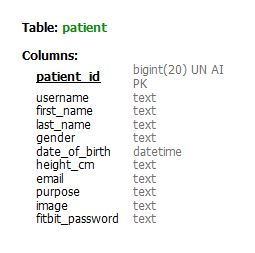
\includegraphics{./phone_app_doc_images/sql_patient_table.JPG}
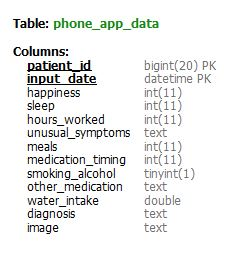
\includegraphics{./phone_app_doc_images/sql_phone_app_data_table.JPG}
Information related to the data schema used in our MySQL database is in
Data Architecture Team's document.

Besides, our main backend is Node.js. It is used to help the Frontend
communicate with the MySQL database. It also helps the frontend store
image to Amazon S3 instance.

\section{3. Application Description}\label{application-description}

The application is divided into 7 main pages. The description for each
page is listed below:

\subsection{3.1 Create Account Page}\label{create-account-page}

This page enables a user to build a new account by providing user
personal information. Information gathered from this Frontend is stored
using backend routes and models in mySQL database. One of the features
of this page is that it enables the user to upload an image. This image
is stored to Amazon S3 through Node.js. The Frontend would receive part
of the url (a number) that it can use to display the image.

For now, the image url is not stored into the database yet, although
it's stored in the frontend as a state variable. Once the user fills all
the inputs and click the button, all the data, along with the image url,
will be stored into the database (as a new row in the patient table). At
the same time, an user is created at firebase, which is later used for
authentication.

\begin{figure}
\centering
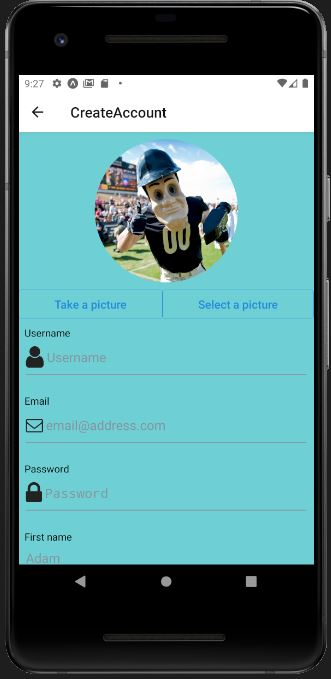
\includegraphics{./phone_app_doc_images/create_account_page.JPG}
\caption{}
\end{figure}

\subsection{3.2 Login Page}\label{login-page}

When user fills in the information and clicks the login button, the
following executions take place. First, the credentials are checked
against the Firebase authorisation data. Then, the credentials are also
used to retrieve the unique patient id from the SQL database, which is
used as the patient's identifier to grab corresponding data from the SQL
database.

\begin{figure}
\centering
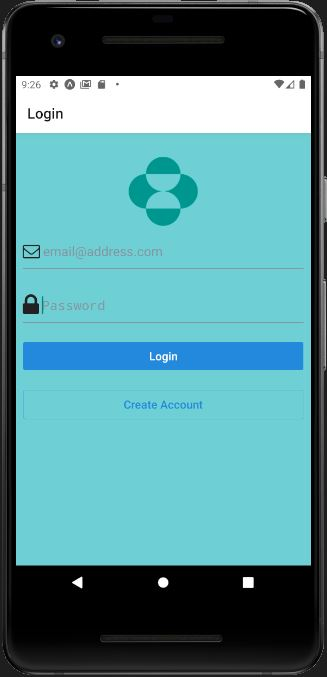
\includegraphics{./phone_app_doc_images/login_page.JPG}
\caption{}
\end{figure}

\subsection{3.3 Home Page}\label{home-page}

The Home Page provides the user to choose from multiple features of the
application. This page has a series of options that enable the user to
click pictures, upload pictures and also make new entries. While this
page does not explicitly communicate with the backend of the
application, it is crucial for full functioning of the application.

\begin{figure}
\centering
\includegraphics{./phone_app_doc_images/home_page.JPG}
\caption{}
\end{figure}

\subsection{3.4 Account Profile Page}\label{account-profile-page}

This page displays all the user corresponding information which is
fetched using the Patient id. This patient is instrumental to grab all
the corresponding information from the SQL database.

\begin{figure}
\centering
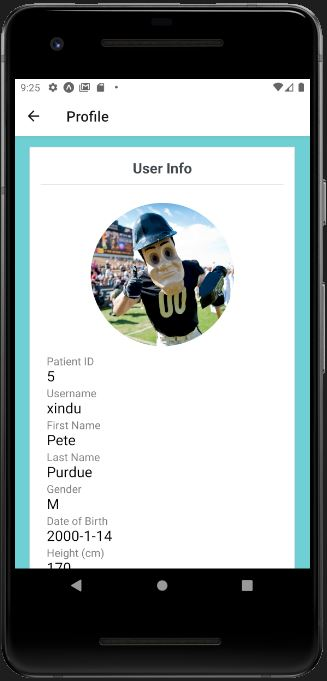
\includegraphics{./phone_app_doc_images/user_profile_page.JPG}
\caption{}
\end{figure}

\subsection{3.5 Edit Profile Page}\label{edit-profile-page}

Patient id is used to grab all the corresponding information from the
SQL database and the information is displayed. The user can also modify
the information and edit them in the SQL database. Once they edit it,
the new information will be pulled again and displayed on the page. This
page also enables the user to click picture and send it across for
further analysis. Along with the feature to click pictures, the user can
also upload images from local storage here.

\begin{figure}
\centering
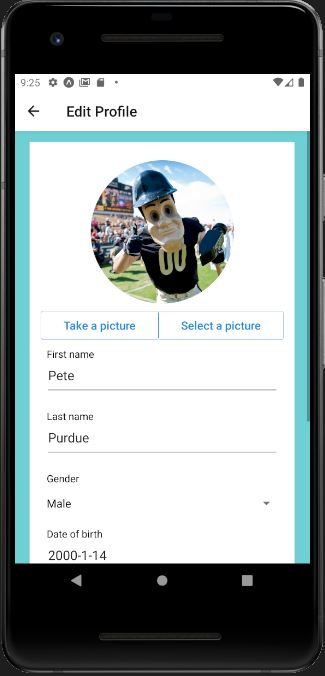
\includegraphics{./phone_app_doc_images/edit_profile_page.JPG}
\caption{}
\end{figure}

\subsection{3.6 Questionnaire Page}\label{questionnaire-page}

Consisting of series of questions, this page is used to create or edit a
new row in the phone\_app\_data table. If you enter this page from the
home page, you are going to execute a POST request, thus creating a new
row. If you enter this page from Entries page, you are going to execute
a PUT request, thus modifying an existing row. Once you click the
create/modify button, you will automatically go back to the home page.

\begin{figure}
\centering
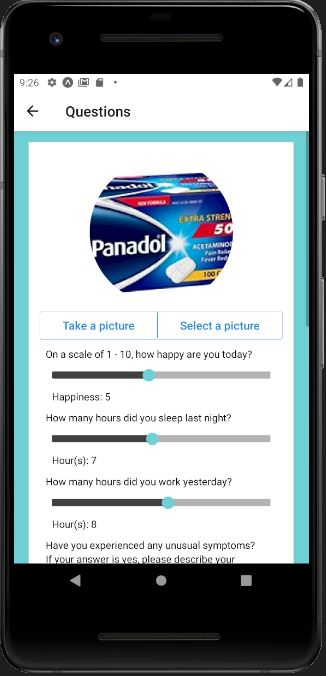
\includegraphics{./phone_app_doc_images/questionnaire_page.JPG}
\caption{}
\end{figure}

\subsection{3.7 Entries Page}\label{entries-page}

Displays the patient entry information. Each entry made by the user is
displayed. The data is fetched from all the rows with the current
patient id in the phone\_app\_data table.

\begin{figure}
\centering
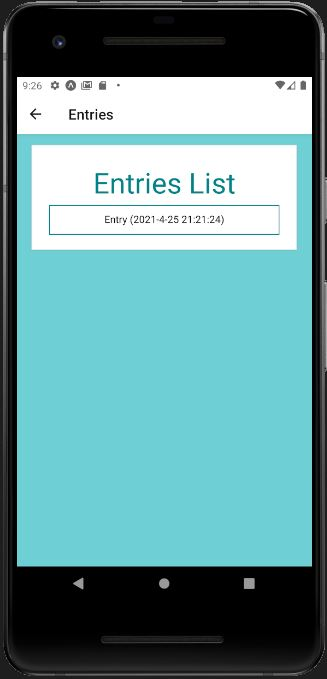
\includegraphics{./phone_app_doc_images/entries_page.JPG}
\caption{}
\end{figure}

\section{4. API endpoints (How Application's Frontend and Node.js
Backend
communicate)}\label{api-endpoints-how-applications-frontend-and-node.js-backend-communicate}

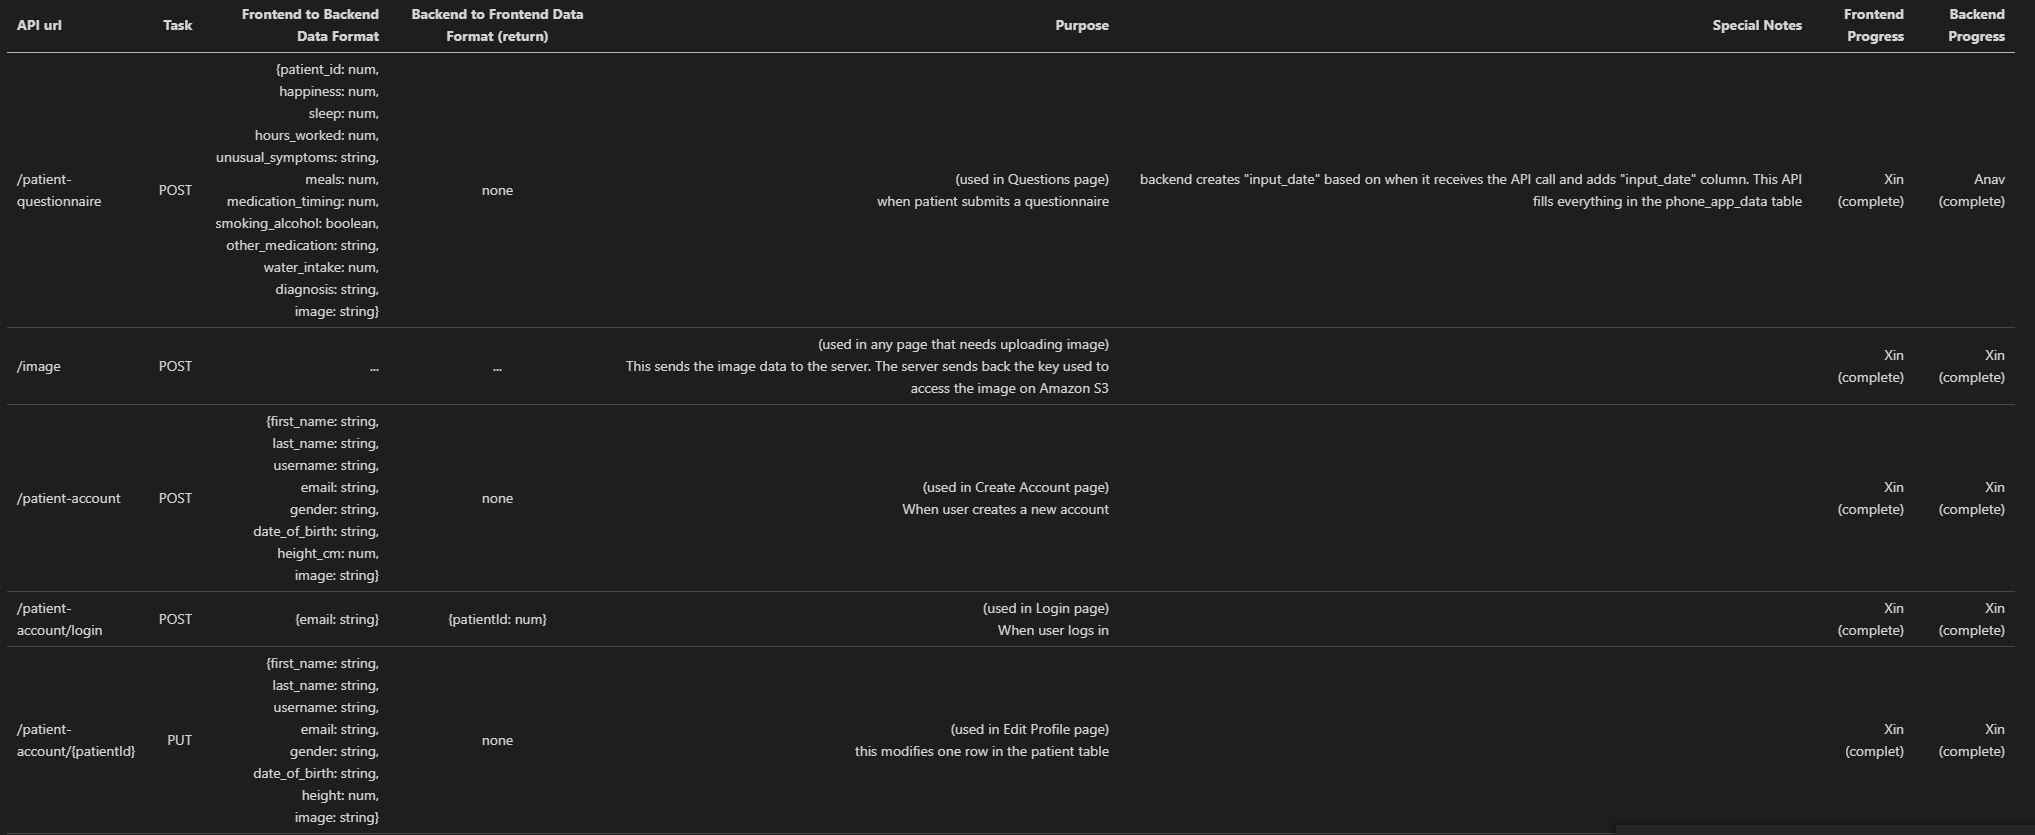
\includegraphics{./phone_app_doc_images/api_table_one.JPG}
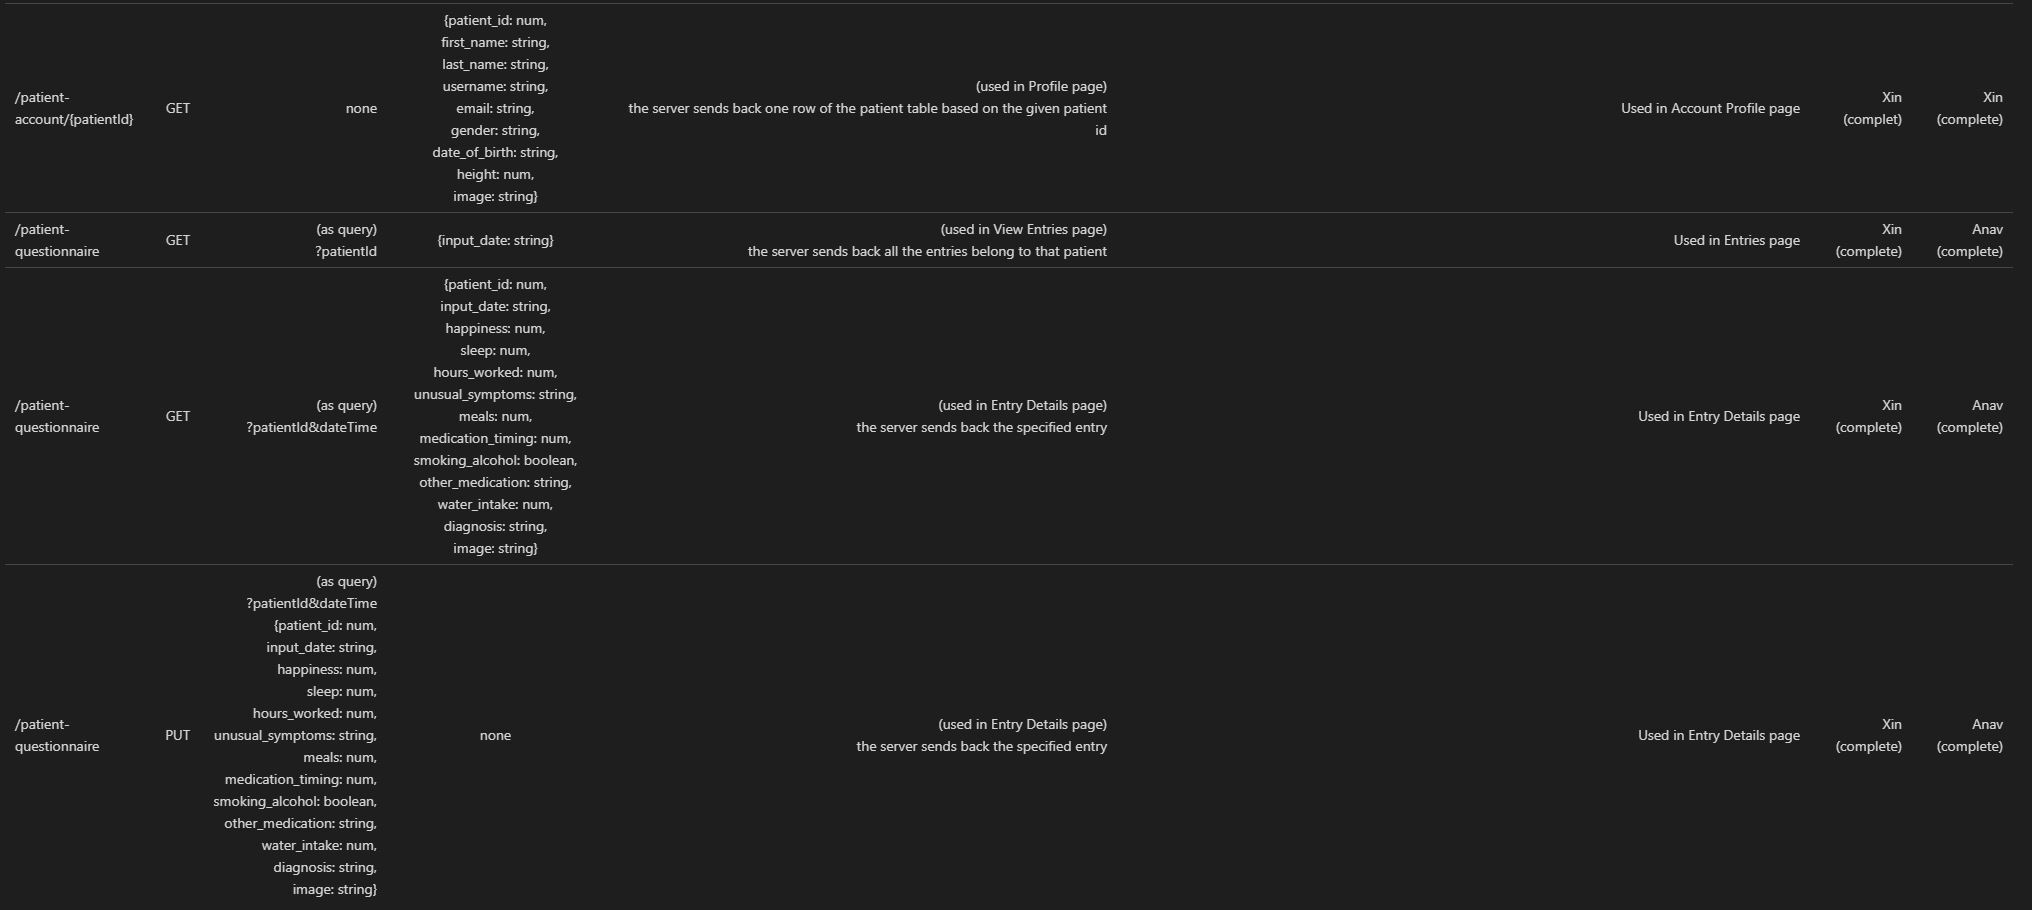
\includegraphics{./phone_app_doc_images/api_table_two.JPG}

\section{5. Future Work}\label{future-work-1}

\begin{enumerate}
\def\labelenumi{\arabic{enumi})}
\tightlist
\item
  We are planning to experiment using Xcode to develop an Apple version
  of the application.
\item
  We are planning to optimize the Front-end and add new features similar
  to click pictures, making new entries and uploading pictures.
\end{enumerate}

\section{6. Creation of Dummy Data}\label{creation-of-dummy-data-1}

\subsection{6.1 Why do we need dummy
data?}\label{why-do-we-need-dummy-data-1}

In order to effectively test the functionality of the backend code, a
lot of pre-existing data is needed to fill the database to simulate a
normal functioning environment for the app. Initially, we only had about
40 users' data, and it was not enough. Therefore, we decided to create
fake user data based on pre-existing user data (dummy data).

\subsection{6.2 How we generated dummy
data?}\label{how-we-generated-dummy-data-1}

In order to let dummy data make sense and follow pre-existing data's
patterns, we studied the patterns of each pre-existing data category.
There are active, basal, dist, elev, heart, and steps data. We mostly
used user 185 and 186's dataset as the reference while creating dummy
dataset.

For the active data, we first calculated the mean value of the original
data. Then we found out the number of data points above the mean.
Because it can be observed that within each active data set, data points
above the mean value cluster into three group, and one of them always
starts at the beginning. Therefore, we also chose the start as the
position of the first high value data cluster, and randomly chose
position for the other two. The value of each data point was chosen
based on the observed range of the reference data point.

The result of fake data vs.~real data graph can be found below:\\
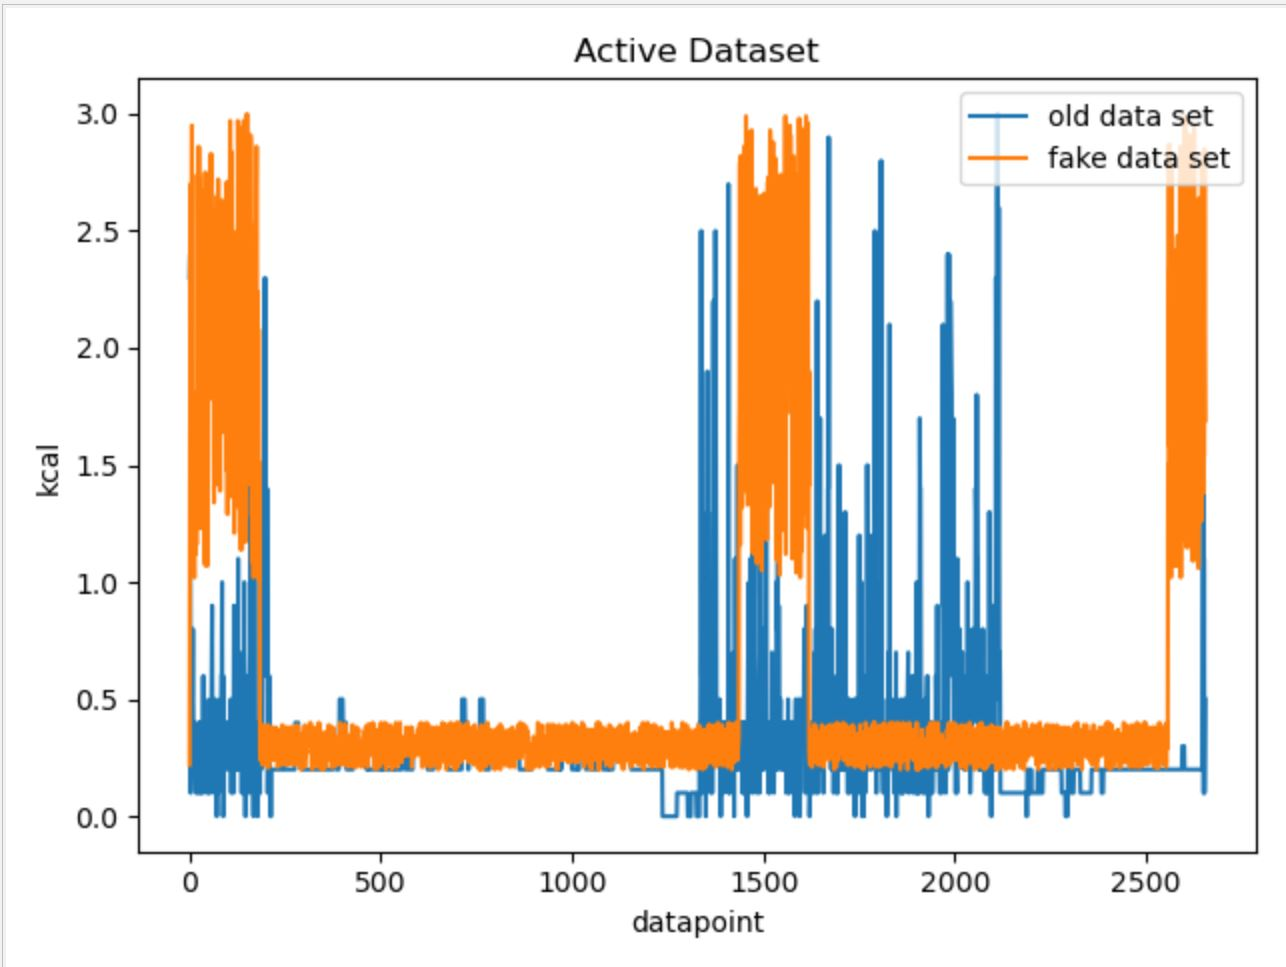
\includegraphics[width=0.50000\textwidth]{./images/Active Data.JPG}

For other data categories, we utilized similar approaches while ajusting
parameters and the possible range of random number generation based on
each data categories' own characteristics. Below are the fake data
vs.~real data comparison graphs for other data categories.

For basal data:\\
\includegraphics{./phone_app_doc_images/BasalData.png} For Dist data:\\
\includegraphics{./phone_app_doc_images/DistData.JPG} For Elev data:\\
\includegraphics{./phone_app_doc_images/ElevData.JPG} For Heart data:\\
\includegraphics{./phone_app_doc_images/HeartData.JPG} For Steps data:\\
\includegraphics{./phone_app_doc_images/StepsData.JPG}

\subsection{6.3 How to run the scripts?}\label{how-to-run-the-scripts-1}

In order to run the scripts, some modifications to the
GenerateFakeData.py are needed. There are three parameters that need
modification: folder\_name\_list, real\_name\_list, and path.
``folder\_name\_list'' tells the name of the folders that will contain
the dummy data. ``real\_name\_list'' tells the name of the reference
files being used to generate dummy data. ``path'' is the current
directory. Once these three parameters are set up correctly, just
directly run the GenerateFakeData.py script with no input.

\subsection{6.4 Potential improvements}\label{potential-improvements-1}

Because our dummy data generation script is specifically modified for
each data set, if in the future a new type of data appears, we need to
rewrite our code in order to accommodate the new data type. Therefore,
we can improve our code by applying more statictical knowledge so that
the code can be applied to generate dummy data from more different data
types.

\section{7. Creating a connection between API
Endpoints}\label{creating-a-connection-between-api-endpoints-1}

\subsection{7.1 List of API end-points:}\label{list-of-api-end-points-1}

\begin{enumerate}
\def\labelenumi{\arabic{enumi}.}
\tightlist
\item
  Front-End Patient User input to the database
\item
  Biometric Data from the FitBit API to the database
\item
  Data from the database to the RShiny Dashboard for visualization
\end{enumerate}

\subsection{7.2 What framework we are going to
use?}\label{what-framework-we-are-going-to-use-1}

We are currently looking to use the framework Express.js to write the
routes between the database and various API endpoints.

Express is a fast, light-weight web framework for Node.js. Express is a
pretty good framework. It's the most popular node application framework
out there. Express is widely used as middleware in node apps as it helps
to organize your app into a MVC architecture. It's the E of the popular
MEAN stack. Express manages following things very easily:

\begin{itemize}
\tightlist
\item
  Routing
\item
  Sessions
\item
  HTTP requests
\item
  Error handling
\end{itemize}

At times writing code from scratch for above things can be time
consuming. But by using express it's only a matter of few methods.
Express also helps in organizing your code.

\href{https://medium.com/@onejohi/building-a-simple-rest-api-with-nodejs-and-express-da6273ed7ca9}{Link
to set up Node}

\subsection{7.3 Setting up SQL database
connection:}\label{setting-up-sql-database-connection-1}

We created a connection with the MariaDB database in our Node Rest API
server to be able to send and receive data. The following link shows a
tutorial on how we set up the connection.

\href{https://bezkoder.com/node-js-rest-api-express-mysql/}{Link to
setup SQL connection in Node}

\subsection{7.4 Design of the Routes}\label{design-of-the-routes-1}

There are five kinds of routes:

\textbf{GET}: The GET method requests a representation of the specified
resource. Requests using GET should only retrieve data and should have
no other effect.

\textbf{POST}: The POST method requests that the server accept the
entity enclosed in the request as a new subordinate of the web resource
identified by the URI. The data POSTed might be, for example, an
annotation for existing resources; a message for a bulletin board,
newsgroup, mailing list, or comment thread; a block of data that is the
result of submitting a web form to a data-handling process; or an item
to add to a database.

\textbf{PUT}: The PUT method requests that the enclosed entity be stored
under the supplied URI. If the URI refers to an already existing
resource, it is modified; if the URI does not point to an existing
resource, then the server can create the resource with that URI.

\textbf{DELETE}: The DELETE method deletes the specified resource.

\textbf{PATCH}: The PATCH method applies partial modifications to a
resource

\section{8. Hosting the database on a
Server}\label{hosting-the-database-on-a-server-1}

\subsection{8.1 Issues faced with hosting a database on
Scholar:}\label{issues-faced-with-hosting-a-database-on-scholar-1}

\begin{enumerate}
\def\labelenumi{\arabic{enumi}.}
\tightlist
\item
  Scholar is a small computer cluster, suitable for classroom learning
  about high performance computing (HPC).
\item
  It can be accessed as a typical cluster, with a job scheduler
  distributing batch jobs onto its worker nodes, or as an interactive
  resource, with software packages available through a desktop-like
  environment on its login servers.
\item
  We tried to create a connection to the sql server hosted on this
  server from our local but we faced issues because there was a firewall
  preventing access to the database from a foreign server
\item
  We tried running our Backend API on scholar but we were unable to
  install NodeJS, MySQLWorkbench and other packages on the server
  without authorization.
\end{enumerate}

\subsection{8.2 Work around}\label{work-around-1}

\begin{enumerate}
\def\labelenumi{\arabic{enumi}.}
\item
  In order to install packages on scholar, we are expected to make
  requests to the administration with a list of all program lines to run
  in the form of a SLURM job.
\item
  The Simple Linux Utility for Resource Management (SLURM) is a system
  providing job scheduling and job management on compute clusters. With
  SLURM, a user requests resources and submits a job to a queue. The
  system will then take jobs from queues, allocate the necessary nodes,
  and execute them.
\item
  To submit work to a SLURM queue, you must first create a job
  submission file.
\end{enumerate}

More info can be found at the following link:
\href{https://www.rcac.purdue.edu/knowledge/weber/run/slurm}{SLURM Job}

\subsection{8.3 How we proceeded}\label{how-we-proceeded-1}

Since we have to make a request each time we have to install a package,
we decided to make just one request with a complete list of all
installation. As a result, we wanted to host a temporary database on AWS
that we can connect to and test on using our local machine.

We created a copy of the entire database on AWS with the following
credentials:

\begin{itemize}
\tightlist
\item
  Hostname: rnr56s6e2uk326pj.cbetxkdyhwsb.us-east-1.rds.amazonaws.com
\item
  Username: cb3i17t0aqn6a4ff
\item
  Password: e2l4k9zn24shcj42
\end{itemize}

\section{9. Adding data to the
database}\label{adding-data-to-the-database-1}

\subsection{9.1 Adding a CSV to the
database}\label{adding-a-csv-to-the-database-1}

\begin{enumerate}
\def\labelenumi{\arabic{enumi}.}
\tightlist
\item
  The data engineering team had made a script that creates a CSV file
  with all the users FitBit data when they make a request to the API
\item
  We decided to make a python script to load this csv data onto the
  database we hosted on AWS.
\end{enumerate}

\subsection{9.2 POST information}\label{post-information-1}

\begin{enumerate}
\def\labelenumi{\arabic{enumi}.}
\item
  The JSON to add a datapoint to the database is as follows:

\begin{verbatim}
 obj = {'collection_date': row["Date"],
       'steps': row["Steps"],
       'floors_climbed': row["Floors Climbed"],
       'total_miles': row["Total Miles"],
       'lightly_active_miles': ["Lightly Active Miles"],
       'moderately_active_miles': row["Moderately Active Miles"],
       'very_active_miles': row["Very Active Miles"],
       'sedentary_minutes': row["Sedentary Minutes"],
       'lightly_active_minutes': row["Lightly Active Minutes"],
       'fairly_active_minutes': row["Fairly Active Minutes"],
       'very_active_minutes': row["Very Active Minutes"],
       'hr30_100_minutes': row["HR 30-100 Minutes"],
       'hr100_140_minutes': row["HR 100-140 Minutes"],
       'hr140_170_minutes': row["HR 140-170 Minutes"],
       'hr170_220_minutes': row["HR 170-220 Minutes"],
       'average_resting_heartrate': row["Average Resting HR"],
       'bmi': row["BMI"],
       'sleep_efficiency': row["Sleep Efficiency"],
       'weight': row["Weight"],
       'minutes_asleep': row["Minutes Alseep"],
       'fbusername': row["username"]
       }
\end{verbatim}
\item
  We made structures in this form by reading the CSV information into a
  pandas dataframe and made a post request to our API
\end{enumerate}

\subsection{9.3 Patient information and Study Specific
Data}\label{patient-information-and-study-specific-data-1}

The patient information is sent to the database form a webpage which
will be used by Merck Scientists to load the patients they are studying
during a clinical trial.

The JSON for a patient is as follows:

\begin{verbatim}
{
  patient_id,
  fbusername,
  first_name,
  last_name,
  gender,
  date_of_birth,
  height
}
\end{verbatim}

The JSON for the study data is as follows:

\begin{verbatim}
{
    patient_id,
    input_date,
    family_history_cancer,
    family_history_heart_disease,
    diagnostic_notes
}
\end{verbatim}

\chapter{Fullstack Documentation Spring
2021}\label{fullstack-documentation-spring-2021}

Fall 2020 Semester Back End Documentation can be found at :
\url{https://nicholasrosenorn.github.io/BiometricsDocumentation/back-end-team.html}

Fall 2020 Semester Front End Documentation can be found at:
\url{https://nicholasrosenorn.github.io/BiometricsDocumentation/front-end-team.html}

\section{Sprint 1 (01/19 - 02/15)}\label{sprint-1-0119---0215}

During this sprint we spent time planning and designing the UI and
working parts of our projects.

The following are pdfs of sketches of our overall project, the user
pages for our mobile application and the pages for our website. The pdfs
also layout the technologies we are using to build our application as
well as the services we are using to host our database.

\begin{figure}
\centering
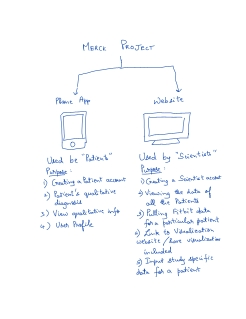
\includegraphics{images/project_overview.png}
\caption{}
\end{figure}

\begin{figure}
\centering
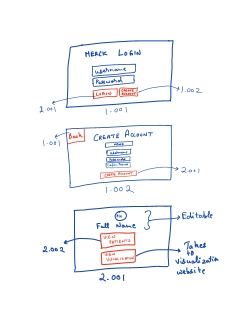
\includegraphics{images/page1_001.jpg}
\caption{}
\end{figure}

Below is how we plan to divide the work:

\subsection{Website:}\label{website}

Connor: Login page and create account

Patricia: Starter page and patients list

Sid: info and entry page

\subsection{Phone App:}\label{phone-app}

Anav: Login page and create account

Xin: Home page, info page , questions page

Abhi: list of entries, edit info, answers to an old entry (last page in
the sketches)

\subsection{Website Progress:}\label{website-progress}

Several templates found:

\url{https://bootsnipp.com/snippets/K0ZmK}

\url{https://bootsnipp.com/snippets/7nk08}

\url{https://bootsnipp.com/snippets/AlZ7g}

Sign up and sign in pages are complete. Currently connected to Firebase
authentication, however, after several hours of trying, we have
concluded that using Firebase for authentication is not ideal, and using
the built-in Flask authentication methods will be better. The only
Firebase library for Python is only for handling administration of the
Firebase Auth datatbase. Sessions are more complicated than first
anticipated. Accounts can currently be created using an email and
password, and these inputs are stored in a database. Currently working
on building a unifying layout.html to standardize the layout of all
pages on the website. This will allow for pages to seem connected
aesthetically and will allow for ease of page creation in the future.
The same will be done for a standard CSS file.

\subsection{Phone App Progress:}\label{phone-app-progress}

We also started finding already-made templates for both the webpage and
phone app.

For the phone app, we found a very good react native UI library: React
Native Elements

Several templates found:

\url{https://market.nativebase.io/view/react-native-delivery-app}

\section{Sprint 2 (02/16 - 03/01)}\label{sprint-2-0216---0301}

\subsection{Website Progress:}\label{website-progress-1}

Siddharth has completed the template for the patient view website. A
demo is found here: !

The next steps are to connect the website to the database and make GET
and POST requests to display patient information.

\subsection{Phone App Progress:}\label{phone-app-progress-1}

During the first week (02/16-2/22), several tasks have been
accomplished:

Investigate in firestore security rule and fix the bug of not being able
to login Build our project into an apk. and be able to run it on android

\begin{figure}
\centering
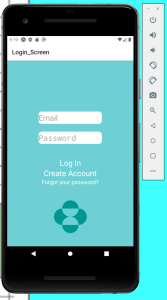
\includegraphics{images/mobile_signin.png}
\caption{}
\end{figure}

The second accomplishment is especially meaningful because this is the
issue that we have been facing since last semester. This accomplishment
means that we will be sure that our app will be capable of running on a
real Android device, and the camera functionality will be added
accordingly.

During the second week (02/22-3/01), we will add three more pages into
our app. They are:

Complete page 2.005 (edit profile page). Assigned to Ahbi Complete page
2.004 (View Entries Page). Assigned to Anav Complete Page 2.002 (User
Information Page). Assigned to Xin Meaning while, Ahbi and Xin are
working on the camera functionality.

\section{Sprint 3 (03/01 - 03/14)}\label{sprint-3-0301---0314}

\subsection{Website Progress:}\label{website-progress-2}

Siddharth: Completed the structure for the front end of the website.
Connections to the database need to be made to make the data actively
pull and post data to the database.

Completed the connections to the database and combined all the pages
created by the members. Added functionality to view and edit old
scientist notes as well as make a new note. Improved the theme for the
profiles page and fixed the issue with missing data.

\subsection{Phone App Progress so far:}\label{phone-app-progress-so-far}

Xin is working on page 2.002. The page 2.002's prototype has been
completed. The next stage is to make it look better.

Prototype:

\begin{figure}
\centering
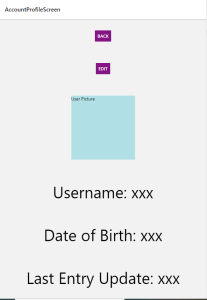
\includegraphics{images/mobile_prototype.png}
\caption{}
\end{figure}

Ahbi is still working on page 2.005, and Anav is still working on page
2.004.

Besides, we have reached a conclusion on how to store user images in our
database. We are planning to store references of images in our SQL
database. The references will point to a special database or filesystem
that actually stores all the images. By doing this, our SQL database
will not become too big and slow due to the large size of images. We
will investigate more on this in sprint 3.

On 3/8, we finished all the frontend pages of the phone app. Between 3/8
- 3/14, we will start working on the backend routes for the phone app to
connect it to the database.

\section{Sprint 3 (03/15 - 03/29)}\label{sprint-3-0315---0329}

\subsection{Website Progress so far:}\label{website-progress-so-far}

The website has been completed along with the image functionality as
well as created the demos for the Symposium video.

This week we will be working on deploying the app on an AWS EC2 instance
and linking the website to the visualizations dashboard.

\subsection{Phone App Progress so
far:}\label{phone-app-progress-so-far-1}

From 3/15 to 3/22, Abhi finished the code for uploading images from
phone's local storage and also using camera to take pictures. Then, Xin
worked on building backend routes and Amazon S3 instance to enable
storing images in our database. Xin also worked on rebuilding the UI of
the phone app to make it look better.

The details of these functionalities are demoed in the draft demo video.

\section{Sprint 4 (03/30 - 04/12)}\label{sprint-4-0330---0412}

\subsection{Website:}\label{website-1}

Sid: Created the configuration and set up to connect to an AWS S3 Bucket
and worked on cleaning the codebase

Connor: Worked on creating the animation for a CRON job and Fitbit data
flow into the database

\subsection{Phone App:}\label{phone-app-1}

Xin: Created a table of all the backend routes used by the Node Rest API
server

\section{Website design}\label{website-design}

\subsection{Choosing a Framework}\label{choosing-a-framework}

There are a seemingly endless number of options of web frameworks one
could use to build a website from scratch. To narrow down the search of
what framework to use, our team selected to use one designed for Python.
Python is one of the easier languages to learn and implement. It is
readable and is very well documented. On top of that, Python is the
language we are most comfortable with, which allowed us to focus on
building the project rather than learning a new programming language.
There are several packages designed for web frameworks in Python. Django
and Flask are by far the most popular and widely-used packages. They are
both free to use and open-source with plenty of additional packages
built by the community to ease the development process. After some
deliberation and experimentation, Flask was chosen because it is simpler
and easier to make small applications than Django.

Flask applications typically follow the same structure- an
initialization file (\textbf{init}.py), a routes file (routes.py), a
forms file (forms.py), and a models file (models.py).

\subsection{Scripts Explained}\label{scripts-explained}

\subsubsection{Initialization}\label{initialization}

This file will set up the Flask application, along with every other
application the website will utilize. For our website, this means Flask,
SQLAlchemy, Flask bcrypt, and Flask Login will all need to be
instantiated as part of the Flask application.

SQLAlchemy is how our application interfaces with our SQL database.
Flask Bcrypt is a Flask extension that provides bcrypt hashing
utilities. Bcrypt is a password-hashing function, which we use to hash
user passwords before storing them in the database. Flask Login is a
Flask extension that provides user session management. It handles
logging in, logging out, and user sessions. Forms

\subsubsection{Forms}\label{forms}

Forms in Flask are handled by FlaskForm, which is from the Flask-WTF
package. It offers an easy way to collect input data from a user because
it interfaces with HTML scripts seamlessly. To create a form, simply
define a class with the name of the form that inherits from FlaskForm.
Then define each input with a variable name. Each of these variables
will have a type of field that Flask-WTF defines. The most used ones
include StringField, DateField, TextAreaField, and SubmitField. Each of
these instances of an input field have the option for validators,
meaning when the form is submitted, the data will be tested based on the
validator to determine if the input field contains valid information.
For example, if a form contains an input for email, a Flask-WTF provided
validator that should be used is Email(), which will check to make sure
there is a valid email (meaning it contains an \citet{website.com} or
\citet{website.org}, etc.).

Custom validators can be made as well but are a little more complicated.
After each input field is defined, a function is created that passes the
variable name of the input field into it, and the logic that should be
applied to the contents of the field is applied. Custom validation error
strings can be raised, and these can be displayed with some formatting
in the HTML script associated with the page the form is on. No other
logic should be contained in the forms class. Other logic, such as
validating a log in, should be included in the route function for the
page.

\subsubsection{Models}\label{models}

Models are only necessary if the website will be sending data to a
database. For our website, we are using SQLAlchemy, but other packages
that handle the connections between the framework and the database may
have different requirements/syntax for models. A model class inherits
from the Model class from SQLAlchemy, and the name MUST be the SAME as
the table name of the database in which the data should be placed. If
the name of the table in the database is ``patient'', the name of the
class must be ``patient''. This same convention goes for the columns of
the database as well. To create a Column instance which correlates with
(and will place data into) a column within the table, the variable name
must be the same as the column name in the table. The Column class from
SQLAlchemy has the same parameters as SQL. For example, Booleans
primary\_key, unique, and nullable are all parameters that can define a
column. Think of these models as describing and mapping (Python to SQL)
the SQL database in which data should be placed.

\subsubsection{Routes}\label{routes}

Now that Flask models and forms have been explained, we can move on to
the routes. Flask routes are comprised of a function with the decorator
\citet{app.route}(``/route''). A route maps a specific URL to a function
that performs tasks such as storing data to a database or handling
events on the webpage. If the webpage contains data that is not static
(meaning data that will be passed in to or retrieved from the webpage),
``GET'' and ``POST'' methods must be added as parameters to the
decorator. For pages that require a valid login from a user in order to
access the page, the decorator \citet{login_required} from Flask Login
must be used.

Once the decorators have been added, the design of the route can begin.
Static webpages are fairly simple:

\begin{Shaded}
\begin{Highlighting}[]
\AttributeTok{@app.route}\NormalTok{(“}\OperatorTok{/}\NormalTok{home”)}
\KeywordTok{def}\NormalTok{ home():}
\ControlFlowTok{return}\NormalTok{ render_template(“welcome_page.html”)}
\end{Highlighting}
\end{Shaded}

This will load the HTML page ``welcome\_page.html'' when the route
entered is ``website.com/home'', where website.com is whatever the
website's name is.

The next step would be to incorporate the forms we previously discussed.
Let us walk through the example below. First, the function is defined
and the route decorator is added. Second, the form is instantiated.
Next, it is determined if the form was submitted and more importantly,
if it was valid when submitted. Then the model of the table the data
from the form should be placed in is instantiated, with the parameters
being data taken from the input form and passed to the column name of
the table. Finally, the current session has to be added to the database
and committed. The first return statement places the user back at the
home page once the form has been validated and submitted. The second
return statement will display the HTML page of the form.

\begin{Shaded}
\begin{Highlighting}[]
\AttributeTok{@app.route}\NormalTok{(“}\OperatorTok{/}\NormalTok{example_form”)}
\KeywordTok{def}\NormalTok{ example_form():}
\NormalTok{form }\OperatorTok{=}\NormalTok{ Form_Name()}
\ControlFlowTok{if}\NormalTok{ form.validate_on_submit():}
\NormalTok{              database_model }\OperatorTok{=}\NormalTok{ model(input_field_to_database}\OperatorTok{=}\NormalTok{form.input_field_from_form.data)}
\NormalTok{              db.session.add(database_model)}
\NormalTok{              db.session.commit()}
              \ControlFlowTok{return}\NormalTok{ redirect(url_for(‘home’))}
\ControlFlowTok{return}\NormalTok{ render_template(‘example_form.html’, title}\OperatorTok{=}\NormalTok{’Example Form’, form}\OperatorTok{=}\NormalTok{form)}
\end{Highlighting}
\end{Shaded}

\subsubsection{Description of Pages}\label{description-of-pages}

\paragraph{Create Account}\label{create-account}

The create account page is straightforward- you can either enter
credentials to create an account (which have to meet certain
requirements, email has to be valid, password must match with confirm
password and be longer than 6 characters), or redirect to the sign in
page.

\begin{figure}
\centering
\includegraphics{images/Create_account_page.png}
\caption{}
\end{figure}

\paragraph{Sign In}\label{sign-in}

This page gets redirected to after logging out and when trying to access
other routes without logging in. From here, one can sign in, redirect to
the create account page, or request a password change (which has not
been implemented yet).

\begin{figure}
\centering
\includegraphics{images/Sign_in_page.png}
\caption{}
\end{figure}

\paragraph{Home}\label{home}

This is the first thing users see after signing in. This page gives
access to the patient gallery and the visualizations dashboard. On this
page and every other page requiring a sign in, users can edit their
account or logout via the navbar on top. Clicking the company logo on
the left side of the navbar will redirect to this home page.

\begin{figure}
\centering
\includegraphics{images/home_page.png}
\caption{}
\end{figure}

\paragraph{Edit Account}\label{edit-account}

Scientists can update their email and change their password whenever
they need to. A given email can only be used by one account.

\begin{figure}
\centering
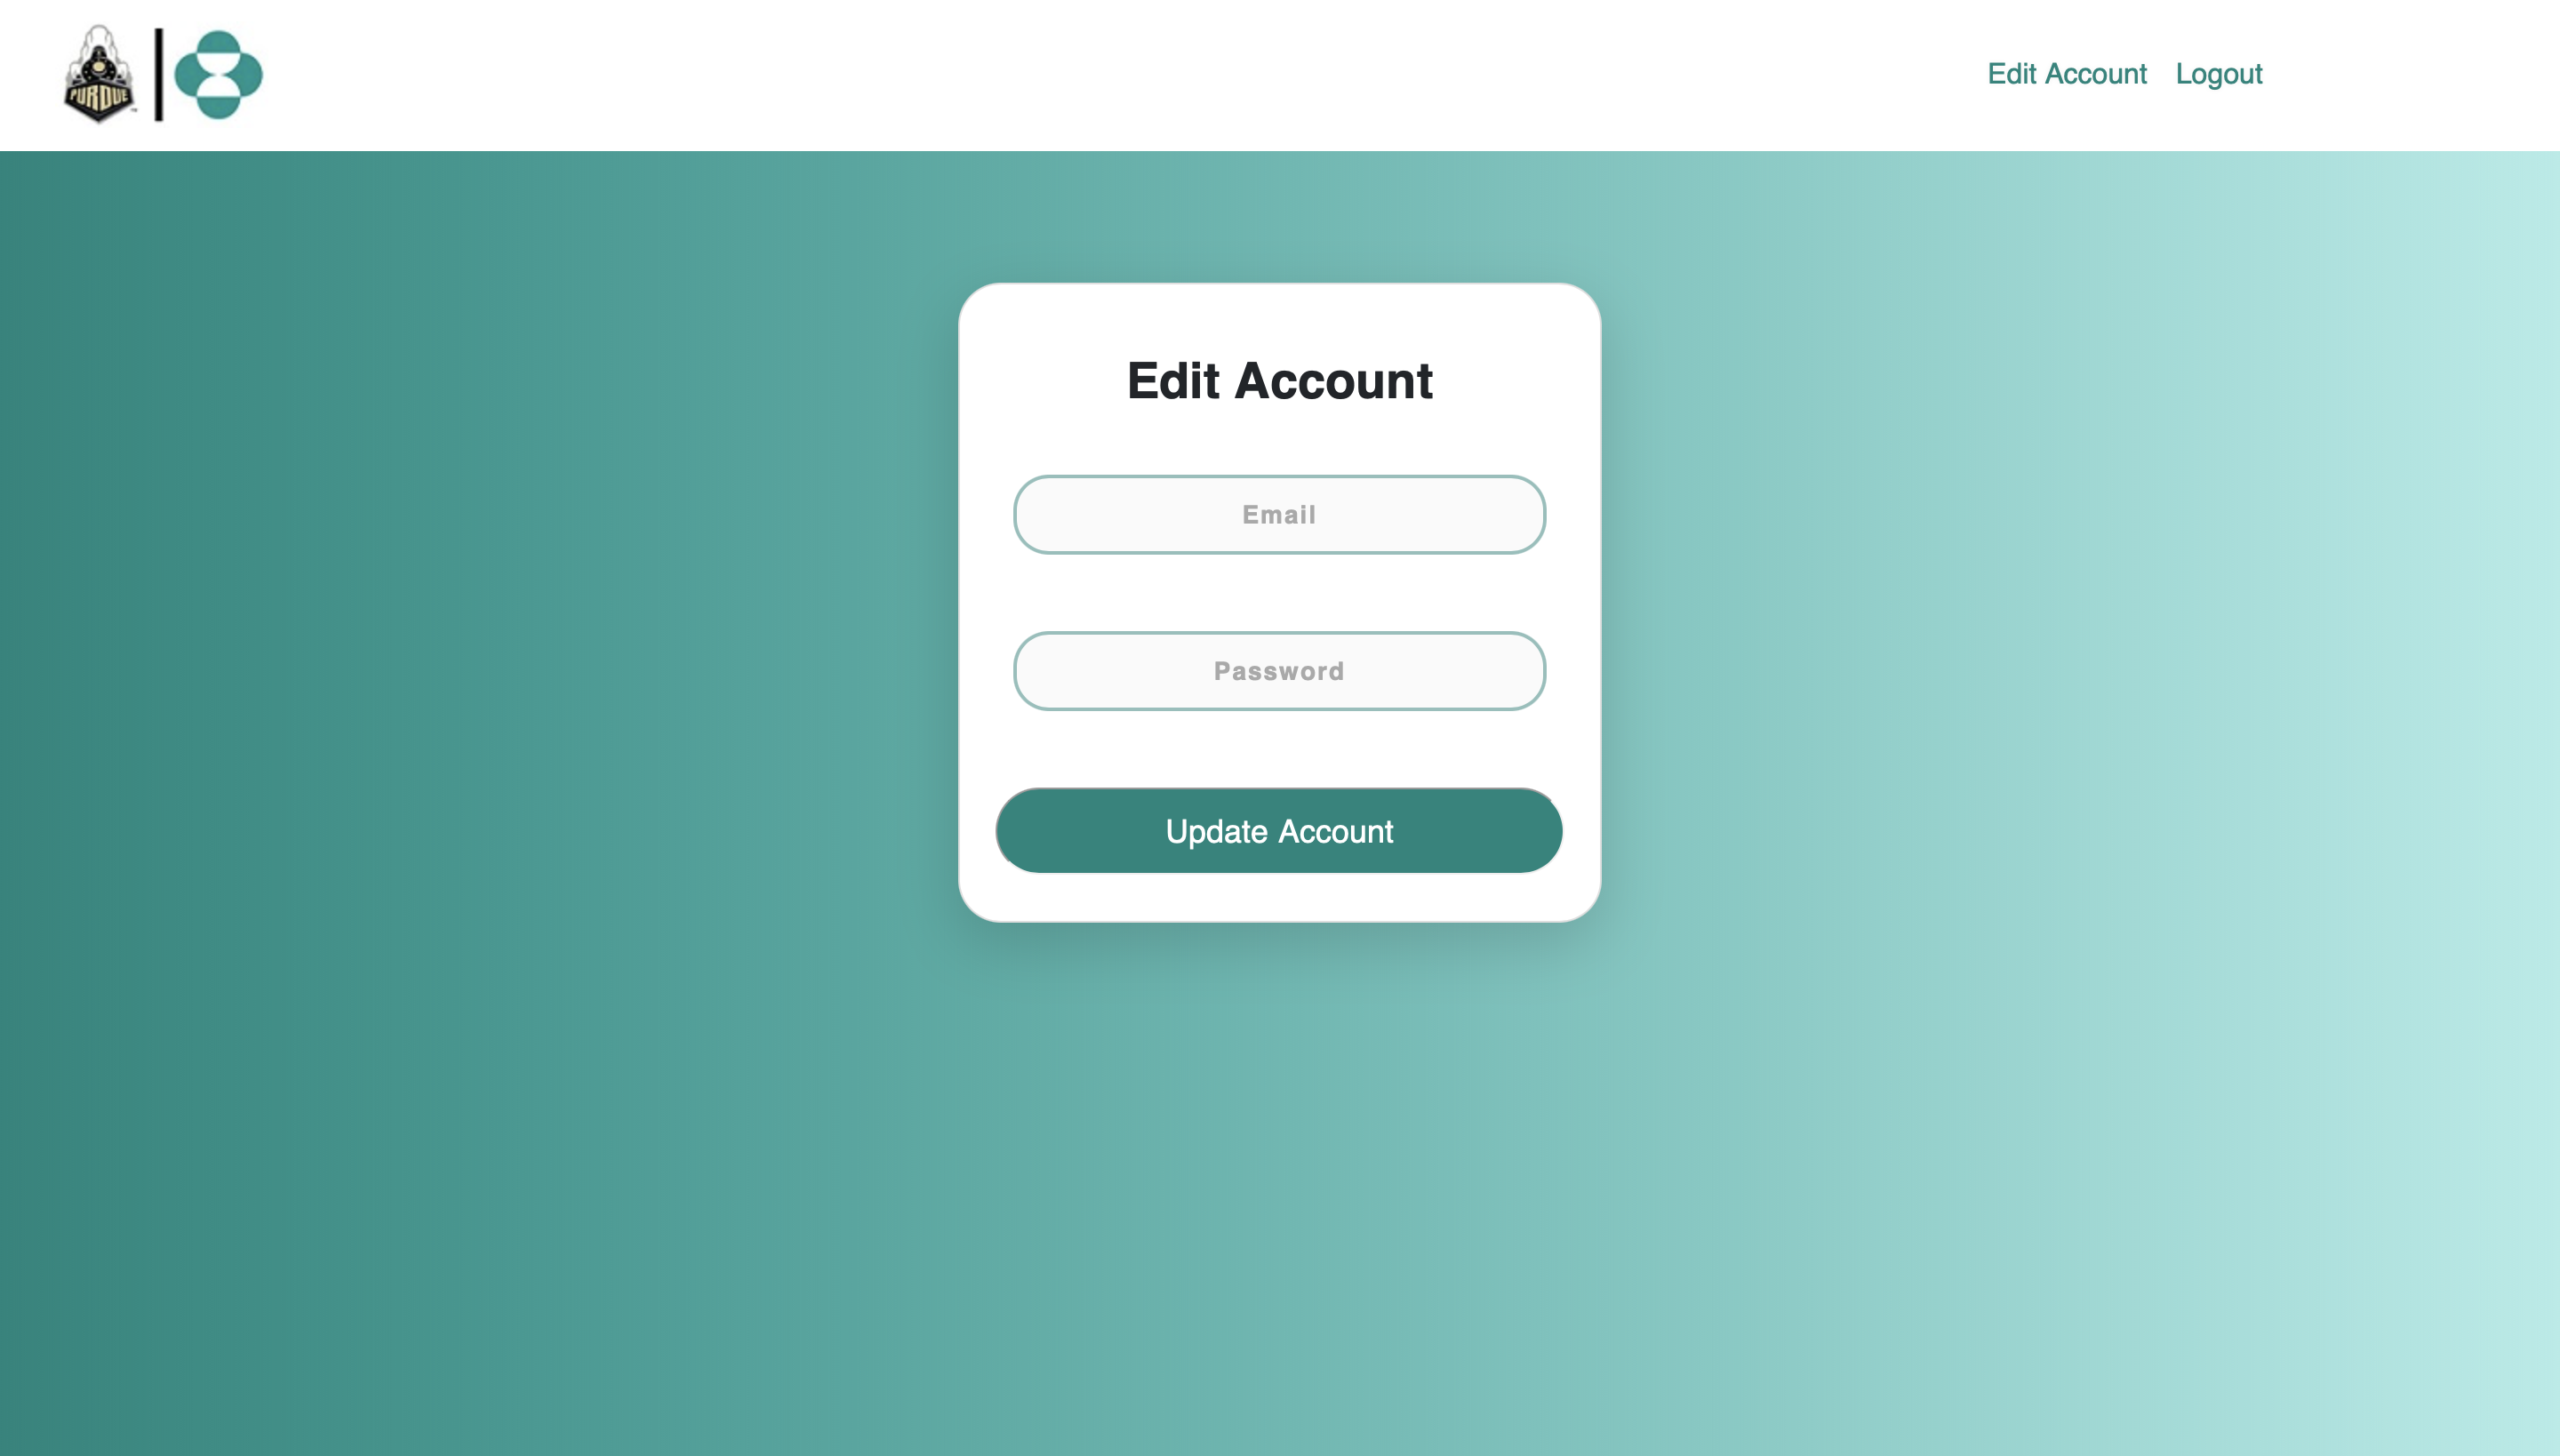
\includegraphics{images/Edit_Account.png}
\caption{}
\end{figure}

\paragraph{Patient Gallery}\label{patient-gallery}

All patients enrolled in the study are shown on this page with an image
and the study they are enrolled in. Features to sort by name, study, and
date enrolled will be part of future work.

\begin{figure}
\centering
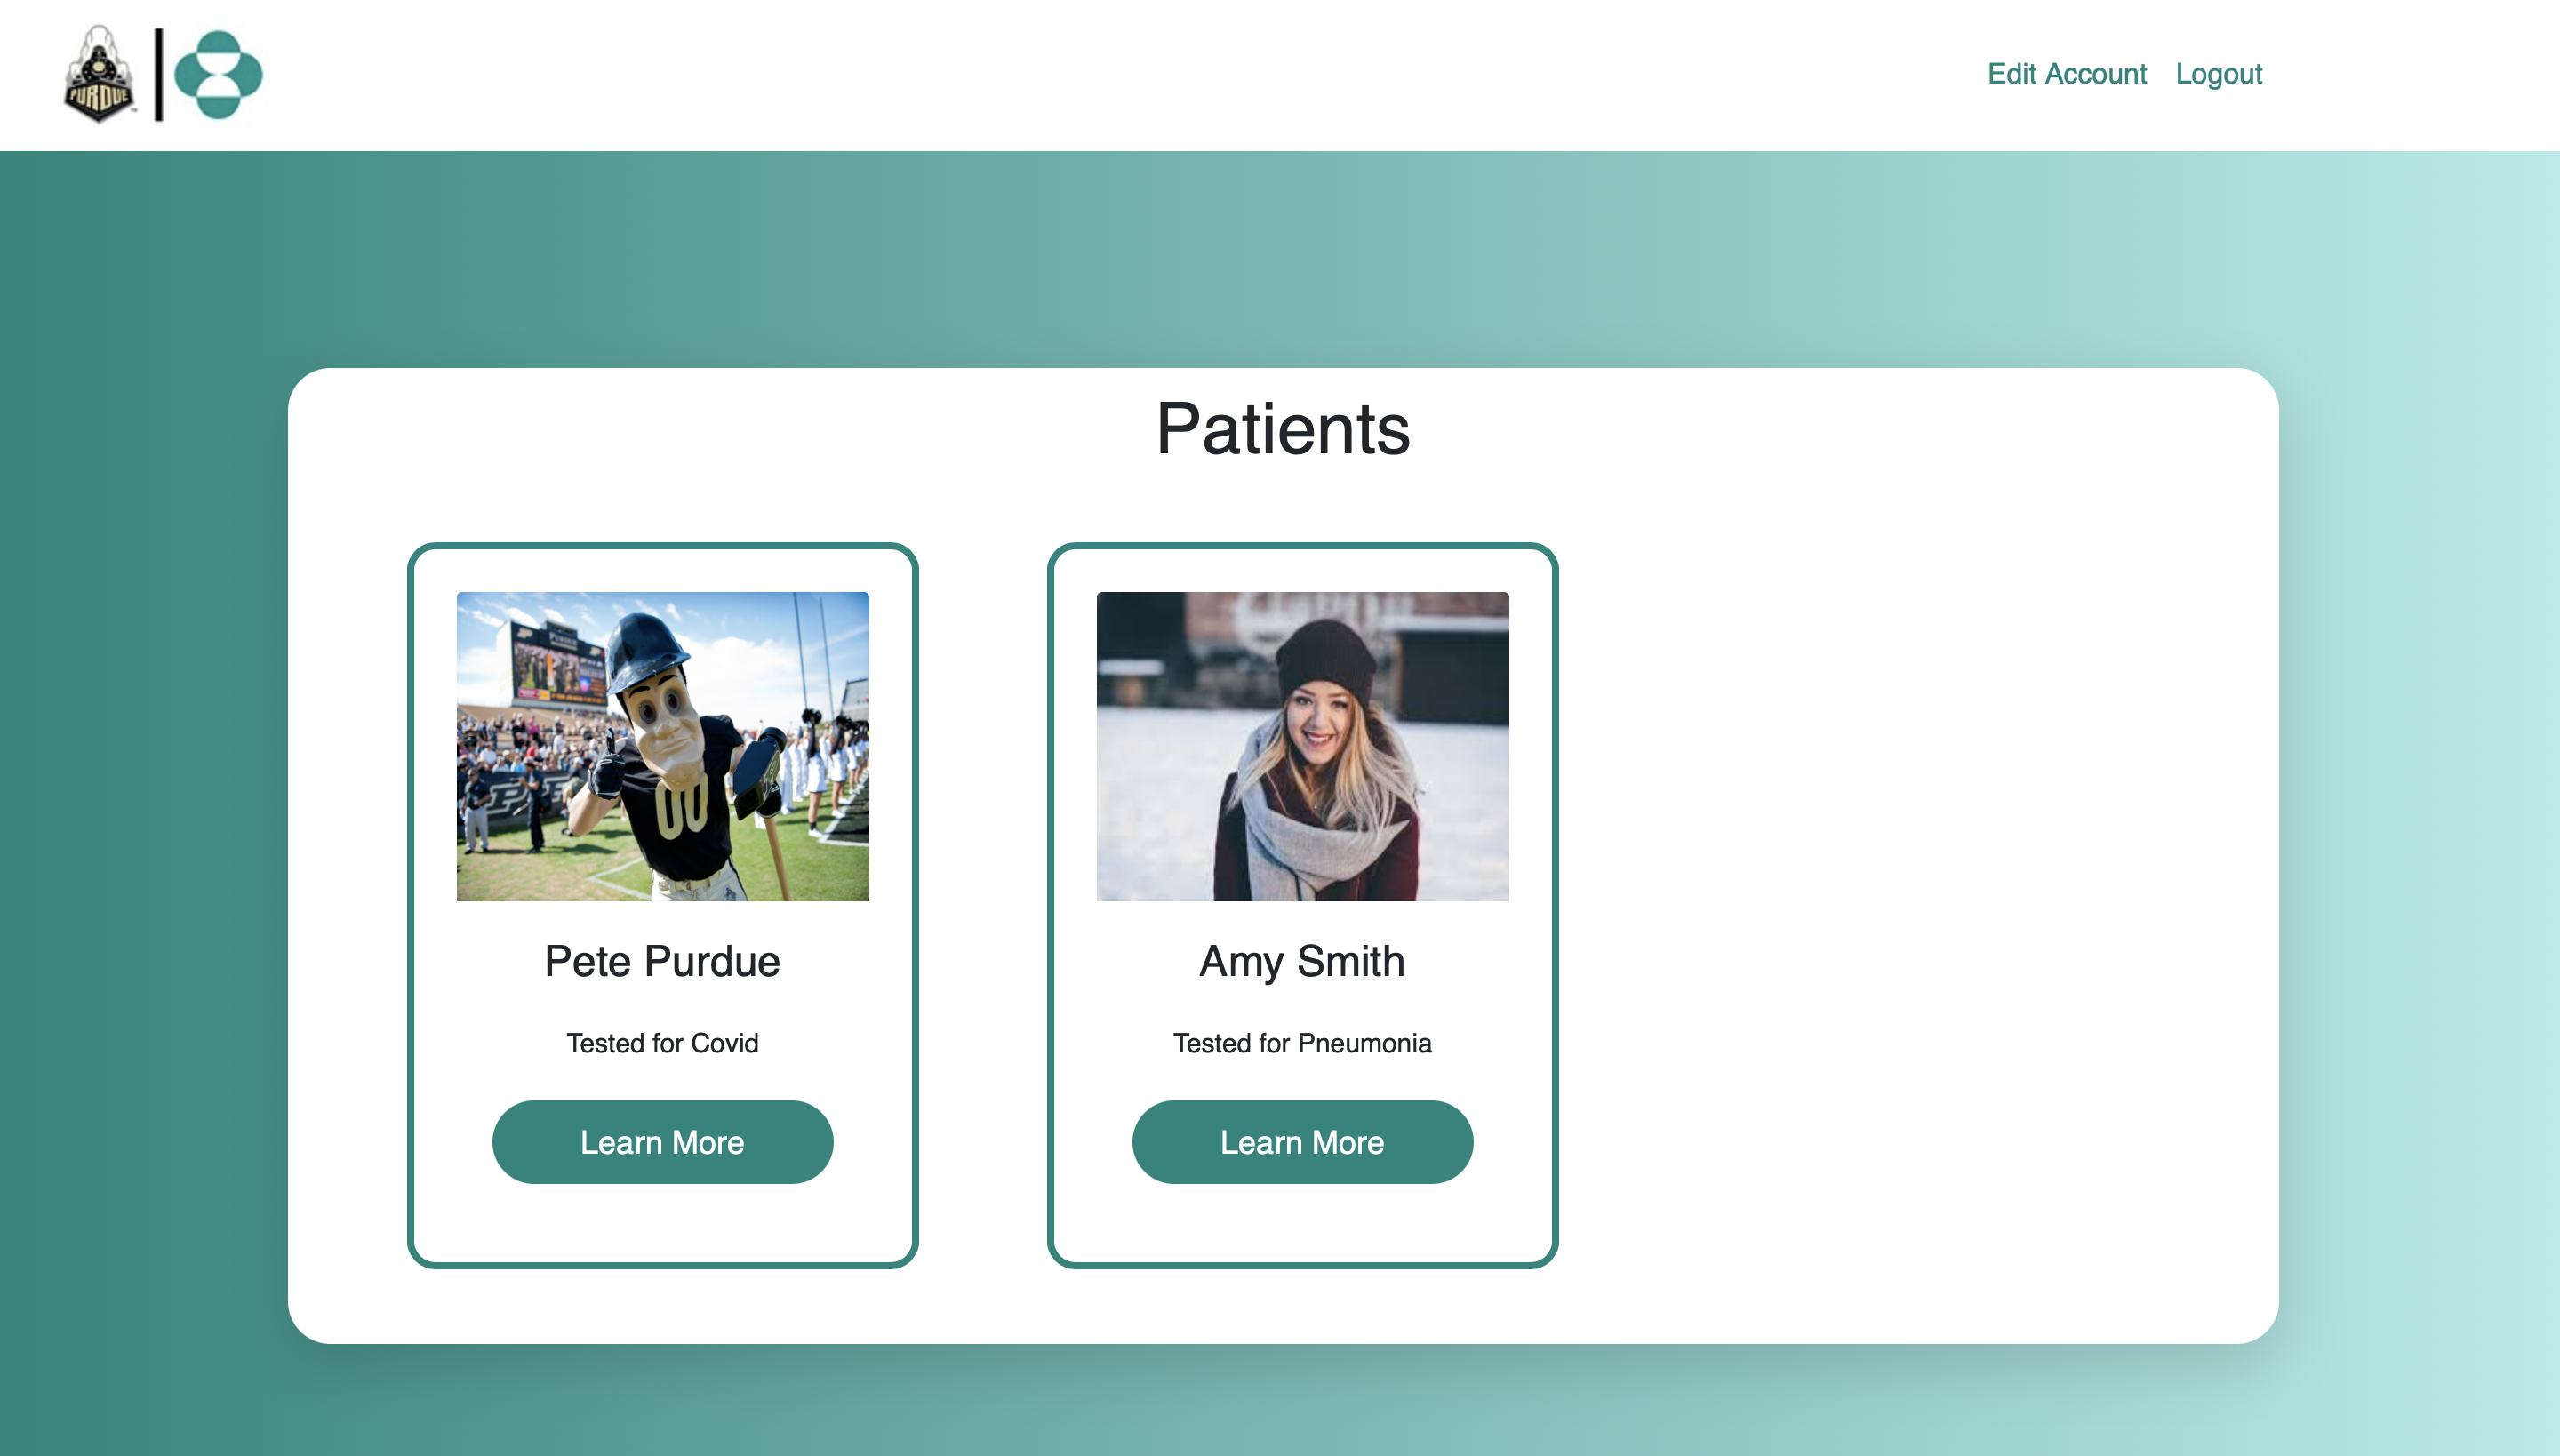
\includegraphics{images/Patients_gallery_page.png}
\caption{}
\end{figure}

\paragraph{Patient Information}\label{patient-information}

Patient information pages exist for each patient and contain basic
information about the patient and links to survey data, study notes, and
Fitbit data, along with links to visualizations, videos, and patient
analysis.

\begin{figure}
\centering
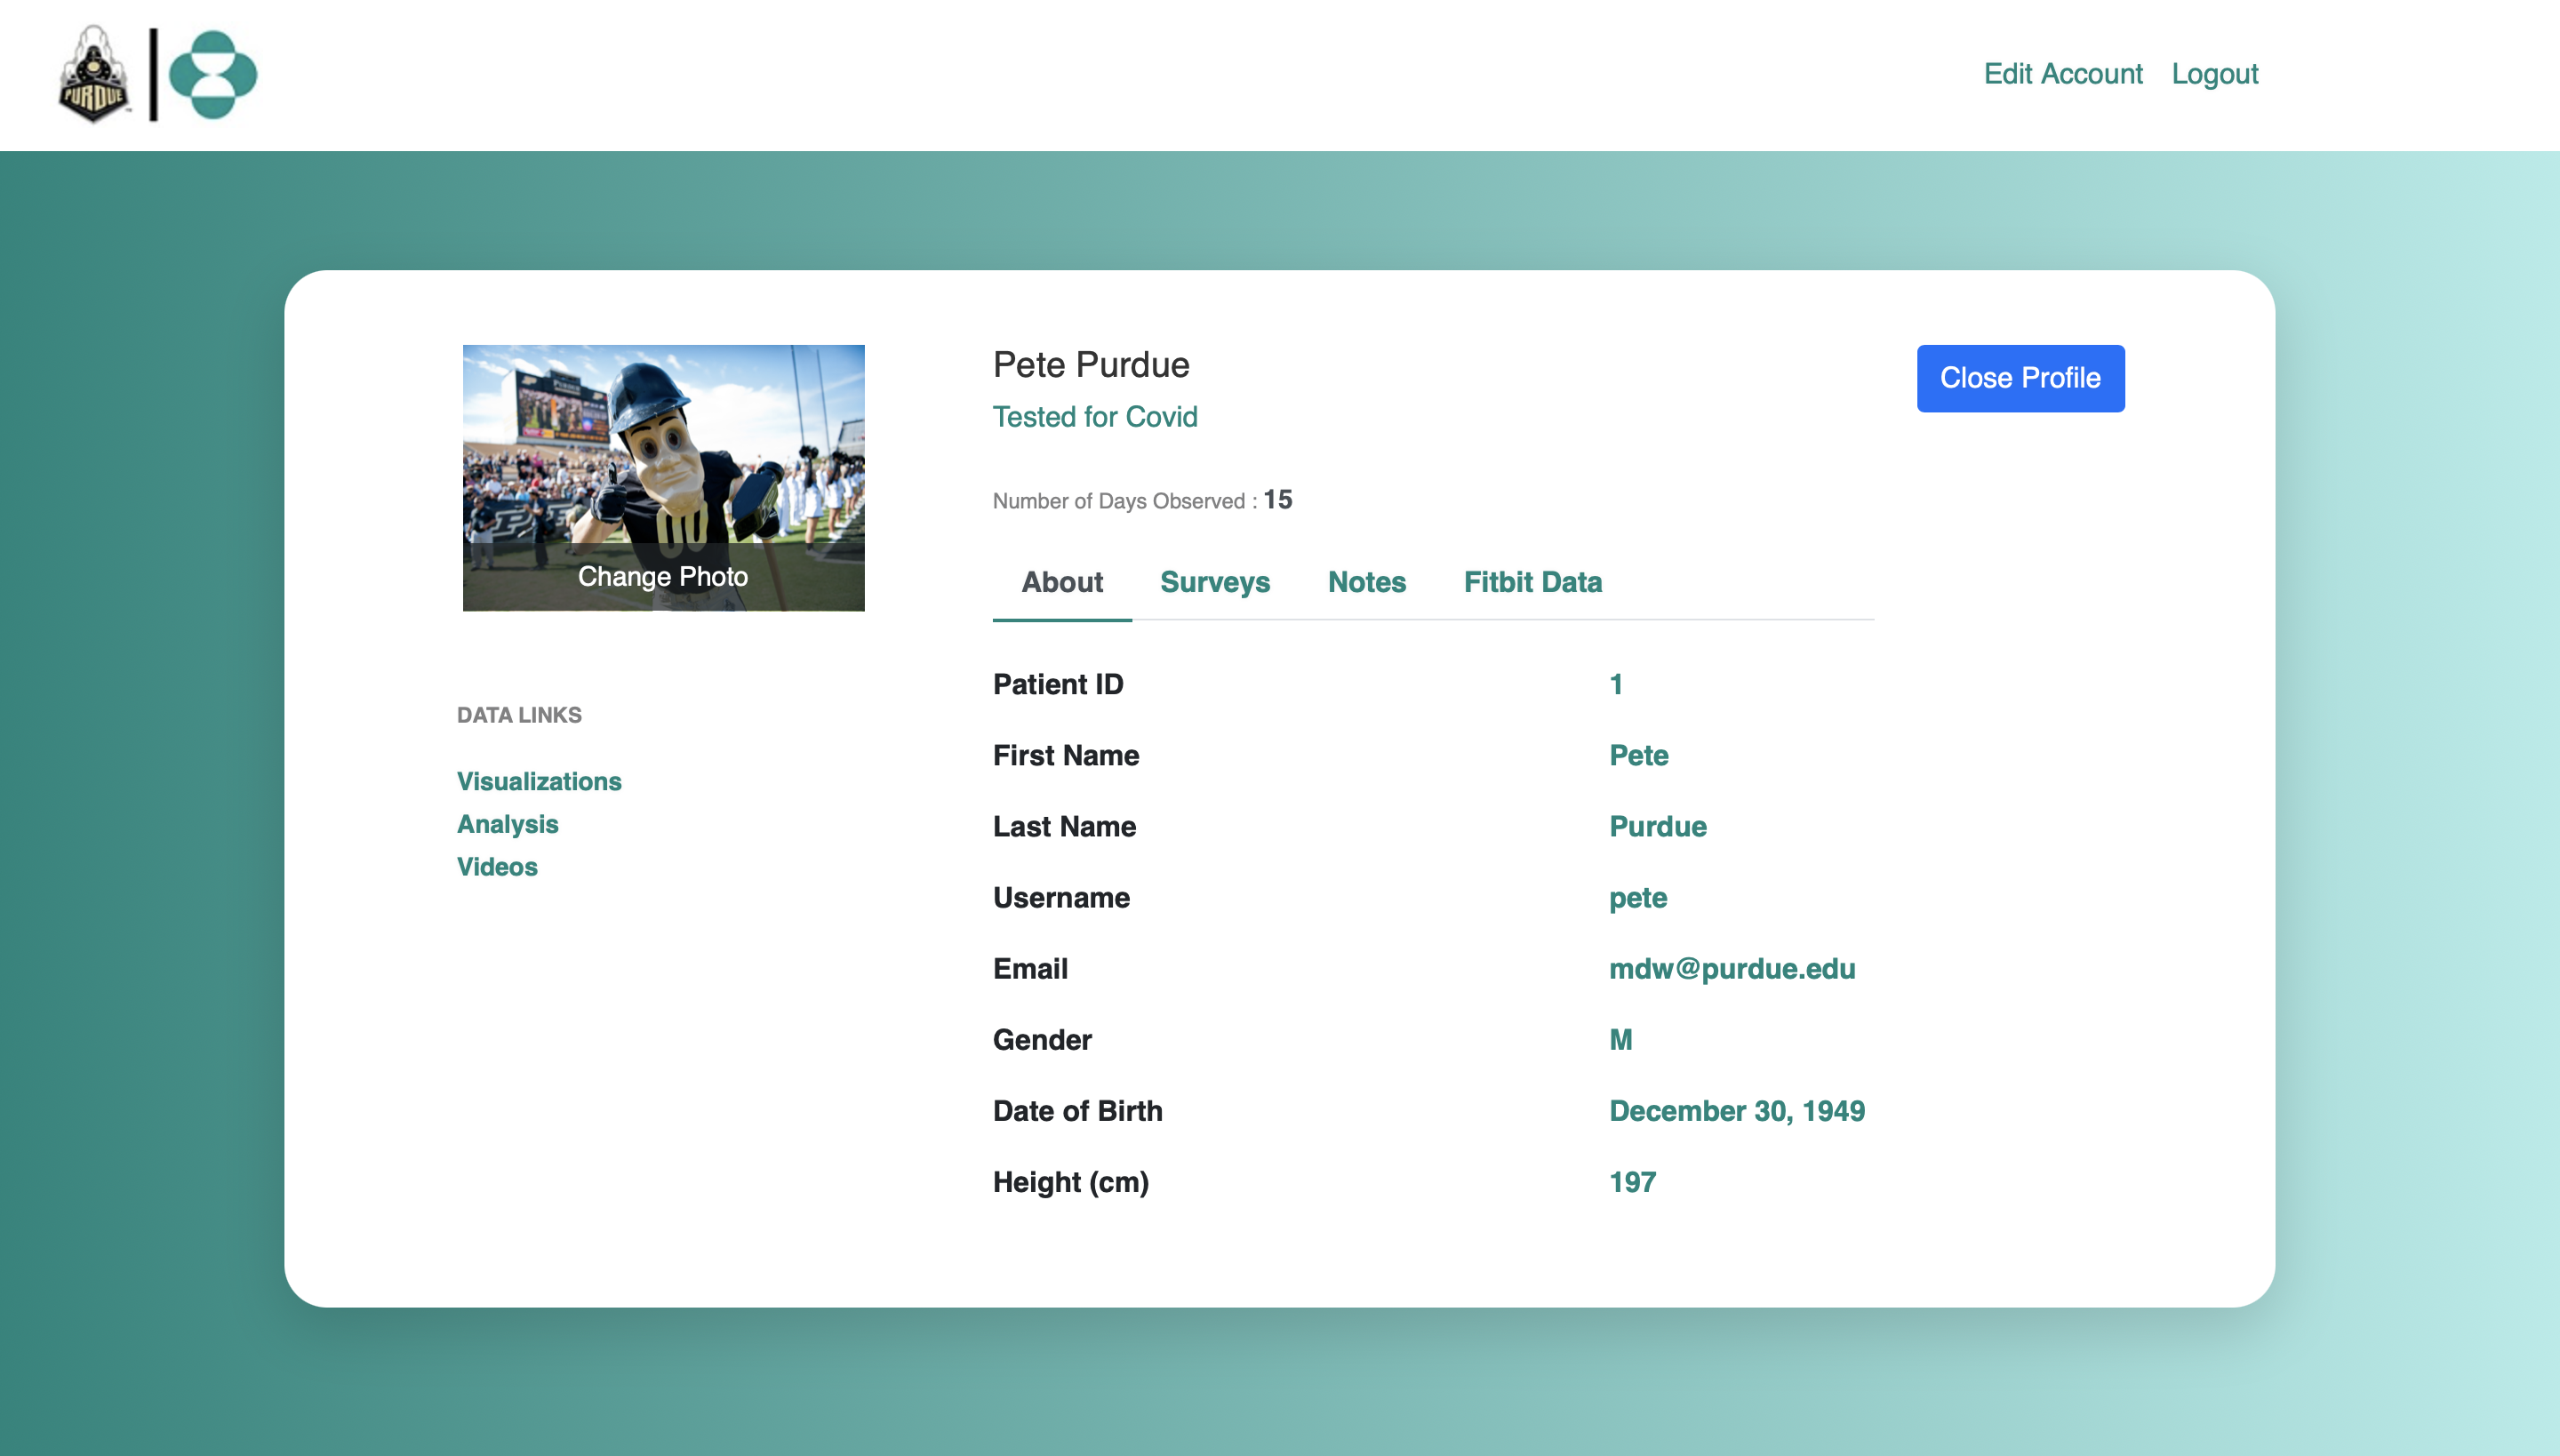
\includegraphics{images/Information_page.png}
\caption{}
\end{figure}

\paragraph{Phone Survey Data}\label{phone-survey-data}

The phone survey tab shows a list of all patient survey entries from the
phone application, and when clicked on, shows the details and results of
the survey.

\href{images/phone_survey_gif.gif}{link}

\paragraph{Scientist Notes}\label{scientist-notes}

The scientist notes tab shows a list of all scientist-reported surveys
containing information about the patient. New entries can be added and
old surveys can be updated.

\href{images/scientist_note_gif.gif}{link}

\paragraph{Fitbit Data}\label{fitbit-data}

The Fitbit Data tab contains a table of the most important information
collected by the Fitbit. This is updated daily. More data visualization
and analysis can be found on other pages (future work).

\begin{figure}
\centering
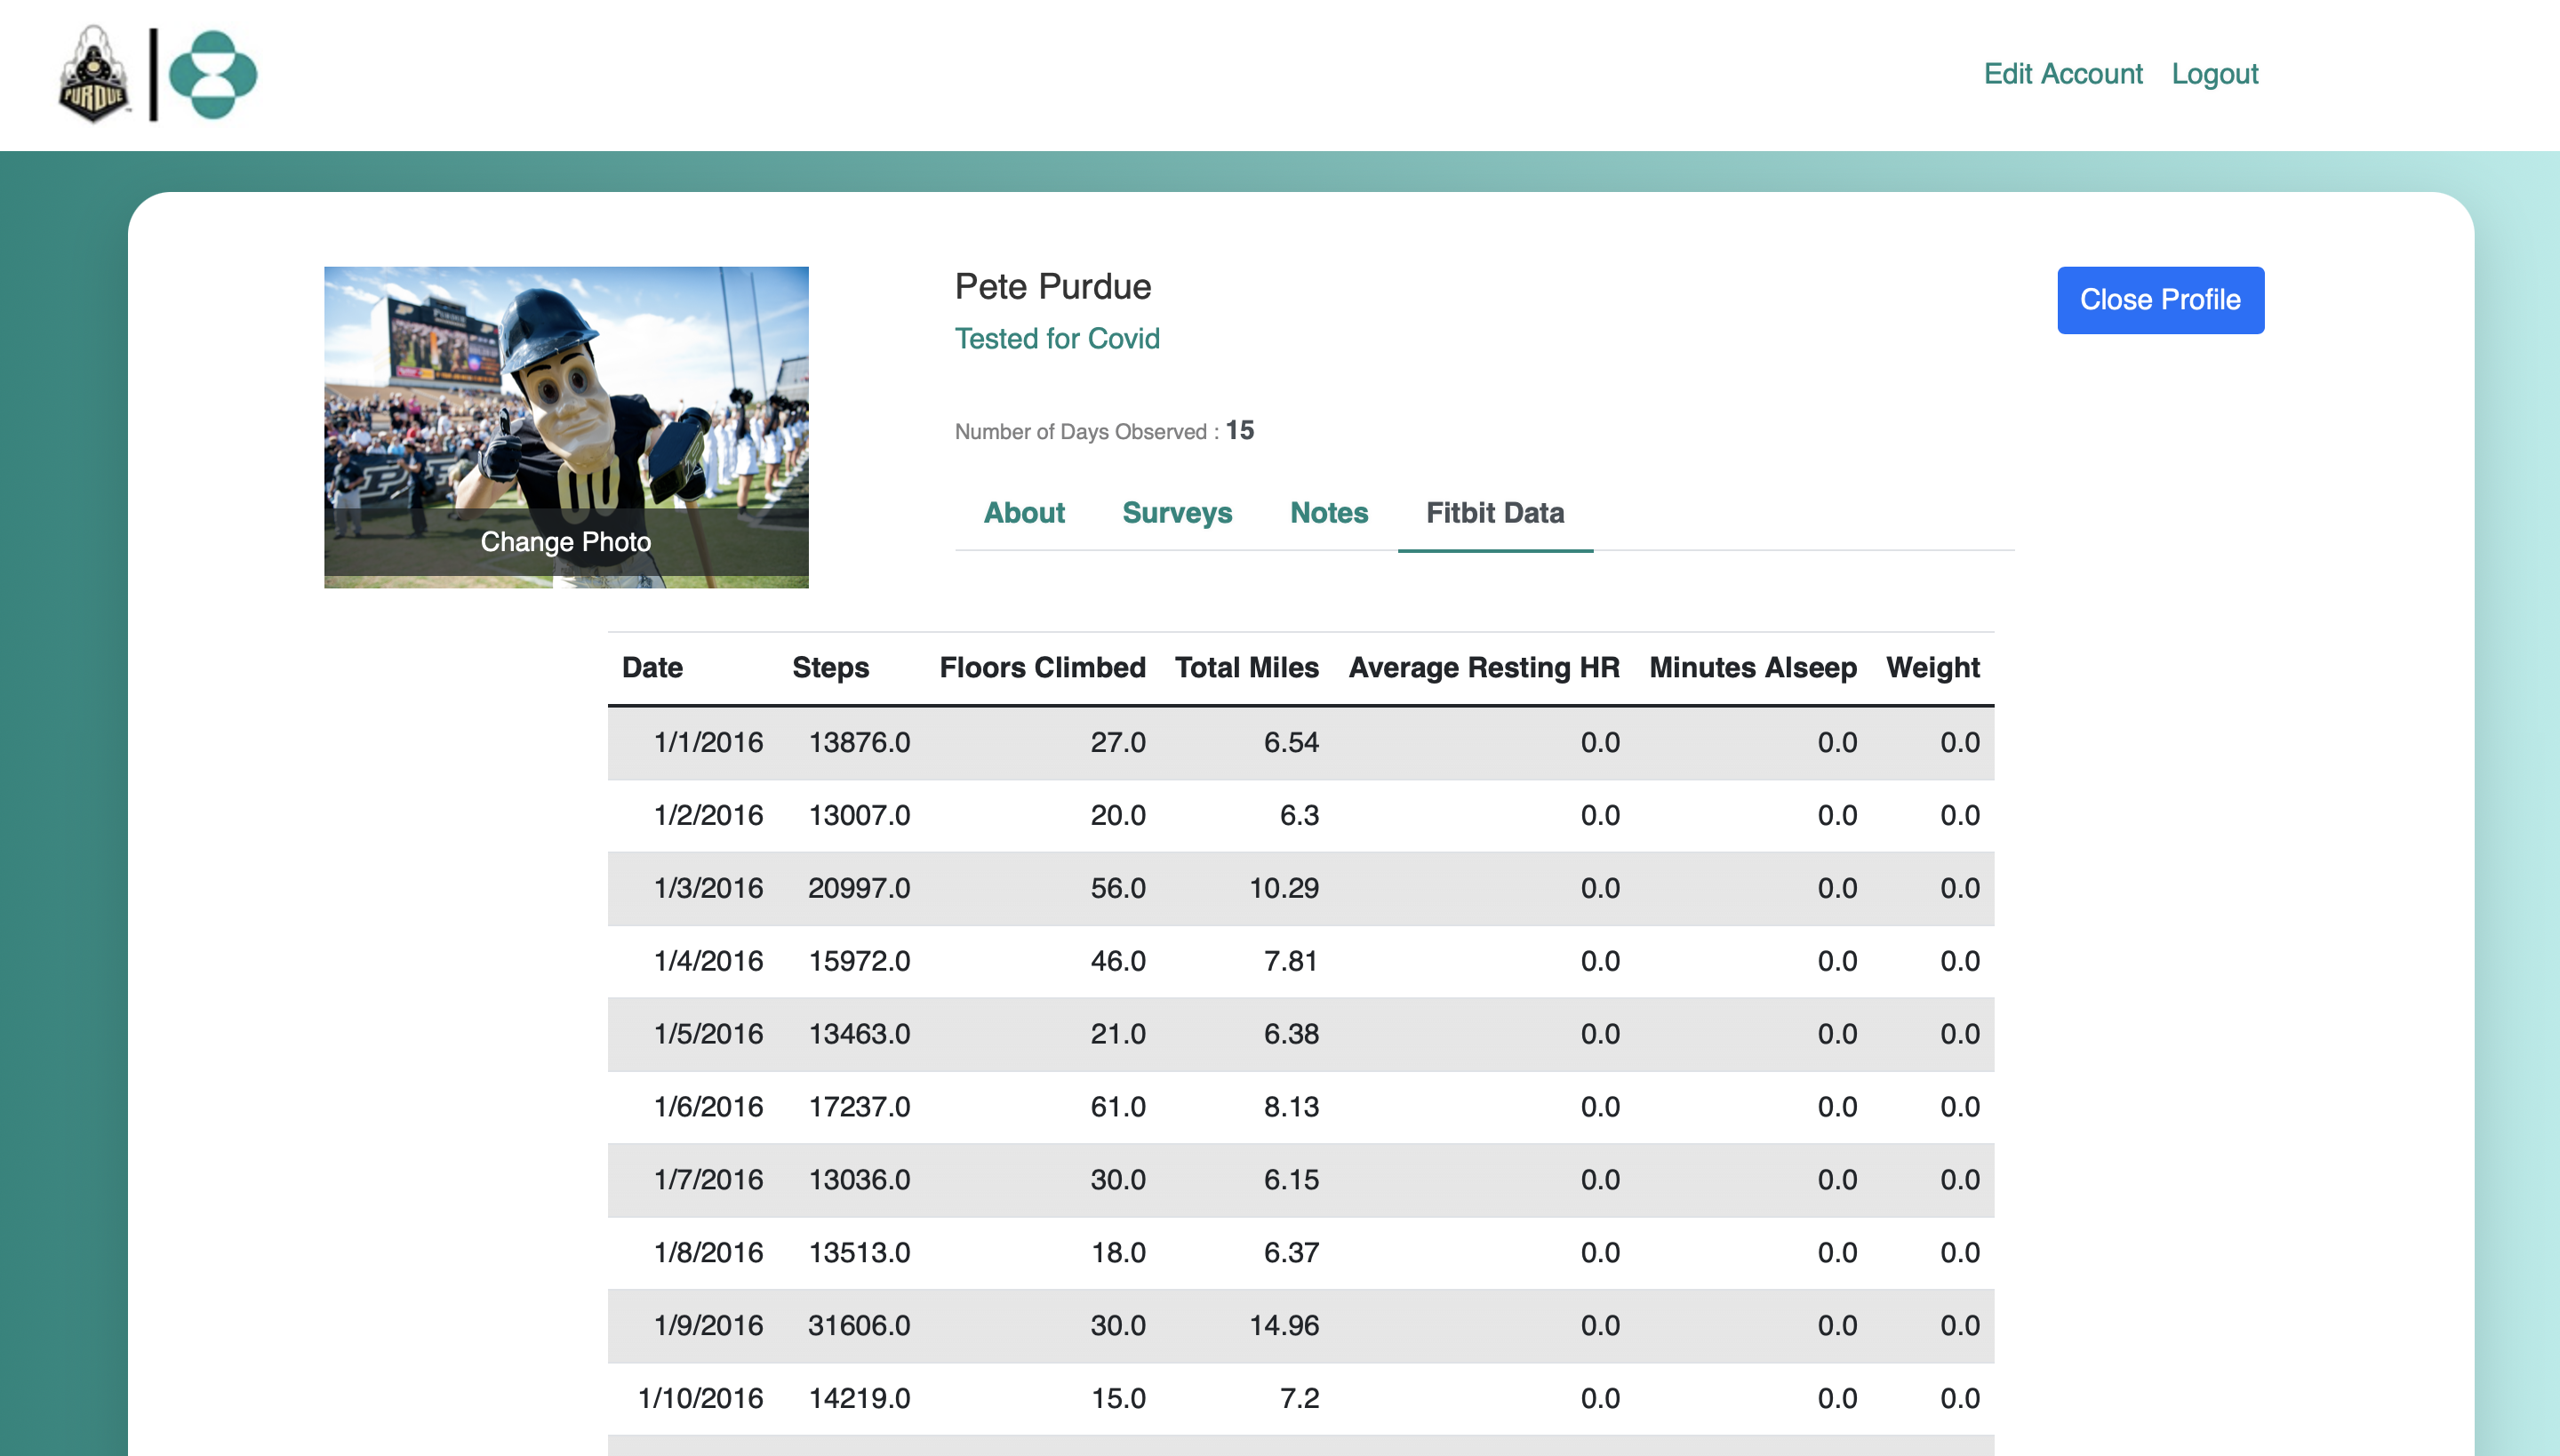
\includegraphics{images/Fitbit_page.png}
\caption{}
\end{figure}

\subsubsection{HTML Scripts}\label{html-scripts}

All HTML files must be stored in a folder called ``templates'' that is
in the same directory as the routes. Typical file structure is shown
below:

\begin{figure}
\centering
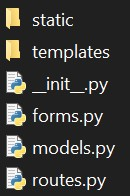
\includegraphics{images/file_structure.jpg}
\caption{}
\end{figure}

where ``static'' contains all CSS files and images and ``templates''
contains all HTML files.

To learn the HTML and CSS required for this project, we watched
tutorials on each.

\url{https://www.youtube.com/watch?v=UB1O30fR-EE} (1 hr)

\url{https://www.youtube.com/watch?v=yfoY53QXEnI} (1 hr 25 min)

The basics of these languages are simple. HTML is mostly knowing the
different ``tags'' and understanding how linking those tags to classes
and CSS. These two tutorials cover that much better than I can. Most of
the team had little to no experience with HTML/CSS, which explains why
our HTML and CSS files are all over the place. We incorporated Bootstrap
as it made forms easier to create and improved their appearance, as well
as allowed for a navigation bar.

\section{Documentation for the packages we
used:}\label{documentation-for-the-packages-we-used}

Flask: \url{https://flask.palletsprojects.com/en/1.1.x/}

SQLAlchemy: \url{https://flask-sqlalchemy.palletsprojects.com/en/2.x/}

Bcrypt: \url{https://flask-bcrypt.readthedocs.io/en/latest/}

Flask Login: \url{https://flask-login.readthedocs.io/en/latest/}

Flask Forms:
\url{https://flask.palletsprojects.com/en/1.1.x/patterns/wtforms/}

Bootstrap: \url{https://getbootstrap.com/}

\end{document}
